\documentclass[a4paper]{article}
\usepackage{graphicx}

\usepackage[  margin=2.5cm,  includefoot,  footskip=30pt,]{geometry}

%\usepackage[cm]{fullpage}
\usepackage{bm}
\usepackage{listings}
%\usepackage{color}
\usepackage{amsmath}
\usepackage{amsfonts}
\usepackage{hyperref}
%\usepackage{xcolor}
\usepackage{mdframed}
\usepackage{makeidx} 
\usepackage{xargs}
\usepackage[pdftex,dvipsnames]{xcolor}
\usepackage[colorinlistoftodos,prependcaption,textsize=tiny]{todonotes}
\hypersetup{
    colorlinks,
    citecolor=black,
    filecolor=black,
    linkcolor=black,
    urlcolor=black
}
\lstset{ 
  language=Python,
  backgroundcolor=\color{white},   % choose the background color; you must add \usepackage{color} or \usepackage{xcolor}; should come as last argument
  basicstyle=\footnotesize,        % the size of the fonts that are used for the code
  breakatwhitespace=false,         % sets if automatic breaks should only happen at whitespace
  breaklines=true,                 % sets automatic line breaking
  captionpos=b,                    % sets the caption-position to bottom
  frame=single,                    % adds a frame around the code
  keepspaces=true,                 % keeps spaces in text, useful for keeping indentation of code (possibly needs columns=flexible)
  keywordstyle=\color{blue},       % keyword style
}

\newcommand{\nn}{\nonumber}
\newcommand{\A}{{\mathbb{A}}}
\newcommand{\K}{{\mathbb{K}}}
\newcommand{\G}{{\mathbb{G}}}
\newcommand{\Z}{{\mathbb{Z}}}
\newcommand{\W}{{\mathbb{W}}}
\newcommand{\LLL}{{\mathbb{L}}}
\newcommand{\SSS}{{\mathbb{S}}}
\newcommand{\fieldstone}{{\bf fieldstone}}

\newcommandx{\unsure}[2][1=]{\todo[linecolor=red,backgroundcolor=red!25,bordercolor=red,#1]{#2}}
\newcommandx{\change}[2][1=]{\todo[linecolor=blue,backgroundcolor=blue!25,bordercolor=blue,#1]{#2}}
\newcommandx{\info}[2][1=]{\todo[linecolor=OliveGreen,backgroundcolor=OliveGreen!25,bordercolor=OliveGreen,#1]{#2}}
\newcommandx{\improvement}[2][1=]{\todo[linecolor=Plum,backgroundcolor=Plum!15,bordercolor=Plum,#1]{#2}}
\newcommandx{\thiswillnotshow}[2][1=]{\todo[disable,#1]{#2}}

%%%%%%%%%%%%%%%%%%%%%%%%%%%%%%%%%%%%%%%%%%%%%%%%%%%%%%%%%%%%%%%%%%%%%%%%%%%%%%%%%%%%%%%%%%%%%%%%%%%
%%%%%%%%%%%%%%%%%%%%%%%%%%%%%%%%%%%%%%%%%%%%%%%%%%%%%%%%%%%%%%%%%%%%%%%%%%%%%%%%%%%%%%%%%%%%%%%%%%%
%%%%%%%%%%%%%%%%%%%%%%%%%%%%%%%%%%%%%%%%%%%%%%%%%%%%%%%%%%%%%%%%%%%%%%%%%%%%%%%%%%%%%%%%%%%%%%%%%%%
%%%%%%%%%%%%%%%%%%%%%%%%%%%%%%%%%%%%%%%%%%%%%%%%%%%%%%%%%%%%%%%%%%%%%%%%%%%%%%%%%%%%%%%%%%%%%%%%%%%
%%%%%%%%%%%%%%%%%%%%%%%%%%%%%%%%%%%%%%%%%%%%%%%%%%%%%%%%%%%%%%%%%%%%%%%%%%%%%%%%%%%%%%%%%%%%%%%%%%%

\title{The Finite Element Method in Geodynamics}

\author{C. Thieulot}

\makeindex 
\begin{document}

\maketitle

\tableofcontents

\newpage
%%%%%%%%%%%%%%%%%%%%%%
\section{Introduction}

{\color{red} \huge WARNING: this is work in progress}

practical hands-on approach

as little as possible jargon

no mathematical proof

no optimised codes (readability over efficiency). avoiding as much as possible to have to look elsewhere.
very sequential, so unavoidable repetitions (jacobian, shape functions)

FE is one of several methods.

All the python scripts and this document are freely available at {\tt https://github.com/cedrict/fieldstone}.

\subsection{Acknowledgments}

Jean Braun, Philippe Fullsack, Arie van den Berg.
Lukas van de Wiel. Robert Myhill.
Menno, Anne
Too many BSc and MSc students to name indivisually, although Job Mos did produce the
very first version of fieldstone as part of his MSc thesis.
The ASPECT team in general and Wolfgang Bangerth and Timo Heister in particular.

%--------------------------------
\subsection{Essential literature}

\begin{center}
a)
\includegraphics[height=3.74cm]{images/literature/gerya_book}
b)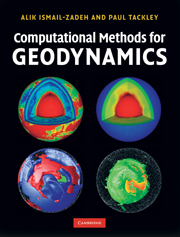
\includegraphics[height=3.74cm]{images/literature/tackley_book}
c)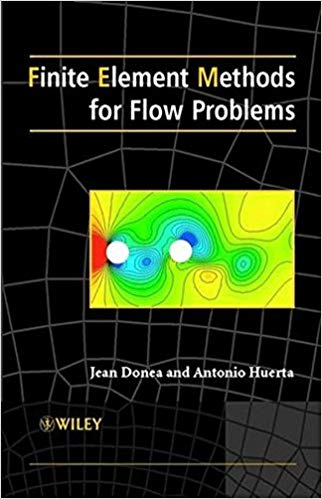
\includegraphics[height=3.74cm]{images/literature/donea_huerta_book}
d)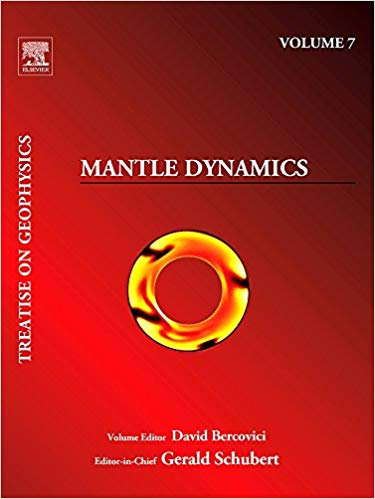
\includegraphics[height=3.74cm]{images/literature/bercovici_book}
e)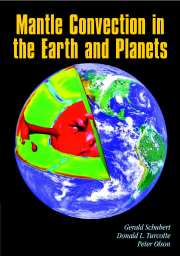
\includegraphics[height=3.74cm]{images/literature/sto_book}\\
%a) \url{https://doi.org/10.1017/CBO9780511809101}
%b) \url{https://doi.org/10.1017/CBO9780511780820}
%c) \url{https://www.wiley.com/en-us/Finite+Element+Methods+for+Flow+Problems-p-9780471496663}
%d) \url{https://www.elsevier.com/books/treatise-on-geophysics-volume-7/bercovici/978-0-444-51935-1}
\end{center}

%---------------------------------------
\subsection{Installation}

\begin{verbatim}
python3.6 -m pip install --user numpy scipy matplotlib
\end{verbatim}

\newpage
%%%%%%%%%%%%%%%%%%%%%%
\section{The physical equations of Fluid Dynamics}

\begin{center}
\begin{tabular}{lll}
\hline
Symbol & meaning & unit \\
\hline
\hline
$t$ & Time & s \\
$x,y,z$ & Cartesian coordinates & m \\
${\bm v}$ & velocity vector & m$\cdot$ s$^{-1}$\\
$\rho$ & mass density & kg/m$^3$ \\
$\eta$ & dynamic viscosity &  Pa$\cdot$ s \\
$\lambda$ & penalty parameter & Pa$\cdot$ s \\
$T$ & temperature & K \\
${\bm \nabla}$ & gradient operator & m$^{-1}$ \\
${\bm \nabla}\cdot$ & divergence operator & m$^{-1}$ \\
$p$ & pressure & Pa\\
$\dot{\bm \varepsilon}({\bm v})$ & strain rate tensor & s$^{-1}$ \\
$\alpha$ & thermal expansion coefficient & K$^{-1}$ \\
$k$ & thermal conductivity & W/(m $\cdot$ K) \\
$C_p$ & Heat capacity & J/K \\
$H$ & intrinsic specific heat production & W/kg\\
$\beta_T$ & isothermal compressibility & Pa$^{-1}$  \\
${\bm \tau}$ & deviatoric stress tensor & Pa \\
${\bm \sigma}$ & full stress tensor & Pa \\
\hline
\end{tabular}
\end{center}

%------------------------------------------------------------------------
\subsection{The heat transport equation - energy conservation equation}

Let us start from the heat transport equation as shown in Schubert, Turcotte and Olson \cite{scto01}:
\[
\rho C_p \frac{DT}{Dt} - \alpha T \frac{Dp}{Dt} = {\bm \nabla} \cdot k {\bm \nabla} T + \Phi + \rho H  
\]
with $D/Dt$ being the total derivatives so that 
\[
\frac{DT}{Dt} = \frac{\partial T}{\partial t} + {\bm v}\cdot {\bm \nabla}T
\quad\quad
\frac{Dp}{Dt} = \frac{\partial p}{\partial t} + {\bm v}\cdot {\bm \nabla}p
\]
Solving for temperature, this equation is often rewritten as follows:
\begin{mdframed}[backgroundcolor=blue!5]
\[
\rho C_p \frac{DT}{Dt} - {\bm \nabla} \cdot k {\bm \nabla} T =  \alpha T \frac{Dp}{Dt} + \Phi + \rho H  
\]
\end{mdframed}

A note on the shear heating term $\Phi$: In many publications, $\Phi$ 
is given by $\Phi=\tau_{ij}\partial_j u_i={\bm \tau}:{\bm \nabla}{\bm v}$.

\begin{eqnarray}
\Phi 
&=& \tau_{ij}\partial_j u_i \nonumber\\
&=& 2 \eta \dot{\varepsilon}_{ij}^d\partial_j u_i \nonumber\\
&=& 2 \eta \frac{1}{2}\left( \dot{\varepsilon}_{ij}^d\partial_j u_i + \dot{\varepsilon}_{ji}^d\partial_i u_j \right) \nonumber\\
&=& 2 \eta \frac{1}{2}\left( \dot{\varepsilon}_{ij}^d\partial_j u_i + \dot{\varepsilon}_{ij}^d\partial_i u_j \right) \nonumber\\
&=& 2 \eta  \dot{\varepsilon}_{ij}^d  \frac{1}{2}\left(\partial_j u_i + \partial_i u_j \right) \nonumber\\
&=& 2 \eta  \dot{\varepsilon}_{ij}^d   \dot{\varepsilon}_{ij} \nonumber\\
&=& 2 \eta  \dot{\bm \varepsilon}^d :  \dot{\bm \varepsilon} \nonumber\\
&=& 2 \eta  \dot{\bm \varepsilon}^d : \left( \dot{\bm \varepsilon}^d +\frac{1}{3} ({\bm \nabla}\cdot{\bm v}) {\bm 1} \right)\nonumber\\
&=& 2 \eta  \dot{\bm \varepsilon}^d : \dot{\bm \varepsilon}^d 
+ 2 \eta  \dot{\bm \varepsilon}^d : {\bm 1} ({\bm \nabla}\cdot{\bm v}) \nonumber\\ 
&=& 2 \eta  \dot{\bm \varepsilon}^d : \dot{\bm \varepsilon}^d 
\end{eqnarray}
Finally
\[
\Phi = {\bm \tau}:{\bm \nabla}{\bm v} = 2 \eta  \dot{\bm \varepsilon}^d : \dot{\bm \varepsilon}^d
= 2 \eta \left( (\dot{\varepsilon}_{xx}^d)^2 + (\dot{\varepsilon}_{yy}^d)^2 + 2(\dot{\varepsilon}_{xy}^d)^2 \right)
\]

%------------------------------------------------------------------------
\subsection{The momentum conservation equations} 

Because the Prandlt number is virtually zero in Earth science applications the Navier Stokes 
equations reduce to the Stokes equation:
\[
{\bm \nabla}\cdot {\bm \sigma} + \rho {\bm g} = 0
\]
Since 
\[
{\bm \sigma} = -p {\bm 1} + {\bm \tau}
\]
it also writes
\[
-{\bm \nabla}p + {\bm \nabla}\cdot {\bm \tau} + \rho {\bm g} = 0
\]
Using the relationship ${\bm \tau} = 2 \eta \dot{\bm \varepsilon}^d$ we arrive at 
\begin{mdframed}[backgroundcolor=blue!5]
\[
-{\bm \nabla}p + {\bm \nabla}\cdot (2 \eta \dot{\bm \varepsilon}^d ) + \rho {\bm g} = 0
\]
\end{mdframed}

%------------------------------------------------------------------------
\subsection{The mass conservation equations} 

The mass conservation equation is given by
\[
\frac{D\rho}{Dt} + \rho {\bm \nabla}\cdot{\bm v} = 0
\]
or, 
\begin{mdframed}[backgroundcolor=blue!5]
\[
\frac{\partial \rho}{\partial t} + {\bm \nabla}\cdot(\rho {\bm v}) = 0
\]
\end{mdframed}
In the case of an incompressible flow, then $\partial \rho/\partial t=0$ and 
${\bm \nabla}\rho=0$, i.e. $D\rho/Dt=0$ and the remaining equation is simply:
\[
{\bm \nabla}\cdot{\bm v} = 0
\]

\subsection{The equations in ASPECT manual}
The following is lifted off the ASPECT manual.
We focus on the system of equations in a $d=2$- or $d=3$-dimensional
domain $\Omega$ that describes the motion of a highly viscous fluid driven
by differences in the gravitational force due to a density that depends on
the temperature. In the following, we largely follow the exposition of this
material in Schubert, Turcotte and Olson \cite{scto01}.

Specifically, we consider the following set of equations for velocity $\mathbf
u$, pressure $p$ and temperature $T$:
\begin{align}
  \label{eq:stokes-1}
  -\nabla \cdot \left[2\eta \left(\dot\varepsilon(\bm v)
                                  - \frac{1}{3}(\nabla \cdot \bm v)\mathbf 1\right)
                \right] + \nabla p &=
  \rho \bm g
  &
  & \textrm{in $\Omega$},
  \\
  \label{eq:stokes-2}
  \nabla \cdot (\rho \bm v) &= 0
  &
  & \textrm{in $\Omega$},
  \\
  \label{eq:temperature}
  \rho C_p \left(\frac{\partial T}{\partial t} + \bm v\cdot\nabla T\right)
  - \nabla\cdot k\nabla T
  &=
  \rho H
  \notag
  \\
  &\quad
  +
  2\eta
  \left(\dot\varepsilon(\bm v) - \frac{1}{3}(\nabla \cdot \bm v)\mathbf 1\right)
  :
  \left(\dot\varepsilon(\bm v) - \frac{1}{3}(\nabla \cdot \bm v)\mathbf 1\right)
  \\
  &\quad
  +\alpha T \left( \bm v \cdot \nabla p \right)
  \notag
  \\
  &\quad
  &
  & \textrm{in $\Omega$},
  \notag
\end{align}
where $\dot{\bm \varepsilon}(\mathbf u) = \frac{1}{2}(\nabla \mathbf u + \nabla\mathbf
u^T)$ is the symmetric gradient of the velocity (often called the
\textit{strain rate}).%

In this set of equations, \eqref{eq:stokes-1} and \eqref{eq:stokes-2}
represent the compressible Stokes equations in which $\mathbf v=\mathbf
v(\mathbf x,t)$ is the velocity field and $p=p(\mathbf x,t)$ the pressure
field. Both fields depend on space $\mathbf x$ and time $t$. Fluid flow is
driven by the gravity force that acts on the fluid and that is proportional to
both the density of the fluid and the strength of the gravitational pull.

Coupled to this Stokes system is equation \eqref{eq:temperature} for the
temperature field $T=T(\mathbf x,t)$ that contains heat conduction terms as
well as advection with the flow velocity $\mathbf v$. The right hand side
terms of this equation correspond to
\begin{itemize}
\item internal heat production for example due to radioactive decay;
\item friction (shear) heating;
\item adiabatic compression of material;
\end{itemize}

In order to arrive at the set of equations that ASPECT solves, 
we need to 
\begin{itemize}
\item neglect the $\partial p/\partial t$. {\color{red}WHY?}
\item neglect the $\partial \rho / \partial t$ . {\color{red}WHY?}
\end{itemize}
from equations above. 

----------------------------------------

Also, their definition of the shear heating term $\Phi$ is:
\[
\Phi = k_B ({\bm \nabla}\cdot{\bm v})^2 + 2\eta \dot{\bm \varepsilon}^d:\dot{\bm \varepsilon}^d
\]
For many fluids the bulk viscosity $k_B$ is very small and is often taken to be zero, an assumption known
as the Stokes assumption: $k_B=\lambda+2\eta/3=0$. \index{bulk viscosity}
Note that $\eta$ is the dynamic viscosity and $\lambda$ the second viscosity. \index{dynamic viscosity}
\index{second viscosity}
Also, 
\[
{\bm \tau}=2\eta \dot{\bm \varepsilon} + \lambda ({\bm \nabla}\cdot{\bm v}) {\bm 1}
\]
but since $k_B=\lambda+2\eta/3=0$, then $\lambda=-2\eta/3$ so 
\[
{\bm \tau}=2\eta \dot{\bm \varepsilon} -\frac{2}{3}\eta ({\bm \nabla}\cdot{\bm v}) {\bm 1} = 2\eta \dot{\bm \varepsilon}^d
\]







\newpage
%---------------------------------
\subsection{the Boussinesq approximation: an Incompressible flow}

\index{Boussinesq}

[from aspect manual]
The Boussinesq approximation assumes that the density can be
considered constant in all occurrences in the equations with the exception of
the buoyancy term on the right hand side of \eqref{eq:stokes-1}. The primary
result of this assumption is that the continuity equation \eqref{eq:stokes-2}
will now read
\[
{\bm \nabla}\cdot{\bm v} = 0
\]
This implies that the strain rate tensor is deviatoric.
Under the Boussinesq approximation, the equations are much simplified:

\begin{align}
  \label{eq:stokes-1}
  -\nabla \cdot \left[2\eta \dot{\bm \varepsilon}(\bm v)
                \right] + \nabla p &=
  \rho \bm g
  &
  & \textrm{in $\Omega$},
  \\
  \label{eq:stokes-2}
  \nabla \cdot (\rho \bm v) &= 0
  &
  & \textrm{in $\Omega$},
  \\
  \label{eq:temperature}
  \rho_0 C_p \left(\frac{\partial T}{\partial t} + \bm v\cdot\nabla T\right)
  - \nabla\cdot k\nabla T
  &=
  \rho H
  &
  & \textrm{in $\Omega$}
\end{align}
Note that all terms on the rhs of the temperature equations have disappeared, with the exception 
of the source term.


\newpage
%%%%%%%%%%%%%%%%%%%%%%%%%%%%%%%%%%%%%%%%%%%%%%%%%%%%%%%%%%%%%%%%%%%%%%%%%%%%%%%%%%%%%%%%%%55
\subsection{Stokes equation for elastic medium}

What follows is mostly borrowed from Becker \& Kaus lecture notes.

%\begin{tabular}{|l|l|l|}
%\hline
%${\bm u}       $ & displacement vector &   \\
%${\bm \sigma}  $ & full stress tensor  & Pa\\
%${\bm \epsilon}$ & strain tensor       &   \\
%${\bm 1}       $ & unit tensor         &   \\
%${\bm f}       $ & body forces         &   \\
%\hline
%\end{tabular}

The strong form of the PDE that governs force balance in a medium is given by
\[
{\bm \nabla}\cdot{\bm \sigma}  + {\bm f} = {\bm 0}
\]
where ${\bm \sigma}$ is the stress tensor and ${\bm f}$ is a body force.

The stress tensor is related to the strain tensor through the generalised 
Hooke's law:
\begin{equation}
\sigma_{ij}=\sum_{kl}C_{ijkl}\epsilon{kl} \label{eq:one}
\end{equation}
where ${\bm C}$ is the fourth-order elastic tensor.
In the case of an isotropic material, this relationship simplifies to
\begin{equation}
\sigma_{ij}=\lambda \epsilon_{kk} \delta_{ij} + 2\mu \epsilon_{ij}
\quad\quad
or, 
\quad\quad
{\bm \sigma} = \lambda ({\bm \nabla}\cdot{\bm u})  {\bm 1} + 2\mu {\bm \epsilon}   \label{eq:two}
\end{equation}
where $\lambda$ is the Lam\'e parameter and $\mu$ is the shear modulus\footnote{It is also sometimes written $G$}.
The term ${\bm \nabla}\cdot{\bm u}$ is the isotropic dilation.

\index{Lam\'e parameter} \index{shear modulus}

The strain tensor is related to the displacement as follows: \index{strain tensor}
\[
{\bm \epsilon} = \frac{1}{2}({\bm \nabla}{\bm u} + {\bm \nabla}{\bm u}^T)
\]

The incompressibility (bulk modulus), $K$, is defined as $p=-K {\bm \nabla}\cdot{\bm u}$ 
where $p$ is the pressure with \index{bulk modulus}
\begin{eqnarray}
p&=&-\frac{1}{3}Tr({\bm \sigma}) \nonumber\\
 &=& -\frac{1}{3} [ \lambda ({\bm \nabla}\cdot{\bm u}) Tr[{\bm 1}] + 2 \mu Tr[{\bm \epsilon}]] \nonumber\\
 &=& -\frac{1}{3} [ \lambda ({\bm \nabla}\cdot{\bm u})  3  + 2 \mu  ({\bm \nabla}\cdot{\bm u}) ] \nonumber\\
 &=& -[ \lambda  + \frac{2}{3} \mu ]   ({\bm \nabla}\cdot{\bm u})  
\end{eqnarray}
so that $K=\lambda+\frac{2}{3}\mu$.

%or
%\[
%\mu=\frac{3K(1-2\nu)}{2(1+\nu)}
%\]


\paragraph{Remark}: Eq. (\ref{eq:one}) and (\ref{eq:two}) are analogous to the ones that one has to solve
in the context of viscous flow using the penalty method. In this case $\lambda$ is the penalty coefficient, 
${\bm u}$ is the velocity, and $\mu$ is then the dynamic viscosity.

%\begin{center}
%\includegraphics[width=15cm]{images/coeffs}\\
%{\small Homogeneous isotropic linear elastic materials have their elastic properties uniquely determined by any two moduli among these; thus, given any two, any other of the elastic moduli can be calculated according to these formulas.}
%\end{center}

The Lam\'e parameter and the shear modulus are also linked to $\nu$ the poisson ratio, 
and $E$, Young's modulus: \index{Poisson ratio} \index{Young's modulus}
\[
\lambda=\mu\frac{2\nu}{1-2\nu}
=\frac{\nu E}{(1+\nu)(1-2\nu)}
\quad\quad
{\rm with}
\quad\quad
E=2\mu(1+\nu)
\]
The shear modulus, expressed often in GPa, describes the material's response to shear stress.
The poisson ratio describes the response in the direction orthogonal to uniaxial stress.
The Young modulus, expressed in GPa, describes the material's strain response to uniaxial stress in the 
direction of this stress.


%%%%%%%%%%%%%%%%%%%%%%%%%%%%%%%%%%%%%%%%%%%%%%%%%%%%%%%%%%%%%%%%%%55
\newpage
\subsection{The strain rate tensor in all coordinate systems}

The strain rate tensor $\dot{\bm\varepsilon}$ is given by
\begin{equation}
\dot{\bm \varepsilon} = \frac{1}{2}( {\bm \nabla}{\bm v}+ {\bm \nabla}{\bm v}^T) 
\end{equation}

\subsubsection{Cartesian coordinates}
\begin{eqnarray}
\dot\varepsilon_{xx} &=& \frac{\partial u}{\partial x} \\
\dot\varepsilon_{yy} &=& \frac{\partial v}{\partial y} \\
\dot\varepsilon_{zz} &=& \frac{\partial w}{\partial z} \\
\dot\varepsilon_{yx} =
\dot\varepsilon_{xy} &=& \frac{1}{2} \left( \frac{\partial u}{\partial y} + \frac{\partial v}{\partial x}  \right)\\
\dot\varepsilon_{zx} =
\dot\varepsilon_{xz} &=& \frac{1}{2} \left( \frac{\partial u}{\partial z} + \frac{\partial w}{\partial x}  \right)\\
\dot\varepsilon_{zy} =
\dot\varepsilon_{yz} &=& \frac{1}{2} \left( \frac{\partial v}{\partial z} + \frac{\partial w}{\partial y}  \right)
\end{eqnarray}

\subsubsection{Polar coordinates}

\begin{eqnarray}
\dot\varepsilon_{rr} &=& \frac{\partial v_r}{\partial r} \\
\dot\varepsilon_{\theta\theta} &=& \frac{v_r}{r} + \frac{1}{r} \frac{\partial v_\theta}{\partial \theta}  \\
\dot\varepsilon_{\theta r} =
\dot\varepsilon_{r\theta} &=& \frac{1}{2} \left(   \frac{\partial v_\theta}{\partial r} - \frac{v_\theta}{r} 
+\frac{1}{r} \frac{\partial v_r}{\partial \theta}  \right) 
\end{eqnarray}

\subsubsection{Cylindrical coordinates}

http://eml.ou.edu/equation/FLUIDS/STRAIN/STRAIN.HTM

\subsubsection{Sperical coordinates}

\begin{eqnarray}
\dot\varepsilon_{rr} &=& \frac{\partial v_r}{\partial r} \\
\dot\varepsilon_{\theta\theta} &=& \frac{v_r}{r} + \frac{1}{r} \frac{\partial v_\theta}{\partial \theta}  \\
\dot\varepsilon_{\phi\phi} &=& \frac{1}{r \sin\theta} \frac{\partial v_\phi}{\partial \phi} \\
\dot\varepsilon_{\theta r} =
\dot\varepsilon_{r\theta}   &=& \frac{1}{2} \left( r \frac{\partial}{\partial r} (\frac{v_\theta}{r} ) 
+\frac{1}{r} \frac{\partial v_r}{\partial \theta} \right) \\
\dot\varepsilon_{\phi r} =
\dot\varepsilon_{r\phi}      &=&  \frac{1}{2} \left(  \frac{1}{r \sin\theta} \frac{\partial v_r}{\partial \phi} 
+ r \frac{\partial }{\partial r} (\frac{v_\phi}{r}) \right)  \\
\dot\varepsilon_{\phi \theta} =
\dot\varepsilon_{\theta\phi} &=& \frac{1}{2} \left( \frac{\sin \theta}{r} \frac{\partial }{\partial \theta} (\frac{v_\phi}{\sin\theta}) + \frac{1}{r \sin\theta} \frac{\partial v_\theta}{\partial \phi}    \right) 
\end{eqnarray}








\newpage
%------------------------------------------------------------------------------
\section{The building blocks of the Finite Element Method}

\subsection{Numerical integration}
As we will see later, using the Finite Element method to solve problems involves computing integrals which are more often than not too complex to be computed analytically/exactly. We will then need to compute them numerically.

[wiki] In essence, 
the basic problem in numerical integration is to compute an approximate solution to a definite integral
\[
\int_a^b f(x) dx
\]
to a given degree of accuracy.
This problem has been widely studied and we know that 
if $f(x)$ is a smooth function, and the domain of integration is bounded, there are many methods for approximating the integral to the desired precision.

There are several reasons for carrying out numerical integration.
\begin{itemize}
\item The integrand $f(x)$ may be known only at certain points, such as obtained by sampling. Some embedded systems and other computer applications may need numerical integration for this reason.
\item A formula for the integrand may be known, but it may be difficult or impossible to find an antiderivative that is an elementary function. An example of such an integrand is $f(x)=exp(-x^2)$, the antiderivative of which (the error function, times a constant) cannot be written in elementary form.
\item It may be possible to find an antiderivative symbolically, but it may be easier to compute a numerical approximation than to compute the antiderivative. That may be the case if the antiderivative is given as an infinite series or product, or if its evaluation requires a special function that is not available.
\end{itemize}

%-----------------------------
\subsubsection{in 1D - theory}

The simplest method of this type is to let the interpolating function be a constant function (a polynomial of degree zero) that passes through the point $((a+b)/2, f((a+b)/2))$.

This is called the midpoint rule \index{midpoint rule} or rectangle rule. \index{rectangle rule}
\[
\int_a^b f(x)dx \simeq (b-a) f(\frac{a+b}{2})
\]

\improvement[inline]{insert here figure}

The interpolating function may be a straight line (an affine function, i.e. a polynomial of degree 1)
passing through the points $(a, f(a))$ and $(b, f(b))$.

This is called the trapezoidal rule. \index{trapezoidal rule} 
\[
\int_a^b f(x)dx \simeq (b-a) \frac{f(a)+f(b)}{2}
\]

\improvement[inline]{insert here figure}

For either one of these rules, we can make a more accurate approximation by breaking up the interval [a, b] into some number n of subintervals, computing an approximation for each subinterval, then adding up all the results. This is called a composite rule, extended rule, or iterated rule. For example, the composite trapezoidal rule can be stated as

\[
\int_a^b f(x)dx \simeq \frac{b-a}{n} \left( \frac{f(a)}{2}  
+\sum_{k=1}^{n-1} f(a+k\frac{b-a}{n})
   +\frac{f(b)}{2} \right)
\]

where the subintervals have the form $[kh,(k+1)h]$, with $h=(b-a)/n$ and $k=0,1,2,\dots,n-1$.


\begin{center}
a)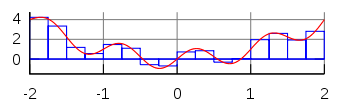
\includegraphics[width=7cm]{images/quadrature/int1}
b)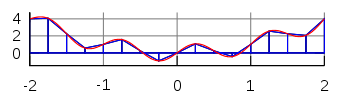
\includegraphics[width=7cm]{images/quadrature/int2}\\
The interval $[-2,2]$ is broken into 16 sub-intervals. The blue lines correspond to the 
approximation of the red curve by means of a) the midpoint rule,  b) the trapezoidal rule.
\end{center}

There are several algorithms for numerical integration (also commonly called 'numerical quadrature', or
simply 'quadrature') \index{quadrature}.
Interpolation with polynomials evaluated at equally spaced points in $[a,b]$
yields the Newton–Cotes formulas, of which the rectangle rule and the trapezoidal rule are examples. \index{Newton-Cotes}
If we allow the intervals between interpolation points to vary, we find another group of quadrature formulas, such as 
the Gauss(ian) quadrature formulas. \index{Gauss quadrature}
A Gaussian quadrature rule is typically more accurate than a Newton–Cotes rule, 
which requires the same number of function evaluations, if the integrand is smooth 
(i.e., if it is sufficiently differentiable).


An $n-$point Gaussian quadrature rule, named after Carl Friedrich Gauss, is a quadrature rule constructed
to yield an exact result for polynomials of degree $2n-1$ or less by a suitable choice of the points $x_i$
and weights $w_i$ for $i=1,\dots,n$.

The domain of integration for such a rule is conventionally taken as $[-1,1]$, so the rule is stated as
\[
\int_{-1}^{+1} f(x) dx = \sum_{i_q=1}^n w_{i_q} f(x_{i_q})
\]
In this formula the $x_{i_q}$ coordinate is 
the $i$-th root of the Legendre polynomial $P_n(x)$. \index{Legendre polynomial}

It is important to note that a Gaussian quadrature will only produce good results if the function $f(x)$
is well approximated by a polynomial function within the range $[-1,1]$.
As a consequence, the method is not, for example, suitable for functions with singularities.

\begin{center}
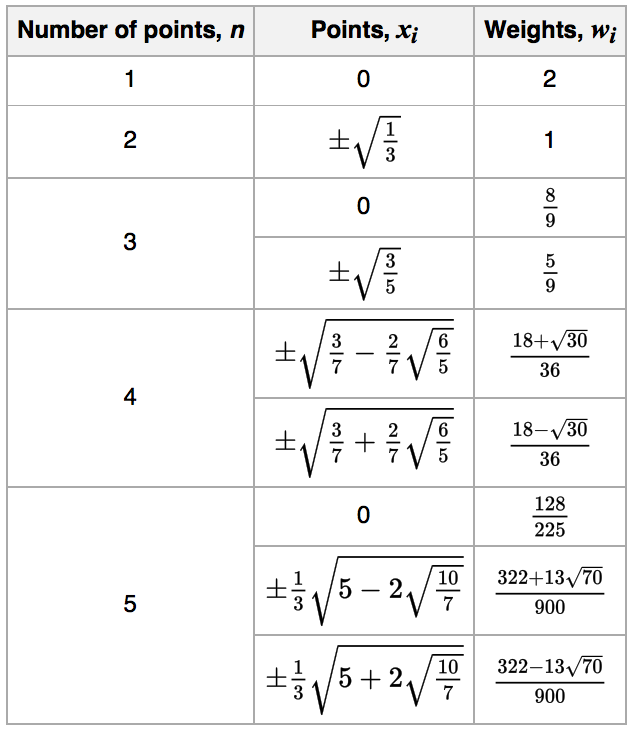
\includegraphics[width=5.cm]{images/quadrature/gq2}\\
Gauss-Legendre points and their weights.
\end{center}

\begin{tabular}{lllll}
\hline
n & $x_{iq}$ & $w_{iq}$ & $x_{iq}$ (approx) & $w_{iq}$ (approx) \\
\hline\hline
1 & 0 & 2 & 0 & 2 \\
\hline
2 & $\pm \sqrt{1/3}$ & 1  & $\pm$0.577350269189626 & 1 \\
\hline
3 & 0 & 8/9 & 0 & 0.888888888888889 \\
  & $\pm\sqrt{3/5}$  & 5/9  & $\pm$0.774596669241483 & 0.555555555555556 \\
\hline
4 & $\pm\sqrt{\frac{3}{7} - \frac{2}{7}\sqrt{6/5}}$  & $\frac{18+\sqrt{30}}{36}$ & $\pm$0.339981043584856 & 0.652145154862546 \\
  & $\pm\sqrt{\frac{3}{7} + \frac{2}{7}\sqrt{6/5}}$  & $\frac{18-\sqrt{30}}{36}$ & $\pm$0.861136311594053 & 0.347854845137454 \\
\hline
5 & 0 & 128/225 & 0 & 0.568888888888889 \\
  & $\pm\frac{1}{3}\sqrt{5-2\sqrt{\frac{10}{7}}}$  & $\frac{322+13\sqrt{70}}{900}$ & $\pm$0.538469310105683 & 0.478628670499366 \\
  & $\pm\frac{1}{3}\sqrt{5+2\sqrt{\frac{10}{7}}}$  & $\frac{322-13\sqrt{70}}{900}$ & $\pm$0.906179845938664 & 0.236926885056189 \\
\hline
6 & ?& ?& $\pm$0.23861 91860 83197 & 0.46791 39345 72691 \\
  & ?& ?& $\pm$0.66120 93864 66265 & 0.36076 15730 48139 \\
  & ?& ?& $\pm$0.93246 95142 03152 & 0.17132 44923 79170 \\
\hline
\end{tabular}



As shown in the above table, it can be shown that the weight values must fulfill the following condition:
\begin{equation}
\sum_{i_q} w_{i_q}=2 \label{gq23}
\end{equation}
and it is worth noting that all quadrature point coordinates are symmetrical around the origin.

Since most quadrature formula are only valid on a specific interval, we now must address the problem 
of their use outside of such intervals. The solution turns out to be quite simple: one 
must carry out a change of variables from the interval $[a,b]$ to $[-1,1]$.

We then consider the reduced coordinate $r\in[-1,1]$ such that 
\[
r=\frac{2}{b-a}(x-a)-1 
\]
This relationship can be reversed such that when $r$ is known, its equivalent coordinate 
$x\in[a,b]$ can be computed:
\[
x=\frac{b-a}{2}(1+r)+a
\]
From this it follows that
\[
dx=\frac{b-a}{2}dr
\]
and then 
\[
\int_a^b f(x) dx  = \frac{b-a}{2} \int_{-1}^{+1} f(r) dr \simeq 
\frac{b-a}{2} \sum_{i_q=1}^n w_{i_q} f(r_{i_q})
\]

%--------------------
\subsubsection{in 1D - examples}

\paragraph{example 1}

Since we know how to carry out any required change of variables, we choose for simplicity 
$a=-1$, $b=+1$.
Let us take for example $f(x)=\pi$. Then we can compute the integral of this function 
over the interval $[a,b]$ exactly:
\[
I=\int_{-1}^{+1} f(x) dx = \pi \int_{-1}^{+1}dx  = 2 \pi
\]
We can now use a Gauss-Legendre formula to compute this same integral:
\[
I_{gq}=\int_{-1}^{+1} f(x) dx 
= \sum_{i_q=1}^{n_q} w_{i_q} f(x_{i_q}) 
= \sum_{i_q=1}^{n_q} w_{i_q} \pi
= \pi \underbrace{\sum_{i_q=1}^{n_q} w_{i_q} }_{=2}
= 2 \pi
\]
where we have used the property of the weight values of Eq.(\ref{gq23}).
Since the actual number of points was never specified, this result is valid for all 
quadrature rules.


\paragraph{example 2}

Let us now take $f(x)=m x+ p$ and repeat the same exercise:
\[
I=\int_{-1}^{+1} f(x) dx = \int_{-1}^{+1} (mx+p) dx  =  [\frac{1}{2} m x^2 + p x ]_{-1}^{+1} =2p
\]
\[
I_{gq}=\int_{-1}^{+1} f(x) dx 
\!= \sum_{i_q=1}^{n_q} w_{i_q} f(x_{i_q}) 
\!= \sum_{i_q=1}^{n_q} w_{i_q} (m x_{i_q} + p)  
\!= m \underbrace{\sum_{i_q=1}^{n_q} w_{i_q} x_{i_q}}_{=0}  + p \underbrace{\sum_{i_q=1}^{n_q} w_{i_q}}_{=2}  = 2p
\]
since the quadrature points are symmetric w.r.t. to zero on the x-axis.
Once again the quadrature is able to compute the exact value of this integral: this makes sense since 
an $n$-point rule exactly integrates a $2n-1$ order polynomial such that a 1 point quadrature exactly 
integrates a first order polynomial like the one above.



\paragraph{example 3}

Let us now take $f(x)=x^2$. We have 
\[
I=\int_{-1}^{+1} f(x) dx = \int_{-1}^{+1} x^2 dx  =  [\frac{1}{3}x^3 ]_{-1}^{+1} =  \frac{2}{3} 
\]
and 
\[
I_{gq}=\int_{-1}^{+1} f(x) dx 
\!= \sum_{i_q=1}^{n_q} w_{i_q} f(x_{i_q}) 
\!= \sum_{i_q=1}^{n_q} w_{i_q} x_{i_q}^2 
\]

\begin{itemize}
\item $n_q=1$: $x_{iq}^{(1)}=0$, $w_{i_q}=2$. $I_{gq}=0$
\item $n_q=2$: $x_{q}^{(1)}=-1/\sqrt{3}$, $x_{q}^{(2)}=1/\sqrt{3}$, $w_{q}^{(1)}=w_{q}^{(2)}=1$. $I_{gq}=\frac{2}{3}$
\item It also works $\forall n_q>2$ !
\end{itemize}

%-----------------------------
\subsubsection{in 2D/3D - theory}


Let us now turn to a two-dimensional integral of the form
\[
I=\int_{-1}^{+1} \int_{-1}^{+1} f(x,y) dx dy
\]
The equivalent Gaussian quadrature writes:
\[
I_{gq}
\simeq \sum_{i_q=1}^{n_q}\sum_{j_q}^{n_q} f(x_{i_q},y_{j_q}) w_{i_q} w_{j_q}
\]

%----------------------------------------
\subsubsection{quadrature on triangles}

Quadrature rules for triangles can be found in Dunavant, 1985 \cite{duna85}.
The following ones are identical to those in the {\sl ip\_triangle.m} 
file of the MILAMIN code \cite{daks08}.

{\small
\[
\begin{array}{ccccccc}
\hline
&r_q & s_q & w_q \\ 
\hline\hline
iq=1& 1/3 & 1/3 & 1/2\\
\hline
iq=1 & 1/6 & 1/6 & 1/6 \\
iq=2 & 2/3 & 1/6 & 1/6 \\
iq=3 & 1/6 & 2/3 & 1/6 \\
\hline
iq=1&1/3 & 1/3 & -27/96\\
iq=2&0.6 & 0.2 &  25/96\\
iq=3&0.2 & 0.6 &  25/96\\
iq=4&0.2 & 0.2 &  25/96\\
\hline
iq=1& 1-2g_1 & g_1 & w_1/2  &  0.108103018168070 & 0.44594849091596  &   \\
iq=2& g_1 & 1-2g_1 & w_1/2  &  0.445948490915965 & 0.108103018168070 &   \\
iq=3& g_1 & g_1    & w_1/2  &  0.445948490915965 & 0.445948490915965 &   \\
iq=4& 1-2g_2 & g_2 & w_2/2  &  0.816847572980459 & 0.091576213509771 &   \\
iq=5& g_2 & 1-2g_2 & w_2/2  &  0.091576213509771 & 0.816847572980459 &   \\
iq=6& g_2 & g_2    & w_2/2  &  0.091576213509771 & 0.091576213509771 &   \\
\hline
iq=1&&&&0.091576213509771 &  0.091576213509771    &    0.109951743655322/2.0 \\ 
iq=2&&&&0.816847572980459 &  0.091576213509771    &    0.109951743655322/2.0 \\
iq=3&&&&0.091576213509771 &  0.816847572980459    &    0.109951743655322/2.0 \\
iq=4&&&&0.445948490915965 &  0.445948490915965    &    0.223381589678011/2.0 \\
iq=5&&&&0.108103018168070 &  0.445948490915965    &    0.223381589678011/2.0 \\
iq=6&&&&0.445948490915965 &  0.108103018168070    &    0.223381589678011/2.0 \\
\hline
iq=1 &&&&0.1012865073235 &  0.1012865073235  &     0.0629695902724 \\
iq=2 &&&&0.7974269853531 &  0.1012865073235  &     0.0629695902724 \\
iq=3 &&&&0.1012865073235 &  0.7974269853531  &     0.0629695902724 \\
iq=4 &&&&0.4701420641051 &  0.0597158717898  &     0.0661970763942 \\
iq=5 &&&&0.4701420641051 &  0.4701420641051  &     0.0661970763942 \\
iq=6 &&&&0.0597158717898 &  0.4701420641051  &     0.0661970763942 \\
iq=7 &&&&0.3333333333333 &  0.3333333333333  &     0.1125000000000 \\
\hline
iq=1&&&& 5.01426509658179E-01&  2.49286745170910E-01 &   5.83931378631895E-02 \\ 
iq=2&&&& 2.49286745170910E-01&  5.01426509658179E-01 &   5.83931378631895E-02 \\ 
iq=3&&&& 2.49286745170910E-01&  2.49286745170910E-01 &   5.83931378631895E-02 \\ 
iq=4&&&& 8.73821971016996E-01&  6.30890144915020E-02 &   2.54224531851035E-02 \\ 
iq=5&&&& 6.30890144915020E-02&  8.73821971016996E-01 &   2.54224531851035E-02 \\ 
iq=6&&&& 6.30890144915020E-02&  6.30890144915020E-02 &   2.54224531851035E-02 \\ 
iq=7&&&& 5.31450498448170E-02&  3.10352451033784E-01 &   4.14255378091870E-02 \\ 
iq=8&&&& 6.36502499121399E-01&  5.31450498448170E-02 &   4.14255378091870E-02 \\ 
iq=9&&&& 3.10352451033784E-01&  6.36502499121399E-01 &   4.14255378091870E-02 \\ 
iq=10&&&& 5.31450498448170E-02&  6.36502499121399E-01 &   4.14255378091870E-02 \\ 
iq=11&&&& 6.36502499121399E-01&  3.10352451033784E-01 &   4.14255378091870E-02 \\ 
iq=12&&&& 3.10352451033784E-01&  5.31450498448170E-02 &   4.14255378091870E-02 \\ 
\hline
\end{array}
\]
}

where
\[ 
g_1 = \left(8-\sqrt{10} + \sqrt{38-44\sqrt{2/5}}\right)/18
\qquad
g_2 = \left(8-\sqrt{10} - \sqrt{38-44\sqrt{2/5}}\right)/18
\]
\[
w_1 = \left(620+\sqrt{213125-53320\sqrt{10}}\right)/3720
\qquad
w_2 = \left(620-\sqrt{213125-53320\sqrt{10}}\right)/3720
\]


      


%----------------------------------------
\subsubsection{quadrature on tetrahedra}

\begin{remark}
In what follows the coefficients in the tables are not the reduced coordinates
of the quadratue points but the coefficients corresponding to the 4 nodes.
\end{remark}

Quadrature rules on tetrahedra take the form:
\[
\int\int\int_{el} f(x,y,z) dxdydz = V_{el} \sum_{iq=1}^{nqel} w_{iq} f(\xi^{iq}_1,\xi^{iq}_2,\xi^{iq}_3,\xi^{iq}_4) 
\]
or, that is to say:
\[
\int\int\int_{el} f(x,y,z) dxdydz = \sum_{iq=1}^{nqel} (w_{iq}V_{el}) f(\xi^{iq}_1,\xi^{iq}_2,\xi^{iq}_3,\xi^{iq}_4) 
\]
with in our case $V_{el}=1/6$.

In the literature it can be found that a one point quadrature is characterised by 
\[
w_{iq}=1 \quad\quad\quad \xi^{iq}_1=\xi^{iq}_2=\xi^{iq}_3=\xi^{iq}_4=0.25
\]
i.e, the coordinates of the single point are given by:
\[
x_{iq}=\sum_{i=1}^4 \xi_i^{iq} x_i = \frac{1}{4} (x_1+x_2+x_3+x_4)
\]
Same for $y$ and $z$ coordinates. 

A four-point quadrature rule is characterised by $w_{iq}=V_el*0.25=1/24\simeq 04166666666666667$ and 

\begin{tabular}{lcccc}
 & $\xi_1$ & $\xi_2$ & $\xi_3$ & $\xi_4$ \\
iq=1 & 0.585410196624969 & 0.138196601125011 & 0.138196601125011 & 0.138196601125011 \\
iq=2 & 0.138196601125011 & 0.585410196624969 & 0.138196601125011 & 0.138196601125011 \\
iq=3 & 0.138196601125011 & 0.138196601125011 & 0.585410196624969 & 0.138196601125011 \\
iq=4 & 0.138196601125011 & 0.138196601125011 & 0.138196601125011 & 0.585410196624969 \\
\end{tabular}

We then have:
\[
r_{iq}=\sum_{i=1}^4 \xi_i^{iq} x_i 
= (\xi_1^{iq},\xi_2^{iq},\xi_3^{iq},\xi_4^{iq})\cdot(r_1,r_2,r_3,r_4) 
= (\xi_1^{iq},\xi_2^{iq},\xi_3^{iq},\xi_4^{iq})\cdot(0,1,0,0) 
= \xi_2^{iq}
\]
\[
s_{iq}=\sum_{i=1}^4 \xi_i^{iq} y_i 
= (\xi_1^{iq},\xi_2^{iq},\xi_3^{iq},\xi_4^{iq})\cdot(s_1,s_2,s_3,s_4) 
= (\xi_1^{iq},\xi_2^{iq},\xi_3^{iq},\xi_4^{iq})\cdot(0,0,1,0) 
= \xi_3^{iq}
\]
\[
t_{iq}=\sum_{i=1}^4 \xi_i^{iq} z_i 
= (\xi_1^{iq},\xi_2^{iq},\xi_3^{iq},\xi_4^{iq})\cdot(t_1,t_2,t_3,t_4) 
= (\xi_1^{iq},\xi_2^{iq},\xi_3^{iq},\xi_4^{iq})\cdot(0,0,0,1) 
= \xi_4^{iq}
\]
Finally:

\[
\begin{array}{ccccc}
     & r_q & s_q & t_q  & w_q \\
iq=1 & 0.138196601125011 & 0.138196601125011 & 0.138196601125011 & 0.04166666666666667\\
iq=2 & 0.585410196624969 & 0.138196601125011 & 0.138196601125011 & 0.04166666666666667\\
iq=3 & 0.138196601125011 & 0.585410196624969 & 0.138196601125011 & 0.04166666666666667\\
iq=4 & 0.138196601125011 & 0.138196601125011 & 0.585410196624969 & 0.04166666666666667\\
\end{array}
\]






\subsection{The mesh}

\subsection{A bit of FE terminology}

We introduce here some terminology for efficient element descriptions \cite{grsa}:
\begin{itemize}
\item For triangles/tetrahedra, the designation 
$P_m \times P_n$ \index{$P_m \times P_n$}
means that each component of the velocity
is approximated by continuous piecewise \index{piecewise} complete Polynomials of degree $m$ and
pressure by continuous piecewise complete Polynomials of degree  $n$.
For example $P_2 \times P_1$ means 
\[
u \sim a_1 + a_2 x + a_3 y + a_4 xy + a_5 x^2 + a_6 y^2
\]
with similar approximations for $v$, and 
\[
p \sim b_1 + b_2x + b_3 y
\]
Both velocity and pressure are continuous across element boundaries, 
and each triangular element contains 6 velocity nodes and three pressure nodes.

\item For the same families, \index{$P_m \times P_{-n}$} 
$P_m \times P_{-n}$
is as above, except that pressure is approximated via 
piecewise {\sl discontinuous} polynomials of degree $n$. For instance, $P_2 \times P_{-1}$ is the same 
as $P_2P_1$ except that pressure is now an independent linear function in each element and therefore 
discontinuous at element boundaries.

\item For quadrilaterals/hexahedra, the designation 
\index{$Q_m \times Q_n$}  $Q_m \times Q_n$
means that each component of the velocity
is approximated by a continuous piecewise polynomial of degree $m$ {\sl in each direction} on the quadrilateral
and likewise for pressure, except that the polynomial is of degree $n$.
For instance,  $Q_2 \times Q_1$ \index{$Q_2 \times Q_1$} means
\[
u \sim a_1 + a_2 x + a_3 y + a_4 xy + a_5 x^2 + a_6 y^2 + a_7 x^2y + a_8 xy^2 + a_9 x^2y^2
\]
and 
\[
p \sim b_1 + b_2x + b_3 y + b_4 xy
\]
\item For these same families, $Q_m \times Q_{-n}$ is as above, except that the pressure approximation 
is not continuous at element boundaries. \index{$Q_m \times Q_{-n}$}

\item Again for the same families, \index{$Q_m \times P_{-n}$} $Q_m \times P_{-n}$
 indicates the same velocity approximation 
with a pressure approximation that is a discontinuous complete piecewise polynomial of degree $n$
(not of degree $n$ in each direction !)

\item The designation $P_m^+$ or $Q_m^+$ means that some sort of bubble function \index{bubble function}
was added to the polynomial approximation for the velocity. You may also find the term 'enriched element'
in the literature.

\item Finally, for $n=0$, we have piecewise-constant pressure, and we omit the minus sign for simplicity.
\end{itemize}

Another point which needs to be clarified is the use of so-called 'conforming elements' 
(or 'non-conforming elements'). \index{conforming element} \index{non-conforming element}
Following again \cite{grsa}, conforming velocity elements are those for which the basis functions for a subset 
of $H^1$ for the continuous problem (the first derivatives and their squares are integrable in $\Omega$).
For instance, the rotated $Q_1 \times P_0$ element of Rannacher and Turek (see section \ref{ncq1p0}) is such that 
the velocity is discontinous across element edges, so that the derivative does not exist there. Another
typical example of non-conforming element is the Crouzeix-Raviart element \cite{crra73}.

 




\subsection{Elements and basis functions in 1D}

%------------------------------------------
\subsubsection{Linear basis functions ($Q_1$)}
\index{$Q_1$}

Let $f(r)$ be a $C^1$ function on the interval $[-1:1]$ with $f(-1)=f_1$  and $f(1)=f_2$.
\begin{center}
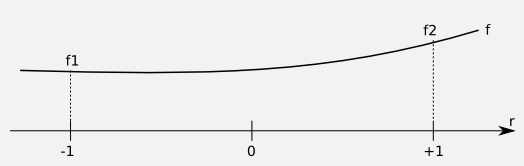
\includegraphics[width=8cm]{images/linshapefct.png}
\end{center}
Let us assume that the function $f(r)$ is to be approximated on $[-1,1]$ by the first order polynomial 
\begin{equation}
f(r)=a+br \label{eqquad1}
\end{equation}
Then it must fulfill
\begin{eqnarray}
f(r=-1)&=&a-b =f_1 \nonumber\\
f(r=+1)&=&a+b =f_2 \nonumber
\end{eqnarray}
This leads to  
\[
a=\frac{1}{2}(f_1+f_2)  
\quad\quad
b=\frac{1}{2}(-f_1+f_2)  
\]
and then replacing $a,b$ in Eq. (\ref{eqquad1}) by the above values on gets
\[
f(r) = \left[  \frac{1}{2}(1-r)\right] f_1 + \left[ \frac{1}{2}(1+r) \right] f_2
\]
or
\[
f(r)=\sum_{i=1}^2 N_i(r) f_1
\]
with
\begin{mdframed}[backgroundcolor=blue!5]
\begin{eqnarray}
N_1(r) &=& \frac{1}{2} (1-r) \nonumber\\
N_2(r) &=& \frac{1}{2} (1+r)
\end{eqnarray}
\end{mdframed}

%------------------------------------------
\subsubsection{Quadratic basis functions ($Q_2$)}
\index{$Q_2$}

Let $f(r)$ be a $C^1$ function on the interval $[-1:1]$ with $f(-1)=f_1$, $f(0)=f_2$ and $f(1)=f_3$.
\begin{center}
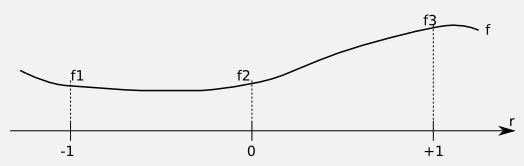
\includegraphics[width=8cm]{images/quadshapefct.png}
\end{center}

Let us assume that the function $f(r)$ is to be approximated on $[-1,1]$ by the second order polynomial
\begin{equation}
f(r)=a+br+cr^2 \label{eqquad}
\end{equation}
Then it must fulfill
\begin{eqnarray}
f(r=-1)&=&a-b+c = f_1 \nonumber\\
f(r=0) &=&a\quad\quad\quad\;     = f_2 \nonumber\\
f(r=+1)&=&a+b+c = f_3 \nonumber
\end{eqnarray}
This leads to
\[
a=f_2 
\quad
b=\frac{1}{2}(-f1+f3)
\quad
c=\frac{1}{2}(f_1+f_3-2f_2)
\]
and then replacing $a,b,c$ in Eq. (\ref{eqquad}) by the above values on gets
\[
f(r)=\left[\frac{1}{2}r(r-1)\right] f_1 + (1-r^2) f_2 + \left[\frac{1}{2}r(r+1)\right] f_3
\]
or,
\[
f(r) = \sum_{i=1}^3 N_i(r) f_i
\]
with
\begin{mdframed}[backgroundcolor=blue!5]
\begin{eqnarray}
N_1(r) &=& \frac{1}{2}r(r-1) \nonumber\\
N_2(r) &=& (1-r^2) \nonumber\\ 
N_3(r) &=& \frac{1}{2}r(r+1) 
\end{eqnarray}
\end{mdframed}



%------------------------------------------
\subsubsection{Cubic basis functions ($Q_3$)}
\index{$Q_3$}

The 1D basis polynomial is given by
\[
f(r)=a+br+cr^2+dr^3
\]
with the nodes at position -1,-1/3, +1/3 and +1.

\begin{eqnarray}
f(-1)   &=& a-b+c-d = f_1 \nonumber\\
f(-1/3) &=& a-\frac{b}{3}+\frac{c}{9}-\frac{d}{27} = f_2 \nonumber\\
f(+1/3) &=& a-\frac{b}{3}+\frac{c}{9}-\frac{d}{27} = f_3 \nonumber\\
f(+1)   &=& a+b+c+d = f_4 \nonumber
\end{eqnarray}

Adding the first and fourth equation and the second and third, one arrives at
\[
f_1+f_4 = 2a+2c \quad\quad\quad f_2+f_3=2a+\frac{2c}{9}
\]
and finally:
\[
a=\frac{1}{16} \left( -f_1 + 9f_2 + 9f_3 - f_4  \right)
\]
\[
c=\frac{9}{16}\left(f_1-f_2-f_3+f_4\right)
\]
Combining the original 4 equations in a different way yields
\[
2b+2d=f_4-f_1 
\quad\quad\quad
\frac{2b}{3} + \frac{2d}{27} = f_3-f_2
\]
so that
\[
b=\frac{1}{16} \left( f_1 - 27f_2 + 27f_3 -f_4   \right)
\]
\[
d=\frac{9}{16} \left( -f_1 + 3f_2 - 3f_3 + f_4 \right)
\]
Finally,

\begin{eqnarray}
f(r) 
&=& a+b+cr^2+dr^3 \nonumber\\
&=& \frac{1}{16} (-1+  r +9r^2 - 9r^3 )f_1 \nonumber\\ 
&+& \frac{1}{16} ( 9-27r -9r^2 +27r^3 )f_2 \nonumber\\ 
&+& \frac{1}{16} ( 9+27r -9r^2 -27r^3 )f_3 \nonumber\\ 
&+& \frac{1}{16} (-1-  r +9r^2 + 9r^3 )f_4 \nonumber\\ 
&=& \sum_{i=1}^4 N_i(r) f_i \nonumber
\end{eqnarray}
where
\begin{mdframed}[backgroundcolor=blue!5]
\begin{eqnarray}
N_1&=& \frac{1}{16} (-1+  r+9r^2- 9r^3 ) \nonumber\\ 
N_2&=& \frac{1}{16} ( 9-27r-9r^2+27r^3 ) \nonumber\\ 
N_3&=& \frac{1}{16} ( 9+27r-9r^2-27r^3 ) \nonumber\\ 
N_4&=& \frac{1}{16} (-1-  r+9r^2+ 9r^3 ) \nonumber
\end{eqnarray}
\end{mdframed}
Verification:

\begin{itemize}
\item
Let us assume $f(r)=C$, then
\[
\hat{f}(r) = \sum N_i(r) f_i = \sum_i N_i C = C \sum_i N_i  = C
\]
so that a constant function is exactly reproduced, as expected.

\item
Let us assume $f(r)= r$, then $f_1=-1$, $f_2=-1/3$, $f_3=1/3$ and $f_4=+1$. We then have
\begin{eqnarray}
\hat{f}(r) 
&=& \sum N_i(r) f_i  \nonumber\\
&=& - N_1(r) -\frac{1}{3}N_2(r) + \frac{1}{3}N_3(r)  + N_4(r) \nonumber\\
&=& [-(-1+  r+9r^2- 9r^3 ) \nn\\
&&- \frac{1}{3} ( 9-27r-9r^2-27r^3 ) \nn\\
&&+ \frac{1}{3} ( 9+27r-9r^2+27r^3 ) \nn\\
&&+ (-1-  r+9r^2+ 9r^3 )]/16 \nonumber\\
&=& [-r +9r + 9r -r]/16  + ... 0 ... \nonumber\\
&=& r   
\end{eqnarray}

\end{itemize}


The basis functions derivative are given by
\begin{mdframed}[backgroundcolor=blue!5]
\begin{eqnarray}
 \frac{\partial N_1}{\partial r}&=& \frac{1}{16}  (  1 +18r - 27r^2 ) \nonumber\\ 
 \frac{\partial N_2}{\partial r}&=& \frac{1}{16}  (-27 -18r + 81r^2 ) \nonumber\\ 
 \frac{\partial N_3}{\partial r}&=& \frac{1}{16}  (+27 -18r - 81r^2 ) \nonumber\\ 
 \frac{\partial N_4}{\partial r}&=& \frac{1}{16}  ( -1 +18r + 27r^2 ) \nonumber
\end{eqnarray}
\end{mdframed}
Verification:

\begin{itemize}
\item
Let us assume $f(r)=C$, then
\begin{eqnarray}
\frac{\partial \hat{f}}{\partial r} 
&=& \sum_i \frac{\partial N_i}{\partial r} f_i  \nonumber\\
&=&  C \sum_i \frac{\partial N_i}{\partial r}  \nonumber\\
&=& \frac{C}{16} [  (  1 +18r - 27r^2 ) \nn\\
&&+ (-27 -18r + 81r^2 )  \nn\\
&&+  (+27 -18r - 81r^2 ) \nn\\
&&+ ( -1 +18r + 27r^2 ) ]  \nonumber\\
&=& 0 \nonumber
\end{eqnarray}

\item
Let us assume $f(r)= r$, then $f_1=-1$, $f_2=-1/3$, $f_3=1/3$ and $f_4=+1$. We then have
\begin{eqnarray}
\frac{\partial \hat{f}}{\partial r} 
&=& \sum_i \frac{\partial N_i}{\partial r} f_i  \nonumber\\
&=& \frac{1}{16} [  -(  1 +18r - 27r^2 ) \nn\\ 
&& -\frac{1}{3} (-27 -18r + 81r^2 )  \nn\\
&& +\frac{1}{3}  (+27 -18r - 81r^2 ) \nn\\
&& + ( -1 +18r + 27r^2 ) ]  \nonumber\\
&=& \frac{1}{16} [-2 + 18 + 54r^2 - 54r^2] \nonumber\\
&=& 1 \nonumber
\end{eqnarray}

\end{itemize}





\subsection{Elements and basis functions in 2D}
Let us for a moment consider a single quadrilateral element in the $xy$-plane, 
as shown on the following figure:
\begin{center}
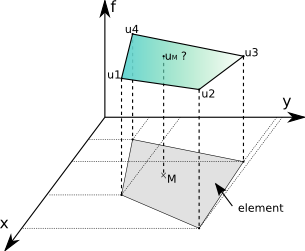
\includegraphics[width=5.8cm]{images/shape.png}
\end{center}
Let us assume that we know the values of a given field $u$ at the vertices.
For a given point $M$ inside the element in the plane, what is the value of the 
field $u$ at this point?
It makes sense to postulate that $u_M=u(x_M,y_M)$ will be given  by 
\[
u_M= \phi(u_1,u_2,u_3,u_4,x_M,y_M) 
\]
where $\phi$ is a function to be determined. Although $\phi$ is not unique, we can 
decide to express the value $u_M$ as a weighed sum of the values at the vertices $u_i$.
One option could be to assign all four vertices the same weight, say $1/4$ so that 
$u_M=(u_1+u_2+u_3+u_4)/4$, i.e. $u_M$ is simply given by the arithmetic mean 
of the vertices values. This approach suffers from a major drawback as it does
not use the location of point $M$ inside the element. For instance, when 
$(x_M,y_M) \rightarrow (x_2,y_2)$ we expect $u_M \rightarrow u_2$.

In light of this, we could now assume that the weights would depend on the position 
of $M$ in a continuous fashion:
\[
u(x_M,y_M) = \sum_{i=1}^4 N_i(x_M,y_M)\;  u_i
\]
where the $N_i$ are continous ("well behaved") functions which have the property:
\[
N_i(x_j,y_j)=\delta_{ij}
\]
or, in other words: 
\begin{eqnarray}
N_3(x_1,y_1) &=& 0 \\
N_3(x_2,y_2) &=& 0 \\
N_3(x_3,y_3) &=& 1 \\
N_3(x_4,y_4) &=& 0 
\end{eqnarray}
The functions $N_i$ are commonly called basis functions. \index{basis functions}

Omitting the $M$ subscripts for any point inside the element, the velocity components $u$
and $v$ are given by:
\[
u(x,y) = \sum_{i=1}^4 N_i(x,y)\;  u_i
\]
\[
v(x,y) = \sum_{i=1}^4 N_i(x,y)\;  v_i
\]
Rather interestingly, one can now easily compute velocity gradients (and therefore the 
strain rate tensor) since we have assumed the basis functions to be "well behaved" 
(in this case differentiable):
\begin{eqnarray}
\dot{\epsilon}_{xx}(x,y) &=& \frac{\partial u}{\partial x} = \sum_{i=1}^4 \frac{\partial N_i}{\partial x}\;  u_i \\
\dot{\epsilon}_{yy}(x,y) &=& \frac{\partial v}{\partial y} = \sum_{i=1}^4 \frac{\partial N_i}{\partial y}\;  v_i \\
\dot{\epsilon}_{xy}(x,y) &=& \frac{1}{2}\frac{\partial u}{\partial y} 
+ \frac{1}{2}\frac{\partial v}{\partial x} 
= \frac{1}{2}\sum_{i=1}^4 \frac{\partial N_i}{\partial y}\;  u_i
+ \frac{1}{2}\sum_{i=1}^4 \frac{\partial N_i}{\partial x}\;  v_i
\end{eqnarray}
How we actually obtain the exact form of the basis functions is explained in the coming section.


%%%%%%%%%%%%%%%%%%%%%%%%%%%%%%%%%%%%5
\subsubsection{The $Q_1$ space}



\begin{center}
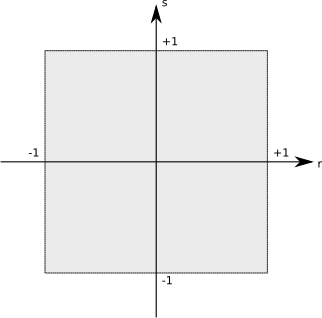
\includegraphics[height=3.5cm]{images/element_rs.png}
\end{center}

\begin{eqnarray}
N_1(r,s)&=&0.25(1-r)(1-s) \nonumber\\
N_2(r,s)&=&0.25(1+r)(1-s) \nonumber\\
N_3(r,s)&=&0.25(1+r)(1+s) \nonumber\\
N_4(r,s)&=&0.25(1-r)(1+s) \nonumber
\end{eqnarray}

\begin{eqnarray}
\frac{\partial N_1}{\partial r}(r,s)&=& - 0.25(1-s) \nonumber\\
\frac{\partial N_2}{\partial r}(r,s)&=& + 0.25(1-s) \nonumber\\
\frac{\partial N_3}{\partial r}(r,s)&=& + 0.25(1+s) \nonumber\\
\frac{\partial N_4}{\partial r}(r,s)&=& - 0.25(1+s) \nonumber
\end{eqnarray}

\begin{eqnarray}
\frac{\partial N_1}{\partial s}(r,s)&=& - 0.25(1-r) \nonumber\\
\frac{\partial N_2}{\partial s}(r,s)&=& - 0.25(1+r) \nonumber\\
\frac{\partial N_3}{\partial s}(r,s)&=& + 0.25(1+r) \nonumber\\
\frac{\partial N_4}{\partial s}(r,s)&=& + 0.25(1-r) \nonumber
\end{eqnarray}



\newpage %------------------------------------------------------------------
%---------------------------------------------------------------------------
\section{Solving the Stokes equations with the FEM} %-----------------------
%6.3 of donea and huerta

In the case of an incompressible flow, we have seen that the continuity (mass conservation)
equation takes the simple form ${\vec \nabla}\cdot{\vec \upnu}=0$. In other words flow takes place 
under the constraint that the divergence of its velocity field is exactly zero eveywhere 
(solenoidal constraint), i.e. it is divergence free. 
\index{general}{Divergence-free Flow} 
\index{general}{Solenoidal Field}

We see that the pressure in the momentum equation is then a degree of freedom which is needed 
to satisfy the incompressibilty constraint (and it is not related to any constitutive equation)
\cite{dohu03}. In other words the pressure is acting as a Lagrange multiplier of the incompressibility
constraint. 

Various approaches have been proposed in the literature to deal with the 
incompressibility constraint but we will only focus on the penalty method 
(section \ref{sec:penalty}) and the so-called mixed finite element method
\ref{sec:mixed}.
 %----------------------------------------------------
\subsection{strong and weak forms} \begin{flushright} {\tiny {\color{gray} strongweak.tex}} \end{flushright}

\index{general}{strong form} 

The strong form consists of the governing equation and the boundary conditions, i.e. 
the mass, momentum and energy conservation equations supplemented with Dirichlet and/or Neumann
boundary conditions on (parts of) the boundary.


\index{general}{weak form}
To develop the finite element formulation, the partial differential equations 
must be restated in an integral form called the weak form. In essence the PDEs are 
first multiplied by an arbitrary function and integrated over the domain.

 

 %---------------------
\subsection{The penalty approach} \label{sec_penalty}

\index{penalty formulation}

In order to impose the incompressibility constraint, two widely used procedures are available, namely the 
Lagrange multiplier method and the penalty method \cite{bathe82,hugh}. The latter is implemented in {\sc elefant}, which allows for the elimination of the pressure variable from the momentum equation (resulting in a reduction of the matrix size).%, based on a relaxation of the incompressibility constraint. 

Mathematical details on the origin and validity of the penalty approach applied to the Stokes problem can for instance be found in  \cite{cuss86}, \cite{redd82} or \cite{gunz89}.

The penalty formulation of the mass conservation equation is based on a relaxation of the incompressibility constraint and writes 
\begin{equation}
{\vec \nabla}\cdot {\vec \upnu} + \frac{p}{\lambda} = 0 \label{penal}
\end{equation}
where $\lambda$ is the penalty parameter, that can be interpreted (and has the same dimension) as a bulk viscosity. It is 
equivalent to say that the material is weakly compressible. It can be shown that if one chooses $\lambda$ to be a 
sufficiently large number, the continuity equation $ {\vec \nabla}\cdot {\vec \upnu} = 0$ will be approximately satisfied in the finite element solution. The value of $\lambda$ is often recommended to be 6 to 7 orders of magnitude larger than the shear viscosity \cite{dohu03,hulb79}.

%Note that Eq. (\ref{penal}) does not form the basis of the penalty method (as often implied) for the Stokes equation but is a consequence of minimising a modified functional of the problem under certain assumptions \cite{redd82}. 

Equation (\ref{penal}) can be used to eliminate the pressure in Eq. (\ref{mce2}) so that the mass and momentum conservation equations fuse to become :
\begin{equation}
{\vec \nabla}\cdot ( 2 \eta \dot\varepsilon({\vec \upnu})) 
+ \lambda {\vec \nabla} ({\vec \nabla }\cdot {\vec \upnu}) = \rho {\bm g} = 0 \label{peneq}
\end{equation}

\cite{mahu78} have established the equivalence for incompressible problems between the reduced integration
of the penalty term and a mixed Finite Element approach if the pressure nodes coincide with the integration points of the reduced rule.

In the end, the elimination of the pressure unknown in the Stokes equations
replaces the original saddle-point Stokes problem \cite{begl05} by an elliptical problem, 
which leads to a symmetric positive definite (SPD) FEM matrix. 
%Such systems always admit a square root triangular matrix (the Cholesky factor, L) and can be solved, once L has been computed (Cholesky factorization), by 2 triangular matrix solves (upper and lower back-substitutions). 
This is the major benefit of the penalized approach 
over the full indefinite solver with the velocity-pressure variables. Indeed, the SPD character of the matrix lends itself 
to efficient solving stragegies and is less memory-demanding since it is sufficient to store only the upper half of the matrix including the diagonal
\cite{gova}
.
\improvement{list codes which use this approach}


The stress tensor ${\bm \sigma}$ is symmetric ({\it i.e.} $\sigma_{ij}=\sigma_{ji}$). For simplicity
I will now focus on a Stokes flow in two dimensions. 

Since the penalty formulation is only valid for incompressible flows, then 
$\dot{\bm \epsilon}=\dot{\bm \epsilon}^d$ so that the $d$ superscript is ommitted in what follows.
The stress tensor can also be cast in vector format:
\begin{eqnarray}
\left(
\begin{array}{c}
\sigma_{xx}\\
\sigma_{yy}\\
\sigma_{xy}\\
\end{array}
\right)
&=&
\left(
\begin{array}{c}
-p \\
-p\\
0
\end{array}
\right)
+2 \eta
\left(
\begin{array}{c}
\dot{\epsilon}_{xx}\\
\dot{\epsilon}_{yy}\\
\dot{\epsilon}_{xy}\\
\end{array}
\right)
\nonumber\\
&=&
\lambda
\left(
\begin{array}{c}
\dot{\epsilon}_{xx} + \dot{\epsilon}_{yy}\\
\dot{\epsilon}_{xx} + \dot{\epsilon}_{yy}\\
0
\end{array}
\right)
+2 \eta
\left(
\begin{array}{c}
\dot{\epsilon}_{xx}\\
\dot{\epsilon}_{yy}\\
\dot{\epsilon}_{xy}\\
\end{array}
\right)\nonumber\\
&=&
\left[
\lambda
\underbrace{
\left(
\begin{array}{ccc}
1 & 1 & 0\\
1 & 1 & 0\\
0 & 0 & 0\\
\end{array}
\right)}_{\bm K}
+ \eta
\underbrace{
\left(
\begin{array}{ccc}
2 & 0 & 0 \\
0 & 2 & 0 \\
0 & 0 & 1 \\
\end{array}
\right)
}_{\bm C}
\right]
\cdot
\left(
\begin{array}{c}
\frac{\partial u}{\partial x} \\ \\
\frac{\partial v}{\partial y} \\ \\
\frac{\partial u}{\partial y} + \frac{\partial v}{\partial x} \\
\end{array}
\right) \nonumber
\end{eqnarray}


Remember that
\[
\frac{\partial u}{\partial x} = \sum_{i=1}^4 \frac{\partial N_i}{\partial x}\;  u_i 
\quad\quad
\frac{\partial v}{\partial y} = \sum_{i=1}^4 \frac{\partial N_i}{\partial y}\;  v_i 
\]

\[
\frac{\partial u}{\partial y} 
+\frac{\partial v}{\partial x} 
= \sum_{i=1}^4 \frac{\partial N_i}{\partial y}\;  u_i
+ \sum_{i=1}^4 \frac{\partial N_i}{\partial x}\;  v_i
\]

so that
\[
\left(
\begin{array}{c}
\frac{\partial u}{\partial x} \\ \\
\frac{\partial v}{\partial y} \\ \\
\frac{\partial u}{\partial y} + \frac{\partial v}{\partial x} \\
\end{array}
\right)
=
\underbrace{
\left(
\begin{array}{cccccccc}
\frac{\partial N_1}{\partial x} & 0 & \frac{\partial N_2}{\partial x} & 0 & \frac{\partial N_3}{\partial x} & 0 & \frac{\partial N_4}{\partial x} & 0 \\  \\
0 & \frac{\partial N_1}{\partial y} & 0 & \frac{\partial N_2}{\partial y} & 0 & \frac{\partial N_3}{\partial y} & 0 & \frac{\partial N_4}{\partial y}  \\ \\
\frac{\partial N_1}{\partial y} &  \frac{\partial N_1}{\partial x} &  \frac{\partial N_2}{\partial y} &  \frac{\partial N_2}{\partial x} & 
\frac{\partial N_3}{\partial y} &  \frac{\partial N_3}{\partial x} &  \frac{\partial N_3}{\partial y} &  \frac{\partial N_4}{\partial x}  
\end{array}
\right)
}_{\bm B}
\cdot
\underbrace{
\left(
\begin{array}{c}
u1 \\ v1 \\ u2 \\ v2 \\ u3 \\ v3 \\ u4 \\ v4
\end{array}
\right)
}_{\bm V}
\]
Finally,
\[
\vec{\sigma}=
\left(
\begin{array}{c}
\sigma_{xx}\\
\sigma_{yy}\\
\sigma_{xy}\\
\end{array}
\right)
=
(\lambda {\bm K} +  \eta {\bm C} )\cdot {\bm B} \cdot {\bm V}
\]

\index{weak form}
We will now establish the weak form of the momentum conservation equation. 
We start again from 
\[
{\vec \nabla}\cdot {\bm \sigma} + {\vec b} = {\vec 0} 
\]
For the $N_i$'s 'regular enough', we can write:
\[
\int_{\Omega_e} N_i {\vec \nabla}\cdot {\bm \sigma} d\Omega + \int_{\Omega_e} N_i  {\bm b} d\Omega =0
\]
We can integrate by parts and drop the surface term\footnote{We will come back to this at a later stage}:
\[
\int_{\Omega_e} {\vec \nabla } N_i \cdot {\bm \sigma} d\Omega = \int_{\Omega_e} N_i  {\bm b} d\Omega 
\]
or, 
\[
\int_{\Omega_e} 
\left(
\begin{array}{ccc}
\frac{\partial N_i}{\partial x} & 0 & \frac{\partial N_i}{\partial y} \\  \\
0 & \frac{\partial N_i}{\partial y} &  \frac{\partial N_i}{\partial x}  
\end{array}
\right)
\cdot
\left(
\begin{array}{c}
\sigma_{xx}\\
\sigma_{yy}\\
\sigma_{xy}\\
\end{array}
\right)
d\Omega = \int_{\Omega_e} N_i {\bm b} d\Omega 
\]
Let $i=1,2,3,4$ and stack the resulting four equations on top of one another. 
\begin{eqnarray}
\int_{\Omega_e} 
\left(
\begin{array}{ccc}
\frac{\partial N_1}{\partial x} & 0 & \frac{\partial N_1}{\partial y} \\  \\
0 & \frac{\partial N_1}{\partial y} &  \frac{\partial N_1}{\partial x}  
\end{array}
\right)
\cdot
\left(
\begin{array}{c}
\sigma_{xx}\\
\sigma_{yy}\\
\sigma_{xy}\\
\end{array}
\right)
d\Omega &=& \int_{\Omega_e} N_1 
\left(
\begin{array}{c}
b_x \\ b_y
\end{array}
\right)
 d\Omega \\
\int_{\Omega_e} 
\left(
\begin{array}{ccc}
\frac{\partial N_2}{\partial x} & 0 & \frac{\partial N_2}{\partial y} \\  \\
0 & \frac{\partial N_2}{\partial y} &  \frac{\partial N_2}{\partial x}  
\end{array}
\right)
\cdot
\left(
\begin{array}{c}
\sigma_{xx}\\
\sigma_{yy}\\
\sigma_{xy}\\
\end{array}
\right)
d\Omega &=& \int_{\Omega_e} N_i 
\left(
\begin{array}{c}
b_x \\ b_y
\end{array}
\right)
d\Omega \\
\int_{\Omega_e} 
\left(
\begin{array}{ccc}
\frac{\partial N_3}{\partial x} & 0 & \frac{\partial N_3}{\partial y} \\  \\
0 & \frac{\partial N_3}{\partial y} &  \frac{\partial N_3}{\partial x}  
\end{array}
\right)
\cdot
\left(
\begin{array}{c}
\sigma_{xx}\\
\sigma_{yy}\\
\sigma_{xy}\\
\end{array}
\right)
d\Omega &=& \int_{\Omega_e} N_3 
\left(
\begin{array}{c}
b_x \\ b_y
\end{array}
\right)
d\Omega \\
\int_{\Omega_e} 
\left(
\begin{array}{ccc}
\frac{\partial N_4}{\partial x} & 0 & \frac{\partial N_4}{\partial y} \\  \\
0 & \frac{\partial N_4}{\partial y} &  \frac{\partial N_4}{\partial x}  
\end{array}
\right)
\cdot
\left(
\begin{array}{c}
\sigma_{xx}\\
\sigma_{yy}\\
\sigma_{xy}\\
\end{array}
\right)
d\Omega &=& \int_{\Omega_e} N_4 
\left(
\begin{array}{c}
b_x \\ b_y
\end{array}
\right)
d\Omega 
\end{eqnarray}
We easily recognize ${\bm B}^T$ inside the integrals!
Let us define 
\[
{\bm N}_b^T=(N_1 b_x , N_1 b_y, ... N_4 b_x, N_4 b_y)
\]
then we can write
\[
\int_{\Omega_e} {\bm B}^T \cdot 
\left(
\begin{array}{c}
\sigma_{xx}\\
\sigma_{yy}\\
\sigma_{xy}\\
\end{array}
\right)
d\Omega
=
\int_{\Omega_e} {\bm N}_b d\Omega 
\]
and finally:
\[
\int_{\Omega_e} {\bm B}^T \cdot [ \lambda {\bm K} + \eta {\bm C} ] \cdot {\bm B} \cdot {\bm V} d\Omega
=
\int_{\Omega_e} {\bm N}_b d\Omega 
\]
Since $V$ contains the velocities at the corners, it does not depend on the $x$ or $y$ coordinates
so it can be taking outside of the integral:
\[
\underbrace{
\left(\int_{\Omega_e} {\bm B}^T \cdot [ \lambda {\bm K} + \eta {\bm C} ] \cdot {\bm B} d\Omega \right) 
}_{A_{el}(8 \times 8)}
\cdot 
\underbrace{
{\bm V}
}_{(8x1)}
=
\underbrace{
\int_{\Omega_e} {\bm N}_b d\Omega 
}_{B_{el} (8\times 1)}
\]
or, 
\[
\left[
\underbrace{
\left(\int_{\Omega_e} \lambda {\bm B}^T \cdot {\bm K} \cdot {\bm B} d\Omega \right) 
}_{A_{el}^\lambda(8 \times 8)}
+
\underbrace{
\left(\int_{\Omega_e}  \eta {\bm B}^T \cdot {\bm C}  \cdot {\bm B} d\Omega \right) 
}_{A_{el}^\eta(8 \times 8)}
\right]
\cdot 
\underbrace{
{\bm V}
}_{(8x1)}
=
\underbrace{
\int_{\Omega_e} {\bm N}_b d\Omega 
}_{B_{el} (8\times 1)}
\]

INTEGRATION - MAPPING 

reduced integration \cite{hulb79}

\begin{enumerate}

\item partition domain $\Omega$ into elements $\Omega_e$, $e=1, ... n_{el}$.


\item loop over elements and for each element compute ${\bm A}_{el}$, ${\bm B}_{el}$ \\
\begin{center}
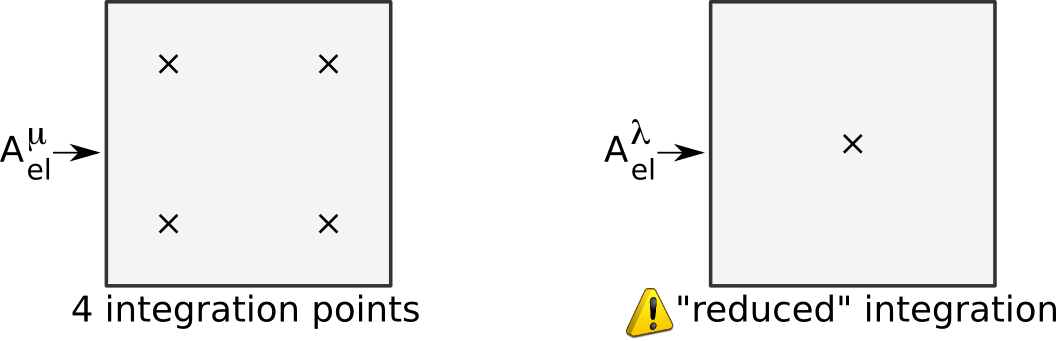
\includegraphics[width=5.5cm]{images/integration.png}
\end{center}

%
\includegraphics[width=0.5cm]{images/warning.png}
%4-point integration for ${\bm A}_{el}^\mu$, 1-point integration for ${\bm A}_{el}^\lambda$


\item a node belongs to several elements\\
      $\rightarrow$ need to assemble ${\bm A}_{el}$ and ${\bm B}_{el}$ in ${\bm A}$, ${\bm B}$

\item apply boundary conditions

\item solve system: ${\bm x}= {\bm A}^{-1} \cdot {\bm B}$
\item visualise/analyse ${\bm x}$
\end{enumerate}
 %-------------------------
\subsection{The mixed FEM} \index{general}{Mixed Formulation}
\begin{flushright} {\tiny {\color{gray} mixed.tex}} \end{flushright}

\subsubsection{In three dimensions}

The FEM formulation of the Stokes equation is quite complex so 
we simplify things as much as possible for now by 
assuming the flow to be \underline{incompressible}, 
\underline{isoviscous} and \underline{isothermal}. 

The methodology to derive the discretised equations of the mixed system is 
quite similar to the one we have used in the case of the penalty formulation.
The big difference comes from the fact that we are now solving for both 
velocity and pressure at the same time, and that we therefore must solve 
the mass and momentum conservation equations together.
As before, velocity inside an element is given by 
\begin{equation}
{\vec \upnu}^h({\vec r})=\sum_{i=1}^{m_v} \bN_i^\upnu({\vec r})\;  {\vec \upnu}_i
\label{mixed01}
\end{equation}
where $N_i^{\upnu}$ are the polynomial basis functions for the velocity,
and the summation runs over the $m_v$ velocity nodes composing the element.
A similar expression is used for pressure:
\begin{equation}
p^h({\vec r})=\sum_{i=1}^{m_p} \bN_i^p({\vec r}) \; p_i
\label{mixed02}
\end{equation}
Note that the velocity is a vector of size while pressure (and temperature)
is a scalar. There are then $ndof_v$ velocity degrees of freedom per node
and $ndof_p$ pressure degrees of freedom.
It is also very important to remember that the numbers of 
velocity nodes and pressure nodes for a given element 
are more often than not different and that velocity and pressure
nodes need not be colocated. Indeed, unless 
so-called 'stabilised elements' are used, we have $m_v>m_p$, which 
means that the polynomial order of the velocity field is higher than 
the polynomial order of the pressure field (usually by value 1).

Other notations will be sometimes used for Eqs.~\eqref{mixed01} and \eqref{mixed02}:
\begin{equation}
u^h({\vec r}) = \vec{\bN}^\upnu \cdot \vec{u}
\quad\quad\quad\quad
v^h({\vec r}) = \vec{\bN}^\upnu \cdot \vec{v}
\quad\quad\quad\quad
w^h({\vec r}) = \vec{\bN}^\upnu \cdot \vec{w}
\quad\quad\quad\quad
p^h({\vec r}) = \vec{\bN}^p \cdot \vec{p}
\end{equation} 
where ${\vec \upnu}=(u,v,w)$ and $\vec{\bN}^\upnu$ is the vector containing 
all basis functions evaluated at location ${\vec r}$:
\begin{eqnarray}
\vec{\bN}^v &=& \left( \bN_1^\upnu({\vec r}),  \bN_2^\upnu({\vec r}),  
\bN_3^\upnu({\vec r}), \dots  \bN_{m_v}^\upnu({\vec r}) \right) \\
\vec{\bN}^p &=& \left( \bN_1^p({\vec r}),  \bN_2^p({\vec r}),  
\bN_3^p({\vec r}), \dots  \bN_{m_p}^p({\vec r}) \right)
\end{eqnarray}
and with 
\begin{eqnarray}
\vec{u} &=& \left( u_1,  u_2,  u_3, \dots  u_{m_v} \right) \\
\vec{v} &=& \left( v_1,  v_2,  v_3, \dots  v_{m_v} \right) \\
\vec{w} &=& \left( w_1,  w_2,  w_3, \dots  w_{m_v} \right) \\
\vec{p} &=& \left( p_1,  p_2,  p_3, \dots  p_{m_p} \right) 
\end{eqnarray}
We will now establish the weak form of the momentum conservation equation. 
We start again from 
\begin{eqnarray}
{\vec \nabla}\cdot {\bm \sigma} + {\vec b} &=& {\vec 0} \\
{\vec \nabla}\cdot {\vec v} &=& 0
\end{eqnarray}
For the $\bN_i^\upnu$'s and $\bN_i^p$ 'regular enough', we can write:
\begin{eqnarray}
\int_{\Omega_e} \bN_i^\upnu {\vec \nabla}\cdot {\bm \sigma}\;  dV
+ \int_{\Omega_e} \bN_i^\upnu  {\vec b} \; dV
&=& \vec 0 \\
\int_{\Omega_e} \bN_i^p {\vec \nabla}\cdot {\vec v} \; dV &=& 0
\end{eqnarray}
We can integrate by parts and drop the surface term\footnote{We will come back to this at a later stage}:
\begin{eqnarray}
\int_{\Omega_e} {\vec \nabla } \bN_i^\upnu \cdot {\bm \sigma} dV
&=& \int_{\Omega_e} \bN_i^\upnu  {\vec b} \; dV \\
\int_{\Omega_e} \bN_i^p {\vec \nabla}\cdot {\vec v} \; dV &=& 0
\end{eqnarray}
or, 
\begin{equation}
\int_{\Omega_e} 
\left(
\begin{array}{cccccc}
\frac{\partial \bN_i^\upnu}{\partial x} & 0 & 0& 
\frac{\partial \bN_i^\upnu}{\partial y} & 
\frac{\partial \bN_i^\upnu}{\partial z} & 0\\  \\
0 & \frac{\partial \bN_i^\upnu}{\partial y} & 0  & 
\frac{\partial \bN_i^\upnu}{\partial x}  & 0 &
\frac{\partial \bN_i^\upnu}{\partial z}  \\ \\
0 & 0 & \frac{\partial \bN_i^\upnu}{\partial z} &  0 & 
\frac{\partial \bN_i^\upnu}{\partial x} &  
\frac{\partial \bN_i^\upnu}{\partial y} 
\end{array}
\right)
\cdot
\left(
\begin{array}{c}
\sigma_{xx}\\
\sigma_{yy}\\
\sigma_{zz}\\
\sigma_{xy}\\
\sigma_{xz}\\
\sigma_{yz}\\
\end{array}
\right)
d\Omega = \int_{\Omega_e} \bN_i^\upnu {\vec b} \; dV
\end{equation}
The above equation can ultimately be written:
\begin{equation}
\int_{\Omega_e} {\bm B}^T \cdot 
\left(
\begin{array}{c}
\sigma_{xx}\\
\sigma_{yy}\\
\sigma_{zz}\\
\sigma_{xy}\\
\sigma_{xz}\\
\sigma_{yz}
\end{array}
\right)
dV
=
\int_{\Omega_e} {\vec \bN}_b\; dV
\end{equation}
We have previously established that the strain rate 
vector $\vec{\dot \varepsilon}$ is:
\begin{equation}
\vec{\dot\varepsilon}=
\left(
\begin{array}{c}
\frac{\partial u}{\partial x} \\ \\
\frac{\partial v}{\partial y} \\ \\
\frac{\partial w}{\partial z} \\ \\
\frac{\partial u}{\partial y}\! +\! \frac{\partial v}{\partial x} \\ \\
\frac{\partial u}{\partial z}\! +\! \frac{\partial w}{\partial x} \\ \\
\frac{\partial v}{\partial z}\! +\! \frac{\partial w}{\partial y} 
\end{array}
\right)
=
\left(
\begin{array}{c}
\sum\limits_i \frac{\partial \bN_i^\upnu}{\partial x} u_i \\ \\
\sum\limits_i \frac{\partial \bN_i^\upnu}{\partial y} v_i \\ \\
\sum\limits_i \frac{\partial \bN_i^\upnu}{\partial z} w_i \\ \\
\sum\limits_i (\frac{\partial \bN_i^\upnu}{\partial y} u_i\! +\! 
\frac{\partial \bN_i^\upnu}{\partial x} v_i) \\ \\
\sum\limits_i (\frac{\partial \bN_i^\upnu}{\partial z} u_i\! +\! 
\frac{\partial \bN_i^\upnu}{\partial x} w_i) \\ \\
\sum\limits_i (\frac{\partial \bN_i^\upnu}{\partial z} v_i\! +\! 
\frac{\partial \bN_i^\upnu}{\partial y} w_i) 
\end{array}
\right)
=
\underbrace{
\left(
\begin{array}{ccccccccccc}
\frac{\partial \bN_1^\upnu}{\partial x} & 0 & 0 &  \cdots  & 
\frac{\partial \bN_{m_v}^\upnu}{\partial x} & 0 & 0 \\ \\
0 & \frac{\partial \bN_1^\upnu}{\partial y} & 0 & \cdots & 0 & 
\frac{\partial \bN_{m_v}^\upnu}{\partial y} & 0 \\ \\
0 & 0 & \frac{\partial \bN_1^\upnu}{\partial z} & \cdots & 0 & 0 & 
\frac{\partial \bN_{m_v}^\upnu}{\partial z} 
\\ \\
\frac{\partial \bN_1^\upnu}{\partial y} &  \frac{\partial \bN_1^\upnu}{\partial x} &  
0 & \cdots  &\frac{\partial N_{m_v}^\upnu}{\partial x} 
& \frac{\partial \bN_{m_v}^\upnu}{\partial x} & 0 \\ \\
\frac{\partial \bN_1^\upnu}{\partial z} & 0 & \frac{\partial \bN_1^\upnu}{\partial x} & \cdots &
\frac{\partial \bN_{m_v}^\upnu}{\partial z} & 0 & \frac{\partial \bN_{m_v}^\upnu}{\partial x} \\  \\
0 &  \frac{\partial \bN_1^\upnu}{\partial z}  & \frac{\partial \bN_1^\upnu}{\partial y} & \cdots &
0 &  \frac{\partial \bN_{m_v}^\upnu}{\partial z}  & \frac{\partial \bN_{m_v}^\upnu}{\partial y} 
\end{array}
\right) 
}_{\bm B}
\!
\cdot
\!
\underbrace{
\left(
\begin{array}{c}
u_1 \\ v_1 \\ w_1 \\ u_2 \\ v_2 \\ w_2 \\ u_3 \\ v_3 \\ \dots \\ u_{m_v} \\ v_{m_v} \\ w_{m_v}
\end{array}
\right)
}_{\vec V}
\end{equation}
or, $\vec{\dot \varepsilon}={\bm B}\cdot {\vec V}$ where ${\bm B}$ is the gradient 
matrix and ${\vec V}$ is the vector of all vector degrees of freedom for the 
element. The matrix ${\bm B}$ is then of size $6\times m_v\cdot ndof $ and the vector
${\vec V}$ is $m_v \cdot ndof$ long.
we have 
\begin{eqnarray}
\sigma_{xx}&=&-p + 2\eta \dot\varepsilon_{xx}^d \\
\sigma_{yy}&=&-p + 2\eta \dot\varepsilon_{yy}^d \\
\sigma_{zz}&=&-p + 2\eta \dot\varepsilon_{zz}^d \\
\sigma_{xy}&=& \hspace{8.5mm}  2\eta \dot\varepsilon_{xy}^d \\
\sigma_{xz}&=& \hspace{8.5mm}  2\eta \dot\varepsilon_{xz}^d \\
\sigma_{yz}&=& \hspace{8.5mm}  2\eta \dot\varepsilon_{yz}^d 
\end{eqnarray}
Since we here only consider incompressible flow, we have $\dot{\bm \varepsilon}^d=\dot{\bm \varepsilon}$
so
\begin{equation}
\vec{\sigma} 
=-\left( 
\begin{array}{c}
1 \\ 1 \\ 1 \\ 0 \\ 0 \\ 0
\end{array}
\right) p+ {\bm C} \cdot \vec{\dot\varepsilon}
=
- \left(
\begin{array}{c}
1 \\ 1 \\ 1 \\ 0 \\ 0 \\ 0
\end{array}
\right)
\vec{N^p} \cdot {\vec P}  + 
{\bm C} \cdot  {\bm B}\cdot {\vec V}
\end{equation}
with
\begin{equation}
{\bm C}=
\eta
\left(
\begin{array}{cccccc}
2 & 0 & 0 & 0 & 0 & 0\\
0 & 2 & 0 & 0 & 0 & 0\\
0 & 0 & 2 & 0 & 0 & 0\\ 
0 & 0 & 0 & 1 & 0 & 0\\ 
0 & 0 & 0 & 0 & 1 & 0\\ 
0 & 0 & 0 & 0 & 0 & 1
\end{array}
\right)
\quad\quad\quad
\vec{\dot \varepsilon} = 
\left(
\begin{array}{c}
\dot \varepsilon_{xx} \\
\dot \varepsilon_{yy} \\
\dot \varepsilon_{zz} \\
2\dot \varepsilon_{xy}\\ 
2\dot \varepsilon_{xz} \\
2\dot \varepsilon_{yz} 
\end{array}
\right)  \label{eq:mixedC}
\end{equation}
Let us define matrix ${\bm \bN}^p$ of size $6\times m_p$:
\begin{equation}
{\bm \bN}^p=
\left(
\begin{array}{c}
1 \\ 1 \\ 1 \\ 0 \\ 0 \\ 0
\end{array}
\right)
\vec{\bN^p} 
=
\left(
\begin{array}{c}
\vec{\bN^p} \\
\vec{\bN^p} \\
\vec{\bN^p} \\
0 \\
0 \\
0
\end{array}
\right)
\end{equation}
so that
\begin{equation}
\vec{\sigma} 
= - {\bm \bN}^p
 \cdot {\vec P}  + 
{\bm C} \cdot  {\bm B}\cdot {\vec V}
\end{equation}
finally
\begin{equation}
\int_{\Omega_e} {\bm B}^T \cdot 
[
- {\bm \bN}^p  \cdot {\vec P}  + {\bm C} \cdot  {\bm B}\cdot {\vec V}
]
\; d\Omega
=
\int_{\Omega_e} {\bm \bN}_b \; d\Omega 
\end{equation}
or,
\begin{equation}
\underbrace{\left(-\int_{\Omega_e} {\bm B}^T \cdot 
{\bm \bN}^p  
\; d\Omega \right)}_{\G} \cdot {\vec P} 
+
\underbrace{
\left(
\int_{\Omega_e} {\bm B}^T \cdot 
{\bm C} \cdot  {\bm B}
\; d\Omega
\right)}_{\K}
\cdot {\vec V}
=
\underbrace{\int_{\Omega_e} {\vec \bN}_b \; d\Omega }_{\vec f}
\end{equation}
where the matrix $\K$ is of size $(m_v*ndof_v \times m_v*ndof_v)$, 
and matrix ${\G}$ is of size $(m_v*ndof_v \times m_p*ndof_p)$.
Turning now to the mass conservation equation:
\begin{eqnarray}
\vec 0&=&\int_{\Omega_e} \vec{\bN}^p {\vec \nabla}\cdot {\vec v} \; d\Omega \nonumber\\
&=& \int_{\Omega_e} \vec{\bN}^p \sum_{i=1}^{m_v} 
\left( \frac{\partial \bN_i^\upnu}{\partial x} u_i + \frac{\partial \bN_i^\upnu}{\partial y} v_i 
+ \frac{\partial \bN_i^\upnu}{\partial z} w_i 
\right)  
d\Omega \nonumber\\
&=& 
\int_{\Omega_e} 
\left(
\begin{array}{c}
\bN_1^p \left(
\sum\limits_{i=1}^{m_v} \frac{\partial \bN_i^\upnu}{\partial x} u_i +
\sum\limits_{i=1}^{m_v} \frac{\partial \bN_i^\upnu}{\partial y} v_i +
\sum\limits_{i=1}^{m_v} \frac{\partial \bN_i^\upnu}{\partial z} w_i  \right) \\
\bN_2^p \left(
\sum\limits_{i=1}^{m_v} \frac{\partial \bN_i^\upnu}{\partial x} u_i +
\sum\limits_{i=1}^{m_v} \frac{\partial \bN_i^\upnu}{\partial y} v_i +
\sum\limits_{i=1}^{m_v} \frac{\partial \bN_i^\upnu}{\partial z} w_i  \right) \\
\bN_3^p \left(
\sum\limits_{i=1}^{m_v} \frac{\partial \bN_i^\upnu}{\partial x} u_i +
\sum\limits_{i=1}^{m_v} \frac{\partial \bN_i^\upnu}{\partial y} v_i +
\sum\limits_{i=1}^{m_v} \frac{\partial \bN_i^\upnu}{\partial z} w_i  \right) \\
\dots \\
\bN_{m_p}^p \left(
\sum\limits_{i=1}^{m_v} \frac{\partial \bN_i^\upnu}{\partial x} u_i +
\sum\limits_{i=1}^{m_v} \frac{\partial \bN_i^\upnu}{\partial y} v_i +
\sum\limits_{i=1}^{m_v} \frac{\partial \bN_i^\upnu}{\partial z} w_i  \right) 
\end{array}
\right) dV \nonumber \\  %%%%%%%%%%%%%%%%%%%%%%%%%%
&=& 
\int_{\Omega_e} 
\left(
\begin{array}{cccccc}
{\bN}_1^p & {\bN}_1^p & {\bN}_1^p & 0 & 0 & 0 \\\\
{\bN}_2^p & {\bN}_2^p & {\bN}_2^p & 0 & 0 & 0 \\\\
{\bN}_3^p & {\bN}_3^p & {\bN}_3^p & 0 & 0 & 0 \\\\
\vdots & \vdots & \vdots & \vdots & \vdots & \vdots \\\\
{\bN}_{m_p}^p & {\bN}_{m_p}^p & {\bN}_{m_p}^p & 0 &0 & 0 
\end{array}
\right)
\cdot
\left(
\begin{array}{c}
\sum\limits_i \frac{\partial \bN_i^\upnu}{\partial x} u_i \\ \\
\sum\limits_i \frac{\partial \bN_i^\upnu}{\partial y} v_i \\ \\
\sum\limits_i \frac{\partial \bN_i^\upnu}{\partial z} w_i \\ \\
\sum\limits_i (\frac{\partial \bN_i^\upnu}{\partial y} u_i\! +\! 
\frac{\partial \bN_i^\upnu}{\partial x} v_i) \\ \\
\sum\limits_i (\frac{\partial \bN_i^\upnu}{\partial z} u_i\! +\! 
\frac{\partial \bN_i^\upnu}{\partial x} w_i) \\ \\
\sum\limits_i (\frac{\partial \bN_i^\upnu}{\partial z} v_i\! +\! 
\frac{\partial \bN_i^\upnu}{\partial y} w_i) 
\end{array}
\right)
\; dV \nonumber\\ %%%%%%%%%%%%%%%%%%%%%%%%%%
&=& 
\int_{\Omega_e} 
\underbrace{
\left(
\begin{array}{cccccc}
{\bN}_1^p & {\bN}_1^p & {\bN}_1^p & 0 & 0 & 0 \\
{\bN}_2^p & {\bN}_2^p & {\bN}_2^p & 0 & 0 & 0 \\
{\bN}_3^p & {\bN}_3^p & {\bN}_3^p & 0 & 0 & 0 \\
\vdots & \vdots & \vdots & \vdots & \vdots & \vdots \\
{\bN}_{m_p}^p & {\bN}_{m_p}^p & {\bN}_{m_p}^p & 0 &0 & 0 
\end{array}
\right)
}_{{\bm \bN}^p}
\cdot
\vec{\dot \varepsilon} \; dV  \nonumber \\
&=& 
\left(\int {\bm \bN}^p \cdot {\bm B} \; dV \right) \cdot \vec{V} \nonumber\\
&=& -\G_e^T \cdot {\vec V}
\end{eqnarray}

Note that it is common to actually start from $- \vec\nabla\cdot\vec v=0$ (see Eq.(3) in \cite{mabl14})
so as to arrive at $\G_e^T \cdot {\vec V}=\vec 0$


Ultimately we obtain the following system for each element:
\[
\left(
\begin{array}{cc}
\K_e & \G_e \\
-\G_e^T & 0
\end{array}
\right)
\cdot
\left(
\begin{array}{c}
\vec{V} \\ \vec{P} 
\end{array}
\right)
=
\left(
\begin{array}{c}
\vec{f}_e \\ 0 
\end{array}
\right)
\]
Such a matrix is then generated for each element and then must me assembled into the 
global F.E. matrix. 
Note that in this case the elemental Stokes matrix is antisymmetric. 
One can also define the following symmetric modified Stokes matrix:
\[
\left(
\begin{array}{cc}
\K_e & \G_e \\
\G_e^T & 0
\end{array}
\right)
\cdot
\left(
\begin{array}{c}
\vec{V} \\ \vec{P} 
\end{array}
\right)
=
\left(
\begin{array}{c}
\vec{f}_e \\ 0 
\end{array}
\right)
\]
This matrix is symmetric, but indefinite. It is non-singular if $ker(\mathbb{G}^T)={ 0}$, which is the case if 
the compatibility condition holds.





{\color{red} CHECK:}
Matrix $\mathbb{K}$ is the viscosity matrix. Its size is $(ndof_v * N_v)\times (ndof_v * N_v)$ where $ndof_v$ is the number of velocity degrees of freedom per node (typically 1,2 or 3) and $N_v$ is the number of velocity nodes.
The size of matrix $\mathbb{G}$ is $(ndof_v * N_v)\times (ndof_p * N_p)$ where $ndof_p(=1)$  is the number of velocity degrees of freedom per node and $N_p$ is the number of pressure nodes. Conversely, the size of matrix $\mathbb{G}^T$ is $(ndof_p * N_p)\times (ndof_v * N_v)$.
The size of the global FE matrix is $N = ndof_v * N_v + ndof_p * N_p$
Note that matrix $\mathbb{K}$ is analogous to a discrete Laplacian operator, matrix $\mathbb{G}$ to a discrete gradient operator, and matrix $\mathbb{G}^T$ to a discrete divergence operator.





%--------------------------------------------------------------------------------
\paragraph{On the physical dimensions of the Stokes matrix blocks}
We start from the Stokes equations:

\begin{eqnarray}
- {\vec \nabla p} + {\vec \nabla} \cdot (2 \eta \dot{\bm \varepsilon} ) + \rho \vec{g} &=& \vec{0}  \\
\vec \nabla \cdot \vec \upnu &=& 0 
\end{eqnarray}

The dimensions of the terms in the first equation are: $ML^{-2}T^{-2}$. The blocks $\K$ and $\G$
stem from the weak form which is obtained by multiplying the strong form equations by the (dimensionless)
basis functions and integrating over the 3D domain, so that it follows that 
\[
[ \K \cdot \vec V] = [\G \cdot \vec P] = [\vec f] = ML^{-2}T^{-2} \cdot  L^3 = MLT^{-2} 
\]
We can then easily deduce:
\[
[\K]=MT^{-1}
\quad
\quad
[\G]=L^2
\]
%and finally this also imposes that $[\G^T V]= L^3T^{-1} $, and also that $[\C P]=L^3T^{-1} $,
%i.e. $[\C]=M^{-1}L^4T$ (analogous to $h^3/\mu$, which is also the dimension of the Schur
%complement $\SSS$). One can easily verify that $[\G^T \K \G]=[\C]$.

%--------------------------------------------------------------------------------
\paragraph{On elemental level mass balance}
Note that in what is above no assumption has been made about whether 
the pressure basis functions are continuous or discontinuous from one 
element to another. 

Indeed, as mentioned in Gresho \& Sani \cite{grsa}, since the 
weak formulation of the momentum equation involves
integration by parts of ${\vec \nabla }p$, the resulting weak form contains 
no derivatives of pressure. This introduces the possibility of approximating it
by functions (piecewise polynomials, of course) that are not $C^0$-continuous, 
and indeed this has been done and is quite popular/useful (e.g. $P_0$ or $P_{-1}$). 

It is then worth noting that {\sl only} discontinuous pressure 
elements assure an element-level mass balance \cite{grsa}:
if for instance $\bN_i^p$ is piecewise-constant on element $e$ (of value 1), the 
elemental weak form of the mass conservation equation is 
\[
\int_{\Omega_e} N_i^p {\vec \nabla} \cdot {\vec \upnu} = 
\int_{\Omega_e} {\vec \nabla} \cdot {\vec \upnu} = 
\int_{\Gamma_e} {\vec n} \cdot {\vec \upnu} = 0
\]
One potentially unwelcome consequence of using 
discontinuous pressure elements is that they 
do not possess uniquely defined pressure 
on the element boundaries; they are dual valued there, 
and often multi-valued at certain velocity nodes. 

%--------------------------------------------------------------------------------
\paragraph{On the ${\bm C}$ matrix}

The relationship between deviatoric stress and deviatoric strain rate tensor is 
\begin{eqnarray}
\bm \tau 
&=& 2 \eta \dot{\bm \varepsilon}^d \\
&=& 2 \eta \left( \dot{\bm \varepsilon} -\frac{1}{3}(\vec\nabla\cdot\vec v) {\bm 1} \right) \\
&=& 2 \eta
\left[ 
\left(
\begin{array}{ccc}
\dot\varepsilon_{xx} & \dot\varepsilon_{xy} & \dot\varepsilon_{xz} \\ 
\dot\varepsilon_{yx} & \dot\varepsilon_{yy} & \dot\varepsilon_{yz} \\ 
\dot\varepsilon_{zx} & \dot\varepsilon_{zy} & \dot\varepsilon_{zz} 
\end{array}
\right)
-
\frac{1}{3}
(\dot\varepsilon_{xx} + \dot\varepsilon_{yy} +  \dot\varepsilon_{zz})
\left(
\begin{array}{ccc}
1 &0 &0 \\
0 &1 &0\\ 
0 &0 &1 
\end{array}
\right)
\right] \\
&=& \frac{2}{3} \eta
\left(
\begin{array}{ccc}
2\dot\varepsilon_{xx} -\dot\varepsilon_{yy} -\dot\varepsilon_{zz} & 
3\dot\varepsilon_{xy} &
3\dot\varepsilon_{xz} \\ 
3\dot\varepsilon_{yx} & 
-\dot\varepsilon_{yy} +2\dot\varepsilon_{yy} -\dot\varepsilon_{yy} & 
3\dot\varepsilon_{yz} \\ 
3\dot\varepsilon_{zx} & 
3\dot\varepsilon_{zy} & 
-\dot\varepsilon_{xx} -\dot\varepsilon_{yy} + 2\dot\varepsilon_{zz}  
\end{array}
\right)
\end{eqnarray}
so that 
\begin{equation}
\vec \tau  
= \frac{2}{3} \eta
\left(
\begin{array}{c}
2\dot\varepsilon_{xx} -\dot\varepsilon_{yy} -\dot\varepsilon_{zz} \\ 
-\dot\varepsilon_{yy} +2\dot\varepsilon_{yy} -\dot\varepsilon_{yy} \\ 
-\dot\varepsilon_{xx} -\dot\varepsilon_{yy} +2\dot\varepsilon_{zz} \\
3\dot\varepsilon_{xy} \\
3\dot\varepsilon_{xz} \\
3\dot\varepsilon_{yz} 
\end{array}
\right)
=
\underbrace{
\frac{\eta}{3}
\left(
\begin{array}{cccccc}
4 & -2& -2& 0& 0& 0\\
-2 & 4& -2& 0& 0& 0\\
-2 & -2& 4& 0& 0& 0\\
0 &0 &0 & 3& 0& 0\\
0 &0 &0 & 0& 3& 0\\
0 &0 &0 & 0& 0& 3 
\end{array}
\right)
}_{{\bm C}^d}
\cdot
\left(
\begin{array}{c}
\dot\varepsilon_{xx} \\
\dot\varepsilon_{yy} \\
\dot\varepsilon_{zz} \\
2\dot\varepsilon_{xy} \\
2\dot\varepsilon_{xz} \\
2\dot\varepsilon_{yz} 
\end{array}
\right)
=
{\bm C}^d \cdot \vec{\dot \varepsilon}
\end{equation}
which is identical to the one in the Appendix A of Schmalholz (2008) \cite{schm08}.
In two dimensions, we have
\[
\vec\tau=\frac{1}{3}\eta 
\underbrace{
\left(
\begin{array}{ccc}
4 & -2 & 0 \\
-2 & 4 & 0 \\
0 &0 &  3 
\end{array}
\right)
}_{{\bm C}^d}
\cdot
\]
see for instance Andres-Martinez \etal (2015) \cite{anmp15}.

In the case where we assume incompressible flow from the beginning, 
i.e. $\dot{\bm \varepsilon}=\dot{\bm \varepsilon}^d$, 
then 
\begin{equation}
\vec \tau  
=
\underbrace{
\eta
\left(
\begin{array}{cccccc}
2 & 0& 0& 0& 0& 0\\
0 & 2& 0& 0& 0& 0\\
0 & 0& 2& 0& 0& 0\\
0 &0 &0 & 1& 0& 0\\
0 &0 &0 & 0& 1& 0\\
0 &0 &0 & 0& 0& 1 
\end{array}
\right)
}_{\bm C}
\cdot
\left(
\begin{array}{c}
\dot\varepsilon_{xx} \\
\dot\varepsilon_{yy} \\
\dot\varepsilon_{zz} \\
2\dot\varepsilon_{xy} \\
2\dot\varepsilon_{xz} \\
2\dot\varepsilon_{yz} 
\end{array}
\right)
=
{\bm C} \cdot \vec{\dot \varepsilon}
\end{equation}

%--------------------------------------------------------------------------------
\paragraph{A slightly different formulation}

The momentum conservation equation can be written as follows:
\[
\vec\nabla\cdot( 2 \eta \dot{\bm \varepsilon}(\vec\upnu)) - \vec\nabla p + \vec b = \vec 0
\]
When the viscosity $\eta$ is constant and the flow is incompressible this equation becomes
\[
\eta \Delta \vec \upnu - \vec\nabla p + \vec b = \vec 0
\]
In this case the matrix ${\bm B}$ takes a different form (See Donea \& Huerta \cite[Eq. 6.24]{dohu03})
and one should be aware that this can have consequences for the Neumann boundary conditions. 

In Burstedde \etal (2009) \cite{bugs09} the authors state that when the Laplacian formulation is used 
it has the computational advantage that the velocity
components are coupled only through the incompressibility condition. 
While the two formulations are equivalent only for constant viscosity, they state 
that they employ the Laplacian approach formulation as a preconditioner for the viscous term. 

Concretely, we apply the same method as above, i.e. we reorganise the terms of the 
velocity gradient tensor in a vector:
\begin{eqnarray}
\vec\nabla \vec\upnu 
&\rightarrow &
\left(
\begin{array}{c}
\partial_x u \\
\partial_y u \\
\partial_z u \\
\partial_x v \\
\partial_y v \\
\partial_z v \\
\partial_x w \\
\partial_y w \\
\partial_z w 
\end{array}
\right)
=
\left(
\begin{array}{c}
\sum_i \partial_x \bN_i u_i \\
\sum_i \partial_y \bN_i u_i \\
\sum_i \partial_z \bN_i u_i \\
\sum_i \partial_x \bN_i v_i \\
\sum_i \partial_y \bN_i v_i \\
\sum_i \partial_z \bN_i v_i \\
\sum_i \partial_x \bN_i w_i \\
\sum_i \partial_y \bN_i w_i \\
\sum_i \partial_z \bN_i w_i 
\end{array}
\right) \nonumber\\
&=&
\underbrace{
\left(
\begin{array}{cccccccccc}
\partial_x \bN_1^\upnu & 0 & 0 & \partial_x \bN_2^\upnu & 0 & 0 & \cdots & \partial_x \bN^\upnu_{m_\upnu} & 0 & 0 \\
\partial_y \bN_1^\upnu & 0 & 0 & \partial_y \bN_2^\upnu & 0 & 0 & \cdots & \partial_y \bN^\upnu_{m_\upnu} & 0 & 0 \\
\partial_z \bN_1^\upnu & 0 & 0 & \partial_z \bN_2^\upnu & 0 & 0 & \cdots & \partial_z \bN^\upnu_{m_\upnu} & 0 & 0 \\
0 & \partial_x \bN_1^\upnu & 0 & 0& \partial_x \bN_2^\upnu & 0 & \cdots & 0 & \partial_x \bN^\upnu_{m_\upnu}  & 0 \\
0 & \partial_y \bN_1^\upnu & 0 & 0& \partial_y \bN_2^\upnu & 0 & \cdots & 0 & \partial_y \bN^\upnu_{m_\upnu}  & 0 \\
0 & \partial_z \bN_1^\upnu & 0 & 0& \partial_z \bN_2^\upnu & 0 & \cdots & 0 & \partial_z \bN^\upnu_{m_\upnu}  & 0 \\
0 & 0 & \partial_x \bN_1^\upnu  & 0& 0& \partial_x \bN_2^\upnu & \cdots & 0 & 0 & \partial_x \bN^\upnu_{m_\upnu}  \\
0 & 0 & \partial_y \bN_1^\upnu  & 0& 0& \partial_y \bN_2^\upnu & \cdots & 0 & 0 & \partial_y \bN^\upnu_{m_\upnu}  \\
0 & 0 & \partial_z \bN_1^\upnu  & 0& 0& \partial_z \bN_2^\upnu & \cdots & 0 & 0 & \partial_z \bN^\upnu_{m_\upnu}  \\
\end{array}
\right) 
}_{\bm B}
\!
\cdot
\!
\underbrace{
\left(
\begin{array}{c}
u_1 \\ v_1 \\ w_1 \\ u_2 \\ v_2 \\ w_2 \\ u_3 \\ v_3 \\ \dots \\ u_{m_v} \\ v_{m_v} \\ w_{m_v}
\end{array}
\right)
}_{\vec V} \nonumber
\end{eqnarray}
and in two dimensions:
\[
\vec\nabla \vec\upnu \rightarrow 
\left(
\begin{array}{c}
\partial_x u \\
\partial_y u \\
\partial_x v \\
\partial_y v 
\end{array}
\right)
=
\left(
\begin{array}{c}
\sum_i \partial_x \bN_i u_i \\
\sum_i \partial_y \bN_i u_i \\
\sum_i \partial_x \bN_i v_i \\
\sum_i \partial_y \bN_i v_i 
\end{array}
\right)
=
\underbrace{
\left(
\begin{array}{cccccccccc}
\partial_x \bN_1^\upnu & 0  & \partial_x \bN_2^\upnu & 0  & \cdots & \partial_x \bN_i^\upnu{m_\upnu} & 0 \\
\partial_y \bN_1^\upnu & 0  & \partial_y \bN_2^\upnu & 0  & \cdots & \partial_y \bN_i^\upnu{m_\upnu} & 0 \\
0 & \partial_x \bN_1^\upnu  & 0& \partial_x \bN_2^\upnu  & \cdots & 0 & \partial_x \bN_i^\upnu{m_\upnu}  \\
0 & \partial_y \bN_1^\upnu  & 0& \partial_y \bN_2^\upnu  & \cdots & 0 & \partial_y \bN_i^\upnu{m_\upnu}  
\end{array}
\right) 
}_{\bm B}
\cdot
\underbrace{
\left(
\begin{array}{c}
u_1 \\ v_1 \\ u_2 \\ v_2 \\ u_3 \\ v_3 \\ \dots \\ u_{m_v} \\ v_{m_v} 
\end{array}
\right)
}_{\vec V}
\]

If such a formulation is used, it makes more sense to actually group the unknowns as follows:
\[
\vec{\cal V}=(u_1, \dots, u_{m_\upnu},v_1,\dots,v_{m_\upnu}, w_1, \dots, w_{m_\upnu})
\]

We start from 
\[
\eta \Delta \vec\upnu -\vec\nabla p + \rho \vec{g} = \vec{0}
\]
In 2D Cartesian coordinates this becomes:
\begin{eqnarray}
\eta \Delta u - \partial_x p + \rho g_x &=& 0\\
\eta \Delta v - \partial_y p + \rho g_y &=& 0
\end{eqnarray}
or, 
\begin{eqnarray}
\eta \left(\frac{\partial^2 u}{\partial x^2} + \frac{\partial^2 u}{\partial y^2} \right) - \partial_x p + \rho g_x &=& 0\\
\eta \left(\frac{\partial^2 v}{\partial x^2} + \frac{\partial^2 v}{\partial y^2} \right) - \partial_y p + \rho g_y &=& 0
\end{eqnarray}
Assuming that we prescribe the normal velocity on all sides (i.e. no Neumann boundary conditions), we can establish the weak form of these equations:
\begin{eqnarray}
\underbrace{
\left(
\int_\Omega \eta (
\frac{\partial \vec{\bN}^\upnu}{\partial x}
\frac{\partial \vec{\bN}^\upnu}{\partial x} 
+
\frac{\partial \vec{\bN}^\upnu}{\partial y}
\frac{\partial \vec{\bN}^\upnu}{\partial y}) \;
dV \right) }_{\N}
\cdot \vec{\cal V}_x
+
\underbrace{
\left(
-\int_\Omega \frac{\partial \vec{\bN}^\upnu}{\partial x} \vec{\bN}^p \; dV
\right)}_{G_{x}}
\cdot \vec{\cal P} 
&=& \underbrace{ \int_\Omega \vec{\bN}^\upnu \rho g_x \; dV }_{\vec{f}_x}\\
\underbrace{
\left(
\int_\Omega \eta (
\frac{\partial \vec{\bN}^\upnu}{\partial x}
\frac{\partial \vec{\bN}^\upnu}{\partial x} 
+
\frac{\partial \vec{\bN}^\upnu}{\partial y}
\frac{\partial \vec{\bN}^\upnu}{\partial y}) \;
dV \right) }_{\N}
\cdot \vec{\cal V}_y
+
\underbrace{
\left(
-\int_\Omega \frac{\partial \vec{\bN}^\upnu}{\partial y} \vec{\bN}^p \; dV
\right)}_{G_{y}}
\cdot \vec{\cal P} 
&=& \underbrace{ \int_\Omega \vec{\bN}^\upnu \rho g_y \; dV }_{\vec{f}_y}
\end{eqnarray}
Turning now to the continuity equation
\[
-\vec\nabla\cdot\vec\upnu = 0
\]
or,
\[
-\frac{\partial u}{\partial x} 
-\frac{\partial v}{\partial y} =0
\]
Its weak form then is
\[
\underbrace{
\left(-\int_\Omega \vec{\bN}^p \frac{\partial \vec{\bN}^\upnu}{\partial x} dV
\right) \cdot \vec{\cal V}_x }_{G_x^T}
+
\underbrace{\left(- \int_\Omega \vec{\bN}^p \frac{\partial \vec{\bN}^\upnu}{\partial y}   dV \right)}_{G_y^T} \cdot \vec{\cal V}_y 
=0
\]
In the end:
\[
\left(
\begin{array}{ccc}
{\N} & 0 & {\G}_x  \\
0 & {\N} & {\G}_y  \\
\G_x & \G_y & 0 
\end{array}
\right)
\cdot
\left(
\begin{array}{c}
\vec{\cal V}_x \\
\vec{\cal V}_y \\
\vec{\cal P} 
\end{array}
\right)
=
\left(
\begin{array}{c}
\vec{f}_x \\
\vec{f}_y \\
0
\end{array}
\right)
\]

This approach is implemented in \stone~48. 






%-----------------------------------------------------------------------------------
\paragraph{On the 'forgotten' surface terms}

FINISH write

%-----------------------------------------------------------------------------------
\paragraph{Revisiting the penalty method}
\index{general}{Penalty Formulation}
\index{general}{Pressure Mass Matrix}

We have just seen that the discretised Stokes equation yield the 
following saddle point system:

%From \cite{segal}. In the discrete penalty function method,
%the (Navier-)stokes equations are discretized before applying
%the penalty function method. So we start with the formulation

\[
\left( \begin{array}{cc}
\K & \G  \\ 
\G^T & 0 
\end{array} \right) \cdot
\left( \begin{array}{c}  \vec{\cal V} \\ \vec{\cal P}  \end{array} \right) = 
\left( \begin{array}{c}  \vec{f} \\ \vec{0}  \end{array} \right) 
\]
One can perturb the continuity equation 
by a term $\C_\epsilon = \epsilon \mathbb{M}_p$
where $\mathbb{M}_p$ is the pressure mass matrix.
This yields
\[
\left( \begin{array}{cc}
\K & \G  \\ \G^T & -\mathbb{C}_\epsilon
\end{array} \right) \cdot
\left( \begin{array}{c}  \vec{\cal V} \\ \vec{\cal P}  \end{array} \right) = 
\left( \begin{array}{c}  \vec{f} \\ \vec{0}  \end{array} \right) 
\]
or,
\[
\vec{\cal P}= \frac{1}{\epsilon} \mathbb{M}_p^{-1} \cdot  \G^T \cdot \vec{\cal V}
\]
Substituting pressure in the first equation yields:
\begin{equation}
(\K + \frac{1}{\epsilon} \G \cdot \mathbb{M}_p^{-1} \cdot \G^T ) \cdot \vec{\cal V} = \vec{f} 
\label{eqdpf}
\end{equation}

If we want to solve these equations, it is necessary that the matrix $\mathbb{M}_p^{-1}$
can be computed easily.
This is for example the case if $\mathbb{M}_p$
is a lumped mass matrix (often done for Taylor-Hood elements). 
When discontinuous pressure elements are used,
$\mathbb{M}_p$ is in a block diagonal matrix, i.e. a diagonal matrix consisting of small matrices as diagonal elements. One can easily verify that these small matrices have the size of the number of pressure unknowns per element. Note that this is all carried out at the elemental level.

%Another practical aspect is that the building of the matrix $\mathbb{G} \mathbb{M}^{-1} \mathbb{G}^T$
%must be easy. Moreover, it would be very nice if this matrix could be built
%per element by element matrices. In that case the structures of ${\bm K}$
%and $\mathbb{G} \mathbb{M}^{-1} \mathbb{G}^T$ are identical and the solution of (\ref{eqdpf})
%is as simple as
%the solution of $\mathbb{K} {\bm u}={\bm f} $.







%--------------------------------------------------------------------------------
\subsubsection{Going from 3D to 2D}

The world is three-dimensional. However, for many different reasons one may wish to solve problems
which are two-dimensional. 

Following ASPECT manual, we  will think of two-dimensional models in the following way: 
\begin{itemize}
\item We assume that the domain we want to solve on is a two-dimensional cross section (in the $x-y$ plane) 
that extends infinitely far in both negative and positive $z$ direction.  
\item We assume that the velocity is zero in the $z$ direction and that all variables 
have no variation in the $z$ direction. 
\end{itemize}

As a consequence, two-dimensional models are three-dimensional ones in which the $z$ 
component of the velocity is zero and so are all $z$ derivatives.
This allows to reduce the momentum conservation equations from 3 equations to 2 equations. 
However, contrarily to what is often seen, the 3D definition of the deviatoric strain rate 
remains, i.e. in other words:
\begin{equation}
\dot{\bm \varepsilon}^d = \dot{\bm \varepsilon} -\frac{1}{3}(\vec\nabla\cdot\vec v) {\bm 1} 
\end{equation}
and not $1/2$.
In light of all this, the full strain rate tensor and the 
deviatoric strain rate tensor in 2D are given by:

\begin{eqnarray}
{\bm \varepsilon}&=&
\left(
\begin{array}{ccc}
\dot\varepsilon_{xx} & \dot\varepsilon_{xy} & \dot\varepsilon_{xz} \\ 
\dot\varepsilon_{yx} & \dot\varepsilon_{yy} & \dot\varepsilon_{yz} \\ 
\dot\varepsilon_{zx} & \dot\varepsilon_{zy} & \dot\varepsilon_{zz} 
\end{array}
\right)
=
\left(
\begin{array}{ccc}
\frac{\partial u}{\partial x} & \frac{1}{2}\left(\frac{\partial u}{\partial y} + \frac{\partial v}{\partial x}\right)  & 0 \\
\frac{1}{2}\left(\frac{\partial u}{\partial y} + \frac{\partial v}{\partial x}\right)  &  \frac{\partial v}{\partial y} & 0 \\
0 & 0 & 0
\end{array}
\right) \\
\dot{\bm \varepsilon}^d &=&
\frac{1}{3}
\left(
\begin{array}{ccc}
2 \frac{\partial u}{\partial x} - \frac{\partial v}{\partial y} &  
 \frac{1}{2}\left(\frac{\partial u}{\partial y} + \frac{\partial v}{\partial x}\right) &
0 \\ 
 \frac{1}{2}\left(\frac{\partial u}{\partial y} + \frac{\partial v}{\partial x}\right) &
- \frac{\partial u}{\partial x} +2 \frac{\partial v}{\partial y} &  
0 \\ 
0 & 0 & -\frac{\partial u}{\partial x} - \frac{\partial v}{\partial y}
\end{array}
\right)
\end{eqnarray}
Although the bottom right term may be surprising, it is of no consequence when this expression of the deviatoric strain rate is used in the Stokes equation:
\[
{\vec \nabla} \cdot 2\eta \dot{\bm \varepsilon}^d
=
\]
{\color{red} FINISH!}

In two dimensions the velocity is then $\vec\upnu=(u,v)$ and the FEM building blocks and matrices are simply:
\begin{equation}
\vec{\dot\varepsilon}
=
\left(
\begin{array}{c}
\dot \varepsilon_{xx} \\\\
\dot \varepsilon_{yy} \\\\
2\dot \varepsilon_{xy} 
\end{array}
\right)
=
\left(
\begin{array}{c}
\frac{\partial u}{\partial x} \\ \\
\frac{\partial v}{\partial y} \\ \\
\frac{\partial u}{\partial y} + \frac{\partial v}{\partial x} \\
\end{array}
\right)
=
\underbrace{
\left(
\begin{array}{ccccccccccc}
\frac{\partial N_1^\upnu}{\partial x} & 0 & 
\frac{\partial N_2^\upnu}{\partial x} & 0 & 
\frac{\partial N_3^\upnu}{\partial x} & 0 & \dots & 
\frac{\partial N_{m_v}^\upnu}{\partial x} & 0
\\  \\
0 & \frac{\partial N_1^\upnu}{\partial y} & 
0 & \frac{\partial N_2^\upnu}{\partial y} &
0 & \frac{\partial N_3^\upnu}{\partial y} & \dots & 
0 & \frac{\partial N_{m_v}^\upnu}{\partial x} 
\\ \\
\frac{\partial N_1^\upnu}{\partial y} &  \frac{\partial N_1^\upnu}{\partial x} &  
\frac{\partial N_2^\upnu}{\partial y} &  \frac{\partial N_2^\upnu}{\partial x} & 
\frac{\partial N_3^\upnu}{\partial y} &  \frac{\partial N_3^\upnu}{\partial x} &   \dots &  
\frac{\partial N_{m_v}^\upnu}{\partial y} &  \frac{\partial N_{m_v}^\upnu}{\partial x}  
\end{array}
\right) 
}_{\bm B}
\cdot
\underbrace{
\left(
\begin{array}{c}
u_1 \\ v_1 \\ u_2 \\ v_2 \\ u_3 \\ v_3 \\ \dots \\ u_{m_v} \\ v_{m_v}
\end{array}
\right)
}_{\vec V}
\end{equation}

we have 
\begin{eqnarray}
\sigma_{xx}&=&-p + 2\eta \dot\varepsilon_{xx} \\
\sigma_{yy}&=&-p + 2\eta \dot\varepsilon_{yy} \\
\sigma_{xy}&=& \hspace{5.5mm} + 2\eta \dot\varepsilon_{xy} 
\end{eqnarray}
so
\begin{equation}
\vec{\sigma} 
=-\left( 
\begin{array}{c}
1 \\ 1 \\ 0 
\end{array}
\right) p+ {\bm C} \cdot \vec{\dot\varepsilon}
=
- \left(
\begin{array}{c}
1 \\ 1 \\ 0 
\end{array}
\right)
\vec{N^p} \cdot {\vec P}  + 
{\bm C} \cdot  {\bm B}\cdot {\vec V}
\end{equation}
with
\begin{equation}
{\bm C}=
\eta
\left(
\begin{array}{ccc}
2 & 0 & 0 \\
0 & 2 & 0 \\
0 & 0 & 1  
\end{array}
\right)
\quad\quad\quad
\text{or}
\quad\quad\quad
{\bm C}=
\frac{\eta}{3}
\left(
\begin{array}{ccc}
4 & -2 & 0 \\
-2 & 4 & 0 \\
0 & 0 & 3  
\end{array}
\right)
\end{equation}
{\color{red} check the right C}

Finally the matrix ${\bm N}^p$ is of size $3\times m_p$:
\begin{equation}
{\bm N}^p=
\left(
\begin{array}{c}
1 \\ 1 \\ 0
\end{array}
\right)
\vec{N^p} 
=
\left(
\begin{array}{c}
\vec{N^p} \\
\vec{N^p} \\
0
\end{array}
\right)
\end{equation}


%--------------------------------------------------------------------------------
\subsubsection{The cylindrical axisymmetric case} \label{ss:cyl_axi}


In cylindrical coordinates the velocity gradient is given by 
\begin{equation}
\vec\nabla \vec{\upnu}  =
\left(
\begin{array}{ccc}
{\partial \, \upnu_r \over \partial \, r} &
{1 \over r} {\partial \, \upnu_r \over \partial \, \theta} - {\upnu_{\theta} \over r} &
{\partial \, \upnu_r \over \partial z} \\
\\
{\partial \, \upnu_{\theta} \over \partial \, r} &
{1 \over r} {\partial \, \upnu_{\theta} \over \partial \, \theta} + 
{\upnu_r \over r} &
{\partial \, \upnu_{\theta} \over \partial z} \\
\\
{\partial \, \upnu_{z} \over \partial \, r} &
{1 \over r} {\partial \, \upnu_{z} \over \partial \, \theta} &
{\partial \, \upnu_{z} \over \partial z}
\end{array}
\right)
\end{equation}
In the case of axisymmetry, and in this case symmetry about the $z$ axis, there is invariance with respect to the rotation around the axis so stresses and other quantities are independent of the $\theta$ coordinate, or simply put $\partial_\theta \rightarrow 0$.
The velocity gradient simplifies to:
\begin{equation}
\vec\nabla \vec{\upnu}  =
\left(
\begin{array}{ccc}
{\partial \, \upnu_r \over \partial \, r} &
- {\upnu_{\theta} \over r} &
{\partial \, \upnu_r \over \partial z} \\
\\
{\partial \, \upnu_{\theta} \over \partial \, r} &
{\upnu_r \over r} &
{\partial \, \upnu_{\theta} \over \partial z} \\
\\
{\partial \, \upnu_{z} \over \partial \, r} &
0 &
{\partial \, \upnu_{z} \over \partial z}
\end{array}
\right)
\end{equation}
Also, it follows logically that $\upnu_\theta=0$ so that ultimately:
\begin{equation}
\vec\nabla \vec{\upnu}  =
\left(
\begin{array}{ccc}
\frac{\partial \upnu_r}{\partial r} & 0 & {\partial \upnu_r \over \partial z} \\\\
0 & {\upnu_r \over r} & 0 \\ \\
{\partial \upnu_{z} \over \partial  r} & 0 & {\partial  \upnu_{z} \over \partial z}
\end{array}
\right)
\end{equation}
and the strain rate tensor is then given by 
\begin{equation}
\dot{\bm \varepsilon}(\vec{\upnu})
=\frac12\left(\vec\nabla \vec{\upnu}+\vec\nabla \vec{\upnu}^T\right)
=
\left(
\begin{array}{ccc}
{\partial \, \upnu_r \over \partial \, r} &
0 &
\frac12({\partial \upnu_{z} \over \partial r} + {\partial \upnu_r \over \partial z}) \\ \\
0 & {\upnu_r \over r} & 0 \\ \\
\frac12({\partial \upnu_{z} \over \partial r} + {\partial \upnu_r \over \partial z} ) & 0 & {\partial \upnu_{z} \over \partial z} 
\end{array}
\right)
\end{equation}
The velocity divergence $\vec\nabla \cdot \vec{\upnu}$ is simply the trace of $\dot{\bm \varepsilon}(\vec{\upnu})$ so 
\[
\vec\nabla \cdot \vec{\upnu}
= {\partial \upnu_r \over \partial r} +{\upnu_r \over r}
+{\partial \upnu_{z} \over \partial z}
\]
The components of the $\vec{\dot{\varepsilon}}(\vec{v})$ vector are
\[
\vec{\dot{\varepsilon}}(\vec \upnu)
=
\left(
\begin{array}{c}
\dot\varepsilon_{rr} \\
\dot\varepsilon_{\theta\theta} \\
\dot\varepsilon_{zz} \\
2\dot\varepsilon_{r\theta} \\
2\dot\varepsilon_{rz} \\
2\dot\varepsilon_{\theta z} 
\end{array}
\right)
=
\left(
\begin{array}{c}
\frac{\partial \upnu_r}{\partial r} \\ 
\frac{\upnu_r}{r} \\ 
\frac{\partial \upnu_z}{\partial z} \\ 
0 \\ 
\frac{\partial \upnu_z}{\partial r}+\frac{\partial \upnu_r}{\partial z} \\ 
0
\end{array}
\right)
\]
We see that there are two zeroes and consequently
we only keep the four non zero components:
\[
\vec{\dot{\varepsilon}}(\vec u)
=
\left(
\begin{array}{c}
\frac{\partial u_r}{\partial r} \\ 
\frac{u_r}{r} \\ 
\frac{\partial u_z}{\partial z} \\ 
\frac{\partial u_z}{\partial r}+\frac{\partial u_r}{\partial z} 
\end{array}
\right)
\]
Only displacements in the $r$ and $z$ directions remain (note that $\dot\varepsilon_{\theta\theta}$ 
is in fact equal to $\upnu_r/r$). In what follows I rename $u=\upnu_r$ and $w=\upnu_z$ to simplify notations. 
Then, inside an element we have 
\begin{eqnarray}
u^h(r,z) &=& \sum_{i=1}^{m_\upnu} \bN_i^\upnu(r,z) u_i \\
w^h(r,z) &=& \sum_{i=1}^{m_\upnu} \bN_i^\upnu(r,z) w_i
\end{eqnarray}
where $\bN_i^\upnu$ are the velocity basis functions attached 
to the $m_\upnu$ nodes of the element.
We compute the elements of the $\vec{\dot{\varepsilon}}(\vec\upnu)$ vector as follows:
\begin{eqnarray}
\dot\varepsilon_{rr} &=&
\frac{\partial u^h}{\partial r} 
= \sum_{i=1}^m \frac{\partial \bN_i}{\partial r}(r,z) \; u_i \\
\dot\varepsilon_{\theta\theta} &=& \frac{u_r^h}{r} = 
\frac{1}{r}\sum_{i=1}^m \bN_i(r,z) \;  u_i \\
\dot\varepsilon_{zz} &=& 
\frac{\partial w^h}{\partial z}
= \sum_{i=1}^m \frac{\partial \bN_i}{\partial z}(r,z) \; w_i \\
2\dot\varepsilon_{rz} &=& \frac{\partial u^h}{\partial z}
+ \frac{\partial w^h}{\partial r}
= \sum_{i=1}^m \frac{\partial \bN_i}{\partial z}(r,z) u_i 
+ \sum_{i=1}^m \frac{\partial \bN_i}{\partial r}(r,z) w_i 
\end{eqnarray}
and then 
\begin{equation}
\vec{\dot\varepsilon}^h=
\left(
\begin{array}{c}
\frac{\partial u^h}{\partial r} \\ \\
\frac{u^h}{r} \\ \\
\frac{\partial w^h}{\partial z} \\ \\
\frac{\partial u^h}{\partial z} + \frac{\partial w^h}{\partial r} 
\end{array}
\right)
=
\underbrace{
\left(
\begin{array}{ccccccccc}
\frac{\partial \bN_1}{\partial r} &  0 &  
\frac{\partial \bN_2}{\partial r} &  0 & 
\cdots & \cdots &
\frac{\partial \bN_{m_\upnu}}{\partial r} &  0 
\\  \\
\frac{\bN_1}{r}  & 0 &  
\frac{\bN_2}{r}  & 0 & 
\cdots & \cdots &
\frac{\bN_{m_\upnu}}{r}  & 0  
\\  \\
0 & \frac{\partial \bN_1}{\partial z}  &
0 & \frac{\partial \bN_2}{\partial z}  &  
\cdots & \cdots &
0 & \frac{\partial \bN_{m_\upnu}}{\partial z}   
\\ \\
\frac{\partial \bN_1}{\partial z} & \frac{\partial \bN_1}{\partial r}  &
\frac{\partial \bN_2}{\partial z} & \frac{\partial \bN_2}{\partial r}  & \cdots & \cdots &
\frac{\partial \bN_{m_\upnu}}{\partial z} & \frac{\partial \bN_{m_\upnu}}{\partial r}  
\end{array}
\right)
}_{\bm B (4\times 2 m_\upnu) }
\cdot
\underbrace{
\left(
\begin{array}{c}
u_1 \\  w_1 \\ u_2 \\  w_2  \\ \vdots \\ u_{m_\upnu} \\ w_{m_\upnu} 
\end{array}
\right)
}_{\vec V ( 2m_\upnu \times1)}
\end{equation}
or $\vec{\dot{\varepsilon}}^h= {\bm B} \cdot \vec{\cal V}$, where $\vec{\cal V}$ is the vector 
of velocity dofs for an element.
The stress vector is then 
\[
\vec{\sigma}=
\left(
\begin{array}{c}
\sigma_{rr}(r,z) \\
\sigma_{\theta\theta}(r,z) \\
\sigma_{zz}(r,z) \\
\sigma_{rz}(r,z) \\
\end{array}
\right)
=
\left(
\begin{array}{c}
-p(r,z) \\ -p(r,z) \\ -p(r,z) \\ 0
\end{array}
\right)+
\underbrace{
\left(
\begin{array}{cccc}
2\eta & 0 & 0 & 0  \\
0& 2\eta & 0& 0  \\
0 & 0 & 2\eta & 0  \\
0 & 0 & 0 & \eta
\end{array}
\right)
}_{{\bm C}(4 \times 4)}
\cdot
\left(
\begin{array}{c}
\dot\varepsilon_{rr}(r,z) \\
\dot\varepsilon_{\theta\theta}(r,z) \\
\dot\varepsilon_{zz}(r,z) \\
2\dot\varepsilon_{rz}(r,z) 
\end{array}
\right)
\]
The pressure term becomes
\begin{equation}
\left(
\begin{array}{c}
-p^h \\ -p^h \\ -p^h \\ 0
\end{array}
\right)
=
\left(
\begin{array}{c}
-\sum\limits_i^{m_p} \bN_i^p(r,z) p_i \\
-\sum\limits_i^{m_p} \bN_i^p(r,z) p_i \\ 
-\sum\limits_i^{m_p} \bN_i^p(r,z) p_i \\ 
0
\end{array}
\right)
=
-
\underbrace{
\left(
\begin{array}{cccc}
\bN_1^p & \bN_2^p & \cdots & \bN_{m_p}^p \\
\bN_1^p & \bN_2^p & \cdots & \bN_{m_p}^p \\
\bN_1^p & \bN_2^p & \cdots & \bN_{m_p}^p \\
0 & 0 & \cdots & 0
\end{array}
\right)
}_{{\bm \bN}_p^T}
\cdot
\underbrace{
\left(
\begin{array}{c}
p_1 \\ p_2 \\ \vdots \\ p_{m_p}
\end{array}
\right)
}_{\vec{P}}
\end{equation}
with ${\bm N}_p$ a $m_p \times 4$ matrix given by
\[
{\bm N}_p
=
\left(
\begin{array}{cccc}
{\bN}_1^p & {\bN}_1^p & {\bN}_1^p & 0   \\
{\bN}_2^p & {\bN}_2^p & {\bN}_2^p & 0   \\
{\bN}_3^p & {\bN}_3^p & {\bN}_3^p & 0   \\
\vdots & \vdots & \vdots & \vdots  \\
{\bN}_{m_p}^p & {\bN}_{m_p}^p & {\bN}_{m_p}^p & 0 
\end{array}
\right)
\]
We then have:
\[
\vec{\sigma} = {\bm \bN}_p \cdot \vec{P} 
+ {\bm C} \cdot {\bm B} \cdot \vec{V}
\]
and the discretised weak form of the momentum conservation equation writes: 
\begin{equation}
\int_{\Omega_e} {\bm B}^T \cdot 
[ - {\bm \bN}_p  \cdot {\vec P}  + {\bm C} \cdot  {\bm B}\cdot {\vec V} ] \; dV
=
\int_{\Omega_e} \vec{\bN}_b \; dV
\end{equation}
or,
\begin{equation}
\underbrace{\left(-\int_{\Omega_e} {\bm B}^T \cdot 
{\bm \bN}^p  
\; dV \right)}_{\G_e} \cdot {\vec P} 
+
\underbrace{
\left(
\int_{\Omega_e} {\bm B}^T \cdot 
{\bm C} \cdot  {\bm B}
\; dV
\right)}_{\K_e}
\cdot {\vec V}
=
\underbrace{\int_{\Omega_e} {\vec \bN}_b \; dV }_{{\vec f}_e}
\end{equation}
The term $\vec{\bN}_b$ is identical to the one for 2D or 3D Stokes problems.

\note{
We have in cylindrical coordinates $dV= r dr d\theta dz$. The integral 
over the $\theta$ coordinate yields a factor $2\pi$ so for instance 
\[
\K_e = 2 \pi \iint_{\Omega_e} {\bm B}^T \cdot {\bm C} \cdot {\bm B}\; {\color{red} r} drdz
\]
Note the $r$ term in the integrand.
The integration can now be performed as simply as was the case in the plane strain problem.
}

We can now turn to the mass conservation equation:
\begin{eqnarray}
\vec 
0
&=&\int_{\Omega_e} \vec{N}^p {\vec \nabla}\cdot {\vec \upnu} \; dV \nonumber\\
&=&\int_{\Omega_e} \vec{N}^p \left(
{\partial \upnu_r \over \partial r} +{\upnu_r \over r}
+{\partial \upnu_{z} \over \partial z}
\right)
\; dV \nonumber\\
&=& \int_{\Omega_e} \vec{N}^p \sum_{i=1}^{m_\upnu} 
\left( \frac{\partial N_i^\upnu}{\partial r} u_i 
+ \frac{ N_i^\upnu}{r} u_i 
+ \frac{\partial N_i^\upnu}{\partial z} w_i 
\right)   dV \nonumber\\
&=& 
\int_{\Omega_e} 
\left(
\begin{array}{c}
N_1^p \left(
\sum\limits_{i=1}^{m_\upnu} \frac{\partial N_i^\upnu}{\partial r} u_i +
\sum\limits_{i=1}^{m_\upnu} \frac{         N_i^\upnu}{         r} u_i +
\sum\limits_{i=1}^{m_\upnu} \frac{\partial N_i^\upnu}{\partial z} w_i  \right) \\
N_2^p \left(
\sum\limits_{i=1}^{m_\upnu} \frac{\partial N_i^\upnu}{\partial r} u_i +
\sum\limits_{i=1}^{m_\upnu} \frac{         N_i^\upnu}{         r} u_i +
\sum\limits_{i=1}^{m_\upnu} \frac{\partial N_i^\upnu}{\partial z} w_i  \right) \\
N_3^p \left(
\sum\limits_{i=1}^{m_\upnu} \frac{\partial N_i^\upnu}{\partial r} u_i +
\sum\limits_{i=1}^{m_\upnu} \frac{         N_i^\upnu}{         r} u_i +
\sum\limits_{i=1}^{m_\upnu} \frac{\partial N_i^\upnu}{\partial z} w_i  \right) \\
\dots \\
N_{m_p}^p \left(
\sum\limits_{i=1}^{m_\upnu} \frac{\partial N_i^\upnu}{\partial r} u_i +
\sum\limits_{i=1}^{m_\upnu} \frac{         N_i^\upnu}{         r} u_i +
\sum\limits_{i=1}^{m_\upnu} \frac{\partial N_i^\upnu}{\partial z} w_i  \right) 
\end{array}
\right) dV \nonumber \\
&=& 
\int_{\Omega_e} 
\underbrace{
\left(
\begin{array}{cccc}
{N}_1^p & {N}_1^p & {N}_1^p & 0 \\\\
{N}_2^p & {N}_2^p & {N}_2^p & 0 \\\\
{N}_3^p & {N}_3^p & {N}_3^p & 0 \\\\
\vdots & \vdots & \vdots & \vdots \\\\
{N}_{m_p}^p & {N}_{m_p}^p & {N}_{m_p}^p & 0 
\end{array}
\right)
}_{{\bm N}_p }
\cdot
\underbrace{
\left(
\begin{array}{c}
\sum\limits_i \frac{\partial N_i^\upnu}{\partial r} u_i \\ \\
\sum\limits_i \frac{         N_i^\upnu}{         r} r_i \\ \\
\sum\limits_i \frac{\partial N_i^\upnu}{\partial z} w_i \\ \\
\sum\limits_i (\frac{\partial N_i^\upnu}{\partial z} u_i\! +\! \frac{\partial N_i^\upnu}{\partial r} w_i) \\ \\
\end{array}
\right)
}_{ {\bm B} \cdot \vec{\cal V}}
\; dV \nonumber\\
&=& \left( \int_{\Omega_e} {\bm N}_p \cdot {\bm B} \; dV  \right) \cdot \vec{\cal V} \nonumber\\
&=& -\G_e^T \cdot \vec{\cal V}
\end{eqnarray}

Note that it is common to actually start from $- \vec\nabla\cdot\vec v=0$ (see Eq.~(3) in \cite{mabl14})
so as to arrive at $\G_e^T \cdot {\vec V}=\vec 0$
Ultimately we obtain the following system for each element:
\[
\left(
\begin{array}{cc}
\K_e & \G_e \\
\G_e^T & 0
\end{array}
\right)
\cdot
\left(
\begin{array}{c}
\vec{\cal V} \\ \vec{\cal P} 
\end{array}
\right)
=
\left(
\begin{array}{c}
\vec{f}_e \\ 0 
\end{array}
\right)
\]
Such a matrix is then generated for each element and then must me assembled into the
global F.E. matrix.

 %----------------------------------



\newpage
%---------------------------------------------------------------------------
\section{Solving the elastic equations with the FEM}




%\subsection{Solving procedures}

%\subsubsection{the whole matrix at once}

%\subsubsection{the pressure Schur complement appraoch}



\newpage
%------------------------------------------------------------------------------
\section{Additional techniques}

\newpage %---------------------------------------------------------------------
\subsection{The method of manufactured solutions} \index{MMS} \index{method of manufactured solutions}

The method of manufactured solutions is a relatively simple way of carrying out
code verification. In essence, one postulates a solution for the PDE at hand (as
well as the proper boundary conditions), inserts it in the PDE and computes the 
corresponding source term. 
The same source term and boundary conditions will then be used in a numerical 
simulation so that the computed solution can be compared with the (postulated)
true analytical solution. 

Examples of this approach are to be found in \cite{dohu03,busa13,bodg06}.


%-----------------------------------------------------------------------------
\subsubsection{Analytical benchmark I \label{mms1} - "DH"}

Taken from \cite{dohu03}. We consider a two-dimensional problem 
in the square domain $\Omega=[0,1]\times[0,1]$, which possesses a closed-form analytical 
solution. The problem consists of determining the velocity field ${\vec \upnu} = (u,v)$ 
and the pressure $p$ such that 
\begin{eqnarray}
\eta \Delta {\vec \upnu} - {\vec \nabla} p + {\vec b} &=& \vec 0 \quad\quad {\rm in} \; \Omega\\
\vec{\nabla} \cdot \vec{v} &=& 0 \quad\quad {\rm in} \; \Omega\\
\vec{v}&=&\vec{0} \quad\quad {\rm on} \; \Gamma_D
\end{eqnarray}
where the fluid viscosity is taken as $\eta=1$.
The components of the body force $\vec{b}$ are prescribed as 
\begin{eqnarray}
b_x &=& (12 - 24y) x^4 + (-24 + 48y) x^3 + (-48y + 72y^2 - 48 y^3 + 12) x^2 \nonumber\\
    && + (-2 + 24y -72y^2+48y^3)x + 1-4y + 12y^2-8y^3 \nonumber\\ 
b_y &=& (8 - 48y + 48 y^2) x^3 + (-12 + 72y - 72y^2) x^2  \nonumber\\
    && + (4 - 24y + 48y^2 - 48y^3 + 24y^4) x - 12y^2 + 24y^3 - 12y^4  \nonumber
\end{eqnarray}
With this prescribed body force, the exact solution is 
\begin{eqnarray}
u(x,y) &=& x^2(1- x)^2 (2y - 6y^2 + 4y^3)  \nonumber\\
v(x,y) &=& -y^2 (1 - y)^2 (2x - 6x^2 + 4x^3) \nonumber\\
p(x,y) &=& x(1 -x)- 1/6 \nonumber 
\end{eqnarray}
Note that the pressure obeys $\int_{\Omega} p \; d\Omega = 0$.
One can turn to the spatial derivatives of the fields:
\begin{eqnarray}
\dot{\varepsilon}_{xx}=\frac{\partial u}{\partial x} &=&  (2x -6x^2 +4 x^3 ) (2y - 6y^2 + 4y^3)  \\
\dot{\varepsilon}_{yy}=\frac{\partial v}{\partial y} &=&  - (2x -6x^2 +4 x^3 ) (2y - 6y^2 + 4y^3)  \\
\dot{\varepsilon}_{xy}=\frac{1}{2}\left(\frac{\partial u}{\partial y}+\frac{\partial v}{\partial x}\right) 
&=&=\frac{1}{2}\left( x^2(1- x)^2 ( 2-12y+12y^2  ) -y^2 (1-y)^2 (2-12x+12x^2) \right)
\end{eqnarray}
with of course  ${\vec \nabla} \cdot {\vec \upnu} = 0$ and 
\begin{eqnarray}
\frac{\partial p}{\partial x} &=& 1-2x  \\
\frac{\partial p}{\partial y} &=& 0
\end{eqnarray}

The velocity and pressure fields look like:

\begin{center}
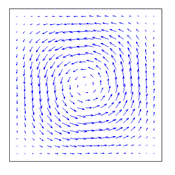
\includegraphics[height=4cm]{images/mms/Ex1_Q2Q1_velo.png}
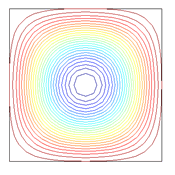
\includegraphics[height=4cm]{images/mms/Ex1_Q2Q1_streamlines.png}
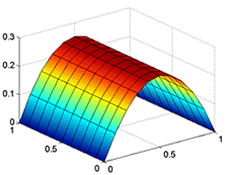
\includegraphics[height=4cm]{images/mms/Ex1_Q2Q1_pres.png}\\
{\small http://ww2.lacan.upc.edu/huerta/exercises/Incompressible/Incompressible\_Ex1.htm}
\end{center}

As shown in \cite{dohu03}, If the LBB condition is not satisfied, spurious oscillations spoil the pressure approximation. 
Figures below show results obtained with a mesh of 20x20 Q1P0 (left) and P1P1 (right) elements:
\begin{center}
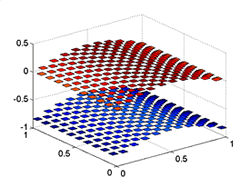
\includegraphics[height=5cm]{images/mms/Ex1_Q1P0_pres.png}
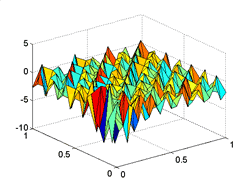
\includegraphics[height=5cm]{images/mms/Ex1_P1P1_pres.png}]]
{\small http://ww2.lacan.upc.edu/huerta/exercises/Incompressible/Incompressible\_Ex1.htm}
\end{center}

Taking into account that the proposed problem has got analytical solution, it is easy to analyze convergence of the different pairs of elements:
\begin{center}
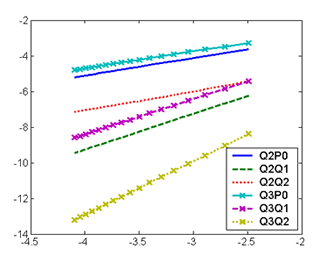
\includegraphics[height=7cm]{images/mms/Ex1_conv_qua.png}\\
{\small http://ww2.lacan.upc.edu/huerta/exercises/Incompressible/Incompressible\_Ex1.htm}
\end{center}

One can also compute the stress components:
\begin{eqnarray}
\sigma_{xx} &=&  2x^2(2x - 2)(4y^3 - 6y^2 + 2y) + 4x(-x + 1)^2*(4y^3 - 6y^2 + 2y) - x(-x + 1) + 1/6 \\
\sigma_{xy} &=&  x^2(-x + 1)^2*(12y^2 - 12y + 2) - y^2(-y + 1)^2*(12x^2 - 12x + 2) \\
\sigma_{yy} &=&  -x(-x + 1) - 2y^2(2y - 2)(4x^3 - 6x^2 + 2x) - 4y(-y + 1)^2(4x^3 - 6x^2 + 2x) + 1/6
\end{eqnarray}


All the necessary functions to do this benchmark are in {\tt mms/dh.py}:
\lstinputlisting[language=python]{mms/dh.py}


%-----------------------------------------------------------------------------
\subsubsection{Analytical benchmark II \label{mms2} - "DB2D"}

Taken from \cite{dobo04,bodg06}. It is for a unit square with $\nu=\mu/\rho=1$ and the smooth exact solution is
\begin{eqnarray}
u(x,y) &=& x+x^2 - 2xy+x^3 - 3xy^2 + x^2y \\
v(x,y) &=& -y-2xy+y^2 -3x^2y + y^3 - xy^2 \\
p(x,y) &=& xy+x+y+x^3y^2 - 4/3
\end{eqnarray}
Note that the pressure obeys $\int_{\Omega} p \; d\Omega = 0$

\begin{eqnarray}
b_x &=& - (1+y-3x^2y^2) \\
b_y &=& - (1-3x-2x^3y) 
\end{eqnarray}

This benchmark is also used in \cite{wosp14}.

%-----------------------------------------------------------------------------
\subsubsection{Analytical benchmark III \label{mms3} - "DB3D"}

This benchmark begins by postulating a polynomial solution 
to the 3D Stokes equation \cite{dobo04}:
\begin{equation}
{\bm v}
=
\left(
\begin{array}{c}
x+x^2+xy+x^3y \\
y + xy + y^2 + x^2 y^2\\
-2z - 3xz - 3yz - 5x^2 yz
\end{array}
\right)
\label{eqbur}
\end{equation}
and
\begin{equation}
p = xyz + x^3 y^3z - 5/32
\end{equation}
While it is then trivial to verify that this velocity field is divergence-free,  
the corresponding body force of the Stokes equation can be computed by  
inserting this solution into the momentum equation with a given viscosity $\mu$
(constant or position/velocity/strain rate dependent). 
The domain is a unit cube and velocity boundary conditions 
simply use Eq. (\ref{eqbur}). 
Note that the pressure fulfills 
\[
\int_\Omega p({\vec r}) d\Omega = 0.  
\]


\paragraph{Constant viscosity}
In this case, the right hand side writes:
\begin{eqnarray}
{\bm f} &=& 
-{\bm \nabla p} + 
\mu
\left(
\begin{array}{c}
2+6xy \\
2+2x^2+2y^2 \\
-10yz
\end{array}
\right) \nonumber\\
&=&
-
\left(
\begin{array}{c}
yz+3x^2 y^3z \\
xz+3 x^3 y^2 z \\
xy+x^3y^3
\end{array}
\right) 
+
\mu
\left(
\begin{array}{c}
2+6xy \\
2+2x^2+2y^2 \\
-10yz
\end{array}
\right)
\nonumber
\end{eqnarray}

We can compute the components of the strainrate tensor:
\begin{eqnarray}
\dot{\varepsilon}_{xx} &=& 1+2x+y+3x^2y\\
\dot{\varepsilon}_{yy} &=& 1+x+2y+2x^2y\\
\dot{\varepsilon}_{zz} &=& -2-3x-3y-5x^2y\\ 
\dot{\varepsilon}_{xy} &=&  \frac{1}{2} (x+y+2xy^2+x^3)\\
\dot{\varepsilon}_{xz} &=&  \frac{1}{2} (-3z-10xyz  )\\
\dot{\varepsilon}_{yz} &=&  \frac{1}{2} ( -3z -5x^2z )
\end{eqnarray}
Note that we of course have $\dot{\varepsilon}_{xx} +\dot{\varepsilon}_{yy} 
+\dot{\varepsilon}_{zz} =0$.

\paragraph{Variable viscosity}

In this case, the right hand side is obtained through
\begin{eqnarray}
{\bm f} &=& -{\bm \nabla p} + 
\mu
\left(
\begin{array}{c}
2+6xy \\
2+2x^2+2y^2 \\
-10yz
\end{array}
\right) \nonumber\\
&+&
\left(
\begin{array}{c}
2 \dot{\varepsilon}_{xx} \\
2 \dot{\varepsilon}_{xy} \\
2 \dot{\varepsilon}_{xz}
\end{array}
\right) \frac{\partial \mu}{\partial x}
+
\left(
\begin{array}{c}
2 \dot{\varepsilon}_{xy} \\
2 \dot{\varepsilon}_{yy} \\
2 \dot{\varepsilon}_{yz}
\end{array}
\right) \frac{\partial \mu}{\partial y}
+
\left(
\begin{array}{c}
2 \dot{\varepsilon}_{xz} \\
2 \dot{\varepsilon}_{yz} \\
2 \dot{\varepsilon}_{zz} 
\end{array}
\right) \frac{\partial \mu}{\partial z}
\end{eqnarray}


The viscosity can be chosen to be a smooth varying function:
\begin{equation}
\mu = exp(1 - \beta(x(1 - x) + y(1 - y) + z(1 - z)))
\end{equation}
Choosing $\beta=0$ yields a constant velocity $\mu=e^1$ (and greatly simplifies the right-hand side).
One can easily show that the ratio of viscosities $\mu^\star$
in the system follows $\mu^\star=\exp(-3\beta/4)$ so that choosing $\beta=10$ yields
$\mu^\star\simeq 1808$ and $\beta=20$ yields $\mu^\star\simeq 3.269\times10^6$.
In this case
\begin{eqnarray}
\frac{\partial \mu}{\partial x}&=&-4\beta(1-2x)\mu(x,y,z)\\
\frac{\partial \mu}{\partial y}&=&-4\beta(1-2y)\mu(x,y,z)\\
\frac{\partial \mu}{\partial z}&=&-4\beta(1-2z)\mu(x,y,z)
\end{eqnarray}


\cite{busa13} has carried out this benchmark for $\beta=4$, i.e.: 
\[
\mu(x,y,z)=\exp ( 1-4( x(1-x)+y(1-y)+z(1-z)  )  )
\]
In a unit cube, this yields a variable viscosity such that
$0.1353 < \mu <   2.7182$, i.e. a ratio of approx. 20 within the domain. We then have:
\begin{eqnarray}
\frac{\partial \mu}{\partial x}&=&-4(1-2x)\mu(x,y,z)\\
\frac{\partial \mu}{\partial y}&=&-4(1-2y)\mu(x,y,z)\\
\frac{\partial \mu}{\partial z}&=&-4(1-2z)\mu(x,y,z)
\end{eqnarray}

\todo[inline]{sort out mess wrt Eq 26 of busa13}


%-----------------------------------------------------------------------------
\subsubsection{Analytical benchmark IV \label{mms4} - "Bercovier \& Engelman"}

From \cite{been79}. The two-dimensional domain is a unit square. The body forces are:
\begin{eqnarray}
f_x &=& 128[ x^2(x-1)^2 12 (2y-1) + 2 (y-1)(2y-1)y(12x^2-12x+2)  ] \nn\\
f_y &=& 128[ y^2(y-1)^2 12 (2x-1) + 2 (x-1)(2x-1)y(12y^2-12y+2)  ] \nn\\
\end{eqnarray}
The solution is
\begin{eqnarray}
u &=& -256x^2(x-1)^2y(y-1)(2y-1) \nn\\
v &=&  256x^2(y-1)^2x(x-1)(2x-1) \nn\\
p &=& 0 
%p &=& (x-1/2)(y-1/2) 
\end{eqnarray}

Another choice:
\begin{eqnarray}
f_x &=& 128[ x^2(x-1)^2 12 (2y-1) + 2 (y-1)(2y-1)y(12x^2-12x+2)  ] + y - 1/2 \nn\\
f_y &=& 128[ y^2(y-1)^2 12 (2x-1) + 2 (x-1)(2x-1)y(12y^2-12y+2)  ] + x - 1/2 \nn\\
\end{eqnarray}
The solution is
\begin{eqnarray}
u &=& -256x^2(x-1)^2y(y-1)(2y-1) \nn\\
v &=&  256x^2(y-1)^2x(x-1)(2x-1) \nn\\
p &=& (x-1/2)(y-1/2) 
\end{eqnarray}


%-----------------------------------------------------------------------------
\subsubsection{Analytical benchmark V \label{mms5} - "VJ1"}

This is taken from Appendix D1 of \cite{john16}.

The domain $\Omega$ is a unit square. We consider the stream function
\[
\phi(x,y)=1000x^2(1-x)^4y^3(1-y)^2
\]
The velocity field is defined by
\begin{eqnarray}
u(x,y) &=&  \partial_y \phi = 1000(x^2(1-x)^4 y^2 (1-y)(3-5y)  ) \\
v(x,y) &=& -\partial_x \phi = 1000(-2x(1-x)^3(1-3x)y^3(1-y)^2)
\end{eqnarray}
and it is easy to verify that $\vec\nabla\cdot\vec v=0$.

The pressure is given by:
\[
p(x,y)=\pi^2( xy^3\cos(2\pi x^2y) - x^2y \sin(2\pi xy)) + \frac{1}{8}
\]

\begin{center}
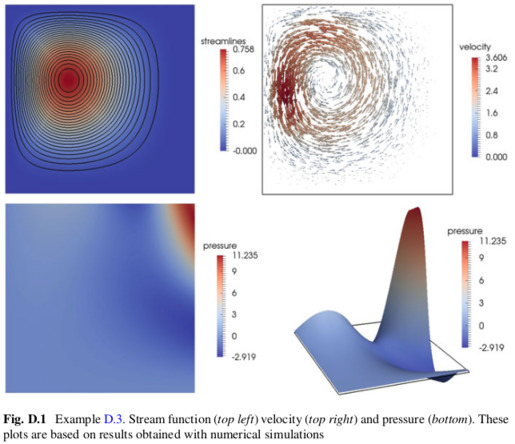
\includegraphics[width=8cm]{images/mms/mms5}\\
Taken from \cite{john16}.
\end{center}

\bscthesis \index{BSc Thesis}

%-----------------------------------------------------------------------------
\subsubsection{Analytical benchmark VI \label{mms6} - "Ilinca \& Pelletier"}
\index{Poiseuille flow} \index{Shear Heating}

This is taken from \cite{ilpe07}.

Let us consider the Poiseuille flow of a Newtonian fluid. The channel has 
isothermal flat walls located at $y=\pm h$. The velocity distribution is parabolic:
\[
u = u_0 \left(1-\frac{y^2}{h^2} \right) 
\quad\quad\quad
v=0
\]
where $u_0$ is the maximum velocity. The (steady state) temperature field is the solution of
the advection-diffusion equation:
\[
\rho C_p \vec v \cdot \vec\nabla T
= k \Delta T + \Phi
\]
where $\Phi$ is the dissipation function given by
\[
\Phi
=\eta \left[  
2\left(\frac{\partial u}{\partial x} \right)^2 + 
2\left(\frac{\partial v}{\partial y} \right)^2 +
\left( \frac{\partial v}{\partial x} + \frac{\partial u}{\partial y} \right)^2
\right]
=
\eta \left( \frac{\partial u}{\partial y} \right)^2 = 4 \eta \frac{u_0^2 y^2}{h^4}
\]
We logically assume that $T=T(y)$ so that $\partial T/\partial x=0$ and $\vec v \cdot \vec\nabla T=0$.
We then have to solve:
\[
k \frac{\partial^2 T}{\partial y^2} + 4 \eta \frac{u_0^2 y^2}{h^4} = 0
\]
We can integrate twice and use the boundary conditions $T(y=\pm h)=T_0$ to arrive at:
\[
T(y) = T_0 + \frac{1}{3} \frac{\eta u_0^2}{k} \left[ 1-\left(\frac{y}{h}\right)^4  \right]
\]
with a maximum temperature
\[
T_M = T(y=0) = T_0 + \frac{1}{3} \frac{\eta u_0^2}{k} 
\]

%-----------------------------------------------------------------------------
\subsubsection{Analytical benchmark VII \label{mms7} - "grooves"}

This benchmark was designed by Dave May. 
The velocity and pressure fields are given by
\begin{eqnarray}
u(x,y) &=& x^3 y + x^2 + xy + x \nn\\
v(x,y) &=& -\frac{3}{2}x^2y^2 - 2xy - \frac{1}{2}y^2 - y \nn\\
p(x,y) &=& x^2y^2 + xy + 5 + p_0
\end{eqnarray}
where $p_0$ is a constant to be determined based on the type of pressure normalisation.
The viscosity is chosen to be
\begin{equation}
\eta(x,y)=-\sin(p)+1+\epsilon = -\sin (x^2y^2 + xy + 5) + 1 + \epsilon 
\end{equation}
where $\epsilon$ actually controls the viscosity contrast. Note that inserting the polynomial 
expression of the pressure inside the viscosity expression makes the problem linear. 
We have
\begin{eqnarray}
\dot{\varepsilon}_{xx} = \frac{\partial u}{\partial x} &=& 3x^2y+2x+y+1 \nn\\
\dot{\varepsilon}_{yy} = \frac{\partial v}{\partial y} &=& -3x^2y-2x-y-1 \nn\\
\dot{\varepsilon}_{xy} = \frac{1}{2}\left(\frac{\partial u}{\partial y} + \frac{\partial v}{\partial x} \right)
&=& \frac{1}{2}\left(x^3+x-3xy^2-2y \right)
\end{eqnarray}
and we can verify that the velocity field is incompressible since ${\vec \nabla}\cdot{\vec \upnu} = 
\dot{\varepsilon}_{xx} + \dot{\varepsilon}_{yy} =0$.
The pressure gradient is given by
\begin{eqnarray}
\frac{\partial p}{\partial x} &=& 2xy^2+y \nn\\
\frac{\partial p}{\partial y} &=& 2x^2y+x \nn
\end{eqnarray}
The right hand side term of the Stokes equation is such that
\begin{eqnarray}
 - \frac{\partial p}{\partial x} + \frac{\partial s_{xx}}{\partial x} + \frac{\partial s_{yx}}{\partial y} +f_x&=&0\nn\\
 - \frac{\partial p}{\partial y} + \frac{\partial s_{xy}}{\partial x} + \frac{\partial s_{yy}}{\partial y} +f_y&=&0
\end{eqnarray}
with 
\begin{eqnarray}
\frac{\partial s_{xx}}{\partial x} 
&=& \frac{\partial (2 \eta \dot{\varepsilon}_{xx}) }{\partial x} = 2 \eta \frac{\partial  \dot{\varepsilon}_{xx} }{\partial x} +  2\frac{\partial \eta }{\partial x} \dot{\varepsilon}_{xx} \nn\\
\frac{\partial s_{zx}}{\partial z} 
&=& \frac{\partial (2 \eta \dot{\varepsilon}_{zx}) }{\partial z} = 2 \eta \frac{\partial  \dot{\varepsilon}_{zx} }{\partial z} +  2\frac{\partial \eta }{\partial z} \dot{\varepsilon}_{zx} \nn\\
\frac{\partial s_{xz}}{\partial x} 
&=& \frac{\partial (2 \eta \dot{\varepsilon}_{xz}) }{\partial x} = 2 \eta \frac{\partial  \dot{\varepsilon}_{xz} }{\partial x} +  2\frac{\partial \eta }{\partial x} \dot{\varepsilon}_{xz} \nn\\
\frac{\partial s_{zz}}{\partial z} 
&=& \frac{\partial (2 \eta \dot{\varepsilon}_{zz}) }{\partial z} = 2 \eta \frac{\partial  \dot{\varepsilon}_{zz} }{\partial z} +  2\frac{\partial \eta }{\partial z} \dot{\varepsilon}_{zz} \nn\\
\frac{\partial \eta }{\partial x} &=& -z (2 x z + 1) \cos(x^2 z^2 + x z + 5) \nn\\
\frac{\partial \eta }{\partial z} &=& -x (2 x z + 1) \cos(x^2 z^2 + x z + 5) \nn\\
\frac{\partial  \dot{\varepsilon}_{xx} }{\partial x} &=& 6xz+2 \nn\\
\frac{\partial  \dot{\varepsilon}_{zx} }{\partial z} &=& -3xz-1  \nn\\
\frac{\partial  \dot{\varepsilon}_{xz} }{\partial x} &=& \frac{1}{2}(3x^2+1-3z^2)  \nn\\
\frac{\partial  \dot{\varepsilon}_{zz} }{\partial z} &=& -3x^2-1  \nn
\end{eqnarray}

\index{pressure nullspace}
Velocity boundary conditions are prescribed on all four boundaries so that the pressure is known up to a constant
(the pressure solution has a nullspace), 
and the $p_0$ constant can be determined by requiring that
\[
\int_0^L\int_0^L p(x,y) \; dx dy = 
\int_0^L\int_0^L (x^2y^2+xy+5) dx dy + \int_0^L \int_0^L p_0 \; dxdy = 
\int_0^L\int_0^L (x^2y^2+xy+5) dx dy + p_0 L^2 =0 
\]
where $L$ is the size of the square domain.
Then
\[
p_0 =-  \frac{1}{L^2}  \int_0^L\int_0^L (x^2y^2+xy+5) dx dy
= -\frac{L^4}{9}-\frac{L^2}{4} - 5 
\]
\[
\]
%\begin{itemize}
%\item
%When the domain is $1\times 1$, $p_0=-\frac{1}{9}-\frac{1}{4} - 5 = -193/36$.
%\item
%When the domain is $2\times 2$, $p_0=-\frac{16}{9}-\frac{4}{4} - 5*4 = -70/9$.
%\item
%When the domain is $3\times 3$, $p_0=-\frac{81}{9}-\frac{9}{4} - 5*9 = -585/16$.
%\item
%When the domain is $4\times 4$, $p_0=-\frac{256}{9}-\frac{16}{4} - 5*16 = -1348/9$.
%\end{itemize}

As seen in the following figure, the value of $\epsilon$ controls the viscosity field amplitude.
This is simply explained by the fact that when the $\sin$ term of the viscosity takes value 1, the viscosity
is then equal to $\epsilon$.
\begin{center}
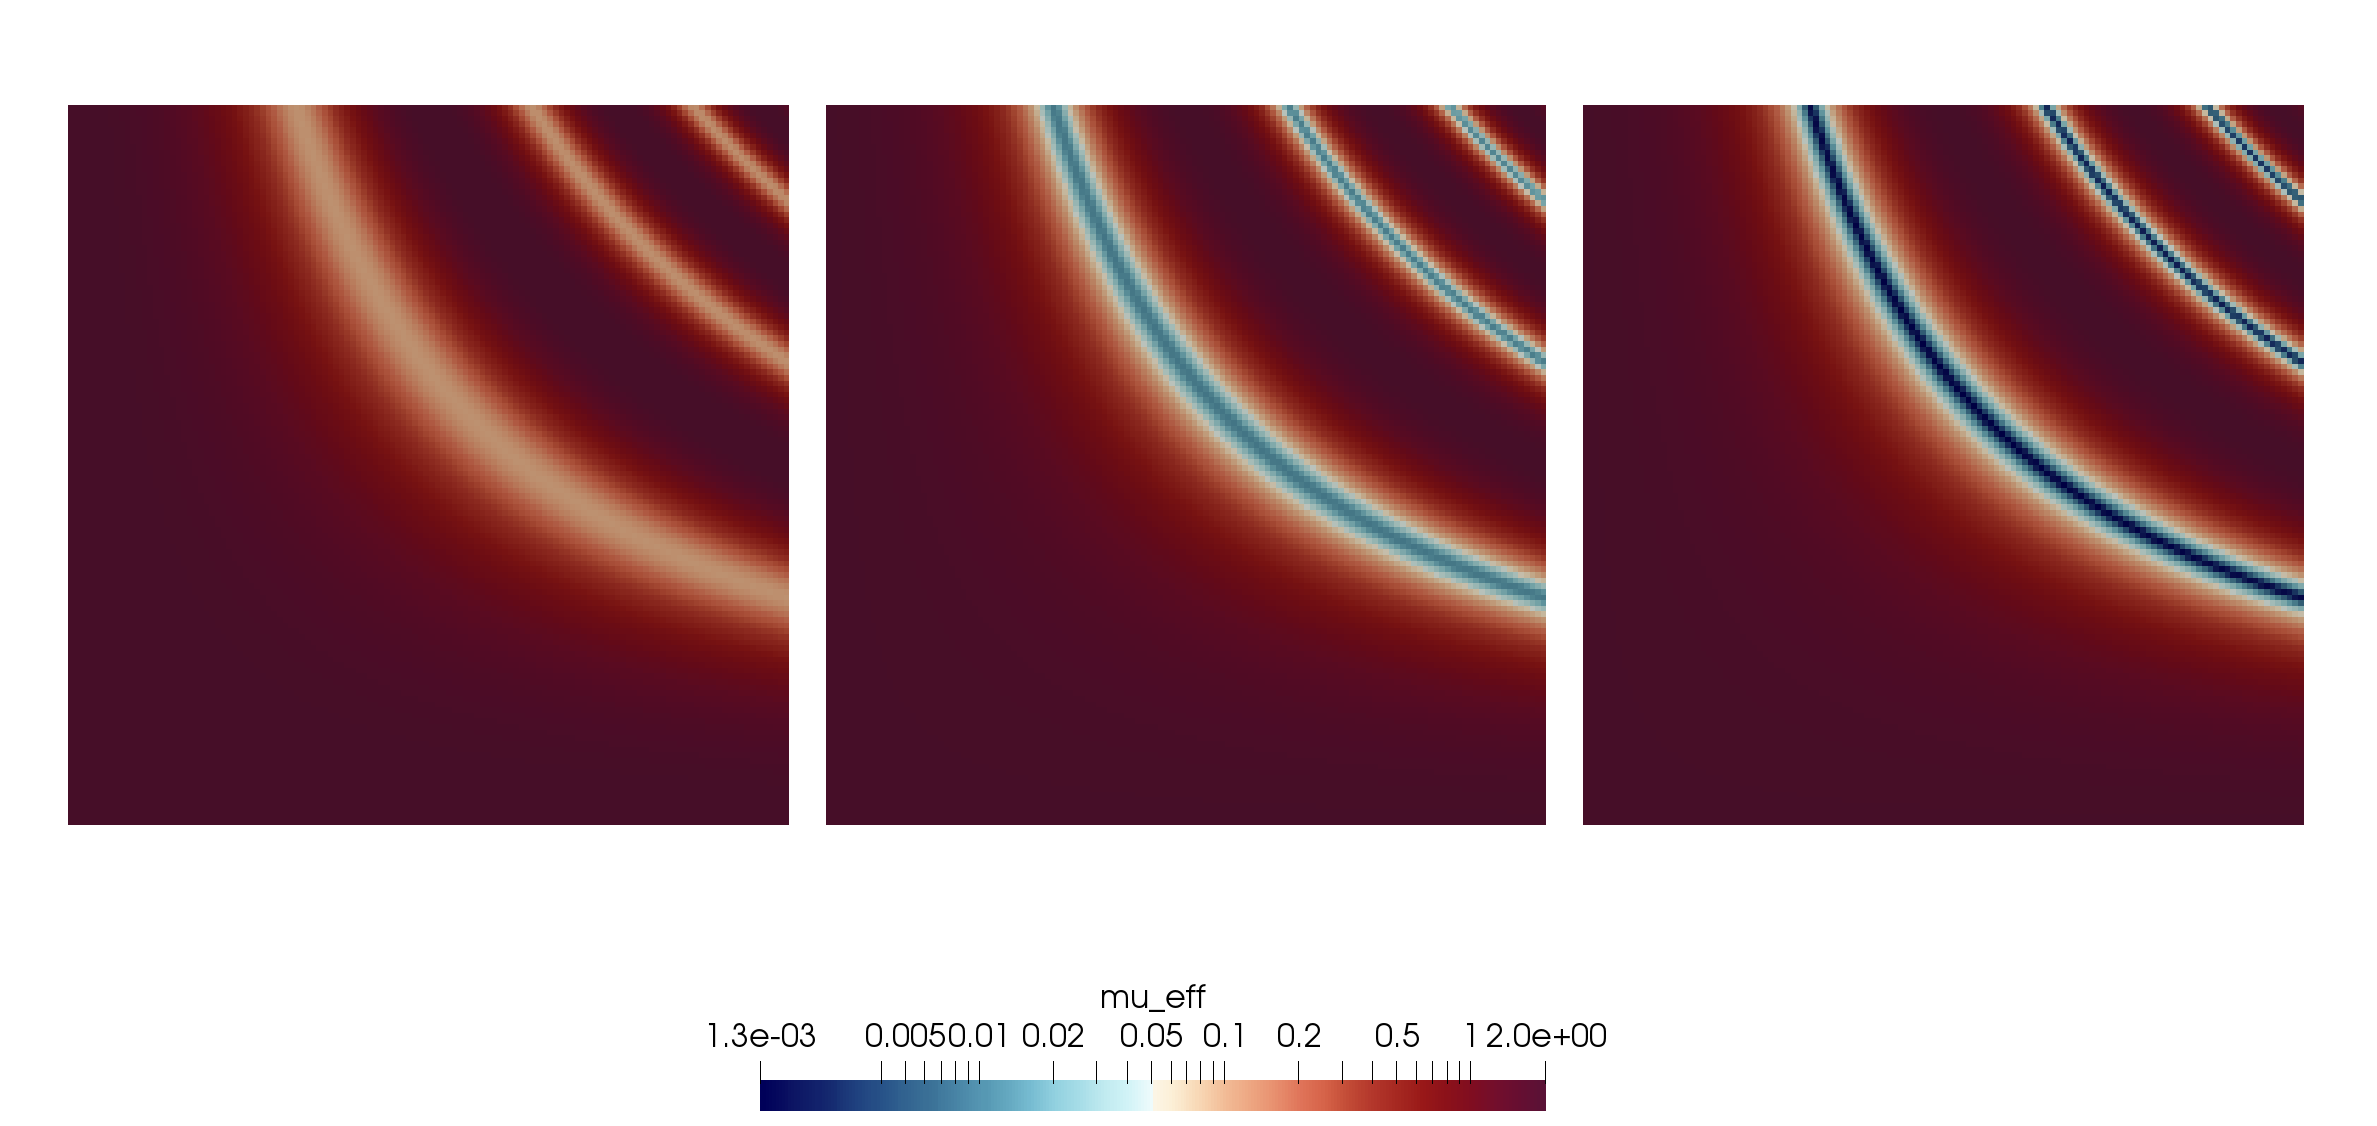
\includegraphics[width=14cm]{images/mms/mms7_mueffs}\\
Domain size 2x2 with $\epsilon=0.1, 0.01, 0.001$
\end{center}

Another interesting aspect of this benchmark is the fact that increasing the domain size
adds complexity to it as it increases the number of low viscosity zones and the spacing 
between them also decreases:

\begin{center}
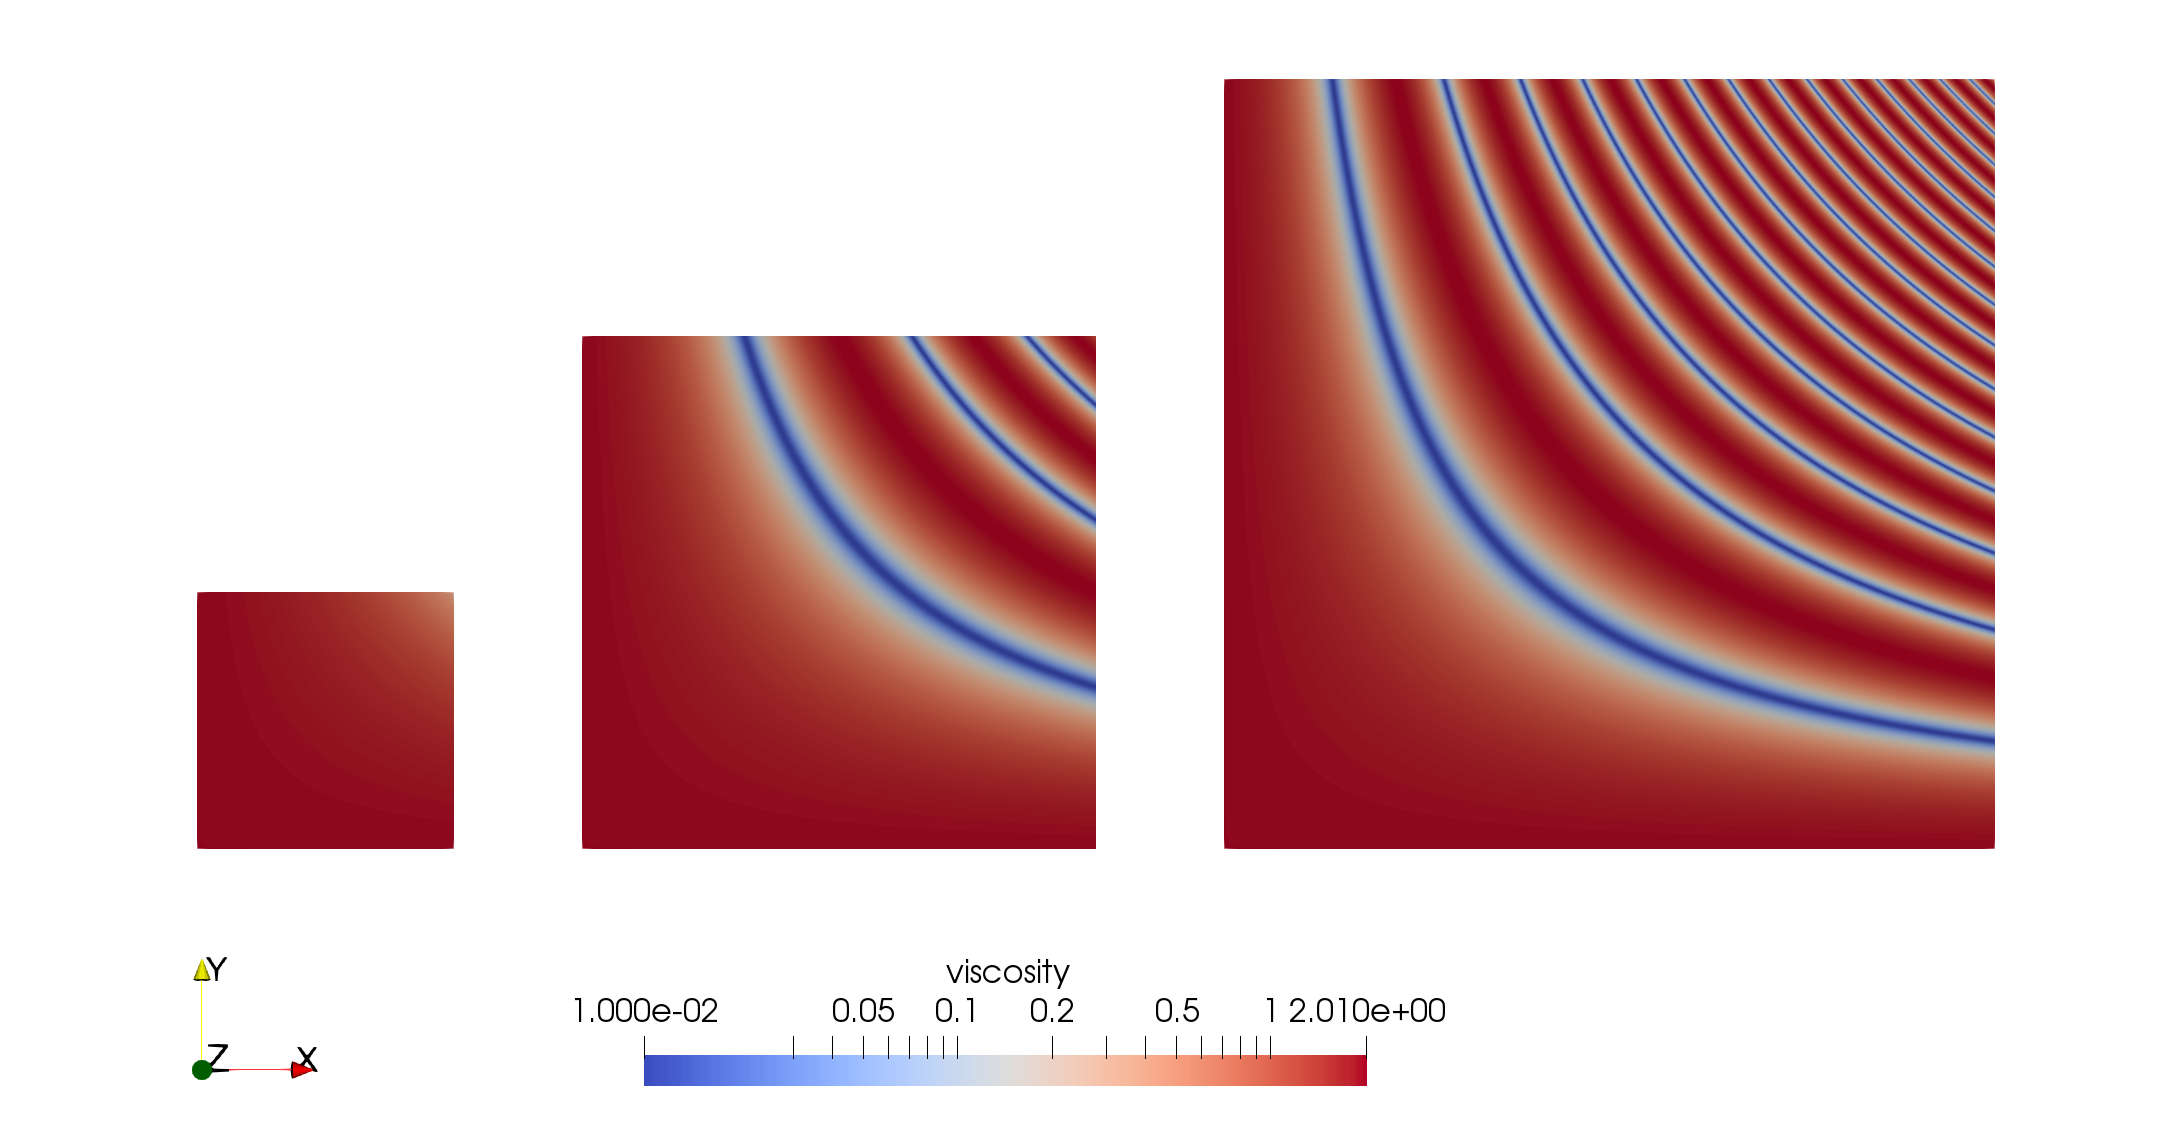
\includegraphics[width=7.28cm]{images/mms/mms7_visc}
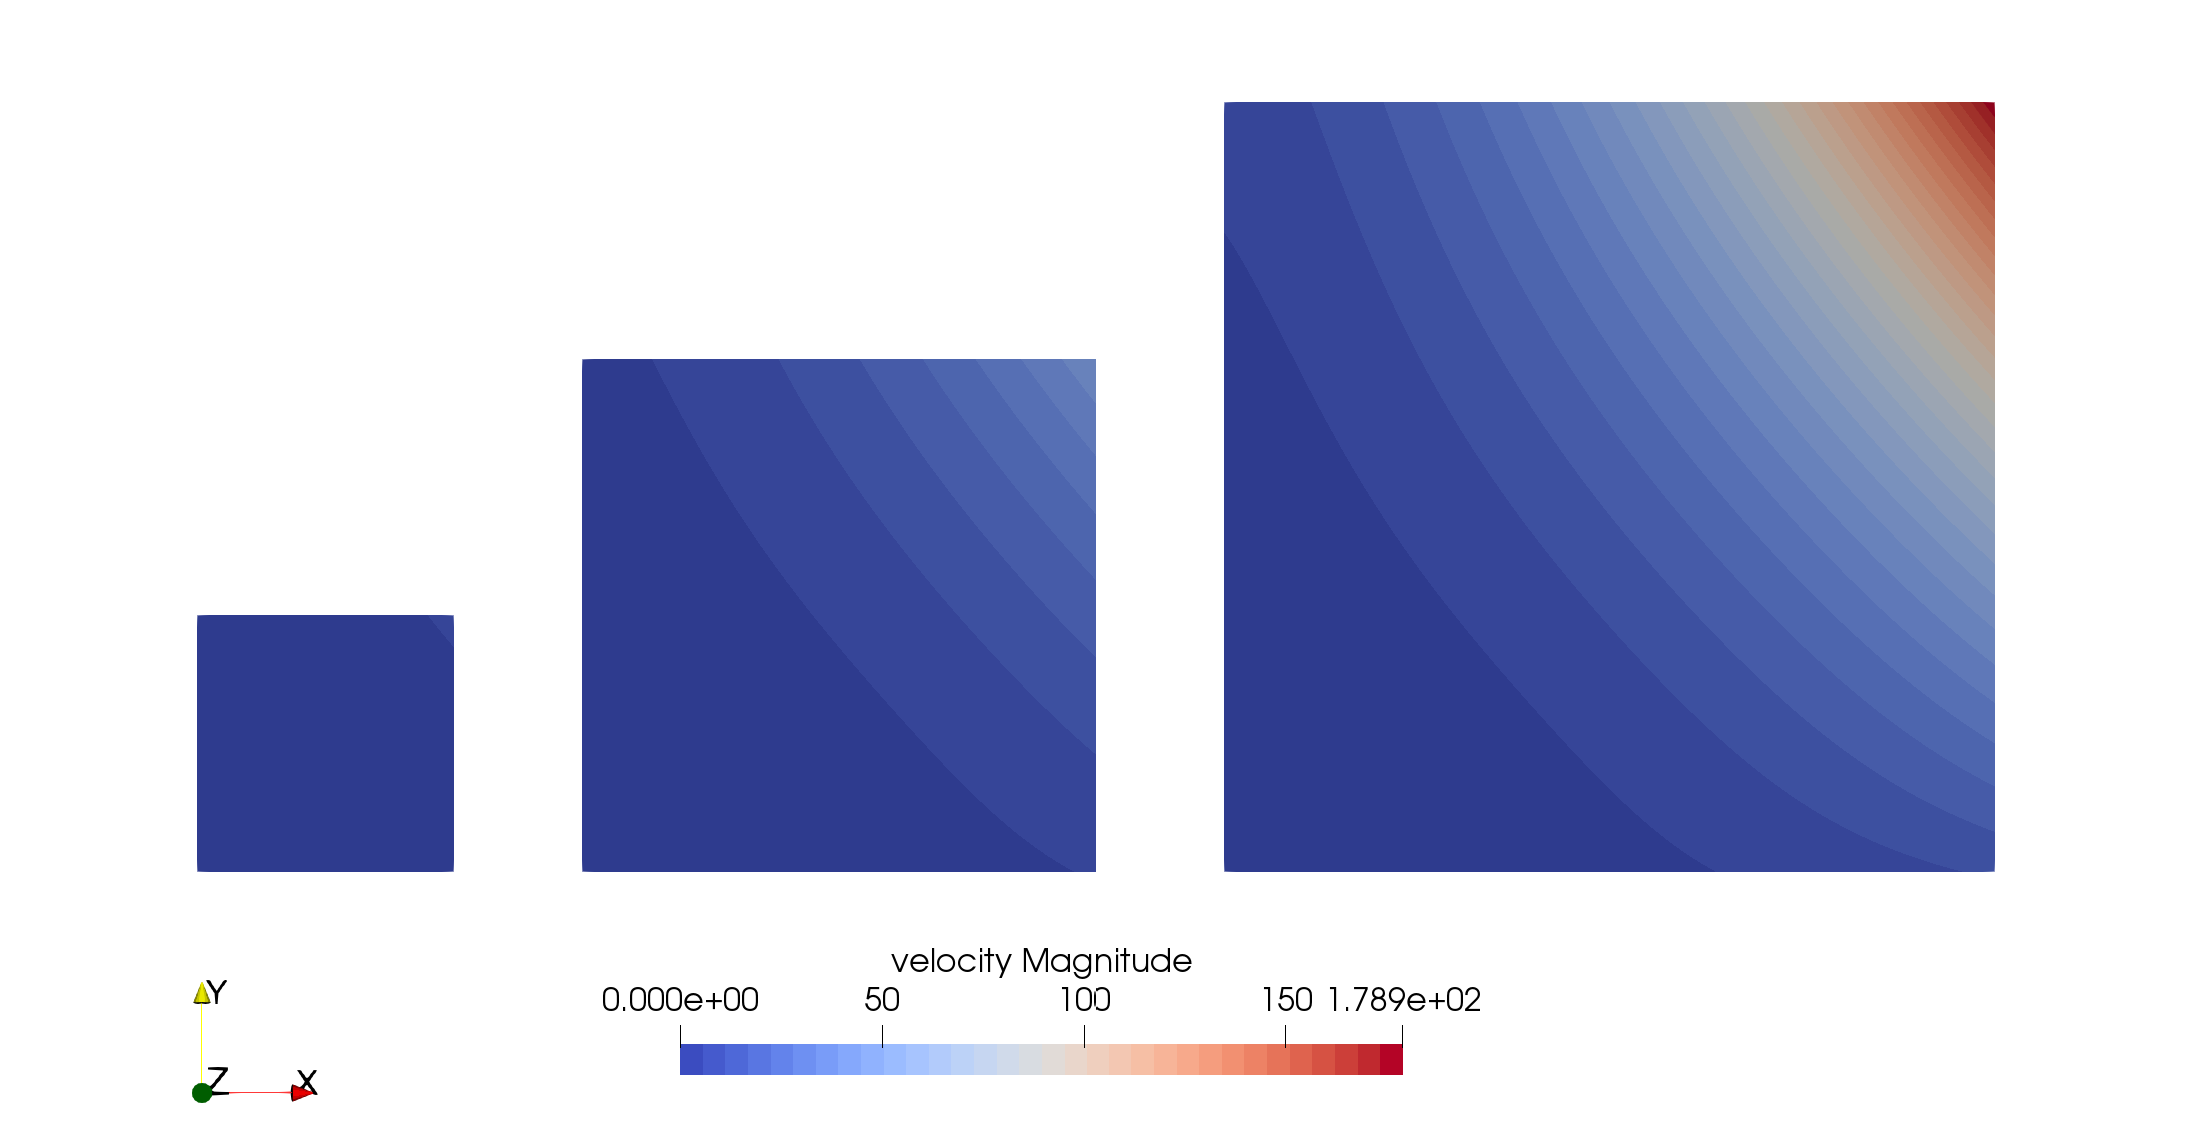
\includegraphics[width=7.28cm]{images/mms/mms7_vel}\\
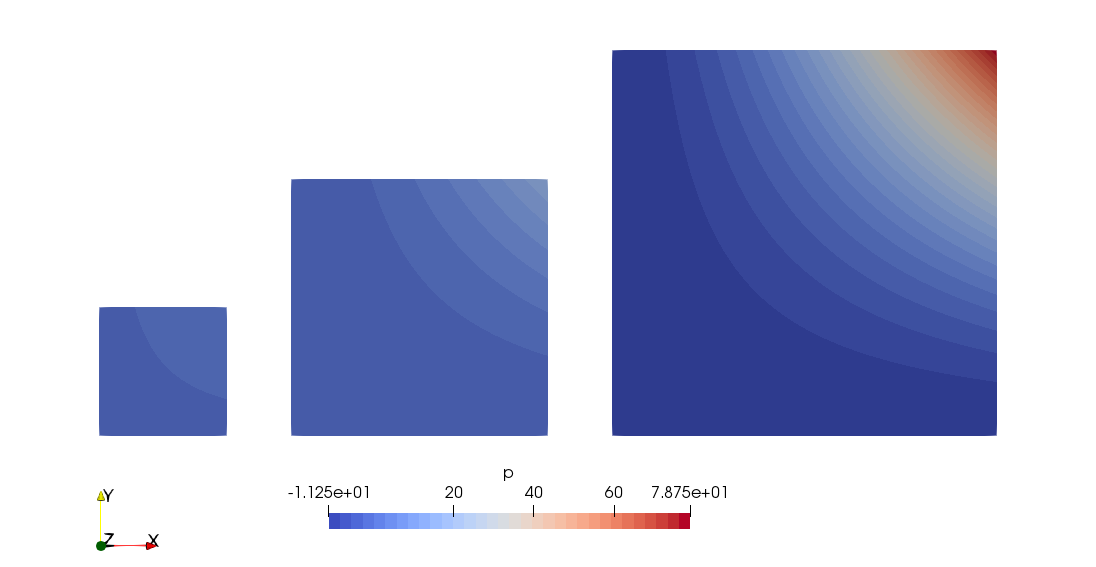
\includegraphics[width=7.28cm]{images/mms/mms7_press}
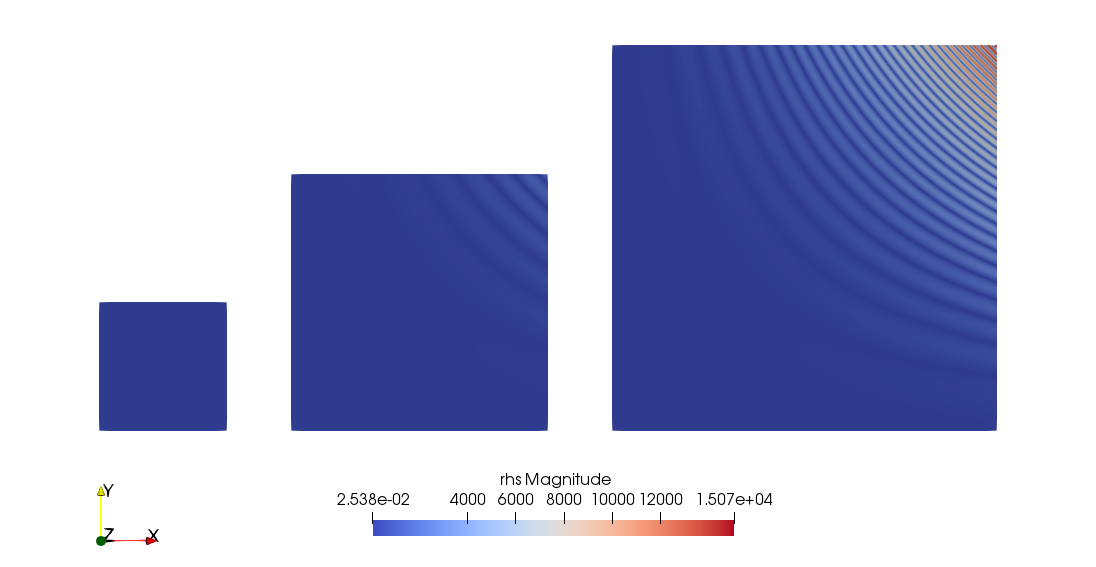
\includegraphics[width=7.28cm]{images/mms/mms7_rhs}\\
Three different domain sizes (1x1, 2x2, 3x3) with $\epsilon=0.001$.
\end{center}


Finally, because the analytical expression for both components of the velocity is a polynomial, we can also
compute the root mean square velocity exactly. For instance, for a 2x2 domain:
\begin{center}
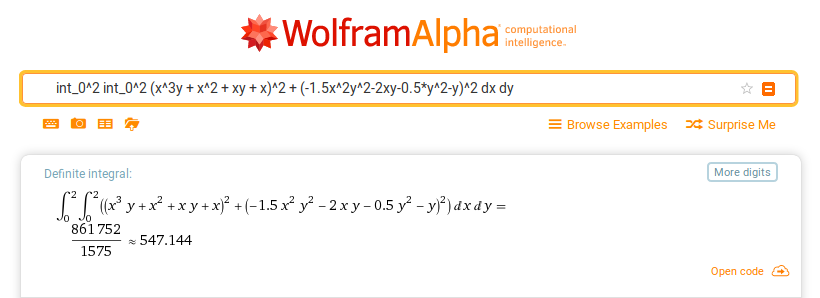
\includegraphics[width=8cm]{images/mms/mms7_vrmstheo}
\end{center}
and we end up with (for $L=2$)
\[
v_{rms} = \sqrt{\frac{1}{L^2}\frac{861752}{1575}} = \sqrt{\frac{215438}{1575}}
\simeq 11.6955560683
\]

\bscthesis \index{BSc Thesis}

%-----------------------------------------------------------------------------
\subsubsection{Analytical benchmark VIII \label{mms8} - "Kovasznay"}

This flow was published by L.I.G. Kovasznay in 1948 \cite{kova48}. 
This paper presents an exact two-dimensional solution of the Navier-Stokes equations 
with a periodicity in the vertical direction, 
gives an analytical solution to the steady-state Navier-Stokes equations that is similar
which is a flow-field behind a periodic array of cylinders.

\[
u(x,y)=1-\exp(\lambda x) \cos (2\pi y)
\qquad
\qquad
v(x,y)=\frac{\lambda}{2\pi} \exp(\lambda x) \sin (2 \pi y)
\qquad
\qquad
\lambda=\frac{Re}{2}-\sqrt{\frac{Re^2}{4}+4\pi^2}
\]

Following step-55 of deal.II \footnote{\url{https://www.dealii.org/current/doxygen/deal.II/step_55.html}}
we have to 'cheat' here since we are not solving the non-linear Navier-Stokes equations, but the linear Stokes system without convective term. Therefore, to recreate the exact same solution
we move the convective term into the right-hand side.

The analytical solution is prescribed left and right, while free/no (??) slip is prescribed at top and bottom.

Solution as implemented in step-55:
\begin{verbatim}
const double pi2 = pi*pi;
  u = -exp(x*(-sqrt(25.0 + 4*pi2) + 5.0))*cos(2*y*pi) + 1;
  v = (1.0L/2.0L)*(-sqrt(25.0 + 4*pi2) + 5.0)*exp(x*(-sqrt(25.0 + 4*pi2) + 5.0))*sin(2*y*pi)/pi;
  p = -1.0L/2.0L*exp(x*(-2*sqrt(25.0 + 4*pi2) + 10.0)) 
- 2.0*(-6538034.74494422 + 0.0134758939981709*exp(4*sqrt(25.0 + 4*pi2)))/(-80.0*exp(3*sqrt(25.0 + 4*pi2)) 
+ 16.0*sqrt(25.0 + 4*pi2)*exp(3*sqrt(25.0 + 4*pi2))) 
- 1634508.68623606*exp(-3.0*sqrt(25.0 + 4*pi2))/(-10.0 + 2.0*sqrt(25.0 + 4*pi2)) 
+ (-0.00673794699908547*exp(sqrt(25.0 + 4*pi2)) 
+ 3269017.37247211*exp(-3*sqrt(25.0 + 4*pi2)))/(-8*sqrt(25.0 + 4*pi2) + 40.0) 
+ 0.00336897349954273*exp(1.0*sqrt(25.0 + 4*pi2))/(-10.0 + 2.0*sqrt(25.0 + 4*pi2));
\end{verbatim}


%-----------------------------------------------------------------------------
\subsubsection{Analytical benchmark IX \label{mms9} - "VJ2"}

It is presented in \cite{jolm17} and meant to be a peculiar case where the velocity solution 
is exactly zero. The viscosity is 1, the domain is a unit square, no-slip boundary conditions 
are prescribed everywhere. The buoyancy force is given by $\vec{b}=(0,Ra(1-y+3y^2))$ where 
$Ra>0$ is a parameter. The flow is incompressible and the analytical pressure solution 
is given by $p=Ra(y^3-y^2/2+y-7/12)$.

%-----------------------------------------------------------------------------
\subsubsection{Analytical benchmark X \label{mms10} - "VJ3"}

This benchmark comes from John et al. \cite{jolm17}.
The domain is once again the unit square. The velocity field has the form of a large vortex.

\begin{eqnarray}
u(x,y) &=& 200x^2(1-x)^2y(1-y)(1-2y) \\
v(x,y) &=& -200x(1-x)(1-2x)y^2(1-y)^2 \\
p(x,y) &=& 10\left[(x-1/2)^3y^2+(1-x)^3(y-1/2)^3 \right]
\end{eqnarray}

\begin{center}
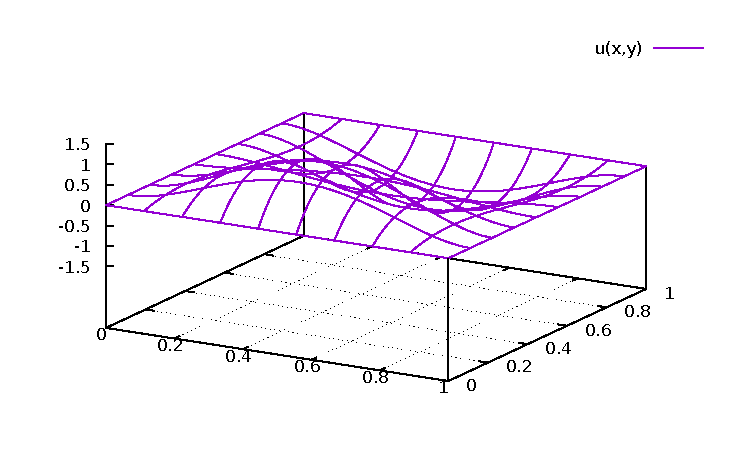
\includegraphics[width=4.5cm]{images/benchmark_VJ3/u.pdf}
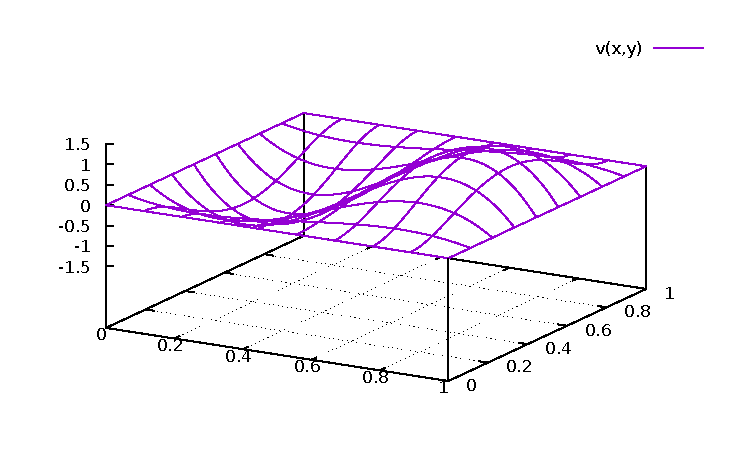
\includegraphics[width=4.5cm]{images/benchmark_VJ3/v.pdf}
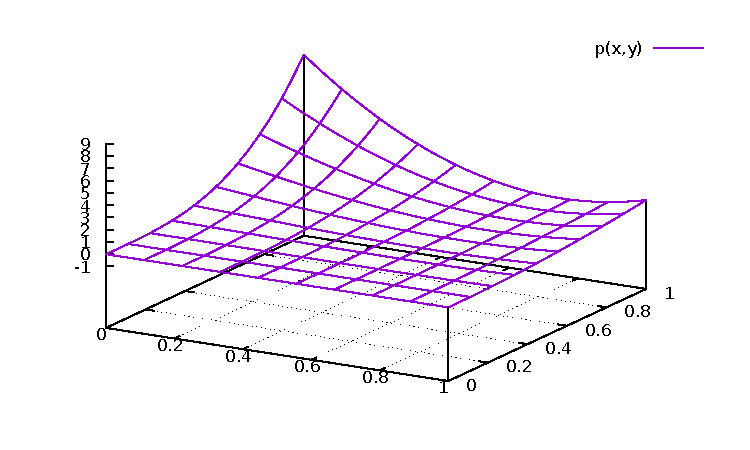
\includegraphics[width=4.5cm]{images/benchmark_VJ3/p.pdf}
\end{center}

\begin{eqnarray}
\dot{\varepsilon}_{xx}=\frac{\partial u}{\partial x} &=& -400(1-x)x(2x-1)(y-1)y(2y-1)  \\
\frac{\partial u}{\partial y} &=& 200(1-x)^2x^2 (6y^2-6y+1)  \\
\frac{\partial v}{\partial x} &=& -200(6x^2-6x+1)(1-y)^2y^2  \\
\dot{\varepsilon}_{yy}=\frac{\partial v}{\partial y} &=& 400(x-1)x(2x-1)(1-y)y(2y-1) 
\end{eqnarray}
so that 
\begin{eqnarray}
\dot{\varepsilon}_{xy}
&=&\frac{1}{2} \left[ 200(1-x)^2x^2 (6y^2-6y+1)   -200(6x^2-6x+1)(1-y)^2y^2  \right] \nn\\
&=&100(1-x)^2x^2 (6y^2-6y+1)   -100(6x^2-6x+1)(1-y)^2y^2 
\end{eqnarray}
Also
\begin{eqnarray}
\frac{\partial \dot{\varepsilon}_{xx}}{\partial x} &=& 400(6x^2-6x+1)y(2y^2-3y+1) \nn\\
\frac{\partial \dot{\varepsilon}_{xy}}{\partial x} 
&=& 200 (-2 x^2 (1 - x) (6 y^2 - 6 y + 1) + 2 x (1 - x)^2 (6 y^2 - 6 y + 1) - 6 (2 x - 1) (1 - y)^2 y^2)\nn\\
&=&  100 (-2 x^2 (1 - x) (6 y^2 - 6 y + 1) + 2 x (1 - x)^2 (6 y^2 - 6 y + 1) - 6 (2 x - 1) (1 - y)^2 y^2) \nn\\
\frac{\partial \dot{\varepsilon}_{xy}}{\partial y} &=& 400 (6 x^2 - 6 x + 1) (1 - y) y^2 + 200 (1 - x)^2 x^2 (12 y - 6) - 400 (6 x^2 - 6 x + 1) (1 - y)^2 y   \nn \\
\frac{\partial \dot{\varepsilon}_{yy}}{\partial y} &=& -400x(2x^2-3x+1)(6y^2-6y+1) 
\end{eqnarray}


\begin{eqnarray}
\frac{\partial p}{\partial x} &=& 30(x-1/2)^2y^2-30(1-x)^2(y-1/2)^3 \\
\frac{\partial p}{\partial y} &=& 20(x-1/2)^3y + 30(1-x)^3(y-1/2)^2  
\end{eqnarray}

From $\vec\nabla\cdot{\bm \sigma}+\vec{b}=\vec{0}$ we can obtain the rhs as follows:
\begin{eqnarray}
\vec{b} 
&=& - \vec\nabla\cdot{\bm \sigma} \nn\\ 
&=& \vec\nabla p -  \vec\nabla\cdot{\bm s} \nn\\ 
&=& \vec\nabla p -  \vec\nabla\cdot(2 \eta \dot{\bm \varepsilon})  
\end{eqnarray}
Assuming $\eta=1$ we arrive at:
\begin{eqnarray}
b_x &=&  \frac{\partial p}{\partial x} 
-2\frac{\partial \dot{\varepsilon}_{xx}}{\partial x}  
-2\frac{\partial \dot{\varepsilon}_{xy}}{\partial y}  \\
b_y &=&  \frac{\partial p}{\partial y}  
-2\frac{\partial \dot{\varepsilon}_{xy}}{\partial x} 
-2\frac{\partial \dot{\varepsilon}_{yy}}{\partial y}  
\end{eqnarray}

All the necessary functions to do this benchmark are in {\tt mms/vj3.py}:
\lstinputlisting[language=python]{mms/vj3.py}

\begin{center}
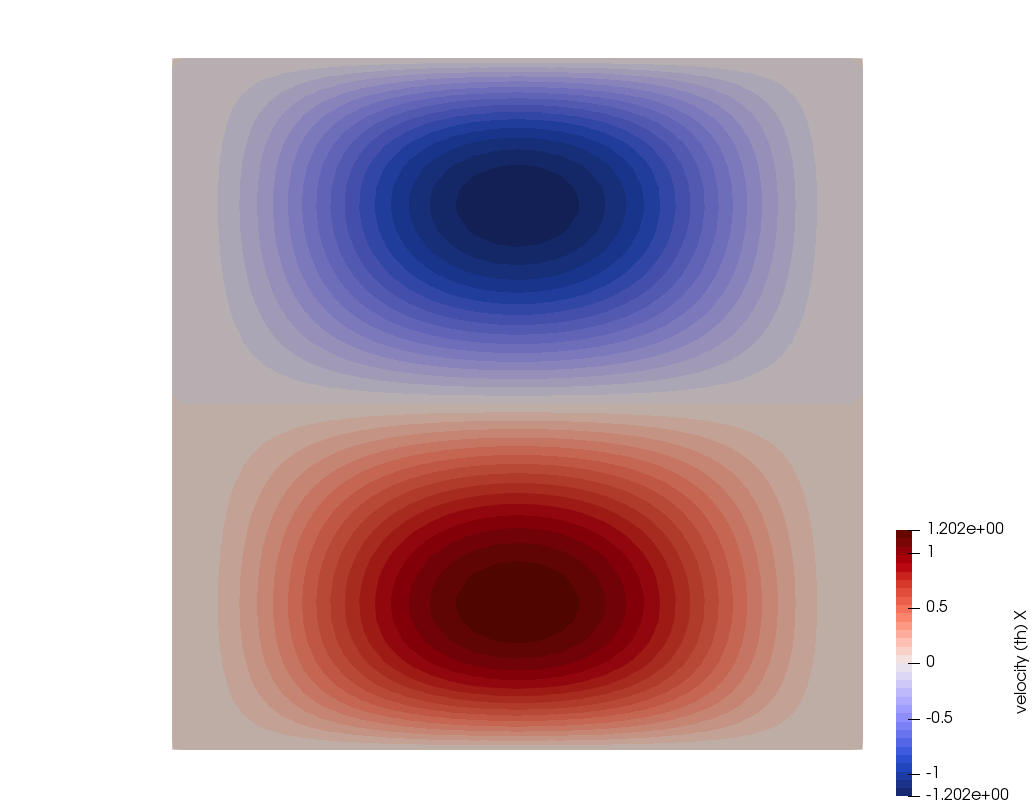
\includegraphics[width=4.5cm]{images/mms/vj3/u}
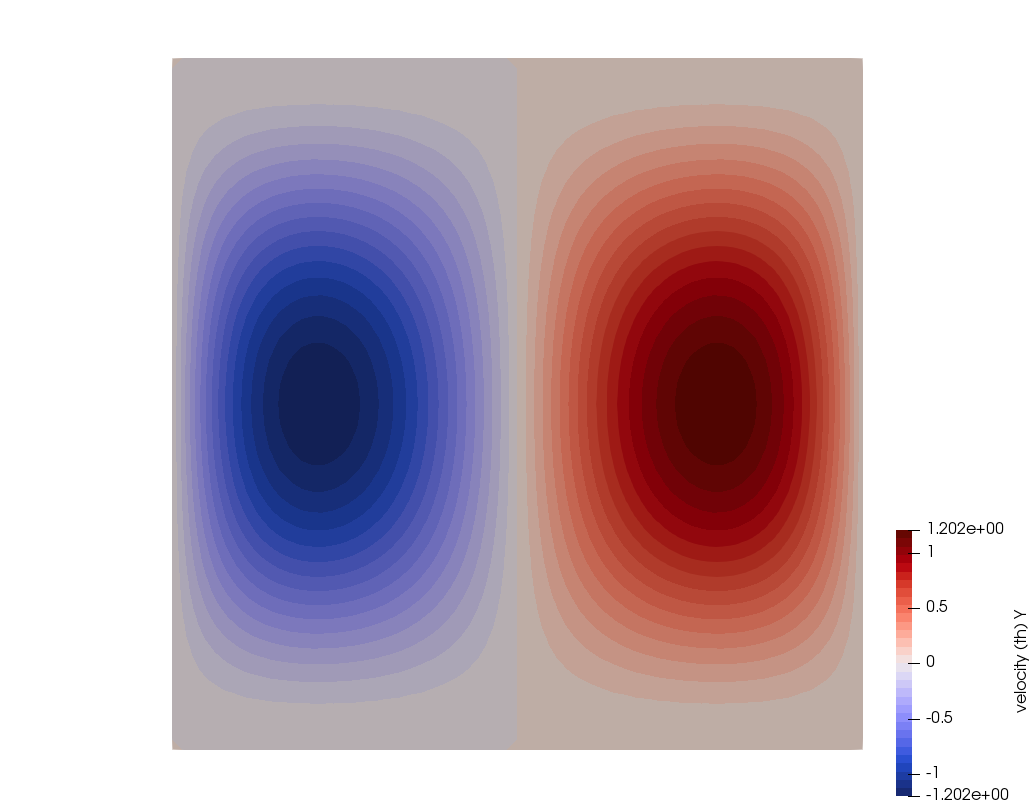
\includegraphics[width=4.5cm]{images/mms/vj3/v}
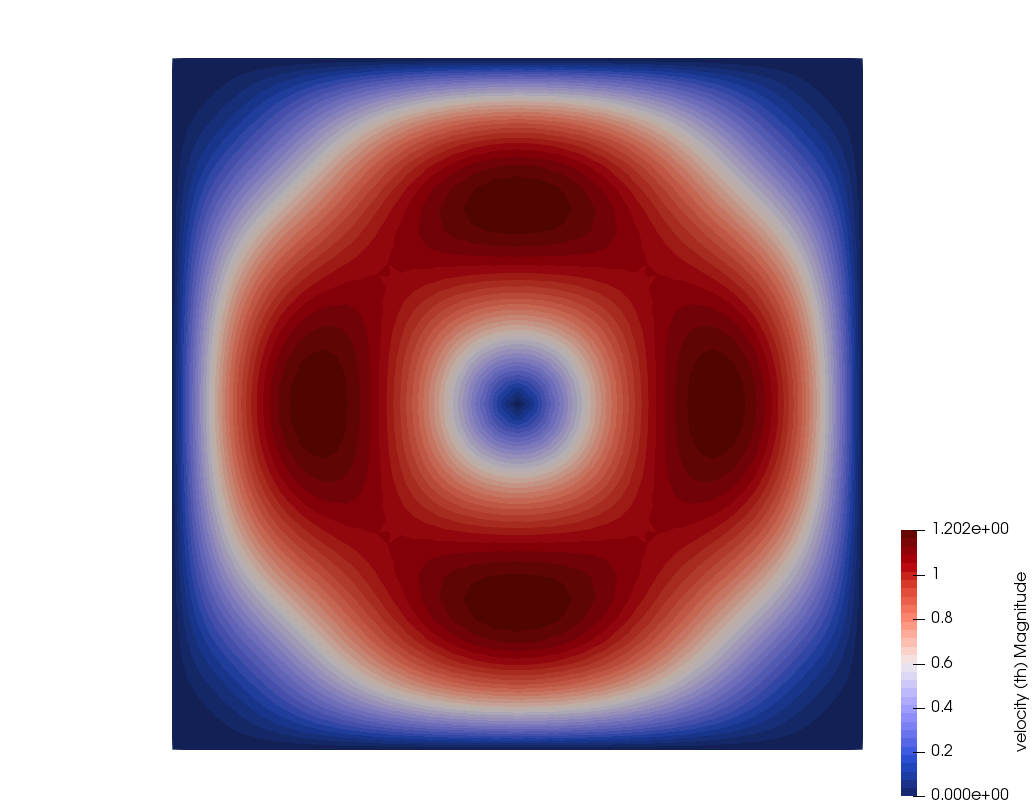
\includegraphics[width=4.5cm]{images/mms/vj3/vel}\\
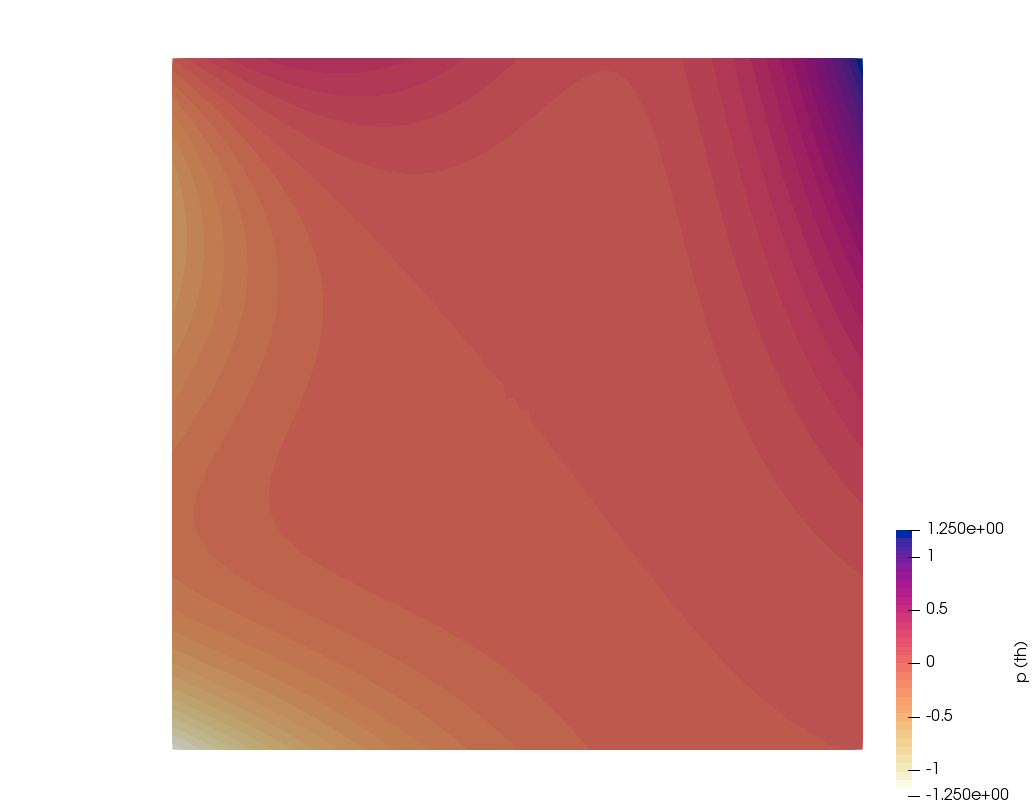
\includegraphics[width=4.5cm]{images/mms/vj3/p}
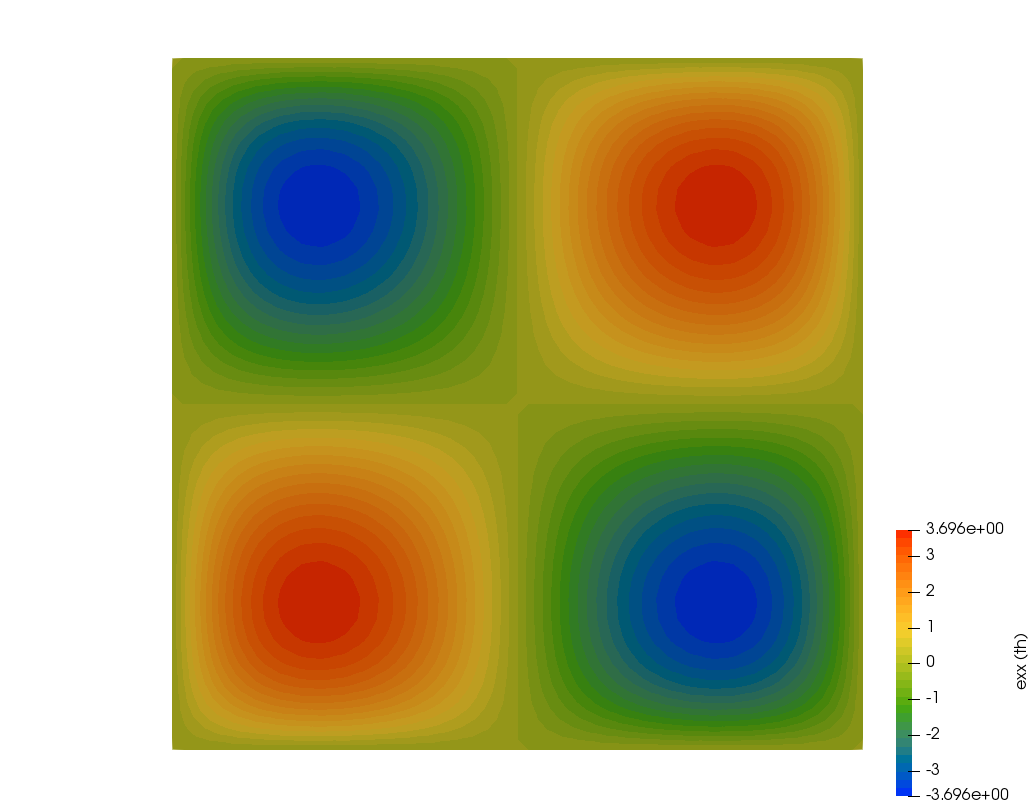
\includegraphics[width=4.5cm]{images/mms/vj3/exx}
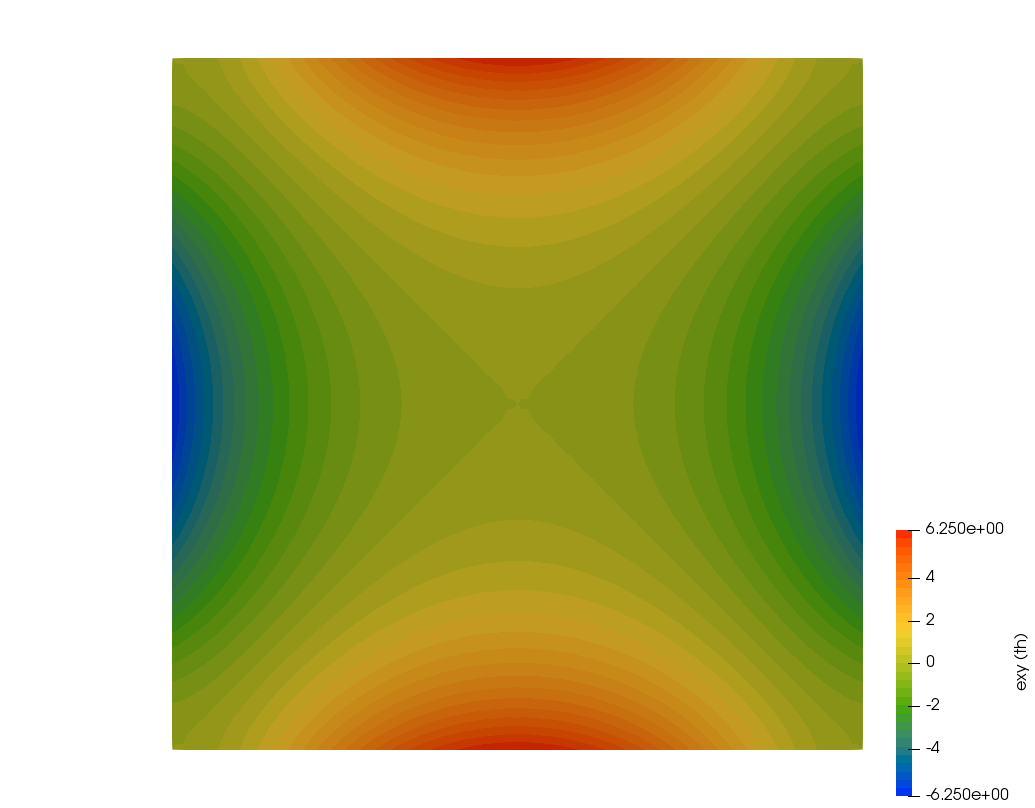
\includegraphics[width=4.5cm]{images/mms/vj3/exy}
\end{center}






 %----------------

\subsection{Assigning values to quadrature points}

As we have seen in Section \ref{solvingFEM}, the building of the elemental matrix and rhs
requires (at least) to assign a density and viscosity value to each quadrature point inside
the element. Depending on the type of modelling, this task can prove more complex than 
one might expect and have large consequences on the solution accuracy.

Here are several options:

\begin{itemize}
\item The simplest way (which is often used for benchmarks) consists in computing the 'real'
coordinates $(x_q,y_q,z_q)$ of a given quadrature point based on its reduced coordinates 
$(r_q,s_q,t_q)$, and passing these coordinates to a function which returns density and/or viscosity
at this location. For instance, for the Stokes sphere:
\begin{verbatim}
def rho(x,y):
    if (x-.5)**2+(y-0.5)**2<0.123**2:
       val=2.
    else:
       val=1.
    return val

def mu(x,y):
    if (x-.5)**2+(y-0.5)**2<0.123**2:
       val=1.e2
    else:
       val=1.
    return val
\end{verbatim}
This is very simple, but it has been shown to potentially be problematic. In essence, it can introduce very large contrasts inside a single element and perturb the quadrature. Please read section 3.3 of \cite{hedg17} and/or
have a look at the section titled "Averaging material properties" in the \aspect{} manual.

\item another similar approach consists in assigning a density and viscosity value to the nodes of the FE mesh first, and then using these nodal values to assign values to the quadrature points. Very often ,and quite logically, the basis functions are used to this effect. Indeed we have seen before that for any point $(r,s,t)$ inside an element we have
\[
f_h(r,s,t) = \sum_{i}^m f_i N_i(r,s,t)
\]  
where the $f_i$ are the nodal values and the $N_i$ the corresponding basis functions. 

In the case of linear elements ($Q_1$ basis functions), this is straightforward. In fact, the basis functions $N_i$ can be seen as moving weights: the closer the point is to a node, the higher the weight (basis function value). 

However, this is quite another story for quadratic elements ($Q_2$ basis functions). In order to illustrate the 
problem, let us consider a 1D problem. The basis functions are 
\[
N_1(r) =\frac{1}{2}r(r-1)
\quad\quad
N_2(r)=1-r^2
\quad\quad
N_3(r) =\frac{1}{2}r(r+1)
\]
Let us further assign: $\rho_1=\rho_2=0$ and $\rho_3=1$. Then 
\[
\rho_h(r) = \sum_{i}^m \rho_i N_i(r) = N_3(r)
\]  
There lies the core of the problem: the $N_3(r)$ basis function is negative for $r\in[-1,0]$. This means that the quadrature point in this interval will be assigned a negative density, which is nonsensical and numerically problematic!

{\color{red} use 2X Q1. write about it !}

\end{itemize}

The above methods work fine as long as the domain contains a single material. As soon as there are multiple fluids in the domain a special technique is needed to track either the fluids themselves or their interfaces. 
Let us start with markers. We are then confronted to the infernal trio (a {\it menage a trois}?)
which is present for each element, composed of its nodes, its markers and its quadrature points. 

Each marker carries the material information (density and viscosity). 
This information must ultimately be projected onto the quadrature points. Two main options are possible: an algorithm is designed and projects the marker-based fields onto the quadrature points directly or the marker fields are first projected onto the FE nodes and then onto the quadrature points using the techniques above.  

--------------------------




At a given time, every element $e$ contains $n^e$ markers. During the FE matrix building 
process, viscosity and density values are needed at the quadrature points. 
One therefore needs to project the values carried by the markers at these locations. 
Several approaches are currently in use in the community and the topic has been 
investigated 
by \cite{deka08} and \cite{dumg11} for instance.

{\sc elefant} adopts a simple approach: viscosity and density are considered to be elemental values, i.e. 
all the markers within a given element contribute to assign a unique constant density and viscosity 
value to the element by means of an averaging scheme. 

While it is common in the literature to treat the so-called arithmetic, geometric and harmonic means 
as separate averagings, I hereby wish to introduce the notion of generalised mean, which is a family 
of functions for aggregating sets of numbers that include as special cases the arithmetic, geometric and 
harmonic means. 

If $p$ is a non-zero real number, we can define the generalised mean (or power mean)
with exponent $p$ of the positive real numbers $a_1$, ... $a_n$ as:
\begin{equation}
M_p(a_1,...a_n)=
\left(
\frac{1}{n} \sum_{i=1}^n a_i^p
\right)^{1/p}
\end{equation}
and it is trivial to verify that we then have the special cases:
\begin{eqnarray}
M_{-\infty} &=& \lim_{p\rightarrow -\infty} M_p = \min (a_1,...a_n)                   \quad ({\rm minimum})  \\
M_{-1}      &=& \frac{n}{\frac{1}{a_1} + \frac{1}{a_2} + \cdots + \frac{1}{a_n}} \quad\quad  ({\rm harm.\; avrg.}) \\
M_{0}       &=& \lim_{p\rightarrow 0} M_p = \bigg(\prod_{i=1}^n a_i \bigg)^{1/n} \quad\quad  ({\rm geom.\; avrg.}) \\
M_{+1}      &=& \frac{1}{n}\sum_{i=1}^n a_i                                      \quad\quad\quad\quad\quad\quad  ({\rm arithm.\; avrg.}) \\
M_{+2}      &=& \sqrt{ \frac{1}{n} \sum_{i=1}^n a_i^2   }    \quad\quad\quad ({\rm root\;  mean \; square})  \\ 
M_{+\infty} &=& \lim_{p\rightarrow +\infty} M_p = \max (a_1,...a_n)     \quad ({\rm maximum}) 
\end{eqnarray}
Note that the proofs of the limit convergence are given in \cite{bull03}.  

An interesting property of the generalised mean is as follows:
for two real values $p$ and $q$, if $p<q$ then $M_p \leq M_q$.
This property has for instance been illustrated in Fig. 20 of \cite{scbe08}. 

One can then for instance look at the generalised mean of 
a randomly generated set of 1000 viscosity values within $10^{18}Pa.s$
and $10^{23}Pa.s$ for $-5\leq p\leq 5$. Results are shown 
in the figure hereunder and the arithmetic, geometric and 
harmonic values are indicated too. 
The function $M_p$ assumes an arctangent-like shape: very low values of p 
will ultimately yield the minimum viscosity in the array while very high values will 
yield its maximum. In between, the transition is smooth and occurs essentially for $|p|\leq 5$. 

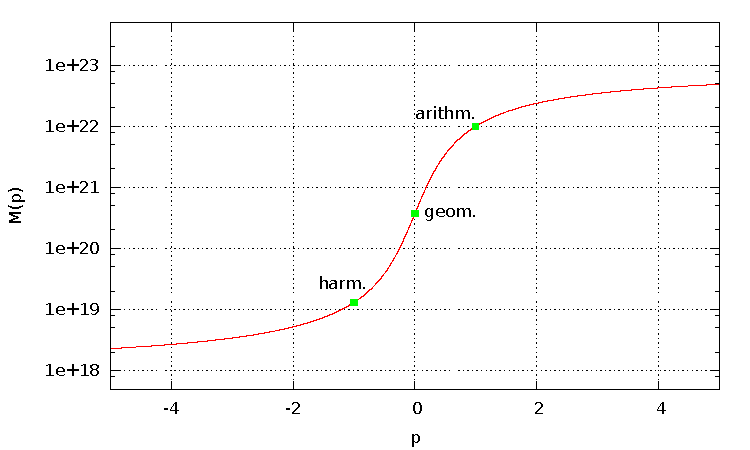
\includegraphics[width=12cm]{images/avrg/avrg.pdf}











\begin{mdframed}[backgroundcolor=green!5]
\begin{itemize}
\item[$\triangleright$] {\sl python\_codes/fieldstone\_markers\_avrg}
\end{itemize}
\end{mdframed}












 




\subsection{Picard and Newton}


\subsection{The SUPG formulation for the energy equation}

\subsection{Tracking materials and/or interfaces}

\subsection{Dealing with a free surface}

\newpage %---------------------------------------------------------------------
\subsection{Matrix (Sparse) storage} The FE matrix (or the blocks which compose it) 
is the result of the assembly process of all elemental matrices. 
Its size can become quite large when the resolution is being increased (from thousands
of lines/columns to tens of millions).

One important property of the matrix is its sparsity. Typically mush less than 1\% of the 
matrix terms is not zero and this means that the matrix storage can and {\it should} be optimised. 
Clever storage formats were designed early on since the amount of RAM memory in computers
was the limiting factor 3 or 4 decades ago \cite{saad}.

There are several standard formats, e.g.:
\begin{itemize}
\item compressed sparse row format (CSR) \index{general}{CSR} \index{general}{Compressed Sparse Row}
\item compressed sparse column format (CSC) \index{general}{CSC} \index{general}{Compressed Sparse Column}
\item the Coordinate Format (COO)
\item Skyline Storage Format
\end{itemize}

I focus on  the CSR format in what follows since it is the most common format 
and it is the one used in \elefant. 

%..............................................................................
\subsubsection{2D domain - One degree of freedom per node}

Let us consider again the  $3\times2$ element grid which counts 12 nodes.

\begin{center}
\begin{flushright} {\tiny {\color{gray} (tikz\_3x2.tex)}} \end{flushright}
%~~~~~~~~~~~~~~~~~~~~~~~~~~~~~~~~~~~~~~~~~~~~~~~~~~~~~~~~~~~~~~~~~~~~~~~~~~~~~~~~~~~~~~~~~~~~~~~~~~

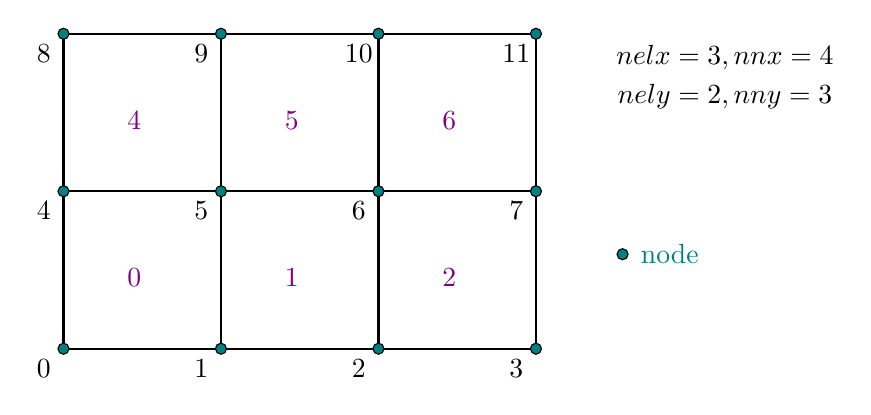
\begin{tikzpicture}
%\draw[step=0.5cm,gray,very thin] (0,0) grid (9,5); %background grid

\draw[thick] (1,1) -- (7,1) -- (7,5) -- (1,5) -- cycle;  
\draw[thick] (1,3) -- (7,3) ;
\draw[thick] (3,1) -- (3,5) ;
\draw[thick] (5,1) -- (5,5) ;

\draw[black,fill=teal] (1,1)     circle (2pt); 
\draw[black,fill=teal] (3,1)     circle (2pt); 
\draw[black,fill=teal] (5,1)     circle (2pt); 
\draw[black,fill=teal] (7,1)     circle (2pt); 

\draw[black,fill=teal] (1,3)     circle (2pt); 
\draw[black,fill=teal] (3,3)     circle (2pt); 
\draw[black,fill=teal] (5,3)     circle (2pt); 
\draw[black,fill=teal] (7,3)     circle (2pt); 

\draw[black,fill=teal] (1,5)     circle (2pt); 
\draw[black,fill=teal] (3,5)     circle (2pt); 
\draw[black,fill=teal] (5,5)     circle (2pt); 
\draw[black,fill=teal] (7,5)     circle (2pt); 

\node[] at (0.75,0.75) {0};
\node[] at (2.75,0.75) {1};
\node[] at (4.75,0.75) {2};
\node[] at (6.75,0.75) {3};

\node[] at (0.75,2.75) {4};
\node[] at (2.75,2.75) {5};
\node[] at (4.75,2.75) {6};
\node[] at (6.75,2.75) {7};

\node[] at (0.75,4.75) {8};
\node[] at (2.75,4.75) {9};
\node[] at (4.75,4.75) {10};
\node[] at (6.75,4.75) {11};

\node[violet] at (1.9,1.9) {0};
\node[violet] at (3.9,1.9) {1};
\node[violet] at (5.9,1.9) {2};
\node[violet] at (1.9,3.9) {4};
\node[violet] at (3.9,3.9) {5};
\node[violet] at (5.9,3.9) {6};

\draw[black,fill=teal] (8.1,2.2) circle (2pt); 
\node[] at (8.7,2.2) {{\color{teal}node}};

\node[] at (9.4,4.7) {$nelx=3, nnx=4$};
\node[] at (9.4,4.2) {$nely=2, nny=3$};

\end{tikzpicture}

\end{center}

\noindent In the case there is only a single degree of freedom per node, the 
assembled FEM matrix ${\bm M}$ will look like this:
\[
{\bm M}=
\left(
\begin{array}{cccccccccccc}
\Box & \Box &      &      & \Box & \Box &      &      &      &      &      &      \\
\Box & \Box & \Box &      & \Box & \Box & \Box &      &      &      &      &      \\
     & \Box & \Box & \Box &      & \Box & \Box & \Box &      &      &      &      \\
     &      & \Box & \Box &      &      & \Box & \Box &      &      &      &      \\
\Box & \Box &      &      & \Box & \Box &      &      & \Box & \Box &      &      \\
\Box & \Box & \Box &      & \Box & \Box & \Box &      & \Box & \Box & \Box &      \\
     & \Box & \Box & \Box &      & \Box & \Box & \Box &      & \Box & \Box & \Box \\
     &      & \Box & \Box &      &      & \Box & \Box &      &      & \Box & \Box \\
     &      &      &      & \Box & \Box &      &      & \Box & \Box &      &      \\
     &      &      &      & \Box & \Box & \Box &      & \Box & \Box & \Box &      \\
     &      &      &      &      & \Box & \Box & \Box &      & \Box & \Box & \Box \\
     &      &      &      &      &      & \Box & \Box &      &      & \Box & \Box 
\end{array}
\right)
\]
where the $\Box$ stand for non-zero terms.
This matrix structure stems from the fact that
\begin{itemize}
\item node 0 sees nodes 0,1,4,5 (1st line/column of the matrix)
\item node 1 sees nodes 0,1,2,4,5,6 (2nd line/column of the matrix)
\item node 2 sees nodes 1,2,3,5,6,7 (3rd line/column of the matrix)
\item node 3 sees nodes 2,3,6,7
\item node 4 sees nodes 0,1,4,5,8,9
\item node 5 sees nodes 0,1,2,4,5,6,8,9,10 
\item node 6 sees nodes 1,2,3,5,6,7,9,10,11
\item node 7 sees nodes 2,3,6,7,10,11
\item node 8 sees nodes 4,5,8,9
\item node 9 sees nodes 4,5,6,8,9,10
\item node 10 sees nodes 5,6,7,9,10,11 
\item node 11 sees nodes 6,7,10,11 (last line/column of the matrix)
\end{itemize}
In light thereof, we have
\begin{itemize}
\item 4 corner nodes which have 4 neighbours (counting themselves) 
\item 2(nnx-2) nodes which have 6 neighbours
\item 2(nny-2) nodes which have 6 neighbours
\item (nnx-2)$\times$(nny-2) nodes which have 9 neighbours
\end{itemize}
In total, the number of non-zero terms in the matrix above is then:
\[
NZ=4\times4+4\times6+2\times6+2\times9=70
\]
and in general, we would then have:
\[
NZ=4\times4+[2(nnx-2)+2(nny-2)]\times6 + (nnx-2)(nny-2)\times9
\]
Let us temporarily assume $nnx=nny=n$. The matrix size (total
number of unknowns) is then $N=n^2$ and  
\[
NZ=16+24(n-2)+9(n-2)^2
\]
A full matrix array would contain $N^2=n^4$ terms. 
The ratio of $NZ$ (the actual number of reals to store)
to the full matrix size (the number of reals a full matrix contains) is then 
\[
R = \frac{16+24(n-2)+9(n-2)^2}{n^4}
\]
It is then obvious that when $n$ is large enough $R \sim 1/n^2$.

CSR stores the nonzeros of the matrix row by row, in a
single indexed array A of double precision  numbers.
Another array COLIND contains the column index of each
corresponding entry in the A array. A third integer array RWPTR
contains pointers to the beginning of each row, which an additional pointer to
the first index following the nonzeros of the matrix A.
A and COLIND have length NZ and RWPTR has length N+1.

In the case of the here-above matrix, the arrays COLIND and RWPTR will look like:
\begin{eqnarray}
COLIND&=&(0,1,4,5, \; 0,1,2,4,5,6, \; 1,2,3,5,6,7, ..., 6,7,10,11) \nn\\
RWPTR &=&(0,4,10,16, ... )   \nn
\end{eqnarray}

%..............................................................................
\subsubsection{2D domain - Symmetric matrix CSR storage}

If the matrix is symmetric, i.e. ${\bm M}={\bm M}^T$, then we may wish to 
only store half of it, always in the interest of saving memory. 
Only the following remaining $\Box$ entries are relevant now:
\[
{\bm M}=
\left(
\begin{array}{cccccccccccc}
\Box & \Box &      &      & \Box & \Box &      &      &      &      &      &      \\
     & \Box & \Box &      & \Box & \Box & \Box &      &      &      &      &      \\
     &      & \Box & \Box &      & \Box & \Box & \Box &      &      &      &      \\
     &      &      & \Box &      &      & \Box & \Box &      &      &      &      \\
     &      &      &      & \Box & \Box &      &      & \Box & \Box &      &      \\
     &      &      &      &      & \Box & \Box &      & \Box & \Box & \Box &      \\
     &      &      &      &      &      & \Box & \Box &      & \Box & \Box & \Box \\
     &      &      &      &      &      &      & \Box &      &      & \Box & \Box \\
     &      &      &      &      &      &      &      & \Box & \Box &      &      \\
     &      &      &      &      &      &      &      &      & \Box & \Box &      \\
     &      &      &      &      &      &      &      &      &      & \Box & \Box \\
     &      &      &      &      &      &      &      &      &      &      & \Box 
\end{array}
\right)
\]
We see that the number of nonzeros is now 
\[
NZ_{symm}= \frac{NZ-n}{2}+n
\]
and in this case $NZ_{symm}=(70-12)/2+12=41$.
Then 
\begin{eqnarray}
COLIND&=&(0,1,4,5, \; 1,2,4,5,6, \; 3,5,6,7, ..., ,11) \nn\\
RWPTR &=&(0,4,9,14, ... )   \nn
\end{eqnarray}


%..............................................................................
\subsubsection{2D domain - Two degrees of freedom per node}

When there are now two degrees of freedom per node, such as in the case of the Stokes equation
in two-dimensions, the size of the $\K$ matrix is given $NfemV=nnx*nny*ndofV$  
where $NfemV$ is the total number of velocity degrees of freedom.

\begin{center}
\begin{flushright} {\tiny {\color{gray} (tikz\_3x2\_two.tex)}} \end{flushright}
%~~~~~~~~~~~~~~~~~~~~~~~~~~~~~~~~~~~~~~~~~~~~~~~~~~~~~~~~~~~~~~~~~~~~~~~~~~~~~~~~~~~~~~~~~~~~~~~~~~


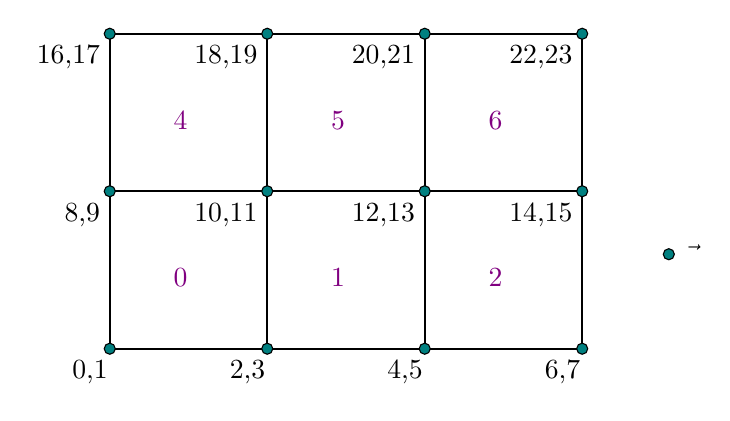
\begin{tikzpicture}
%\draw[step=0.5cm,gray,very thin] (0,0) grid (5,5); %background grid

\draw[thick] (1,1) -- (7,1) -- (7,5) -- (1,5) -- cycle;  
\draw[thick] (1,3) -- (7,3) ;
\draw[thick] (3,1) -- (3,5) ;
\draw[thick] (5,1) -- (5,5) ;

\draw[black,fill=teal] (1,1)     circle (2pt); 
\draw[black,fill=teal] (3,1)     circle (2pt); 
\draw[black,fill=teal] (5,1)     circle (2pt); 
\draw[black,fill=teal] (7,1)     circle (2pt); 

\draw[black,fill=teal] (1,3)     circle (2pt); 
\draw[black,fill=teal] (3,3)     circle (2pt); 
\draw[black,fill=teal] (5,3)     circle (2pt); 
\draw[black,fill=teal] (7,3)     circle (2pt); 

\draw[black,fill=teal] (1,5)     circle (2pt); 
\draw[black,fill=teal] (3,5)     circle (2pt); 
\draw[black,fill=teal] (5,5)     circle (2pt); 
\draw[black,fill=teal] (7,5)     circle (2pt); 

\node[] at (0.75,0.7) {0,1};
\node[] at (2.75,0.7) {2,3};
\node[] at (4.75,0.7) {4,5};
\node[] at (6.75,0.7) {6,7};

\node[] at (0.65,2.7) {8,9};
\node[] at (2.475,2.7) {10,11};
\node[] at (4.475,2.7) {12,13};
\node[] at (6.475,2.7) {14,15};

\node[] at (0.475,4.7) {16,17};
\node[] at (2.475,4.7) {18,19};
\node[] at (4.475,4.7) {20,21};
\node[] at (6.475,4.7) {22,23};

\node[violet] at (1.9,1.9) {0};
\node[violet] at (3.9,1.9) {1};
\node[violet] at (5.9,1.9) {2};
\node[violet] at (1.9,3.9) {4};
\node[violet] at (3.9,3.9) {5};
\node[violet] at (5.9,3.9) {6};

\draw[black,fill=teal] (8.1,2.2) circle (2pt); 
\node[] at (8.4,2.2) {$\vec\upnu$};

\end{tikzpicture}





\end{center}

In the case of the small grid above, we have then $NfemV=24$ and
elemental matrices are now $8\times8$ in size.

We still have
\begin{itemize}
\item $4$ corner nodes which have 4 neighbours
\item $2(nnx-2)$ nodes which have 6 neighbours
\item $2(nny-2)$ nodes which have 6 neighbours
\item $(nnx-2)\cdot(nny-2)$ nodes which have 9 neighbours,
\end{itemize}
but now each degree of freedom from a node sees the other two
degrees of freedom of another node too.
In that case, the number of nonzeros has been multiplied by four
and the assembled FEM matrix looks like:
\begin{equation}
\left(
\begin{array}{cccccccccccccccccccccccc}
\Box&\Box & \Box&\Box &  &  &  &  & \Box&\Box & \Box&\Box &  &  &  &  &  &  &  &  &  &  &  &  \\
\Box&\Box & \Box&\Box &  &  &  &  & \Box&\Box & \Box&\Box &  &  &  &  &  &  &  &  &  &  &  &  \\
\Box&\Box & \Box&\Box & \Box&\Box &  &  & \Box&\Box & \Box&\Box & \Box&\Box &  &  &  &  &  &  &  &  &  &  \\
\Box&\Box & \Box&\Box & \Box&\Box &  &  & \Box&\Box & \Box&\Box & \Box&\Box &  &  &  &  &  &  &  &  &  &  \\
 &  & \Box&\Box & \Box&\Box & \Box&\Box &  &  & \Box&\Box & \Box&\Box & \Box&\Box &  &  &  &  &  &  &  &  \\
 &  & \Box&\Box & \Box&\Box & \Box&\Box &  &  & \Box&\Box & \Box&\Box & \Box&\Box &  &  &  &  &  &  &  &  \\
 &  &  &  & \Box&\Box & \Box&\Box &  &  &  &  & \Box&\Box & \Box&\Box &  &  &  &  &  &  &  &  \\
 &  &  &  & \Box&\Box & \Box&\Box &  &  &  &  & \Box&\Box & \Box&\Box &  &  &  &  &  &  &  &  \\
\Box&\Box & \Box&\Box &  &  &  &  & \Box&\Box & \Box&\Box &  &  &  &  & \Box&\Box & \Box&\Box &  &  &  &  \\
\Box&\Box & \Box&\Box &  &  &  &  & \Box&\Box & \Box&\Box &  &  &  &  & \Box&\Box & \Box&\Box &  &  &  &  \\
\Box&\Box & \Box&\Box & \Box&\Box &  &  & \Box&\Box & \Box&\Box & \Box&\Box &  &  & \Box&\Box & \Box&\Box & \Box&\Box &  &  \\
\Box&\Box & \Box&\Box & \Box&\Box &  &  & \Box&\Box & \Box&\Box & \Box&\Box &  &  & \Box&\Box & \Box&\Box & \Box&\Box &  &  \\
 &  & \Box&\Box & \Box&\Box & \Box&\Box &  &  & \Box&\Box & \Box&\Box & \Box&\Box &  &  & \Box&\Box & \Box&\Box & \Box&\Box \\
 &  & \Box&\Box & \Box&\Box & \Box&\Box &  &  & \Box&\Box & \Box&\Box & \Box&\Box &  &  & \Box&\Box & \Box&\Box & \Box&\Box \\
 &  &  &  & \Box&\Box & \Box&\Box &  &  &  &  & \Box&\Box & \Box&\Box &  &  &  &  & \Box&\Box & \Box&\Box \\
 &  &  &  & \Box&\Box & \Box&\Box &  &  &  &  & \Box&\Box & \Box&\Box &  &  &  &  & \Box&\Box & \Box&\Box \\
 &  &  &  &  &  &  &  & \Box&\Box & \Box&\Box &  &  &  &  & \Box&\Box & \Box&\Box &  &  &  &  \\
 &  &  &  &  &  &  &  & \Box&\Box & \Box&\Box &  &  &  &  & \Box&\Box & \Box&\Box &  &  &  &  \\
 &  &  &  &  &  &  &  & \Box&\Box & \Box&\Box & \Box&\Box &  &  & \Box&\Box & \Box&\Box & \Box&\Box &  &  \\
 &  &  &  &  &  &  &  & \Box&\Box & \Box&\Box & \Box&\Box &  &  & \Box&\Box & \Box&\Box & \Box&\Box &  &  \\
 &  &  &  &  &  &  &  &  &  & \Box&\Box & \Box&\Box & \Box&\Box &  &  & \Box&\Box & \Box&\Box & \Box&\Box \\
 &  &  &  &  &  &  &  &  &  & \Box&\Box & \Box&\Box & \Box&\Box &  &  & \Box&\Box & \Box&\Box & \Box&\Box \\
 &  &  &  &  &  &  &  &  &  &  &  & \Box&\Box & \Box&\Box &  &  &  &  & \Box&\Box & \Box&\Box \\
 &  &  &  &  &  &  &  &  &  &  &  & \Box&\Box & \Box&\Box &  &  &  &  & \Box&\Box & \Box&\Box 
\end{array}
\right)\nonumber
\end{equation}
Note that the degrees of freedom are organised as follows: 
\[
(u_0,v_0,u_1,v_1,u_2,v_2, ... u_{11},v_{11})
\]
In general, we would then have:
\[
NZ=4 \left[4\times4+[2(nnx-2)+2(nny-2)]\times6 + (nnx-2)(nny-2)\times9 \right]
\]
and in the case of the small grid,
the number of non-zero terms in the matrix is then:
\[
NZ=4\left[4\times4+4\times6+2\times6+2\times9\right]=280
\]
In the case of the here-above matrix, the arrays COLIND and RWPTR will look like:
\begin{eqnarray}
COLIND&=&(0,1,2,3,8,9,10,11, \; 0,1,2,3,8,9,10,11,\; ...) \nn\\
RWPTR &=&(0,8,16,28, ... ) \nn
\end{eqnarray}


%..............................................................................
\subsubsection{3D domain - CSR- Three degrees of freedom}


Let us consider a $3\times4\times2$ grid which counts 
$nnx\cdot nny \cdot nnz = 5 \cdot 4\cdot 3=60$ nodes.
The assembled FEM matrix $\K$ size is then 
$N=nnx\times nny\times nnz \times ndof=180$.

\begin{center}
\begin{flushright} {\tiny {\color{gray} (tikz\_4x3x2.tex)}} \end{flushright}
%~~~~~~~~~~~~~~~~~~~~~~~~~~~~~~~~~~~~~~~~~~~~~~~~~~~~~~~~~~~~~~~~~~~~~~~~~~~~~~~~~~~~~~~~~~~~~~~~~~


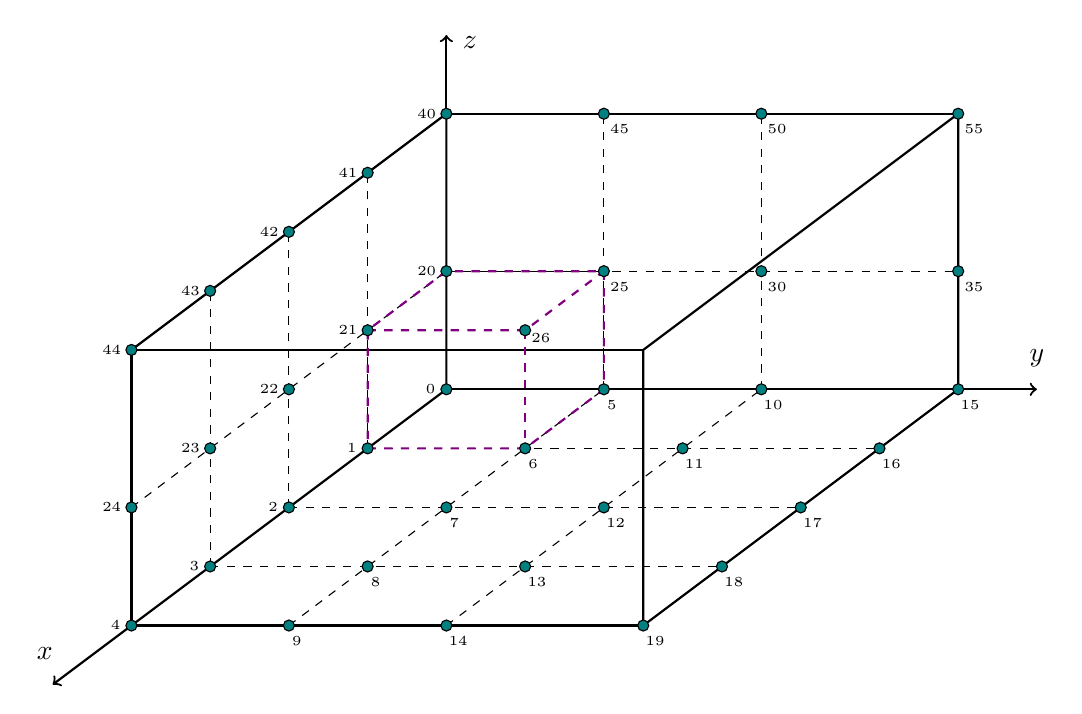
\begin{tikzpicture}
%\draw[step=0.5cm,gray,very thin] (0,0) grid (14,10); %background grid

%element
\draw[thick] (2,2) -- (8.5,2) -- (8.5,5.5) -- (2,5.5) -- cycle;  
\draw[thick] (2,2) -- (6,5) -- (6,8.5) -- (2,5.5) -- cycle ;
\draw[thick] (8.5,2) -- (12.5,5) -- (12.5,8.5) -- (8.5,5.5) -- cycle ;
\draw[thick] (6,5) -- (12.5,5) ;
\draw[thick] (6,8.5) -- (12.5,8.5) ;

%axes
\draw[thick,->] (2,2)--(1,1.25);
\draw[thick,->] (12.5,5)--(13.5,5);
\draw[thick,->] (6,8.5)--(6,9.5);
\node[] at (0.9,1.65) {$x$};
\node[] at (13.5,5.4) {$y$};
\node[] at (6.3,9.4) {$z$};

\draw[dashed] (2,3.5)--(6,6.5);
\draw[dashed] (3,2.75)--(3,6.25);
\draw[dashed] (4,3.5)--(4,7);
\draw[dashed] (5,4.25)--(5,7.75);
\draw[dashed] (4,2)--(8,5);
\draw[dashed] (6,2)--(10,5);
\draw[dashed] (3,2.75)--(9.5,2.75);
\draw[dashed] (4,3.5)--(10.5,3.5);
\draw[dashed] (5,4.25)--(11.5,4.25);
\draw[dashed] (6,6.5)--(12.5,6.5);
\draw[dashed] (8,5)--(8,8.5);
\draw[dashed] (10,5)--(10,8.5);

\draw[dashed, thick,violet] (5,4.25)--(7,4.25) --(8,5)--(8,6.5) --(6,6.5)--(5,5.75)--(5,4.25);
\draw[dashed, thick,violet] (5,5.75)--(7,5.75)--(8,6.5);
\draw[dashed, thick,violet] (7,5.75)--(7,4.25);

\draw[black,fill=teal] (2,2) circle (2pt); 
\draw[black,fill=teal] (3,2.75) circle (2pt); 
\draw[black,fill=teal] (4,3.5) circle (2pt); 
\draw[black,fill=teal] (5,4.25) circle (2pt); 
\draw[black,fill=teal] (6,5) circle (2pt); 

\draw[black,fill=teal] (2,3.5) circle (2pt); 
\draw[black,fill=teal] (3,4.25) circle (2pt); 
\draw[black,fill=teal] (4,5) circle (2pt); 
\draw[black,fill=teal] (5,5.75) circle (2pt); 
\draw[black,fill=teal] (6,6.5) circle (2pt); 

\draw[black,fill=teal] (2,5.5) circle (2pt); 
\draw[black,fill=teal] (3,6.25) circle (2pt); 
\draw[black,fill=teal] (4,7) circle (2pt); 
\draw[black,fill=teal] (5,7.75) circle (2pt); 
\draw[black,fill=teal] (6,8.5) circle (2pt); 

\draw[black,fill=teal] (4,2) circle (2pt); 
\draw[black,fill=teal] (5,2.75) circle (2pt); 
\draw[black,fill=teal] (6,3.5) circle (2pt); 
\draw[black,fill=teal] (7,4.25) circle (2pt); 
\draw[black,fill=teal] (8,5) circle (2pt); 

\draw[black,fill=teal] (6,2) circle (2pt); 
\draw[black,fill=teal] (7,2.75) circle (2pt); 
\draw[black,fill=teal] (8,3.5) circle (2pt); 
\draw[black,fill=teal] (9,4.25) circle (2pt); 
\draw[black,fill=teal] (10,5) circle (2pt); 

\draw[black,fill=teal] (8.5,2) circle (2pt); 
\draw[black,fill=teal] (9.5,2.75) circle (2pt); 
\draw[black,fill=teal] (10.5,3.5) circle (2pt); 
\draw[black,fill=teal] (11.5,4.25) circle (2pt); 
\draw[black,fill=teal] (12.5,5) circle (2pt);

\draw[black,fill=teal] (7,5.75) circle (2pt);


\draw[black,fill=teal] (8,6.5) circle (2pt);
\draw[black,fill=teal] (8,8.5) circle (2pt);

\draw[black,fill=teal] (10,6.5) circle (2pt);
\draw[black,fill=teal] (10,8.5) circle (2pt);

\draw[black,fill=teal] (12.5,6.5) circle (2pt);
\draw[black,fill=teal] (12.5,8.5) circle (2pt);

\node[] at (5.8,5) {\tiny 0};
\node[] at (4.8,4.25) {\tiny 1};
\node[] at (3.8,3.5) {\tiny 2};
\node[] at (2.8,2.75) {\tiny 3};
\node[] at (1.8,2) {\tiny 4};

\node[] at (5.75,6.5) {\tiny 20};
\node[] at (4.75,5.75) {\tiny 21};
\node[] at (3.75,5) {\tiny 22};
\node[] at (2.75,4.25) {\tiny 23};
\node[] at (1.75,3.5) {\tiny 24};

\node[] at (5.75,8.5) {\tiny 40};
\node[] at (4.75,7.75) {\tiny 41};
\node[] at (3.75,7) {\tiny 42};
\node[] at (2.75,6.25) {\tiny 43};
\node[] at (1.75,5.5) {\tiny 44};

\node[] at (8.1,4.8) {\tiny 5};
\node[] at (7.1,4.05) {\tiny 6};
\node[] at (6.1,3.3) {\tiny 7};
\node[] at (5.1,2.55) {\tiny 8};
\node[] at (4.1,1.8) {\tiny 9};

\node[] at (10.15,4.8) {\tiny 10};
\node[] at (9.15,4.05) {\tiny 11};
\node[] at (8.15,3.3) {\tiny 12};
\node[] at (7.15,2.55) {\tiny 13};
\node[] at (6.15,1.8) {\tiny 14};

\node[] at (12.65,4.8) {\tiny 15};
\node[] at (11.65,4.05) {\tiny 16};
\node[] at (10.65,3.3) {\tiny 17};
\node[] at (9.65,2.55) {\tiny 18};
\node[] at (8.65,1.8) {\tiny 19};

\node[] at (8.2,6.3) {\tiny 25};
\node[] at (7.2,5.65) {\tiny 26};

\node[] at (8.2,8.3) {\tiny 45};
\node[] at (10.2,6.3) {\tiny 30};
\node[] at (10.2,8.3) {\tiny 50};

\node[] at (12.7,6.3) {\tiny 35};
\node[] at (12.7,8.3) {\tiny 55};

\end{tikzpicture}

\end{center}



The total number of nonzeros in the case $ndof=1$ would be decomposed as follows:
\begin{itemize}
\item 8 corners 'see' 8 neighbours
\item 4 edges with $(nnx-2)$ nodes in the x direction see 12 nodes
\item 4 edges with $(nny-2)$ nodes in the y direction see 12 nodes
\item 4 edges with $(nnz-2)$ nodes in the z direction see 12 nodes
\item $2(nnx-2)(nny-2)$ nodes see 18 nodes
\item $2(nnx-2)(nnz-2)$ nodes see 18 nodes
\item $2(nny-2)(nnz-2)$ nodes see 18 nodes
\item $(nnx-2)(nny-2)(nnz-2)$ interior nodes see 27 nodes
\end{itemize}





%..............................................................................
\subsubsection{Matrix Storage in fieldstone}

The majority of the codes have the FE matrix being a full array
\begin{lstlisting}
a_mat = np.zeros((Nfem,Nfem),dtype=np.float64) 
\end{lstlisting}
and it is converted to CSR format on the fly in the solve phase:
\begin{lstlisting}
sol = sps.linalg.spsolve(sps.csr_matrix(a_mat),rhs)
\end{lstlisting}

Note that linked list storages can be used (lil\_matrix). Substantial memory savings 
but much longer compute times since it takes longer to write in such arrays.
A conversion to CSR format is still necessary before calling the solver.




%..............................................................................
\subsubsection{Sparse Matrix-Vector multiplication}
\index{general}{SpMV} \index{general}{Sparse Matrix-Vector Multiplication}

When/if the matrix ${\bm M}$ is stored in a two-dimensional array, 
its (left or right) multiplication by a vector is trivial. 
Either one resorts to writing a double for loop (not recommended), 
either one uses {\tt numpy.dot}\footnote{\url{https://numpy.org/doc/stable/reference/generated/numpy.dot.html}}
in python, or {\tt matmul} in Fortran.

However, when the matrix is stored as a single continuous array, say CSR, how does this work?
This question is {\it very important} since iterative solvers such as the Conjugate Gradient solver
(see Section~\ref{ss:itsolvers}) rely extensively on multiplying the matrix by many different vectors. 

The Sparse Matrix-Vector multiplication operation is often abbreviated SpMV.
To quote Knepley \cite{knepley}: "The Sparse Matrix-Vector Product (SpMV) is today 
a workhorse of scientific computing. It is a central kernel is iterative linear and 
nonlinear solvers for PDE, and now for many graph algorithms."
As explained in Williams \etal (2007) \cite{wiov07} (and in many 
other sources on the topic), the algorithm for 
a basic SpMV implementation is rather simple in its naive form. 

\begin{center}
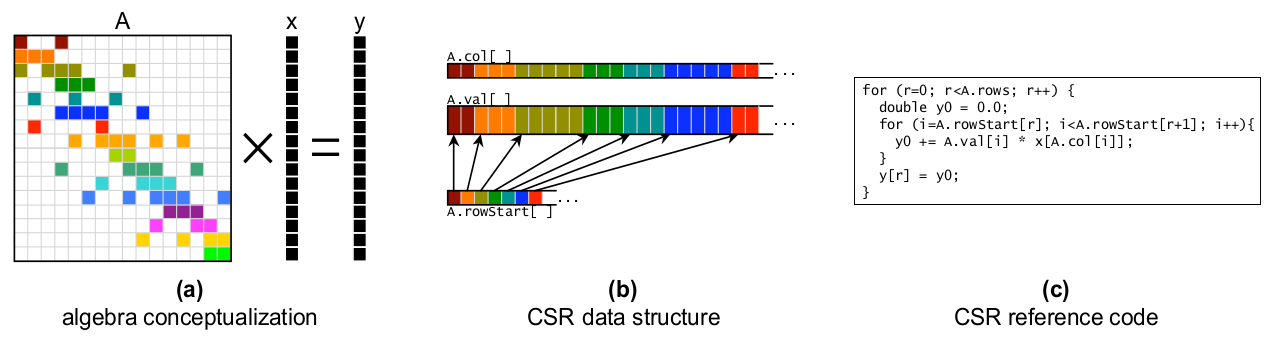
\includegraphics[width=17cm]{images/spmv/widc08}\\
{\captionfont Taken from Williams \etal (2008) \cite{widc08}. 
Sparse Matrix Vector Multiplication (SpMV). 
(a) visualization of the algebra: $\vec{y} \leftarrow {\bm A}\cdot \vec{x}$.\\
(b) Standard compressed sparse row (CSR) representation of the matrix.  \\
(c) The standard implementation of SpMV for a matrix stored in CSR. 
The outer loop is trivially parallelized without any data dependencies.}
\end{center}

Let us assume that we wish to compute $\vec{y}={\bm A}\cdot \vec{x}$ where ${\bm A}$ 
is in CSR format. The pseudo code then goes as follows:
\begin{verbatim}
for i in range(0,m):
    y0=0
    for k in range(ROWPTR[i],ROWPTR[i+1]):
        y0 += VAL[k] * x[COLIND[k]]
    y[i]=y0
\end{verbatim} 
Although technically correct, this algorithm is problematic because the vector x array
is accessed indirectly and this causes a non-optimal use of the processor, which 
in the end makes the calculation take longer than it should.


The following piece of code comes from \elefant. Note that here (ROWPTR=ia, COLIND=ja, VAL=mat)
\begin{lstlisting}[language=Fortran]
subroutine spmv (nr,nc,nz,x,y,mat,ja,ia)
implicit none
integer, intent(in)  :: nr,nc,nz
real(8), intent(in)  :: x(nc), mat(nz)
real(8), intent(out) :: y(nr)
integer, intent(in)  :: ja(nz),ia(nr+1)
real(8) t
integer i, k

do i = 1,nr
   t = 0.0d0
   do k=ia(i), ia(i+1)-1
      t = t + mat(k)*x(ja(k))
   end do
   y(i) = t 
end do

end subroutine
\end{lstlisting}


How to make this calculation as efficiently as possible on CPUs and GPUs, on one thread 
or multiple threads has given rise to a lot of literature.

\Literature Krotkiewski \& Dabrowski \cite{krda10}, Section 9.4 of Kepley \cite{knepley}, 
Williams \etal (2008) \cite{widc08}

 %-------------------------

\newpage %---------------------------------------------------------------------
\subsection{Mesh generation} \label{subsection_meshes} \begin{flushright} {\tiny {\color{gray} meshes.tex}} \end{flushright}
%~~~~~~~~~~~~~~~~~~~~~~~~~~~~~~~~~~~~~~~~~~~~~~~~~~~~~~~~~~~~~~~~~~~~~~~~~~~~~~~~~~~~~~~~~~~~~~~~~~

Before basis functions can be defined and PDEs can be discretised and solved 
we must first tesselate the domain with polygons, e.g. triangles and 
quadrilaterals in 2D, tetrahedra, prisms and hexahedra in 3D. \index{general}{Convex Polygon} 

When the domain is itself simple (e.g. a rectangle, a sphere, ...) the mesh (or grid) can 
be (more or less) easily produced and the connectivity array filled with straightforward 
algorithms \cite{thie18}.
However, real life applications can involve extremely complex geometries (e.g. a bridge, 
a human spine, a car chassis and body, etc ...) and dedicated algorithms/softwares 
must be used (see \cite{thsw,frge,xiyz09}). 

We usually distinguish between two broad classes of grids: structured grids (with a regular 
connectivity) and unstructured grids (with an irregular connectivity).
\index{general}{Structured Grid} \index{general}{Unstructured Grid}

\begin{center}
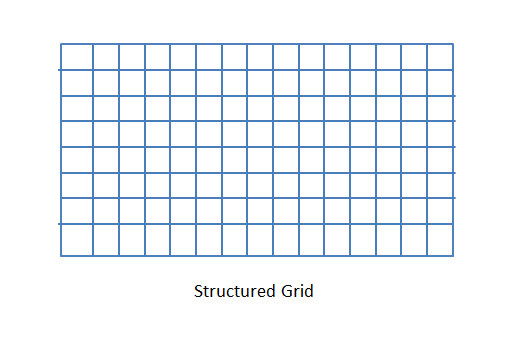
\includegraphics[width=5cm]{images/meshes/structured_grid}
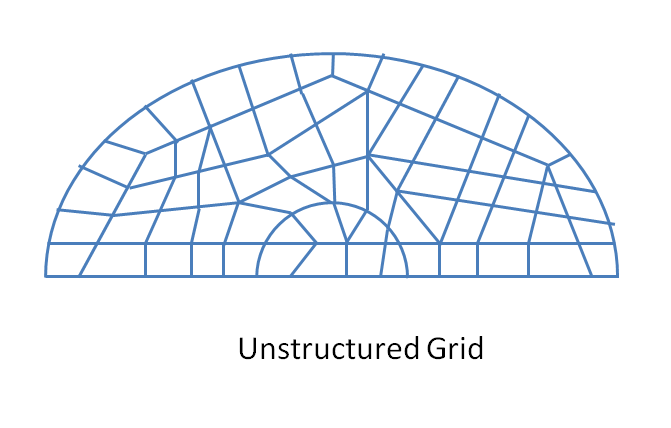
\includegraphics[width=5cm]{images/meshes/unstructured_grid}
\end{center}

\begin{remark}
\index{general}{Meshless}
Various families of so-called meshless methods exist and are commonly employed in Computational 
Fluid Dynamics \cite{liugu,liliu,grliu,liuliu}. They are however very rarely used in 
Computational geodynamics, with a noticeable exception \cite{hans03}.
\end{remark}

%............................................
\subsubsection{Quadrilateral-based meshes}

Let us now focus on the case of a rectangular computational domain of size 
{\tt Lx} $\times$ {\tt Ly} with a regular mesh composed of {\tt nelx}$\times${\tt nely}={\tt nel}
   quadrilaterals.  
There are then {\tt nnx}$\times${\tt nny}={\tt nnp} grid points.
The elements are of size {\tt hx}$\times${\tt hy} with {\tt hx}={\tt Lx}/{\tt nelx}.

We have no reason to come up with an irregular/illogical node numbering so 
we can number nodes row by row or column by column as shown on the example 
hereunder of a 3$\times$2 grid:

\begin{verbatim}
8=======9======10======11       2=======5=======8======11
|       |       |       |       |       |       |       |
|  (3)  |  (4)  |  (5)  |       |  (1)  |  (3)  |  (5)  |
|       |       |       |       |       |       |       |
4=======5=======6=======7       1=======4=======7======10
|       |       |       |       |       |       |       |
|  (0)  |  (1)  |  (2)  |       |  (0)  |  (2)  |  (4)  |
|       |       |       |       |       |       |       |
0=======1=======2=======3       0=======3=======6=======9

     "row by row"                  "column by column"
\end{verbatim}

The numbering of the elements themselves could be done in a somewhat chaotic 
way but we follow the numbering of the nodes for simplicity.
The row by row option is the adopted one in \fieldstone{} and the coordinates of the 
points are computed as follows:

\begin{lstlisting}
x = np.empty(nnp, dtype=np.float64)
y = np.empty(nnp, dtype=np.float64)
counter = 0
for j in range(0,nny):
    for i in range(0,nnx):
        x[counter]=i*hx
        y[counter]=j*hy
        counter += 1
\end{lstlisting}
The inner loop has {\tt i} ranging from {\tt 0} to {\tt nnx-1} first for {\tt j}=0, 1, ...
up to {\tt nny-1} which indeed corresponds to the row by row numbering.

\index{general}{Connectivity Array} 
We now turn to the connectivity. As mentioned before, this is a structured mesh so that the so-called
connectivity array, named {\tt icon} in our case, can be filled easily. For each element we need
to store the node identities of its vertices. Since there are {\tt nel} elements and {\tt m=4} corners, 
this is a {\tt m}$\times${\tt nel} array. The algorithm goes as follows:

\begin{lstlisting}
icon =np.zeros((m,nel),dtype=np.int16)
counter = 0
for j in range(0,nely):
    for i in range(0,nelx):
        icon[0,counter] = i + j * nnx 
        icon[1,counter] = i + 1 + j * nnx 
        icon[2,counter] = i + 1 + (j + 1) * nnx 
        icon[3,counter] = i + (j + 1) * nnx 
        counter += 1
\end{lstlisting}

In the case of the 3$\times$2 mesh, the {\tt icon} is filled as follows:
\begin{center}
\begin{tabular}{ccccccc}
element id$\rightarrow$ &0 &1&2&3&4&5 \\
node id$\downarrow$ \\
0& 0& 1& 2& 4& 5  &6\\
1& 1& 2& 3& 5& 6  &7\\
2& 5& 6& 7& 9& 10 &11\\
3& 4& 5& 6& 8& 9  &10\\
\end{tabular}
\end{center}
It is to be understood as follows: element $\#4$ is composed of nodes 5, 6, 10 and 9.
Note that nodes are always stored in a counter clockwise manner, starting at the bottom left.
This is very important since the corresponding basis functions and their derivatives 
will be labelled accordingly.

In three dimensions things are very similar. The mesh now counts 
{\tt nelx}$\times${\tt nely}$\times${\tt nelz}={\tt nel} elements which represent 
a cuboid of size {\tt Lx}$\times${\tt Ly}$\times${\tt Lz}.
The position of the nodes is obtained as follows:
\begin{lstlisting}
x = np.empty(nnp,dtype=np.float64)
y = np.empty(nnp,dtype=np.float64)
z = np.empty(nnp,dtype=np.float64)
counter=0
for i in range(0,nnx):
    for j in range(0,nny):
        for k in range(0,nnz):
            x[counter]=i*hx
            y[counter]=j*hy
            z[counter]=k*hz
            counter += 1
\end{lstlisting}
The connectivity array is now of size {\tt m}$\times${\tt nel} with {\tt m=8}:
\begin{lstlisting}
icon =np.zeros((m,nel),dtype=np.int16)
counter = 0
for i in range(0,nelx):
    for j in range(0,nely):
        for k in range(0,nelz):
            icon[0,counter]=nny*nnz*(i  )+nnz*(j  )+k
            icon[1,counter]=nny*nnz*(i+1)+nnz*(j  )+k
            icon[2,counter]=nny*nnz*(i+1)+nnz*(j+1)+k
            icon[3,counter]=nny*nnz*(i  )+nnz*(j+1)+k
            icon[4,counter]=nny*nnz*(i  )+nnz*(j  )+k+1
            icon[5,counter]=nny*nnz*(i+1)+nnz*(j  )+k+1
            icon[6,counter]=nny*nnz*(i+1)+nnz*(j+1)+k+1
            icon[7,counter]=nny*nnz*(i  )+nnz*(j+1)+k+1
            counter += 1
\end{lstlisting}

\improvement[inline]{produce drawing of node numbering}

Although it is not very common in geosciences, quadrilateral meshes are sometimes 
employed in a boundary-fitted way, as shown hereunder:

\begin{center}
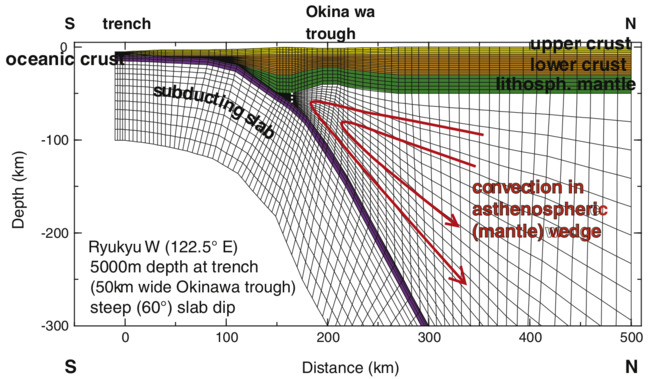
\includegraphics[width=7cm]{images/meshes/gukt16}\\
\end{center}


\Literature: \cite{jole97}

%...................................................
\subsubsection{Delaunay triangulation and Voronoi cells, and triangle-based meshes}

The topic of Delaunay\footnote{The triangulation is named after 
Boris Delaunay for his work on this topic from 1934.}
 triangulation is vast, but a simple definition can be written 
as follows:
"a Delaunay triangulation for a set P 
of points in a plane is a triangulation DT(P) such that no point in P is  
inside the circumcircle of any triangle in DT(P)." [wikipedia]
Other properties of such triangulations are that they 
maximize the minimum angle of all the angles of the 
triangles in the triangulation.
Note that for four or more 
points on the same circle (e.g., the vertices of a rectangle) the Delaunay triangulation is  
not unique and that points on a line also cannot yield a valid triangulation
(for the simple reason that they do not form a triangle).

\begin{center}
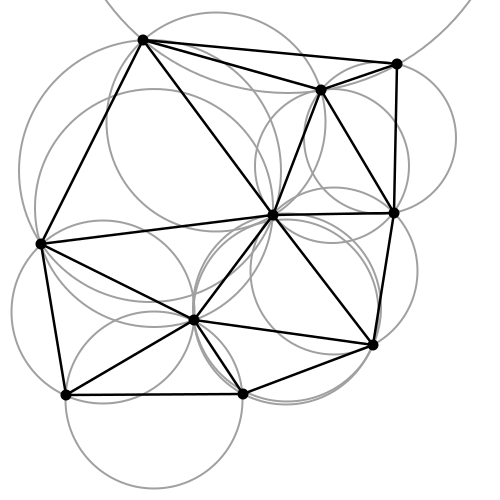
\includegraphics[width=4cm]{images/meshes/delaunay}

\includegraphics[width=4cm]{images/meshes/delaunay3}\\
{\captionfont a) A Delaunay triangulation in the plane with circumcircles shown.
b) The Delaunay triangulation of a random set of 100 points in a plane.}
\end{center}

The Delaunay triangulation of a discrete point set P in general corresponds 
to the dual graph of the Voronoi diagram for P. 
A Voronoi diagram is composed of non-overlapping Voronoi cells which make a partition 
of the plane. 
For each point there is a corresponding region consisting of all points closer to that 
point than to any other: this region is the Voronoi cell of that point.

\begin{center}
a)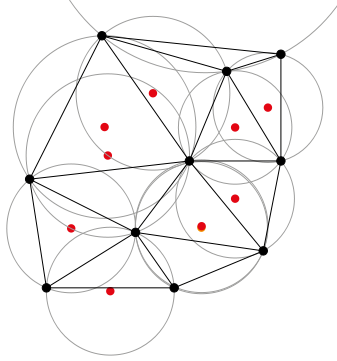
\includegraphics[width=4cm]{images/meshes/delaunay2}
b)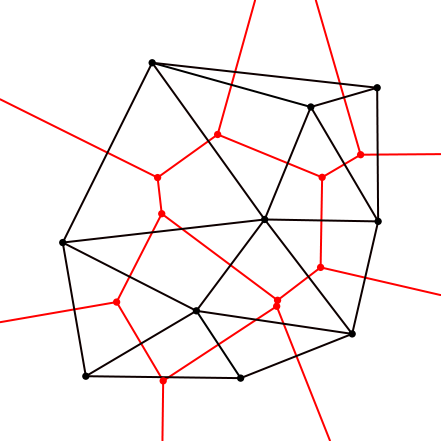
\includegraphics[width=4cm]{images/meshes/voronoi}\\
{\captionfont a) The Delaunay triangulation with all the circumcircles and their centers (in red).
b) Connecting the centers of the circumcircles produces the Voronoi diagram (in red). }
\end{center}

The Delaunay triangulation is used in the \douar code which is based on a particle levelset function to track materials. These particles are connected by means of a Delaunay triangulation (usually in a plane at startup, and then in a local Euclidean geometry once the surface is deformed) \cite{brtf08}.

\Literature: \cite{gebo}.


Once a Delaunay triangulation has been obtained it can be used as a FEM mesh.  
Triangle-based meshes are obviously better suited for simulations of complex geometries:
\begin{center}
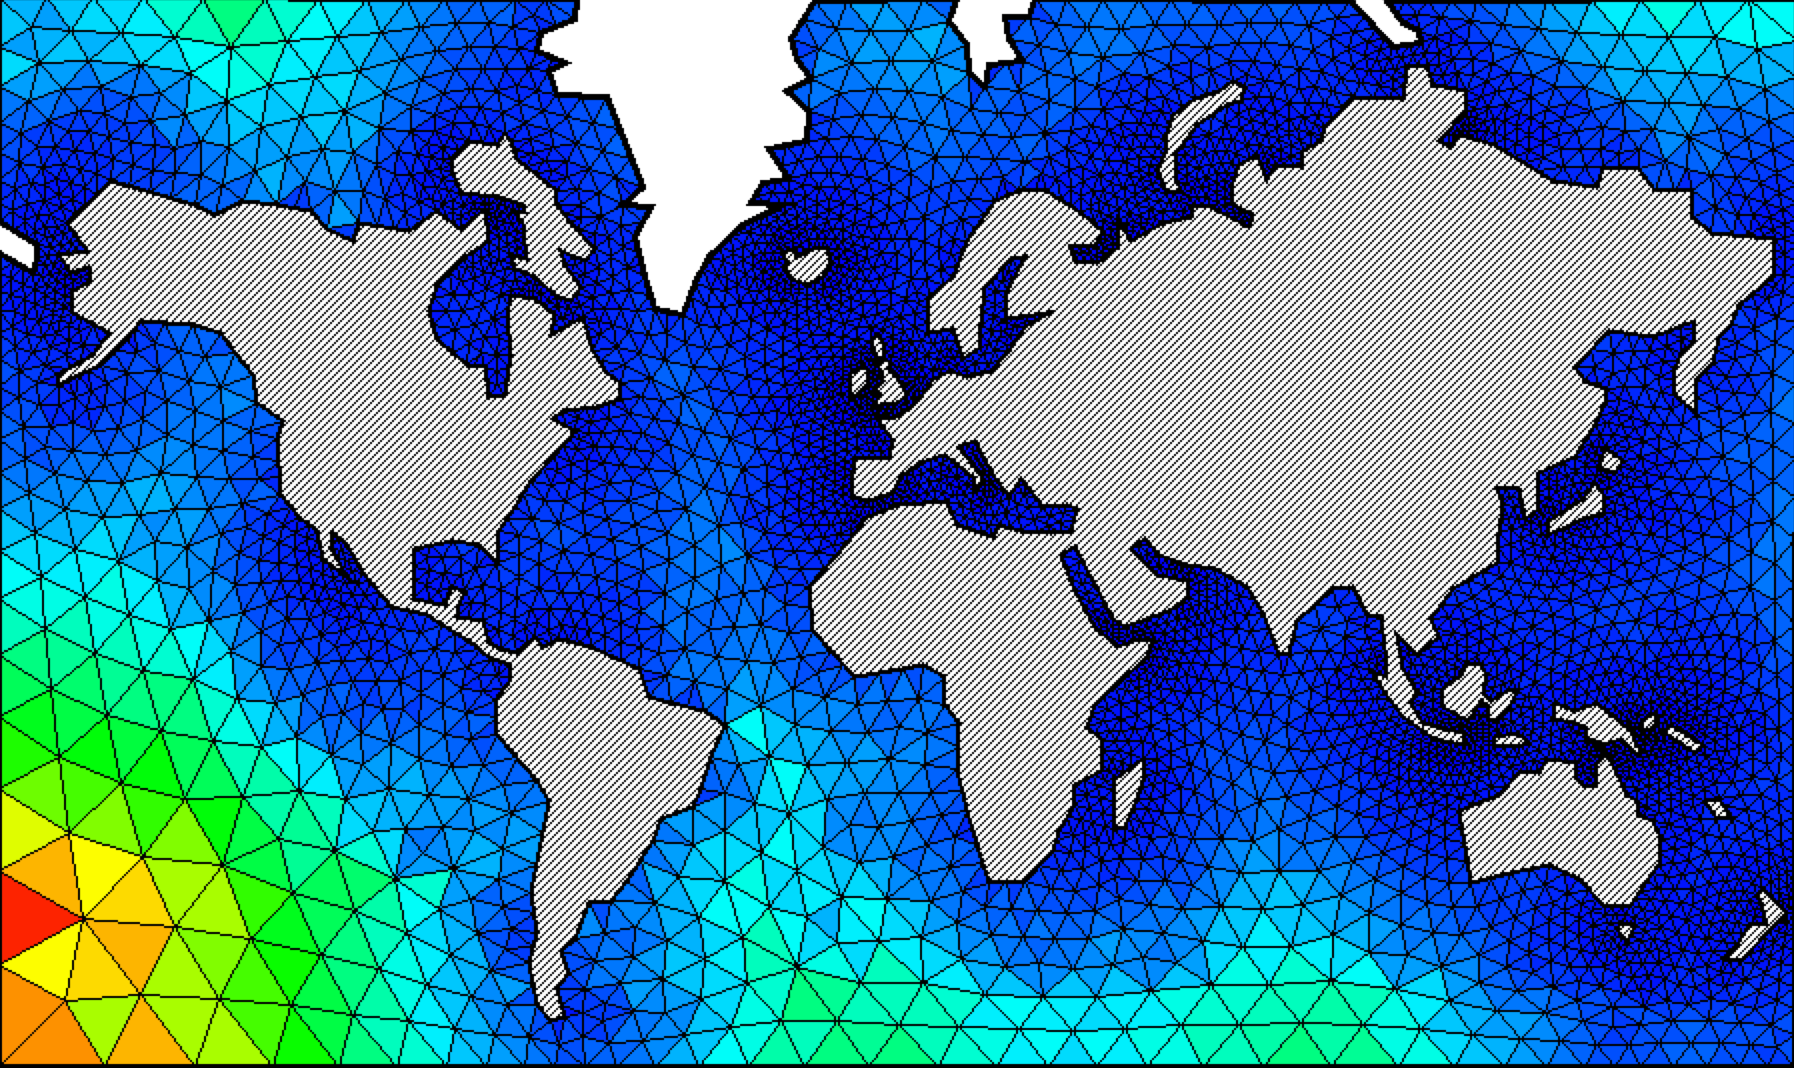
\includegraphics[height=4cm]{images/meshes/tr1}
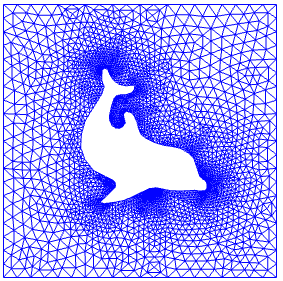
\includegraphics[height=4cm]{images/meshes/dolfin}\\
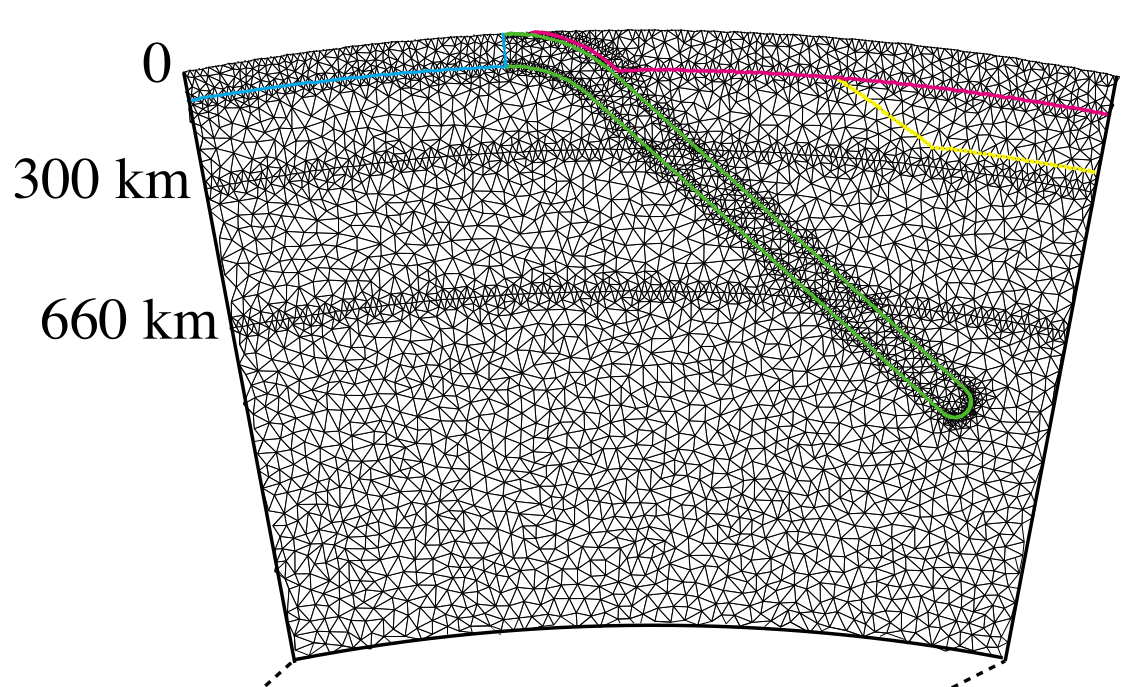
\includegraphics[height=3.8cm]{images/meshes/gebk12}\cite{gebk12}
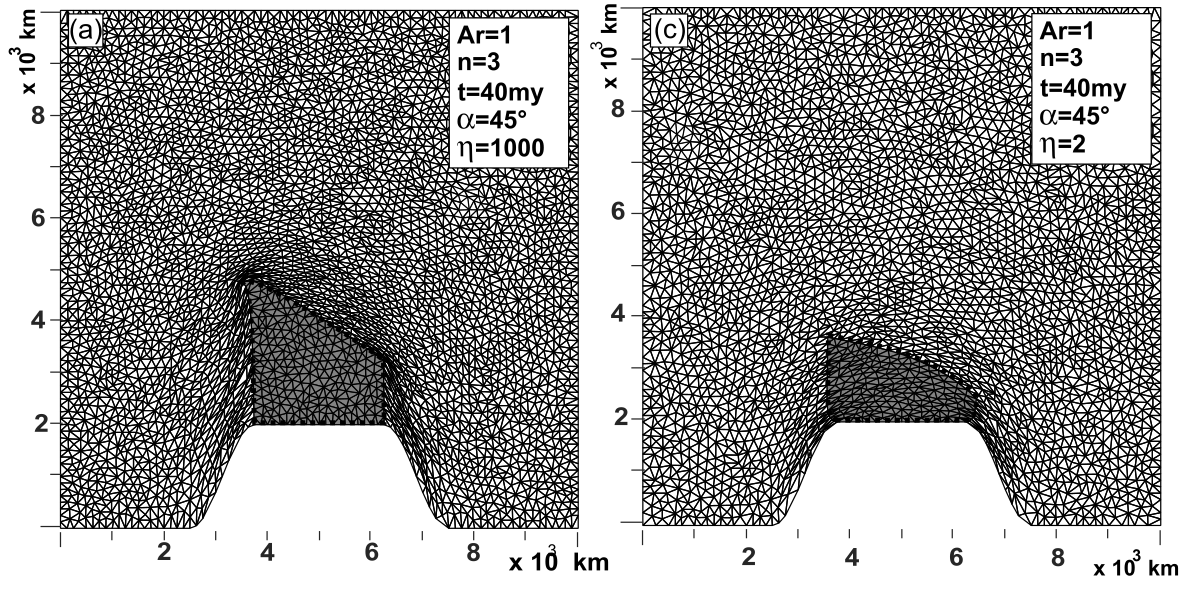
\includegraphics[height=3.8cm]{images/meshes/rost05a}\cite{rost05a}
\end{center}

A very practical 2D triangle mesher is the 
code {\sl Triangle}\footnote{\url{https://www.cs.cmu.edu/~quake/triangle.html}}
written by J.R. Shewchuk \cite{shew96,shew02,shew14}.
Triangle is specialized for creating two-dimensional finite element meshes, but can 
also perform simpler related tasks such as forming Delaunay triangulations under various assumptions.
Another very common mesher tool is Gmsh \cite{gere09}.

\begin{center}
\includegraphics[width=13cm]{images/meshes/bugw01}\\
{\captionfont Taken from Buiter \etal \cite{bugw01}. Finite element grid. 
The subducting plate initially extends to 1226 km in the horizontal direction and 
is not completely shown here. Discretization in the subducting plate is slightly coarser 
towards the right edge.}
\end{center}

\begin{center}
\includegraphics[width=13cm]{images/meshes/bafl16}\\
{\captionfont Numerical model setup of the 2D axisymmetric half-space with all applied 
boundary conditions to study the effects of ice-cap unloading
on shallow volcanic systems \cite{bafl16}}
\end{center}

\begin{center}
\includegraphics[width=13cm]{images/meshes/fegh14}\\
{\captionfont Taken from \cite{fegh14}. Modelling of slow
landslides. Finite element mesh in the initial and excavated configuration.}
\end{center}

Although it is rarely used in practice it is possible to produce meshes which contain 
both quadrilateral and triangular elements:
\begin{center}
\includegraphics[width=13cm]{images/meshes/fige95}\\
{\captionfont Mesh used to analayse the stress distribution around a pressurized crack in a layered 
elastic medium \cite{fige95}}
\end{center}

\Literature \fullcite{musd15}\fullcite{vemm09}

\begin{remark} 
The Natural Neighbour Interpolation method of Sambridge \etal \cite{sabm95,sabm96} is based on the Delaunay triangulation.
\end{remark}

\begin{remark} 
Moresi \& Mather \cite{moma19} have released Stripy, a A Python module for (constrained) triangulation
in Cartesian coordinates and on a sphere, which is based on Stripack \cite{renk96,renk97}.
\end{remark}

\todo[inline]{write about gmesh}

\begin{center}
\includegraphics[width=6cm]{images/meshes/gusa98a}
\includegraphics[width=6cm]{images/meshes/gusa98b}\\
{\captionfont Taken from Gudmundsson \& Sambridge (1998) \cite{gusa98}.
Boundaries of Voronoi cells around 4100 of the original 16,200 2x2 degree cells
selected to sample the details of the regionalization.}
\end{center}


%...........................
\subsubsection{Tetrahedra}

\begin{center}
\includegraphics[width=5cm]{images/meshes/glacier}
\includegraphics[width=10cm]{images/meshes/gowo05}\\
{\captionfont Left: Example of 3D mesh \cite{yash15}.
Right: Normalized velocities of a STEP subduction model \cite{gowo05}.}
\end{center}


\begin{center}
\includegraphics[width=7cm]{images/meshes/guyr16}
\includegraphics[width=8cm]{images/meshes/tokv09}\\
{\captionfont Left: 3D finite element grid in Damintun area, including prescribed faults. Guo \etal, 2016 \cite{guyr16}.
Right: Structural reactivation in plate tectonics controlled by olivine crystal anisotropy \cite{tokv09}.}
\end{center}



\begin{center}
\includegraphics[width=6cm]{images/meshes/paml14b}
\includegraphics[width=6.3cm]{images/meshes/codh08}\\
{\captionfont Left: Mesh used for the three-dimensional model. A high resolution mesh is used in
the wedge and subslab domains, while the mesh resolution decays to lower values
toward the edge of the model. All elements are quadratic, allowing for twice the
resolution visualized here. Paczkowski \etal (2014) \cite{paml14b}.
Right: Mid-Ocean Ridge Hydrothermal System: 3D mesh consisting of 2.5m tetrahedron elements. 
Resolution is refined toward the axial center, with the finest resolution between the dashed
lines, and colors indicate computational domains assigned to separate processors.
Coumou \etal (2008) \cite{codh08}.}
\end{center}

Check TetGen mesher \fullcite{si15}. 

%............................................
\subsubsection{Hexahedra}

A hexahedron is a convex polytope isomorphic to the cube $[0,1]^3$.
Edges are line segments, facets are strictly {\bf planar} convex polygons.

\begin{center}
\includegraphics[width=5cm]{images/meshes/hexa.jpg}
\includegraphics[width=6cm]{images/meshes/hexa2}
\end{center}

\Literature Efficient Volume computation for Three- Dimensional hexahedral Cells \cite{duko88,gran97}

%.......................................
\subsubsection{Adaptive Mesh Refinement}
\index{general}{AMR} \index{general}{Adaptive Mesh Refinement}

Let us do a simple calculation and assume we wish to model mantle convection on Earth. 
The inner radius is $R_1=$3485km and the bottom of the lithosphere is at $R_2=$6250km. 
The volume of fluid is then 
\[
V = \frac{4}{3}\pi (R_2^3-R_1^3) \simeq 8.5\times 10^{11} \text{km}^3
\]
Let us further assume that we are satisfied with an average resolution of 10km. 
Each element/cell is then $10^3\text{km}^3$ and the total number of elements/cell is then 
\[
N \simeq 8.5 \times 10^8 \sim {\cal O}(10^9)
\]
This is a very large number. The resulting linear systems from the discretisation of the 
equations on such a mesh will be very even larger for the Stokes equations and solving 
these systems will require very large numbers of CPUs and long compute times. 

Aside from these considerations it is quite obvious that a high resolution mesh is not needed 
in parts of the mantle where large scale upwellings and downwellings occur, but 
probably even higher resolution will be needed in the vicinity of thin plumes and boundary layers. 
This means that a uniform mesh is a sub-optimal way of discretising space for such problems. 

The same reasoning also holds in the lithosphere where for instance narrow plate boundaries need to 
be adequately resolved while the inside of rigid plates can be modelled with coarser meshes. 

Finally, although one could employ meshing software to arrive at well balanced meshes in space, the 
dynamic character of the geodynamics modelling renders this approach cumbersome. A subduction zone, 
a mid-ocean rift or an ascending plume will evolve in time and the mesh will have to evolve in time too. 

In light of all this, it was only a matter of time before Adaptive Mesh Refinement was adopted 
in computatinal geodynamics. However, since the use and update of such meshes is somewhat 
complex in terms of numerical algorithms, its introduction came somewhat late (00's and later).
The \douar code (see Section~\ref{app:codes}) developed originally by J. Braun and Ph. Fullsack 
is a prime example of an early multi-purpose code relying on a self-written Octree library \cite{brtf08}.
More recently the \aspect{} code was developed on top of the Octree library p4est \cite{buwg11}

For further reading I suggest you read the review by May, Schellart \& Moresi on this topic \cite{masm13}.

\begin{center}
\includegraphics[height=6cm]{images/meshes/bugg08.jpg}
\includegraphics[height=6cm]{images/meshes/bugg10.jpg}\\
{\captionfont Taken from \cite{bugg08} and \cite{bugg10}}
\end{center}

\begin{center}
\includegraphics[height=3.8cm]{images/meshes/gltf18.jpg}\\
{\captionfont Taken from \cite{gltf18}}
\end{center}


\Literature: \cite{bugg08,bugg10}\cite{lezh11} \cite[sect 3]{bugs09} \cite{dadh07}
\cite{svna18} \cite{mish11}


\newpage
\paragraph{A short illustrative exercise}.


\noindent 
\includegraphics[width=4.5cm]{images/meshes/AMR/amr0}
\includegraphics[width=4.5cm]{images/meshes/AMR/amr1}
\includegraphics[width=4.5cm]{images/meshes/AMR/amr2}\\
\includegraphics[width=4.5cm]{images/meshes/AMR/amr3}
\includegraphics[width=4.5cm]{images/meshes/AMR/amr4}
\includegraphics[width=4.5cm]{images/meshes/AMR/amr5}\\
\includegraphics[width=4.5cm]{images/meshes/AMR/amr6}
\includegraphics[width=4.5cm]{images/meshes/AMR/amr7}
\includegraphics[width=4.5cm]{images/meshes/AMR/amr8}

\begin{tabular}{l|ccccccccc}
             & \# l0  & \# l1 & \# l2 & \# l3 & \# l4 & \# l5 & \# l6 & \# l7 & \# l8 \\ 
\hline\hline
max level= 0 & 1 & \\
max level= 1 & 0 & 4 & \\
max level= 2 & 0 & 3 & 4 \\
max level= 3 & 0 & 2 & 7 & 4\\
max level= 4 & 0 & 2 & 5 & 10 & 8 \\
max level= 5 & 0 & 1 & 8 & 12 & 11 & 20 \\ 
max level= 6 & 0 & 1 & 8 & 11 & 13 & 20 & 32 \\
max level= 7 & 0 & 0 & 11 & 14 & 15 & 23 & 37 & 60 \\
max level= 8 & 0 & 0 & 11 & 13 & 17 & 27 & 43 & 72 & 116 \\
\hline
\end{tabular}

\includegraphics[width=7.28cm]{images/meshes/AMR/amr_data1.pdf}
\includegraphics[width=7.28cm]{images/meshes/AMR/amr_data2.pdf}

In the particular case presented here, even though the inclusion in a short 
two-dimensional line, the total number of elements grows faster than the 
third power of the refinement level. While of course the total number 
of elements remains much smaller than the constant resolution counterpart, 
this observation tells us that authorising a unit increase of the maximum 
refinement level can have a substantial effect on the total number of elements.

\newpage

\noindent
\includegraphics[width=4cm]{images/meshes/AMR/amr_0}
\includegraphics[width=4cm]{images/meshes/AMR/amr_1}
\includegraphics[width=4cm]{images/meshes/AMR/amr_2}
\includegraphics[width=4cm]{images/meshes/AMR/amr_3}\\
\includegraphics[width=4cm]{images/meshes/AMR/amr_4}
\includegraphics[width=4cm]{images/meshes/AMR/amr_5}
\includegraphics[width=4cm]{images/meshes/AMR/amr_6}
\includegraphics[width=4cm]{images/meshes/AMR/amr_7}


\includegraphics[width=5cm]{images/meshes/AMR/amr_data3.pdf}
\includegraphics[width=5cm]{images/meshes/AMR/amr_data4.pdf}
\includegraphics[width=5cm]{images/meshes/AMR/amr_data5.pdf}






%.......................................
\subsubsection{Conformal Mesh Refinement \label{ss:cmr}}
\index{general}{Conformal Mesh Refinement}

The quadtree/octree mesh refinement presented above is one option
when it comes to mesh refinement (or $h$-refinement). However their 
massive drawback is the presence of hanging notes which require 
special attention. 
Another approach to mesh refinement is conformal mesh refinement
as best exemplified on the following figures: 

\begin{center}
\includegraphics[height=4.5cm]{images/meshes/amrnew}\\
{\captionfont Taken from Deb \etal (1996) \cite{depl96}.
A typical instance of the outcome of the refinement procedure. 
Notice that the `spill-over' is reduced to one row on each side of the `localized' elements.}
\end{center}

\begin{center}
\includegraphics[height=4.5cm]{images/meshes/vaks15}
\includegraphics[height=4.5cm]{images/meshes/depl96}
\includegraphics[height=4.5cm]{images/meshes/habo04}\\
\includegraphics[height=4.5cm]{images/meshes/kott05}
\includegraphics[height=4.5cm]{images/meshes/specfem}\\
\includegraphics[height=4.5cm]{images/meshes/conf3D}\\
{\captionfont 
Top row, From left to right: 
van Driel \etal (2015) \cite{vaks15}; 
Deb \etal (1996) \cite{depl96}; 
Harris \etal (2004) \cite{habo04}; 
Komatitsch \etal (2005) \cite{kott05}; 
Middle row: Specfem manual;
Bottom row: I don't know anymore.}
\end{center}

\begin{center}
\includegraphics[height=5cm]{images/meshes/gari09_a}
\includegraphics[height=5cm]{images/meshes/gari09_b}\\
{\captionfont Taken from Garimella (2009) \cite{gari09}.}
\end{center}

\begin{center}
\includegraphics[height=4cm]{images/meshes/newmeshref1}
\includegraphics[height=4cm]{images/meshes/newmeshref2}
\end{center}


\begin{center}
\includegraphics[height=4cm]{images/meshes/refine_mesh_sheet_directional1}
\includegraphics[height=4cm]{images/meshes/refine_mesh_sheet_directional2}
\includegraphics[height=4cm]{images/meshes/refine_mesh_sheet_directional4}\\
\url{https://cubit.sandia.gov/public/14.0/help_manual/WebHelp/mesh_generation/mesh_modification/mesh_refinement.htm}
\end{center}

\Literature: 
D{\"u}ster \& Rank \cite{dura01},
Harris \etal (2004) \cite{habo04},
Anderson \etal (2009) \cite{anbo09},
Anderson \cite{ande09}, 
Garimella (2009) \cite{gari09},
Nicolas \& Fouquet (2013) \cite{nifo13,nifo13b}.
Parrish \cite{parr07}, 
Schneiders \cite{schn00,schn96,schn96b,schn99},
Schneiders \etal \cite{scde95},
Staten \& Canann \cite{stca97},
book by Ramm \etal \cite{rarr03}.


%.......................................
\subsubsection{Stretching the mesh}

In some cases the topology of the mesh can be regular but one can for instance stretch 
the mesh such that (for instance) the vertical resolution is higher at the top than at the bottom, 
or higher in the middle than on the sides.

The idea behind the transformation is a piecewise-linear function which maps [0,L] to [0,L] where 
$L$ is the length of the domain in the $x$-direction. For instance, this transformation can take the following form:

\begin{center}
\includegraphics[width=8cm]{images/meshes/stretching/stretch_towards_center}\\
{\captionfont Parameters $\beta_1$ and $\beta_2$ control the shape of the lines.\\ 
The kinks in the line occur at $\beta_1 L$ and $(1-\beta_1)L$ (see code here under).}
\end{center}

The (minimal) code to transform the mesh is as follows:
\begin{lstlisting}
def stretch_towards_center(x,L,beta1,beta2):
    if x<beta1*L: 
       val = beta2/beta1*x
    elif x<(1.-beta1)*L: 
       val = (1-2*beta2)/(1-2*beta1)*(x-beta1*L)+beta2*L
    else:
       val=beta2/beta1*(x-(1-beta1)*L)+(1-beta2)*L
    return val

[...]

beta1=0.25
beta2=0.375

for i in range(0,NV):
    x[i]=stretch_towards_center(x[i],Lx,beta1,beta2)
\end{lstlisting}

The following meshes count 64x16 elements. The top one is a regular mesh, with square elements, 
while the second one has been stretched by means of the transformation above:

\begin{center}
\includegraphics[width=8cm]{images/meshes/stretching/stretch_x}
\end{center}

Concerning the stretching towards the top of the model domain, the transformation line is as follows:

\begin{center}
\includegraphics[width=8cm]{images/meshes/stretching/stretch_towards_top}\\
{\captionfont Parameters $\beta_1$ and $\beta_2$ control the shape of the lines. The kinks in the 
line occur at $\beta_1 L$ and $(1-\beta_1)L$.\\ The slope of the left line is $\beta_2/\beta_1 x$.}
\end{center}

The (minimal) code to transform the mesh is as follows:
\begin{lstlisting}
def stretch_towards_top(x,L,beta1,beta2):
    if x<beta1*L: 
       val=beta2/beta1*x
    else:
       val=(1-beta2)/(1-beta1)*(x-beta1*L)+beta2*L
    return val

[...]

beta1=0.25
beta2=0.5
for i in range(0,NV):
    y[i]=stretch_towards_top(y[i],Ly,beta1,beta2)
\end{lstlisting}


The following meshes count 64x16 elements. The top one is a regular mesh, with square elements, 
while the second one has been stretched by means of the transformation above.
\begin{center}
\includegraphics[width=8cm]{images/meshes/stretching/stretch_y}
\end{center}

Finally both transformations can be applied to the same mesh:
\begin{center}
\includegraphics[width=8cm]{images/meshes/stretching/stretch_xy}
\end{center}

This approach is used in \stone 67.

%.......................................
\subsubsection{Meshes in an annulus}


\begin{center}
\includegraphics[width=6.8cm]{images/meshes/brhv08}
\includegraphics[width=6.8cm]{images/meshes/brva07a}\\
{\captionfont The quadratic finite element mesh as used in 
Brandenburg \etal \cite{brhv08,brva07a}}
\end{center}


%.......................................
\subsubsection{Meshes in a hollow sphere}

The following is for the most part published in Thieulot (2018) \cite{thie18}.

To a first approximation the Earth is a sphere: the Earth's polar diameter is 
about 43 kilometers shorter than its equatorial diameter, a negligible difference of 
about 0.3\%. As a consequence, modelling physical processes 
which take place in the planet require the discretisation of a sphere. 
Furthermore, because core dynamics occur on vastly difference time scales than mantle dynamics, mantle 
modelling usually leaves the core out, thereby requiring simulations to be run on a hollow sphere mesh
(with the noticeable exception of \cite{geyu07}).

Although so-called latitude-longitude grids would seem appealing, 
they suffer from the convergence of meridians at the poles
(resulting in over sampling at poles) and the juxtaposition of triangles 
near the poles and quadrilaterals elsewhere. 
As a consequence more regular, but more complex, grids have been designed 
over the years which tesselate the surface of the 
sphere into triangles or quadrilaterals (sometimes overlapping).
There is the 'cubed sphere' \cite{roip96,heta03,chob05,sthh06,chcc07,brmw10,yiym19},
the Yin-Yang grid \cite{kasa04,yoka04,yoka06,kaks08,tack08,crta14,crta16},
the Yin-Yang-zhong grid \cite{haka16}, the Yin-yang grid of 
Shahnas \& Peltier \cite{shpe15}, the spiral grid \cite{hust08}, 
an icosahedron-based grid \cite{bafr85,tasu01},
or a grid composed of 12 blocks further subdivided into quadrilaterals \cite{zhzm00} 
as used in the CitcomS code.
Note that \cite{oldp12} have also presented a method for generating a numerical 
grid on a spherical surface which 
allows the grid to be based on several different regular polyhedrons (including octahedron, 
cube, icosahedron, and rhombic dodecahedron). 
Ideally, one wishes to generate a mesh that is regular,
i.e. angles between edges/faces as close to $90^\circ$ as possible, 
of approximately similar volumes.


\begin{center}
\includegraphics[width=12cm]{images/meshes/kaks08}\\
{\captionfont Example of Yin-Yang grid. Taken from Kameyama \etal (2008) \cite{kaks08}.}
\end{center}

How such meshes are built is often not discussed in the literature. It is 
a tedious exercise of three-dimensional geometry and it can be time-consuming, especially 
the connectivity array generation. In Thieulot (2018) \cite{thie18} I present an open source 
mesh generator for three hollow sphere meshes: the 'cubed sphere' mesh, the CitcomS mesh and the 
icosahedral mesh:

\begin{itemize}
\item 
The cubed sphere ('HS06'), composed of 6 blocks which 
are themselves subdivided into $N_b \times N_b$ quadrilateral shaped cells  \cite{sado72,roip96,heta03,busa13}.
Four types of cubed spheres meshes have been proposed: the conformal, elliptic, gnomonic and spring types \cite{puli07}:


\begin{center}
\includegraphics[width=6.5cm]{images/meshes/puli07}
\includegraphics[width=8.5cm]{images/meshes/cubed_nair}\\
{\captionfont 
Left: The cubed-sphere grids at $2^\circ$ resolution displaying cells on the sphere,
 the image focuses on the distribution of grid cells near one corner of the grid;
 (a) conformal mapping \cite{rapm96,mcgr96}, (b) the gnomonic grid modified by elliptic solver,
 (c) equiangular gnomonic mapping and (d) the gnomonic grid modified by spring dynamics. \cite{puli07}.
Right: Taken from presentation by R. Nair, see Nair2008.pdf
}
\end{center}

However only gnomonic meshes are considered in Thieulot (2018): these 
are obtained by inscribing a cube within a sphere and expanding to the surface
of the sphere.
The cubed sphere has been used in large-scale mantle convection simulation in conjunction with 
Adaptive Mesh Refinement \cite{algs12,busa13}.  

\begin{center}
\includegraphics[width=4cm]{images/ghost/hs06}
\end{center}



\item 
The CitcomS mesh ('HS12') composed of 12 blocks also subdivided 
into $N_b \times N_b$ quadrilateral shaped cells
\cite{zhzm00,sthh06,zhmt08,arfw14}.
Note that \aspect{} \cite{krhb12,hedg17}, a relatively new code aimed at 
superseeding CitcomS can generate and use 
this type of mesh \cite{thie17} but is not limited to it.

\begin{center}
\includegraphics[width=4cm]{images/ghost/citcom12}
\end{center}


\item The icosahedral mesh ('HS20') composed of 20 triangular blocks \cite{bafr85,baum85} subdivided into triangles, which is 
used in the TERRA code \cite{burb96,burb97,burl98,dadb13}.
\end{itemize}


\begin{center}
\includegraphics[width=8cm]{images/meshes/spherical_choices1}
\includegraphics[width=8cm]{images/meshes/spherical_choices2}\\
{\captionfont source?}
\end{center}



Given the regularity and symmetry of these meshes determining the location of the 
mesh nodes in space is a relatively straightforward task. Building the mesh connectivity in an 
efficient manner is where the difficulty lies.

The approach to building all three meshes is identical:
\begin{enumerate}
\item A reference square or triangle is populated with cells,
parametrised by a level $l$: the square is subdivided into $l\times l$ quadrilaterals while 
the triangle is subdivided into $l^2$ triangles.
\begin{center}
\includegraphics[width=8cm]{images/ghost/f01_basics}\\
{\captionfont Reference square and triangles meshes at level 5.}
\end{center}

\item This reference square or triangle is then replicated {\sl nblock} times (6, 12 or 20) and mapped
onto a portion of a unit sphere. The blocks are such that their union covers a full sphere
but they cannot overlap except at the edges:
\begin{center}
\includegraphics[width=.8\linewidth]{images/ghost/f02}\\
{\captionfont From left to right: HS06, HS12 and HS20 shells coloured by block number.}
\end{center}

\item All block meshes are then merged together to generate a shell mesh. This task is rather 
complex as duplicate nodes must be removed and all connectivity arrays of the blocks must then 
be mended accordingly. 

\item Shell meshes are replicated {\sl nlayer+1} times outwards with increasing radii. 
The {\sl nlayer} shells are then merged together to form a hollow sphere mesh:
\begin{center}
\includegraphics[width=10cm]{images/ghost/f03_3HS}\\
{\captionfont a) HS06 mesh composed of 6 blocks containing each $6^3$ cells; 
b) HS12 mesh composed of 12 blocks containing each 
$6^3$ cells; e) HS20 mesh composed of 20 blocks containing each $6^3$ cells.}
\end{center}

\end{enumerate}



More information on these steps is available in the manual of the code.
In the following table the number of nodes and cells for a variety of resolutions 
for all three mesh types is reported. Looking at the CitcomS literature of the past 20 years, we find that 
the mesh data presented in this table cover the various resolutions used, e.g.
$12\times48^3$ \cite{mczh04,arfw14}, $12\times64^3$ \cite{budt14}
$12\times96^3$ \cite{bumb10}, $12\times128^3$ \cite{beck06,wele16,welm16}.
Note that in the case of the HS06 and HS12 meshes the mesh nodes are mapped out to the 6 or 12 blocks 
following either an equidistant or equiangle approach (see \cite{puli07}
for details on both approaches). 

\begin{center}
\begin{tabular}{lrrrl}
\hline
type & level & $N$ & $N_{el}$ & structure\\
\hline
\hline
HS06 & 
2   &  78        &  48         &$6\times 2^3$    \\
HS06 & 
4   &  490       &  384        &$6\times 4^3$    \\
HS06 & 
8   &  3,474      &  3,072       &$6\times 8^3$    \\
HS06 & 
16  &  26,146     &  24,576      &$6\times 16^3$    \\
HS06 & 
32  &  202,818    &  196,608     &$6\times 32^3$    \\
HS06 & 
64  &  1,597,570   &  1,572,864    &$6\times 64^3$    \\
HS06 & 
128 &  12,681,474  &  12,582,912   &$6\times 128^3$    \\
HS06 & 
256 &  101,057,026 &  100,663,296  &$6\times 256^3$    \\
\hline
HS12 & 2    &          150  &          96  &  $12\times 2^3$ \\
HS12 & 4    &          970  &         768  &  $12\times 4^3$ \\
HS12 & 8    &        6,930  &       6,144  &  $12\times 8^3$ \\
HS12 & 16   &       52,258  &      49,152  &  $12\times 16^3$ \\
HS12 & 32   &      405,570  &     393,216  &  $12\times 32^3$ \\
HS12 & 48   &    1,354,850  &   1,327,104  &  $12\times 48^3$ \\
HS12 & 64   &    3,195,010  &   3,145,728  &  $12\times 64^3$ \\
HS12 & 128  &   25,362,690  &  25,165,824  &  $12\times 128^3$ \\
HS12 & 256  &  202,113,538  & 201,326,592  &  $12\times 256^3$ \\
\hline
HS20 & 
2     &         126  &         160   & $20 \times 2^3$ \\
HS20 & 
4     &         810  &       1,280   & $20 \times 4^3$ \\
HS20 & 
8     &       5,778  &      10,240   & $20 \times 8^3$ \\
HS20 & 
16    &      43,554  &      81,920   & $20 \times 16^3$ \\
HS20 & 
32    &     337,986  &     655,360   & $20 \times 32^3$ \\
HS20 & 
64    &   2,662,530  &   5,242,880   & $20 \times 64^3$ \\
HS20 & 
128   &  21,135,618  &  41,943,040   & $20 \times 128^3$ \\
HS20 & 
256   & 168,428,034  & 335,544,320   & $20 \times 256^3$ \\
\hline
\end{tabular}\\
{\captionfont Number of nodes $N$ and elements/cells $N_{el}$ for the three types of meshes and for various 
levels.\\ HS06: cubed sphere; HS12: CitcomS mesh; HS20: icosahedral mesh.}
\end{center}

There are also many possibilities offered by the use of tetrahedral cells/elements:


\begin{center}
\includegraphics[width=7cm]{images/meshes/oebm09}\\
{\captionfont Grid of a global neo-tectonic SHELLS model coupled to a global mantle
circulation model; colours represent temperatures (red=hot, blue=cold)
at a depth of $200\si{km}$ below the surface. Taken from Oeser \etal (2009) \cite{oebm09}.}
\end{center}


\begin{center}
\includegraphics[width=7cm]{images/meshes/htm}\\
{\captionfont Example of a Hierarchical Triangular Mesh}
\end{center}


\begin{center}
\includegraphics[width=7cm]{images/meshes/bafr85}
\includegraphics[width=7cm]{images/meshes/simj12}\\
{\captionfont \cite{bafr85}, \cite{simj12}}
\end{center}


\Literature: Phillips \etal \cite{phdo19} present an algorithm which builds polyhedral-based grids.





 %--------

\newpage %---------------------------------------------------------------------
\subsection{Visco-Plasticity} 
\Literature: \cite{mumc03,chpe15,momu06,muso11}





















IMPLEMENTATION of plasticity ... WORK IN PROGRESS

%%%%%%%%%%%%%%%%%%%%%%%%%%%%%%%%%%%%%%%%%%%%%%%%%%%%%%%%%%%%%%%%%%%%%%%%%%%%%%%%%%%%%%%%%%%%%%%%%%%%
\subsubsection{Scalar viscoplasticity}

This formulation is quite easy to implement. It is widely used, e.g. \cite{will92,thfb08,spmw16}, and relies on the assumption that 
a scalar quantity $\eta_p$ (the 'effective plastic viscosity') exists such that the deviatoric stress tensor 
\begin{equation}
{\bm \tau}=2\eta_p \dot{\bm\varepsilon} \label{eqscpl1}
\end{equation}
is bounded by some yield stress value $Y$.
From Eq. (\ref{eqscpl1}) it follows that ${\tau}_{e}= 2\eta_p \dot{\varepsilon}_{e}=Y$ which yields
\begin{mdframed}[backgroundcolor=blue!5]
\[
\eta_p = \frac{Y}{2 \dot{\varepsilon}_{e}}
\]
\end{mdframed}
This approach has also been coined the Viscosity Rescaling Method (VRM) \cite{kacha04}. 
\index{general}{VRM} \index{general}{Viscosity Rescaling Method}

\improvement[inline]{insert here the rederivation 2.1.1 of spmw16}

It is at this stage important to realise that (i) in areas where the strainrate is low, the resulting effective viscosity will be large, and 
(ii) in areas where the strainrate is high, the resulting effective viscosity will be low. This is not without consequences since 
(effective) viscosity contrasts up to 8-10 orders of magnitude have been observed/obtained with this formulation and it makes the FE 
matrix very stiff, leading to (iterative) solver convergence issues.
In order to contain these viscosity contrasts one usually resorts to viscosity limiters $\eta_{min}$ and $\eta_{max}$ such that 
\[
\eta_{min} \leq \eta_p \leq \eta_{max}
\]
Caution must be taken when choosing both values as they may influence the final results.


%-------------------------------------------------
{Work in progress}

\Literature \cite{zico74,zigo74,zico74b,zien75,corm75,zigo75,zihl75,zijo78,vidm82,vidm84,vede84,zivt85,vimd86}
\cite{wasd97,debo88,debo01,hesd02,bewv11,mumg10,leor89,sccm13,desm93,demu92,debo91,shmv16}
\cite{modm01}\cite{baji02}\cite{slde92}\cite{lepo13}
\cite{modm02}\cite{vavd99}\cite{miam13}\cite{huly99}\cite{hugh83}

Note that \cite{vidm82,vidm84,vimd86,zivt85} use the following formulation which they attribute to \cite{zijo78}:
\[
\eta_{eff} = \frac{c + (\dot{\varepsilon}_e / \gamma)^{1/n}}{ \dot{\varepsilon}_e }
\] 
For a perfectly plastic flow law, $\gamma \rightarrow \infty$ and then 
\[
\eta_{eff} = \frac{c}{ \dot{\varepsilon}_e }
\] 
and when when $c=0$ then the effective viscosity is essentially of the power law type.
Also, when $n=1$ the formulation becomes identical to the v-vp formulation (when the max viscosity is infinite) and with $1/\gamma=\eta_{min}$.

fractal distribution of shear bands in \cite{pohp94}



 %------------------------

\newpage %---------------------------------------------------------------------
\subsection{Pressure smoothing} 
It has been widely documented that the use of the $Q_1 \times P_0$ element is 
not without problems. Aside from the 
consequences it has on the FE matrix properties, we will here focus on another unavoidable side effect: 
the spurious pressure checkerboard modes. 
\index{general}{Pressure Smoothing} 
\index{general}{Checkerboard mode}

These modes have been thoroughly analysed decades ago, see for instance
Hughes et al (1979)\cite{hulb79}, 
Sani et al (1981) \cite{sagl81a,sagl81b},
Griffiths \& Silvester (1994) \cite{grsi94}.
They can be filtered out(Chen (1995)  \cite{chpc95}) 
or simply smoothed (Lee et al (1979) \cite{legs79}), as we will see later.
Nodes on edges and corners may need special treatment as documented in Sani et al \cite{sagl81a} or
Lee et al (1979) \cite{legs79}.
The list of 8 schemes is not exhaustive with regards to the above mentioned publications. 
There has been considerable amount of work on the topic and this section is 
unfortunately not representing the literature appropriately.

\mscthesis: Get all relevant literature, digest it, implement all variants in fieldstone 12.
 \index{general}{MSc Thesis} 


On the following figure (a,b), pressure fields for the lid driven cavity experiment 
are presented for both an even and un-even number of elements. We see that 
the amplitude of the modes can sometimes be so large that the 'real' pressure signal is 
not visible under the checkerboard and that something as simple as the number of elements in the 
domain can trigger those or not at all.

\begin{center}
a)\includegraphics[width=4cm]{images/checkerboard/p_el}
\includegraphics[width=4cm]{images/checkerboard/p_el_33x33}
b)\includegraphics[width=5cm]{images/checkerboard/press_doneahuerta}
c)\includegraphics[width=7cm]{images/checkerboard/douarpunch}\\
{\captionfont a) element pressure for a 32x32 grid and for a 33x33 grid;\\ 
b) image from \cite[p307]{dohu03} for a manufactured solution;
c) elemental pressure and smoothed pressure for the punch experiment \cite{thfb08}}
\end{center}

%----------------------------------------------------------------------
\paragraph{Scheme 1}.

The easiest post-processing step that can be used (especially when a regular grid is used) 
is explained in Thieulot et al (2008) \cite{thfb08}: "The element-to-node interpolation is performed by
averaging the elemental values from elements common to each node; 
the node-to-element interpolation is performed
by averaging the nodal values element-by-element. This
method is not only very efficient but produces a smoothing
of the pressure that is adapted to the local density of the
octree. Note that these two steps can be repeated until a
satisfying level of smoothness (and diffusion) of the pressure field is attained."


\begin{center}
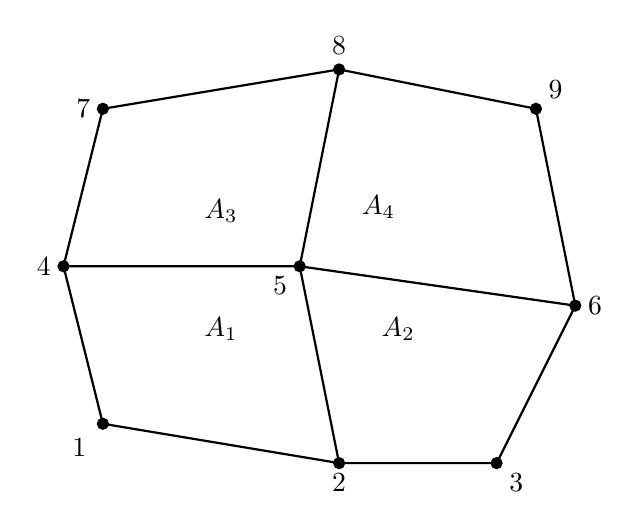
\begin{tikzpicture}
%\draw[fill=gray!5,gray!5](0,0) rectangle (9,7);
%\draw[step=0.5cm,gray,very thin] (0,0) grid (9,7); %background grid
\draw[thick](1.5,1.5) -- (4.5,1) -- (6.5,1) -- (7.5,3) -- (7,5.5) -- (4.5,6) --(1.5,5.5) -- (1,3.5) -- cycle;  
\draw[thick](4.5,1)--(4,3.5)--(4.5,6);
\draw[thick](1,3.5)--(4,3.5)--(7.5,3);
\draw[black,fill=black] (1.5,1.5) circle (2pt); \node[] at (1.2,1.2){1}; %1
\draw[black,fill=black] (4.5,1)   circle (2pt); \node[] at (4.5,0.75){2}; %2
\draw[black,fill=black] (6.5,1)   circle (2pt); \node[] at (6.75,0.75){3}; %3
\draw[black,fill=black] (1,3.5)   circle (2pt); \node[] at (0.75,3.5){4}; %4
\draw[black,fill=black] (4,3.5)   circle (2pt); \node[] at (3.75,3.25){5}; %5
\draw[black,fill=black] (7.5,3)   circle (2pt); \node[] at (7.75,3){6}; %6
\draw[black,fill=black] (1.5,5.5) circle (2pt); \node[] at (1.25,5.5){7}; %7
\draw[black,fill=black] (4.5,6)   circle (2pt); \node[] at (4.5,6.3){8}; %8
\draw[black,fill=black] (7,5.5)   circle (2pt); \node[] at (7.25,5.75){9}; %9
%\draw[thin,dashed](1,3.5)--(4.5,1)--(7.5,3)--(4.5,6)--cycle;
\node[] at (3,2.7){$A_1$}; %8
\node[] at (5.25,2.7){$A_2$}; %8
\node[] at (5,4.25){$A_4$}; %8
\node[] at (3,4.2){$A_3$}; %8
\end{tikzpicture}
\end{center}
\[
q_5^{(1)} = \frac{1}{4}\sum_{e=1}^4 p_e
\] 

In the codes which rely on the $Q_1 \times P_0$ element, the (elemental) pressure
is simply defined as 
\begin{lstlisting}
p=np.zeros(nel,dtype=np.float64)  
\end{lstlisting}
while the nodal pressure is then defined as\footnote{In virtually all stones $p$
stands for the 'raw' pressure and $q$ stands for its projection onto the velocity mesh.} 
\begin{lstlisting}
q=np.zeros(nnp,dtype=np.float64)  
\end{lstlisting}
The element-to-node algorithm is then simply (in 2D):

\begin{lstlisting}
count=np.zeros(nnp,dtype=np.int32)  
for iel in range(0,nel):
    q[icon[0,iel]]+=p[iel]
    q[icon[1,iel]]+=p[iel]
    q[icon[2,iel]]+=p[iel]
    q[icon[3,iel]]+=p[iel]
    count[icon[0,iel]]+=1
    count[icon[1,iel]]+=1
    count[icon[2,iel]]+=1
    count[icon[3,iel]]+=1
q=q/count
\end{lstlisting}



%----------------------------------------------------------------------
\paragraph{Schemes 2,3}.

{\sl Schemes 2,3} are very similar and are presented in Sani et al (1981) \cite{sagl81a,sagl81b}.
Scheme 2 uses the areas of the surrounding elements as weights for the arithmetic averaging
while scheme 3 uses the area of the triangles:

\begin{multicols}{2}

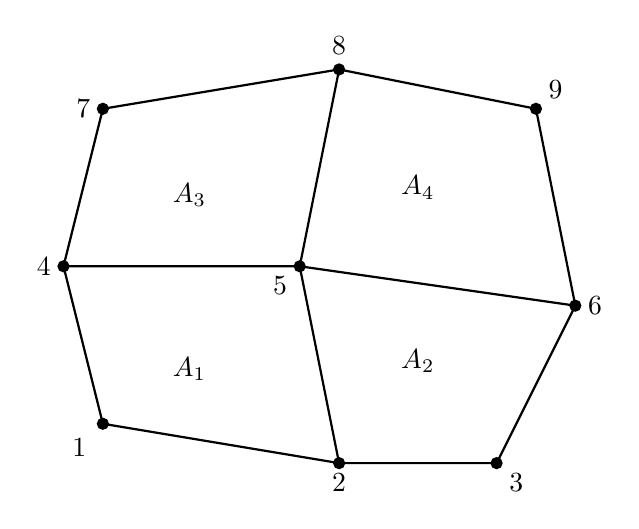
\begin{tikzpicture}
%\draw[fill=gray!5,gray!5](0,0) rectangle (9,7);
%\draw[step=0.5cm,gray,very thin] (0,0) grid (9,7); %background grid
\draw[thick](1.5,1.5) -- (4.5,1) -- (6.5,1) -- (7.5,3) -- (7,5.5) -- (4.5,6) --(1.5,5.5) -- (1,3.5) -- cycle;  
\draw[thick](4.5,1)--(4,3.5)--(4.5,6);
\draw[thick](1,3.5)--(4,3.5)--(7.5,3);
\draw[black,fill=black] (1.5,1.5) circle (2pt); \node[] at (1.2,1.2){1}; %1
\draw[black,fill=black] (4.5,1)   circle (2pt); \node[] at (4.5,0.75){2}; %2
\draw[black,fill=black] (6.5,1)   circle (2pt); \node[] at (6.75,0.75){3}; %3
\draw[black,fill=black] (1,3.5)   circle (2pt); \node[] at (0.75,3.5){4}; %4
\draw[black,fill=black] (4,3.5)   circle (2pt); \node[] at (3.75,3.25){5}; %5
\draw[black,fill=black] (7.5,3)   circle (2pt); \node[] at (7.75,3){6}; %6
\draw[black,fill=black] (1.5,5.5) circle (2pt); \node[] at (1.25,5.5){7}; %7
\draw[black,fill=black] (4.5,6)   circle (2pt); \node[] at (4.5,6.3){8}; %8
\draw[black,fill=black] (7,5.5)   circle (2pt); \node[] at (7.25,5.75){9}; %9
\node[] at (2.6,2.2){$A_1$}; %8
\node[] at (5.5,2.3){$A_2$}; %8
\node[] at (2.6,4.4){$A_3$}; %8
\node[] at (5.5,4.5){$A_4$}; %8
\end{tikzpicture}

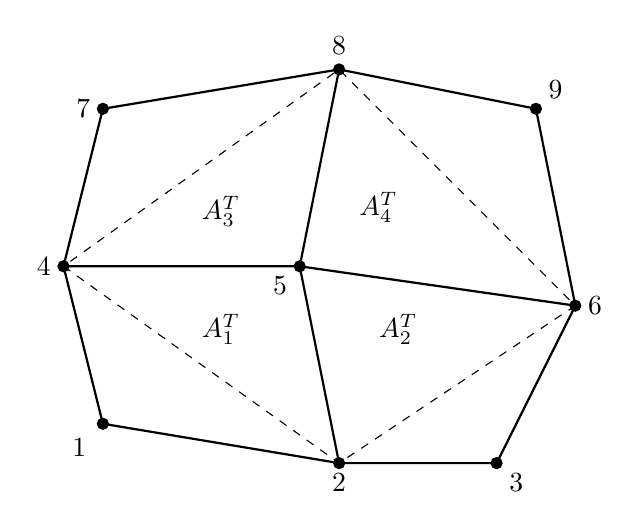
\begin{tikzpicture}
%\draw[fill=gray!5,gray!5](0,0) rectangle (9,7);
%\draw[step=0.5cm,gray,very thin] (0,0) grid (9,7); %background grid
\draw[thick](1.5,1.5) -- (4.5,1) -- (6.5,1) -- (7.5,3) -- (7,5.5) -- (4.5,6) --(1.5,5.5) -- (1,3.5) -- cycle;  
\draw[thick](4.5,1)--(4,3.5)--(4.5,6);
\draw[thick](1,3.5)--(4,3.5)--(7.5,3);
\draw[black,fill=black] (1.5,1.5) circle (2pt); \node[] at (1.2,1.2){1}; %1
\draw[black,fill=black] (4.5,1)   circle (2pt); \node[] at (4.5,0.75){2}; %2
\draw[black,fill=black] (6.5,1)   circle (2pt); \node[] at (6.75,0.75){3}; %3
\draw[black,fill=black] (1,3.5)   circle (2pt); \node[] at (0.75,3.5){4}; %4
\draw[black,fill=black] (4,3.5)   circle (2pt); \node[] at (3.75,3.25){5}; %5
\draw[black,fill=black] (7.5,3)   circle (2pt); \node[] at (7.75,3){6}; %6
\draw[black,fill=black] (1.5,5.5) circle (2pt); \node[] at (1.25,5.5){7}; %7
\draw[black,fill=black] (4.5,6)   circle (2pt); \node[] at (4.5,6.3){8}; %8
\draw[black,fill=black] (7,5.5)   circle (2pt); \node[] at (7.25,5.75){9}; %9
\draw[thin,dashed](1,3.5)--(4.5,1)--(7.5,3)--(4.5,6)--cycle;
\node[] at (3,2.7){$A_1^T$}; %8
\node[] at (5.25,2.7){$A_2^T$}; %8
\node[] at (5,4.25){$A_4^T$}; %8
\node[] at (3,4.2){$A_3^T$}; %8
\end{tikzpicture}

\end{multicols}




\[
q_5^{(2)} = \frac{\sum\limits_{e=1}^4 A_e p_e}{\sum\limits_{e=1}^4 A_e}
\qquad
\qquad
q_5^{(3)} = \frac{\sum\limits_{e=1}^4 A_e^T p_e}{\sum\limits_{e=1}^4 A_e^T}
\] 


\begin{remark} Although Schemes 1,2,3 are similar, scheme 1 is the simplest and fastest
to implement since the areas of neighbouring elements/triangles are not needed.
\end{remark}

\begin{remark} 
Schemes 1,2,3 are identical if all elements are rectangles of identical dimensions.
\end{remark}




%----------------------------------------------------------------------
\paragraph{Scheme 4} This scheme has been designed by me. 
It resembles the last three ones, but the weighing is in this case different.

Let us consider a 1D problem:
\begin{center}
\includegraphics[width=0.5\linewidth]{images/pressure_smoothing/newalgo.png}
\end{center}

Elemental pressures $p_1$ and $p_2$ corresponding to elements 1 and 2 respectively are known at
locations $x_1$ and $x_2$. The two elements have a different size, characterised in this case
by the distances $d_1$ and $d_2$ to their common edge.

The equation of the line passing through points $(x_1,p_1)$ and $(x_2,p_2)$ is 
\[
p(x)=\frac{p_2-p_1}{x_2-x_1}(x-x_1)+p_1
\]
The $x$ coordinate of the common edge is given by $x=x_1+d_1/2$, 
and since $x_2-x_1=(d_1+d_2)/2$, the 
pressure at this location writes:
\[
p(x_M)= \frac{p_2-p_1}{d_1+d_2}d_1+p_1 = \frac{\frac{p_1}{d_1} + \frac{p_2}{d_2}}{\frac{1}{d_1} + \frac{1}{d_2}}
\]
Extrapolating this formula to 2D, $d_1$ and $d_2$ are in fact the element volumes, so that
\[
q_5^{(4)} = 
\frac{\sum\limits_{j=1}^4 \frac{p_j^e}{A_j^e}}{\sum\limits_{j=1}^4 \frac{1}{A_j^e}}
=
\frac{
\frac{p_1^e}{A_1^e}+
\frac{p_2^e}{A_2^e}+
\frac{p_3^e}{A_3^e}+
\frac{p_4^e}{A_4^e}
}{
\frac{1}{A_1^e}+
\frac{1}{A_2^e}+
\frac{1}{A_3^e}+
\frac{1}{A_4^e}
}\]

There remains a problem, due to the presence of the boundary nodes for which 
the sums present in the above equation do not run up to 4. A boundary
node only has three neighbours and a corner node only two. Additional measures
are required for these nodes. 

\begin{center}
\includegraphics[width=0.5\linewidth]{images/pressure_smoothing/newalgo_corner.png}
\end{center}

The pressure value $p_N$ is obtained as follows:
\[
q_N = \frac{ 
 \frac{p_2^e}   {A_2^e}
+\frac{p_3^e}   {A_3^e}
+\frac{p_{2'}^e}{A_{2'}^e}
+\frac{p_{3'}^e}{A_{3'}^e}
}{
 \frac{1}{A_2^e}
+\frac{1}{A_3^e}
+\frac{1}{A_{2'}^e}
+\frac{1}{A_{3'}^e}
}
\]
The areas and pressures of the mirrored elements 2' and 3' are extrapolated from the areas of elements 2 and 6, and 3 and 7 respectively. 
Likewise the pressure $p_M$ at the corner node is obtained through the pressures of its surrounding elements.


%------------------------------------------------------------------------------
\paragraph{Scheme 5 - Least squares} This scheme is presented (among other places) in Lee et al (1979)
\cite{legs79}. 
Let us start from the patch of 4 $Q_1$ elements counting 9 nodes: 

\begin{center}
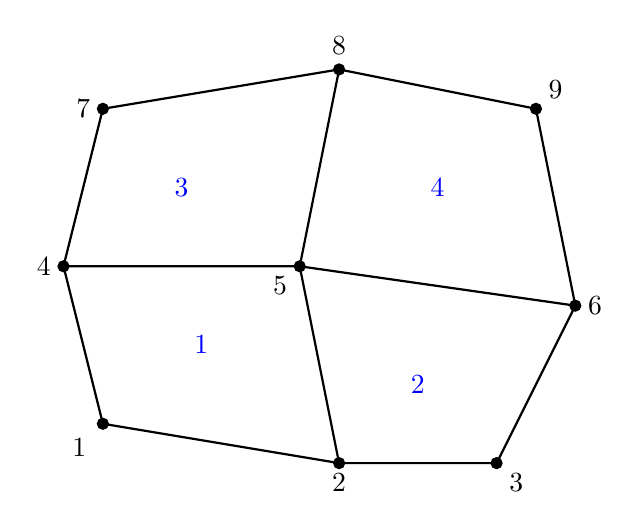
\begin{tikzpicture}
%\draw[fill=gray!5,gray!5](0,0) rectangle (9,7);
%\draw[step=0.5cm,gray,very thin] (0,0) grid (9,7); %background grid
\draw[thick](1.5,1.5) -- (4.5,1) -- (6.5,1) -- (7.5,3) -- (7,5.5) -- (4.5,6) --(1.5,5.5) -- (1,3.5) -- cycle;  
\draw[thick](4.5,1)--(4,3.5)--(4.5,6);
\draw[thick](1,3.5)--(4,3.5)--(7.5,3);

\node[] at (2.75,2.5) {\color{blue}1};
\node[] at (5.5,2) {\color{blue}2};
\node[] at (2.5,4.5) {\color{blue}3};
\node[] at (5.75,4.5) {\color{blue}4};

\draw[black,fill=black] (1.5,1.5) circle (2pt); \node[] at (1.2,1.2){1}; %1
\draw[black,fill=black] (4.5,1)   circle (2pt); \node[] at (4.5,0.75){2}; %2
\draw[black,fill=black] (6.5,1)   circle (2pt); \node[] at (6.75,0.75){3}; %3
\draw[black,fill=black] (1,3.5)   circle (2pt); \node[] at (0.75,3.5){4}; %4
\draw[black,fill=black] (4,3.5)   circle (2pt); \node[] at (3.75,3.25){5}; %5
\draw[black,fill=black] (7.5,3)   circle (2pt); \node[] at (7.75,3){6}; %6
\draw[black,fill=black] (1.5,5.5) circle (2pt); \node[] at (1.25,5.5){7}; %7
\draw[black,fill=black] (4.5,6)   circle (2pt); \node[] at (4.5,6.3){8}; %8
\draw[black,fill=black] (7,5.5)   circle (2pt); \node[] at (7.25,5.75){9}; %9

\end{tikzpicture}
\end{center}



We are looking for a field $q$ living on the nodes.
We build the quantity
\[
J=\iint_\Omega (q-p)^2 dV
\]
where $p$ is the elemental field. To make things clearer we split the integral into 
the sum of elemental integrals:
\[
J=
\iint_{\Omega_1} (q(x,y)-p_1)^2 dV+
\iint_{\Omega_2} (q(x,y)-p_2)^2 dV+
\iint_{\Omega_3} (q(x,y)-p_3)^2 dV+
\iint_{\Omega_4} (q(x,y)-p_4)^2 dV
\]
Inside each element the field $q(x,y)$ is given by a bilinear interpolation so that:
\begin{eqnarray}
J
&=& \iint_{\Omega_1} (N_1(x,y) q_1 + N_2(x,y)q_2 + N_5(x,y)q_5 + N_4(x,y)q_4 -p_1)^2 dV \nn\\
&+& \iint_{\Omega_2} (N_2(x,y) q_2 + N_3(x,y)q_3 + N_6(x,y)q_6 + N_5(x,y)q_5 -p_2)^2 dV \nn\\
&+& \iint_{\Omega_3} (N_4(x,y) q_4 + N_5(x,y)q_5 + N_8(x,y)q_8 + N_7(x,y)q_7 -p_3)^2 dV \nn\\
&+& \iint_{\Omega_4} (N_5(x,y) q_5 + N_6(x,y)q_6 + N_9(x,y)q_9 + N_8(x,y)q_8 -p_4)^2 dV 
\end{eqnarray}
where the $N_i$ functions are the shape functions (unusually expressed in $x,y$ coordinates).
The least square procedure looks for the set of $q_i$ such that 
\[
\frac{\partial J}{\partial q_i} =0 \qquad \forall i=1,...9
\]
and this yields 9 equations/constraints for 9 unknowns.
\begin{eqnarray}
\frac{\partial J}{\partial q_1} 
&=& \iint_{\Omega_1} 2 (N_1(x,y) q_1 + N_2(x,y)q_2 + N_5(x,y)q_5 + N_4(x,y)q_4 -p_1) N_1(x,y) dV \nn\\
\frac{\partial J}{\partial q_2}
&=& \iint_{\Omega_1} 2(N_1(x,y) q_1 + N_2(x,y)q_2 + N_5(x,y)q_5 + N_4(x,y)q_4 -p_1) N_2(x,y) dV \nn\\
&+& \iint_{\Omega_2} 2(N_2(x,y) q_2 + N_3(x,y)q_3 + N_6(x,y)q_6 + N_5(x,y)q_5 -p_2) N_2(x,y) dV \nn\\
\frac{\partial J}{\partial q_3}
&=& \iint_{\Omega_2} 2(N_2(x,y) q_2 + N_3(x,y)q_3 + N_6(x,y)q_6 + N_5(x,y)q_5 -p_2) N_3(x,y) dV \nn\\
\frac{\partial J}{\partial q_4}
&=& \iint_{\Omega_1} 2(N_1(x,y) q_1 + N_2(x,y)q_2 + N_5(x,y)q_5 + N_4(x,y)q_4 -p_1) N_4(x,y) dV \nn\\
&+& \iint_{\Omega_3} 2(N_4(x,y) q_4 + N_5(x,y)q_5 + N_8(x,y)q_8 + N_7(x,y)q_7 -p_3) N_4(x,y) dV \nn\\
\frac{\partial J}{\partial q_5}
&=& \iint_{\Omega_1} 2(N_1(x,y) q_1 + N_2(x,y)q_2 + N_5(x,y)q_5 + N_4(x,y)q_4 -p_1) N_5(x,y) dV \nn\\
&+& \iint_{\Omega_2} 2(N_2(x,y) q_2 + N_3(x,y)q_3 + N_6(x,y)q_6 + N_5(x,y)q_5 -p_2) N_5(x,y) dV \nn\\
&+& \iint_{\Omega_3} 2(N_4(x,y) q_4 + N_5(x,y)q_5 + N_8(x,y)q_8 + N_7(x,y)q_7 -p_3) N_5(x,y) dV \nn\\
&+& \iint_{\Omega_4} 2(N_5(x,y) q_5 + N_6(x,y)q_6 + N_9(x,y)q_9 + N_8(x,y)q_8 -p_4) N_5(x,y) dV \nn\\
\frac{\partial J}{\partial q_6}
&=& \iint_{\Omega_2} 2(N_2(x,y) q_2 + N_3(x,y)q_3 + N_6(x,y)q_6 + N_5(x,y)q_5 -p_2) N_6(x,y) dV \nn\\
&+& \iint_{\Omega_4} 2(N_5(x,y) q_5 + N_6(x,y)q_6 + N_9(x,y)q_9 + N_8(x,y)q_8 -p_4) N_6(x,y) dV \nn\\
\frac{\partial J}{\partial q_7}
&=& \iint_{\Omega_3} 2(N_4(x,y) q_4 + N_5(x,y)q_5 + N_8(x,y)q_8 + N_7(x,y)q_7 -p_3) N_7(x,y) dV \nn\\
\frac{\partial J}{\partial q_8}
&=& \iint_{\Omega_3} 2(N_4(x,y) q_4 + N_5(x,y)q_5 + N_8(x,y)q_8 + N_7(x,y)q_7 -p_3) N_8(x,y)dV \nn\\
&+& \iint_{\Omega_4} 2(N_5(x,y) q_5 + N_6(x,y)q_6 + N_9(x,y)q_9 + N_8(x,y)q_8 -p_4) N_8(x,y)dV \nn\\ 
\frac{\partial J}{\partial q_9}
&=& \iint_{\Omega_4} 2(N_5(x,y) q_5 + N_6(x,y)q_6 + N_9(x,y)q_9 + N_8(x,y)q_8 -p_4) N_9(x,y)dV 
\end{eqnarray}
The factor 2 are removed and the terms $\int p_i N_j $ are known so they end up in the right hand side.

\begin{eqnarray}
 \iint_{\Omega_1} (N_1N_1 q_1 + N_1N_2 q_2 + N_1N_5q_5 + N_1N_4q_4) dV &=& \iint_{\Omega_1} p_1 N_1 dV \nn\\
 \iint_{\Omega_1} (N_2 N_1  q_1 + N_2 N_2q_2 + N_2 N_5q_5 + N_2 N_4q_4)  dV \nn\\
+\iint_{\Omega_2} (N_2 N_2 q_2 + N_3 N_2 q_3 + N_6 N_2 q_6 + N_5 N_2 q_5) dV 
&=& \iint_{\Omega_1} p_1N_2 dV + \iint_{\Omega_2}  p_2 N_2 dV \nn\\
\nn\\
\dots &=& \dots \nn\\
\nn\\
 \iint_{\Omega_4} (N_9N_5 q_5 + N_9N_6q_6 + N_9N_9q_9 + N_9N_8q_8) dV &=&  \iint_{\Omega_4} p_4 N_9 dV 
\end{eqnarray}

The mass matrices corresponding to the four elements are 
\[
{\bm M}_1 = \int_{\Omega_1} \left( \begin{array}{cccc}
N_1 N_1 & N_1 N_2 & N_1 N_5 & N_1 N_4 \\
N_2 N_1 & N_2 N_2 & N_2 N_5 & N_2 N_4 \\
N_5 N_1 & N_5 N_2 & N_5 N_5 & N_5 N_4 \\
N_4 N_1 & N_4 N_2 & N_4 N_5 & N_4 N_4 
\end{array}\right) dV
\qquad
{\bm M}_2 = \int_{\Omega_2} \left( \begin{array}{cccc}
N_2 N_2 & N_2 N_3 & N_2 N_6 & N_2 N_5 \\
N_3 N_2 & N_3 N_3 & N_3 N_6 & N_3 N_5 \\
N_6 N_2 & N_6 N_3 & N_6 N_6 & N_6 N_5 \\
N_5 N_2 & N_5 N_3 & N_5 N_6 & N_5 N_5 
\end{array}\right) dV
\]
\[
{\bm M}_3 = \int_{\Omega_3} \left( \begin{array}{cccc}
N_4 N_4 & N_4 N_5 & N_4 N_8 & N_4 N_7 \\
N_5 N_4 & N_5 N_5 & N_5 N_8 & N_5 N_7 \\
N_8 N_4 & N_8 N_5 & N_8 N_8 & N_8 N_7 \\
N_7 N_4 & N_7 N_5 & N_7 N_8 & N_7 N_7 
\end{array}\right) dV
\qquad
{\bm M}_4 = \int_{\Omega_4} \left( \begin{array}{cccc}
N_5 N_5 & N_5 N_6 & N_5 N_9 & N_5 N_8 \\
N_6 N_5 & N_6 N_6 & N_6 N_9 & N_6 N_8 \\
N_9 N_5 & N_9 N_6 & N_9 N_9 & N_9 N_8 \\
N_8 N_5 & N_8 N_6 & N_8 N_9 & N_8 N_8 
\end{array}\right) dV
\]
so that the 9 equations above are actually the result of the assembly process of these four 
elemental systems:
\[
\left( \iint_{\Omega_e} \vec{N}^T\vec{N} dV \right) \cdot \vec{q}_e = \iint_{\Omega_i} \vec{N}^T p_e dV 
\qquad\qquad e=1,2,3,4
\]


%------------------------------------------------------------------------------
\paragraph{Scheme 6 - Consistent pressure recovery}

The is the method presented in Zienkiewicz \& Nakazawa (1982) \cite{zina82}. In the second part 
of this publication the authors wish to establish a simple and effective numerical method to calculate 
variables eliminated by the penalisation process. 
The method involves an additional finite element solution for the nodal pressures using 
the same finite element basis and numerical quadrature as used for the velocity.

Let us start with\footnote{I here voluntarily use $q$ instead of $p$}:
\[
q = -\lambda \vec\nabla\cdot \vec\upnu
\]
We are going to treat this equation as any other PDE in the context of the FE method, i.e. 
we are going to establish its weak form. 
We assume that the pressure is given inside an element by
\[
q(x,y) = \sum_{i=1}^4 N_i(x,y) q_i = \vec{N} \cdot \vec{q}
\]
and the velocity:
\[
\vec\upnu = (u,v) 
\qquad 
\qquad 
u(x,y)  = \sum_{i=1}^4 N_i(x,y) u_i
\qquad 
\qquad 
v(x,y)  = \sum_{i=1}^4 N_i(x,y) v_i
\]
where the $N_i$ are the $Q_1$ shape functions and $q_i$ are the sought after nodal values. 
We multiply the equation above by a $Q_1$ shape function $N_i$ and integrate over the whole domain:
\[
\iint_\Omega N_i(x,y) q(x,y) \; dxdy = -\lambda \iint_\Omega N_i \vec\nabla\cdot \vec\upnu  \; dx dy
\]
As before we now focus on the above expression inside a single element $e$:
\[
\iint_{\Omega_e} N_i(x,y) q(x,y) \; dxdy = -\lambda \iint_{\Omega_e} N_i \vec\nabla\cdot \vec\upnu \; dx dy
\]
After $N_i \rightarrow \vec{N}=(N_1,N_2,N_3,N_4)^T$, the left hand side term becomes:
\[
\iint _{\Omega_e} \vec{N}^T q(x,y) \; dxdy 
=
\iint _{\Omega_e} \vec{N}^T \vec{N} \cdot \vec{q} \; dxdy 
=
\left(\underbrace{\iint _{\Omega_e} \vec{N}^T \vec{N} dxdy}_{{\bm M}_e} \right) \cdot \vec{q}  
\]
where ${\bm M}_e$ is the elemental mass matrix.
We now turn to the right hand side. We have
\[
\vec\nabla\cdot \vec\upnu
= \frac{\partial u}{\partial x}+\frac{\partial v}{\partial y}
= \sum_i \frac{\partial N_i}{\partial x} u_i + \sum_i \frac{\partial N_i}{\partial y} v_i 
\]
We here too define $\vec{V}_e=(u_1,v_1,u_2,v_2,u_3,v_3,u_4,v_4)^T$ so that 

\begin{eqnarray}
&& \iint_{\Omega_e} \vec{N} {\vec \nabla}\cdot {\vec \upnu} \; d\Omega \nn\\
&=& \iint_{\Omega_e} \vec{N}^T \sum_{i=1}^{4} 
\left( \frac{\partial N_i}{\partial x} u_i + \frac{\partial N_i}{\partial y} v_i 
\right)  
d\Omega \nonumber\\
&=& 
\iint_{\Omega_e} 
\left(
\begin{array}{c}
N_1 \left(
\sum\limits_{i=1}^{4} \frac{\partial N_i}{\partial x} u_i +
\sum\limits_{i=1}^{4} \frac{\partial N_i}{\partial y} v_i \right) \\
N_2 \left(
\sum\limits_{i=1}^{4} \frac{\partial N_i}{\partial x} u_i +
\sum\limits_{i=1}^{4} \frac{\partial N_i}{\partial y} v_i \right) \\
N_3 \left(
\sum\limits_{i=1}^{4} \frac{\partial N_i}{\partial x} u_i +
\sum\limits_{i=1}^{4} \frac{\partial N_i}{\partial y} v_i \right) \\
N_4 \left(
\sum\limits_{i=1}^{4} \frac{\partial N_i}{\partial x} u_i +
\sum\limits_{i=1}^{4} \frac{\partial N_i}{\partial y} v_i \right) 
\end{array}
\right) d \Omega \nonumber \\  %%%%%%%%%%%%%%%%%%%%%%%%%%
&=& 
\int_{\Omega_e} 
\left(
\begin{array}{ccc}
{N}_1& {N}_1 &  0 \\\\
{N}_2& {N}_2 &  0 \\\\
{N}_3& {N}_3 &  0 \\\\
{N}_4& {N}_4 &  0 
\end{array}
\right)
\cdot
\left(
\begin{array}{c}
\sum\limits_i \frac{\partial N_i}{\partial x} u_i \\ \\
\sum\limits_i \frac{\partial N_i}{\partial y} v_i \\ \\
\sum\limits_i (\frac{\partial N_i}{\partial y} u_i\! +\! \frac{\partial N_i}{\partial x} v_i) 
\end{array}
\right)
\; d\Omega \nonumber\\ %%%%%%%%%%%%%%%%%%%%%%%%%%
&=& 
\int_{\Omega_e} 
\underbrace{
\left(
\begin{array}{cccccc}
{N}_1 & {N}_1 &  0 \\
{N}_2 & {N}_2 &  0 \\
{N}_3 & {N}_3 &  0 \\
{N}_4 & {N}_4 &  0 
\end{array}
\right)
}_{{\bm N}}
\cdot
\underbrace{
\left(\begin{array}{cccccccc}
\partial_x N_1 & 0 &  
\partial_x N_2 & 0 &  
\partial_x N_3 & 0 &  
\partial_x N_4 & 0 \\ \\
0 & \partial_y N_1 &   
0 & \partial_y N_2 &   
0 & \partial_y N_3 &   
0 & \partial_y N_4 \\ \\
\partial_y N_1 & \partial_x N_1 &  
\partial_y N_2 & \partial_x N_2 &  
\partial_y N_3 & \partial_x N_3 &  
\partial_y N_4 & \partial_x N_4 
\end{array}\right)}_{{\bm B}}
\cdot \vec{V}_e
\; d\Omega  \nonumber \\
&=& 
\left(\int_{\Omega_e} {\bm N} \cdot {\bm B} \; d\Omega \right) \cdot \vec{V}_e \nonumber\\
&=& -\G_e^T \cdot {\vec V}_e
\end{eqnarray}

After assembly we arrive at
\[
{\bm M} \cdot \vec{q} = \lambda \G^T \cdot {\vec V} 
\qquad
\text{with}
\qquad
\G_e = -\int_{\Omega_e} {\bm N} \cdot {\bm B} \; d\Omega
\]
where ${\bm M}$ is the global mass matrix, $\vec{q}$ the vector of all 
nodal pressures, $\G$ the discrete gradient matrix and $\vec{V}$
the (velocity) solution vector. 
The system can be easily solved since the mass matrix is a friendly matrix.
The vector ${\vec q}$ contains the nodal pressure values directly, with 
no need for a smoothing scheme! 

\begin{remark}
Very importantly, the mass matrix ${\bm M}$ is to be evaluated at the full integration points, 
while the constraint part (the right hand side of the equation) is to be evaluated at 
the reduced integration point, i.e. in the middle of the element.  
\end{remark}

\begin{remark}
As noted in \cite{zina82}, it is interesting to note that when linear elements are used 
and the lumped matrices are used for the ${\bm M}$ the resulting algebraic equation is identical 
to the smoothing scheme 1 only if a uniform square finite element 
mesh is used. In this respect this method is expected to yield different results when elements 
are not square or even rectangular.
\end{remark}

\begin{remark}
The third column of the matrix ${\bm N}$
and the last line of the ${\bm B}$ matrix could be removed altogether.
If your code is based on the mixed formulation, then you already 
have built matrix $\G$ so you can easily re-use this piece of code 
to compute $\G$ again, this time with a reduced integration quadrature.
If you are using the penalty formulation then you need to program 
all from scratch and then simply do away with these unnecessary terms, or 
you can direcly build the rhs as $\int_{\Omega_e} \vec{N}^T p_e$ (assuming
you have previously computed the pressure in the middle of each element 
by means of $p=-\lambda\vec\nabla\cdot\vec\upnu$).
\end{remark}

\begin{remark}
This  scheme is identical to the least square scheme!
\end{remark}


%--------------------------------------------------------------
\paragraph{Scheme 7}

Same as scheme 6, but with lumped mass matrix.  


%--------------------------------------------------------------
\paragraph{Scheme 8 - bilinear interpolation} Let us assume that the centers of the 
four elements make a $Q_1$ quadrilateral element, as shown on this figure:


\begin{center}
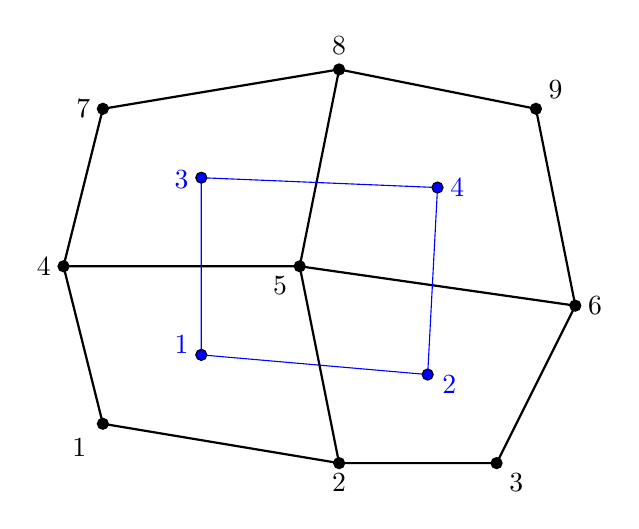
\begin{tikzpicture}
%\draw[fill=gray!5,gray!5](0,0) rectangle (9,7);
%\draw[step=0.5cm,gray,very thin] (0,0) grid (9,7); %background grid
\draw[thick](1.5,1.5) -- (4.5,1) -- (6.5,1) -- (7.5,3) -- (7,5.5) -- (4.5,6) --(1.5,5.5) -- (1,3.5) -- cycle;  
\draw[thick](4.5,1)--(4,3.5)--(4.5,6);
\draw[thick](1,3.5)--(4,3.5)--(7.5,3);

\draw[black,fill=blue] (2.75,2.375) circle (2pt); 
\node[] at (2.5,2.5) {\color{blue}1};
\draw[black,fill=blue] (5.625,2.125) circle (2pt); 
\node[] at (5.9,2) {\color{blue}2};
\draw[black,fill=blue] (5.75,4.5) circle (2pt); 
\node[] at (2.5,4.6) {\color{blue}3};
\draw[black,fill=blue] (2.75,4.625) circle (2pt); 
\node[] at (6,4.5) {\color{blue}4};

\draw[black,fill=black] (1.5,1.5) circle (2pt); \node[] at (1.2,1.2){1}; %1
\draw[black,fill=black] (4.5,1)   circle (2pt); \node[] at (4.5,0.75){2}; %2
\draw[black,fill=black] (6.5,1)   circle (2pt); \node[] at (6.75,0.75){3}; %3
\draw[black,fill=black] (1,3.5)   circle (2pt); \node[] at (0.75,3.5){4}; %4
\draw[black,fill=black] (4,3.5)   circle (2pt); \node[] at (3.75,3.25){5}; %5
\draw[black,fill=black] (7.5,3)   circle (2pt); \node[] at (7.75,3){6}; %6
\draw[black,fill=black] (1.5,5.5) circle (2pt); \node[] at (1.25,5.5){7}; %7
\draw[black,fill=black] (4.5,6)   circle (2pt); \node[] at (4.5,6.3){8}; %8
\draw[black,fill=black] (7,5.5)   circle (2pt); \node[] at (7.25,5.75){9}; %9

\draw[blue](2.75,2.375)--(5.625,2.125)--(5.75,4.5)--(2.75,4.625)--cycle;
\end{tikzpicture}
\end{center}




The values at the corners are $p_1$,
$p_2$, $p_3$ and $p_4$. Assuming that the pressure inside this element can be represented 
by a bilinear field, we have 
\[
p(x,y)= a+ bx +cy +dxy
\]
where the coefficients will be determined by ensuring that $p(x_i,y_i)=p_i$ for $i=1,2,3,4$, or:
\begin{eqnarray}
a+bx_1+cy_1+dx_1y_1 &=& p_1 \\
a+bx_2+cy_2+dx_2y_2 &=& p_2 \\
a+bx_3+cy_3+dx_3y_3 &=& p_3 \\
a+bx_4+cy_4+dx_4y_4 &=& p_4 
\end{eqnarray}
i.e.
\[
\left(
\begin{array}{cccc}
1 & x_1 & y_1 & x_1y_1 \\
1 & x_2 & y_2 & x_2y_2 \\
1 & x_3 & y_3 & x_3y_3 \\
1 & x_4 & y_4 & x_4y_4
\end{array}
\right)\cdot
\left(
\begin{array}{c}
a \\b\\c\\d
\end{array}
\right)
=
\left(
\begin{array}{c}
p_1\\p_2\\p_3\\p_4
\end{array}
\right)
\]

There remains an issue with nodes which are on the boundaries of the domain. These are of course not 
'surrounded' by four pressure values so the above algorithm does not apply directly. However, looking 
at the above figure, and assuming that node 1 is a lower left corner of a 2D domain, we can use the 
bilinear interpolation based on elements 1,2,3,4 to extrapolate a nodal pressure value at node 1. 
The same would apply for nodes 2 and 4 for example. 

\begin{remark}
This scheme is not applicable to quadtree-based meshed.
\end{remark}




 %-------------------

\newpage %---------------------------------------------------------------------
\subsection{Pressure scaling} \index{pressure scaling}

As perfectly explained in the step 32 of deal.ii\footnote{https://www.dealii.org/9.0.0/doxygen/deal.II/step\_32.html},
we often need to scale the $\G$ term since it is many orders of magnitude smaller than $\K$, 
which introduces large inaccuracies in the solving process to the point that the solution is nonsensical. 
This scaling coefficient is $\eta/L$. 
We start from 
\[
\left(
\begin{array}{cc}
\K & \G \\ \G^T & 0 
\end{array}
\right)
\cdot
\left(
\begin{array}{c}
{\cal V} \\ {\cal P}
\end{array}
\right)
=
\left(
\begin{array}{c}
 f \\ h
\end{array}
\right)
\]
and introduce the scaling coefficient as follows (which in fact does not alter the solution at all):
\[
\left(
\begin{array}{cc}
\K & \frac{\eta}{L}\G \\ \frac{\eta}{L}\G^T & 0 
\end{array}
\right)
\cdot
\left(
\begin{array}{c}
{\cal V} \\\frac{L}{\eta} {\cal P}
\end{array}
\right)
=
\left(
\begin{array}{c}
 f \\ \frac{\eta}{L} h
\end{array}
\right)
\]
We then end up with the modified Stokes system:
\[
\left(
\begin{array}{cc}
\K & \underline{\G} \\ \underline{\G}^T & 0 
\end{array}
\right)
\cdot
\left(
\begin{array}{c}
{\cal V} \\ \underline{\cal P}
\end{array}
\right)
=
\left(
\begin{array}{c}
 f \\ \underline{h}
\end{array}
\right)
\]
where 
\[
\underline{\G}=\frac{\eta}{L}\G
\quad\quad
\quad\quad
\underline{\cal P}=\frac{L}{\eta} {\cal P}
\quad\quad
\quad\quad
\underline{h}=\frac{\eta}{L}h
\]
After the solve phase, we recover the real pressure with ${\cal P}=\frac{\eta}{L}{\cal P}'$.





 %-----------------------

\newpage %---------------------------------------------------------------------
\subsection{Pressure normalisation} 
%..................................................
\subsubsection{Basic idea and naive implementation}

When Dirichlet boundary conditions are imposed everywhere on the boundary, 
pressure is only present by its gradient in 
the equations. It is thus determined up to an arbitrary constant (one speaks then 
of a nullspace of size 1).  \index{nullspace}
In such a case, one commonly impose the average of the pressure over the whole domain or on 
a subset of the boundary 
to have a zero average, i.e.
\begin{equation}
\int_\Omega p dV = 0
\end{equation}
Another possibility is to impose the pressure value at a single node. 

Let us assume for example that we are using $Q_1 \times P_0$ elements. Then the pressure is constant 
inside each element. 
The integral above becomes:
\begin{equation}
\int_\Omega p dV = 
\sum_e  \int_{\Omega_e} p dV = 
\sum_e  p_e \int_{\Omega_e} dV = 
\sum_e  p_e A_e = 0
\end{equation}
where the sum runs over all elements $e$ of area $A_e$.
This can be rewritten 
\[
\LLL^T \cdot \vec{\cal P}=0
\] 
and it is a constraint on the pressure solution which couples {\it all} pressure dofs. 
As we have seen before \ref{XXX}, we can associate to it a 
Lagrange multiplier $\lambda$ so that we must solve the modified Stokes system:
\[
\left(
\begin{array}{ccc}
\K & \G & 0\\ 
\G^T & 0 & \LLL \\
0 & \LLL^T & 0
\end{array}
\right)
\cdot
\left(
\begin{array}{c}
\vec{\cal V} \\ \vec{\cal P} \\ \lambda
\end{array}
\right)
=
\left(
\begin{array}{c}
\vec{f} \\ \vec{h} \\ 0
\end{array}
\right)
\]
When higher order spaces are used for pressure (continuous or discontinuous)
one must then carry out the above integration numerically by means of (usually)
a Gauss-Legendre quadrature.

Although valid, this approach has one main disadvantage: it makes the Stokes matrix larger (although
marginally so -- only one row and column are added), but more importantly it prevents the use of some
of the solving strategies of Section \ref{sec:solvers}.


%..................................................
\subsubsection{Implementation -- the real deal}

The idea is actually quite simple and requires two steps:
\begin{enumerate}
\item remove the null space by prescribing the pressure at one location and solve the system;
\item post-process the pressure so as to arrive at a pressure field which fulfills the required normalisation (surface, volume, ...)
\end{enumerate}

The reason why it works is as follows: a constant pressure value lies in the null space, so that one can 
add or delete any value to the pressure field without consequence. As such I can choose said constant such that 
the pressure at a given node/element is zero. All other computed pressures are then relative to that one. 
The post-processing step will redistribute a constant value to all pressures (it will shift them up or down)
so that the normalising condition is respected. 





 %----------

\newpage %---------------------------------------------------------------------
\subsection{Convergence criterion for nonlinear iterations}


\newpage %---------------------------------------------------------------------
\subsection{The choice of solvers} 
Let us start again from the (full) Stokes system:
\begin{equation}
\left(
\begin{array}{cc}
\K & \G \\ \G^T & -\C 
\end{array}
\right)
\cdot
\left(
\begin{array}{c}
\vec{\cal V} \\ \vec{\cal P}
\end{array}
\right)
=
\left(
\begin{array}{c}
\vec{f} \\ \vec{h}
\end{array}
\right)
\label{StokesSyst}
\end{equation}
We need to solve this system in order to obtain the solution, i.e. the $\vec{\cal V}$ 
and $\vec{\cal P}$ vectors. But how? 
Unfortunately, this question is not simple to answer and the appropriate method depends on many 
parameters, but mainly on how big the matrix blocks are and what the condition number of the matrix $\K$ is. 

In what follow I cover:
\begin{itemize}
\item solving when the penalty approach is used
\item the Schur complement approach
\item the FGMRES approach \cite{deit13}
\end{itemize}

\Literature \cite{pasa75,mamo08,fumt11,knke04,kool00,kopo93} \cite{lane18}

Preconditioners \Literature: \cite{seuv10}

%...................................................
\subsubsection{When using the penalty formulation}

In this case we are only solving for 
velocity since pressure is recovered in a post-processing step:
\[
(\K_\eta+\K_\lambda) \cdot \vec {\cal V} = \vec f
\]
 We also know that 
the penalty factor $\lambda$ is many orders of magnitude higher than the viscosity and 
in combination with the use of the $Q_1 \times P_0$ element the resulting matrix 
condition number is very high so that the use of iterative solvers is precluded. 
Indeed codes such as \sopale \cite{full95}, \douar \cite{brtf08}, \fantom \cite{thie11} 
or \sulec \cite{qube11} relying on the penalty formulation all use direct solvers.
The most popular are BLKFCT\footnote{\url{http://dm.unife.it/blkfclt/}}, 
MUMPS\footnote{\url{http://mumps.enseeiht.fr/}}\cite{amdu89,amdl00,amdk01,amgl06,ambl19}, 
PasTiX \cite{herr02},
WSMP\footnote{\url{http://www.research.ibm.com/projects/wsmp}} \cite{GUPTA94ieee,GUPTA09sc-long},
UMFPACK and CHOLMOD\footnote{\url{http://faculty.cse.tamu.edu/davis/suitesparse.html}}
, SuperLU, PARDISO\footnote{\url{https://www.pardiso-project.org/}}
\cite{pardiso-6.0a,pardiso-6.0b,pardiso-6.0c}, or those inside 
PETSc\footnote{\url{https://www.mcs.anl.gov/petsc/}} \ref{petsc-user-ref}.

Braun et al (2008) \cite{brtf08} list the following features of direct solvers:
\begin{itemize}
\item Robust
\item Black-box operation
\item Difficult to parallelize
\item Memory consumption
\item Limited scalability
\end{itemize}

The main advantage of direct solvers is used in this case: They can solve ill-conditioned 
matrices. However memory requirements for the storage of number of nonzeros in the 
Cholesky matrix grow very fast as the number of equations/grid size increases, especially in 3D,
to the point that even modern computers with tens of Gb of RAM cannot deal with a $100^3$ element mesh.
This explains why direct solvers are often used for 2D problems and rarely in 3D with noticeable 
exceptions \cite{thfb08,yahb09,brya10,lobh10,alht11,alht12,alhf13,whbb14,neew18}. 

%...................................................
\subsubsection{Conjugate gradient and the Schur complement approach }


Let us write the above system as two equations:
\begin{eqnarray}
\K \cdot \vec{\cal V} + \G \cdot \vec{\cal P} &=& \vec{f} \\
\G^T \cdot  \vec{\cal V} \quad\quad &=& \vec{h} 
\end{eqnarray}
The first line can be re-written $\vec{\cal V}=\K^{-1}\cdot (\vec{f} - \G \cdot \vec{\cal P})$ and can be inserted in the second:
\begin{equation}
\G^T\cdot \vec{\cal V} =\G^T \cdot  [ \K^{-1} \cdot  (\vec{f} - \G \cdot  \vec{\cal P}) ] = \vec{h} 
\end{equation}
or, 
\begin{mdframed}[backgroundcolor=blue!5]
\begin{equation}
(\G^T \cdot \K^{-1} \cdot \G) \cdot \vec{\cal P} = \G^T \cdot \K^{-1}\cdot \vec{f} - \vec{h} 
\end{equation}
\end{mdframed}
The matrix $\SSS= \G^T \cdot \K^{-1} \cdot \G $ is called the Schur complement. 
\index{general}{Schur Complement} 
It is Symmetric (since $\K$ is symmetric) and  Positive-Definite\footnote{$M$ 
positive definite $\iff$ $x^TMx>0$ $\forall \; x\in \mathbb{R}^n \setminus {\bm 0}$ }
(SPD) \index{general}{SPD} if $Ker({\G})=0$. 
Having solved this equation (we have obtained $\vec{\cal P}$), the velocity can be recovered by solving 
$\K\cdot \vec{\cal V} =\vec{f}- \G \cdot \vec{\cal P}$. 

\begin{remark}
The Schur complement matrix naturally occurs when the Stokes matrix is decompused using 
a LDU block-factorisation. Indeed, we have 
\[
\left(
\begin{array}{cc}
\K & \G \\ 
\G^T & 0
\end{array}
\right)
=
\left(
\begin{array}{cc}
{\bm I} & 0 \\ 
\G^T \cdot \K^{-1} & {\bm I}
\end{array}
\right)
\cdot
\left(
\begin{array}{cc}
\K & 0 \\ 
0 & -\SSS
\end{array}
\right)
\cdot
\left(
\begin{array}{cc}
{\bm I} & \K^{-1} \cdot \G \\ 
0 & {\bm I}
\end{array}
\right)
\]
\end{remark}

For now, let us assume that we have built the $\SSS$ matrix and the right hand 
side $\underline{\vec{f}}=\G^T \cdot \K^{-1} \cdot \vec{f} - \vec{h}$.
We must solve $\SSS\cdot \vec{\cal P} = \underline{\vec{f}}$.
It is easy to see that $\SSS$ is actually a full matrix (i.e. not sparse) and 
aside from the costs of building it explicitely using a direct solver would require {\it way}
too much memory. We then turn to iterative methods. 

\index{general}{Richardson Iterations}
One can resort to so-called Richardson iterations, defined as follows (e.g., see \cite{varga}, p141):
in solving the matrix equation ${\bm A}\cdot {\vec X}={\vec b}$,
the Richardson iterative method is defined by: 
\begin{equation}
{\vec X}_{k+1} = {\vec X}_k + \alpha_k (-{\bm A} \cdot {\vec X}_k + {\vec b})
\quad\quad
m\geq 0 
\end{equation}
where the $\alpha_k$'s are real scalars. 
It is easy to see that when the method converges then ${\vec X}_{k+1} \simeq {\vec X}_k$  and then 
${\bm A}\cdot {\vec X}={\vec b}$ is satisfied. 
In our case, it writes:
\begin{eqnarray}
\vec {\cal P}_{k+1} 
&=& \vec {\cal P}_k + \alpha_k ( - \SSS \cdot \vec{\cal P}_k  +  \underline{\vec{f}}) \nonumber\\
&=& \vec {\cal P}_k + \alpha_k ( - \G^T \cdot \K^{-1} \cdot \G \cdot \vec{\cal P}_k  
+  \G^T \cdot \K^{-1} \cdot \vec{f} - \vec{h}   ) \nonumber\\
&=& \vec {\cal P}_k + \alpha_k \left[ \G^T \cdot \K^{-1} \cdot ( - \G \cdot \vec{\cal P}_k + \vec{f}) - \vec{h} \right] \nonumber\\
&=& \vec {\cal P}_k + \alpha_k \left[ \G^T \cdot \K^{-1} \cdot ( \K\cdot \vec{\cal V}_k)  - \vec{h} \right] \nonumber\\
&=& \vec {\cal P}_k + \alpha_k \left( \G^T \cdot \vec{\cal V}_k  - \vec{h} \right) 
\end{eqnarray}
The above iterations are then carried out and for each new pressure field the associated velocity field 
is computed. The method of using Richardson iterations applied to the Schur complement 
is commonly called the Uzawa algorithm \cite[p221]{braess}.

\begin{mdframed}[backgroundcolor=blue!5]
\underline{\bf Uzawa algorithm (1)}:
\begin{eqnarray}
\text{solve} \qquad \mathbb{K} \cdot \vec{\cal V}_k &=& \vec f - \mathbb{G}\cdot \vec {\cal P}_{k-1} \\
{\cal P}_k &=& {\cal P}_{k-1}  + \alpha_k (\mathbb{G}^T\cdot \vec{\cal V}_k -\vec h)
\quad
\quad
\quad
\quad
k=1,2, ... \label{uzaa2}
\end{eqnarray}
\end{mdframed}


This method is rather simple to implement, although
what makes an appropriate set of $\alpha_k$ values is not straightforward, which is why 
the conjugate gradient is often preferred, as detailed in the next subsection. 

It is known that such iterations will converge for $0< \alpha < \rho(\SSS)= \lambda_{max}(\SSS)$ 
where $\rho(\SSS)$ is the spectral radius of the matrix $\SSS$
which is essentially the largest, in absolute value, eigenvalue of $\SSS$ (neither of which 
can be computed easily).  
It can also be proven that the rate of convergence depends on the condition number of the matrix.

Richardson iterations are part of the family of stationary iterative methods, since it can be rewritten 
\begin{equation}
{\vec X}_{k+1} = ({\bm I} - \alpha_k {\bm A} ) \cdot {\vec X}_k + \alpha_k {\vec b}
\end{equation}
which is the definition of a stationary method. 

Since the $\alpha$ parameter is the key to a succesful Uzawa algorithm, 
this issue has of course been looked into. What follows is 
presented in p221 of Braess \cite{braess}.
For the analysis of the Uzawa algorithm, we define the residue
\[
\vec {\cal R}_k = \vec h - \mathbb{G}^T \cdot \vec{\cal V}_k
\]
In addition, suppose the solution of the saddle point problem is denoted
by $({\cal V}^\star,{\cal P}^\star)$.
Now substituting the iteration formula for ${\cal V}_k$, we get
\begin{eqnarray}
{\cal R}_k 
&=& \G^T\cdot\vec{\cal V}^\star -\mathbb{G}^T\cdot \mathbb{K}^{-1} (\vec f - \mathbb{G}\cdot {\cal P}_{k-1}) \\
&=& \G^T\cdot\vec{\cal V}^\star -\mathbb{G}^T\cdot \mathbb{K}^{-1} (\K\cdot\vec{\cal V}^\star + \G\cdot\vec{\cal P}^\star - \mathbb{G}\cdot {\cal P}_{k-1}) \\
&=& \mathbb{G}^T \cdot \mathbb{K}^{-1} \cdot \mathbb{G}\cdot (\vec {\cal P}_{k-1} - \vec{\cal P}^\star) 
\end{eqnarray}

From Eq.~\eqref{uzaa2} it follows that:
\begin{eqnarray}
{\cal P}_k - {\cal P}_{k-1}  
&=& \alpha (\mathbb{G}^T\cdot \vec{\cal V}_k -\vec h) \\
&=& -\alpha \vec{\cal R}_k \\ 
&=& -\alpha \mathbb{G}^T \cdot \mathbb{K}^{-1} \cdot \mathbb{G}\cdot (\vec {\cal P}_{k-1} - \vec{\cal P}^\star)\\ 
&=& \alpha \mathbb{G}^T \cdot \mathbb{K}^{-1} \cdot \mathbb{G}\cdot 
(\vec{\cal P}^\star - \vec {\cal P}_{k-1} ) 
\end{eqnarray}
Thus the Uzawa algorithm is equivalent to applying the gradient method 
to the reduced equation using a fixed step size. 
In particular, the iteration converges for
$
\alpha < 2 || \G^T \cdot \K^{-1} \cdot \G ||^{-1}
$
and one can show that the good step size $\alpha_k$ is given by 
\begin{equation}
\alpha_k = \frac{{\cal R}_k \cdot {\cal R}_k}{(\G q_k)\cdot (\K^{-1} \G q_k)}
\label{uzaa3}
\end{equation}
However, if we were to use this rule formally, we would 
need an additional multiplication by $\K^{-1}$ in every step 
of the iteration. This can be avoided by storing an 
auxiliary vector. 

%Note that in \cite{glow} it is stated: the convergence of this algorithm is proved for 
%$\alpha \in (0,2\mu/d)$ (where $d$ is the number of dimensions).
%\todo[inline]{check this, and report page number}
Note that this algorithm is presented in \cite{zivt85} in the context of viscosplastic flow.

As mentioned above, there is a way to rework the original Uzawa algorithm 
to include Eq. (\ref{uzaa3}). It is yields a modified 
Uzawa algorithm (see p221 of Braess \cite{braess}):


\begin{mdframed}[backgroundcolor=blue!5]
\underline{\bf Uzawa algorithm (2)}:
Solve $\mathbb{K}\cdot \vec{\cal V}_1 = \vec f - \mathbb{G}\cdot  \vec{\cal P}_0$. 
For $k=1,2,...$, compute 
\begin{eqnarray}
\vec q_k &=& \vec h-\mathbb{G}^T \cdot \vec{\cal V}_k \\
\vec{p}_k &=& {\G}\cdot q_k \\
\vec H_k &=& {\K}^{-1}\cdot \vec{p}_k \\
\alpha_k &=& \frac{\vec q_k \cdot \vec q_k}{\vec{p}_k \cdot \vec H_k} \\
\vec {\cal P}_k &=& \vec {\cal P}_{k-1} - \alpha_k  \vec q_k \\
\vec {\cal V}_{k+1} &=& \vec {\cal V}_k + \alpha_k  \vec H_k
\end{eqnarray}
\end{mdframed}


\Literature \cite{cach88,cao03}





%...................................................
\subsubsection{Conjugate gradient and the Schur complement approach }


\index{general}{CG} \index{general}{Conjugate Gradient}
Since the Schur matrix $\SSS$ is Symmetric Positive Definite, 
the Conjugate Gradient (CG) method\footnote{\url{https://en.wikipedia.org/wiki/Conjugate_gradient_method}} \cite{hest52} 
is very appropriate to solve this system. 

Indeed, looking at the definition of Wikipedia: "{\it In mathematics, the conjugate gradient method is an algorithm 
for the numerical solution of particular systems of linear equations, namely those whose matrix is symmetric and positive-definite. 
The conjugate gradient method is often implemented as an iterative algorithm, applicable to sparse systems that are too large 
to be handled by a direct implementation or other direct methods such as the Cholesky decomposition. 
Large sparse systems often arise when numerically solving partial differential equations or optimization problems.}"

A simple Google search tells us that the Conjugate Gradient algorithm is as follows:
\begin{center}
\frame{\includegraphics[width=7cm]{images/solvers/cgwiki}}\\
{\captionfont Algorithm as obtained from Wikipedia.}
\end{center}
This algorithm is of course explained in detail in many textbooks such as Saad \cite{saad}.

Let us look at this algorithm up close. The parts which may prove to be somewhat tricky 
are those involving the matrix inverse (in our case the Schur complement).
We start the iterations with a guess pressure $\vec{\cal P}_0$ (
and an initial guess velocity which could be obtained by solving $\K\cdot \vec{\cal V}_0 =\vec{f}- \G\cdot \vec{\cal P}_0$).
\begin{eqnarray}
\vec{r}_0 
&=& \underline{\vec{f}}-\SSS \cdot \vec{\cal P}_0 \\
&=& \G^T\cdot \K^{-1}\cdot \vec{f} - \vec{h} - (\G^T\cdot \K^{-1}\cdot \G )\cdot \vec{\cal P}_0 \\ 
&=& \G^T\cdot \K^{-1}\cdot (\vec{f} - \G\cdot \vec{\cal P}_0) - \vec{h} \\
&=& \G^T\cdot \K^{-1}\cdot \K\cdot \vec{\cal V}_0 - \vec{h} \\ 
&=& \G^T\cdot \vec{\cal V}_0 - \vec{h} \\ 
\end{eqnarray}
We now turn to the $\alpha_k$ coefficient:
\[
\alpha_k 
= \frac{\vec{r}_k^T\cdot \vec{r}_k }{\vec{p}_k \cdot \SSS\cdot  \vec{p}_k } 
= \frac{\vec{r}_k^T \cdot \vec{r}_k }{\vec{p}_k\cdot \G^T \cdot \K^{-1} \cdot \G \cdot \vec{p}_k } 
= \frac{\vec{r}_k^T \cdot \vec{r}_k }{(\G\cdot \vec{p}_k)^T \cdot  \K^{-1} \cdot (\G \cdot \vec{p}_k) } 
\]
We then define $\tilde{\vec{p}}_k = \G \cdot \vec{p}_k$, so that $\alpha_k$ can be computed as follows:
\begin{enumerate}
\item compute $\tilde{\vec{p}}_k = \G \cdot  \vec{p}_k$
\item solve $\K\cdot  \vec{d}_k = \tilde{\vec{p}}_k$
\item compute $\alpha_k=(\vec{r}_k^T \cdot \vec{r}_k)/(\tilde{\vec{p}}_k^T \cdot \vec{d}_k)$
\end{enumerate}
Then we need to look at the term $\SSS\cdot \vec{p}_k$:
\[
\SSS\cdot \vec{p}_k = \G^T\cdot \K^{-1}\cdot \G\cdot \vec{p}_k = \G^T\cdot \K^{-1}\cdot \tilde{\vec{p}}_k = \G^T\cdot  \vec{d}_k
\]
We can then rewrite the CG algorithm as follows \cite{zhym12}:
\begin{itemize}
\item $\vec{r}_0 = \G^T\cdot \vec{\cal V}_0 - \vec{h}$ 
\item if $\vec{r}_0$ is sufficiently small, then return $(\vec{\cal V}_0,\vec{\cal P}_0)$ as the result
\item $\vec{p}_0=\vec{r}_0$
\item $k=0$
\item repeat
\begin{itemize}
\item compute $\tilde{\vec{p}}_k = \G\cdot \vec{p}_k$
\item solve $\K\cdot  \vec{d}_k = \tilde{\vec{p}}_k$
\item compute $\alpha_k=(\vec{r}_k^T \cdot  \vec{r}_k)/(\tilde{\vec{p}}_k^T\cdot  \vec{d}_k)$
\item $\vec{\cal P}_{k+1} = \vec{\cal P}_k+\alpha_k \vec{p}_k$
\item $\vec{r}_{k+1} = \vec{r}_k - \alpha_k \G^T \cdot \vec{d}_k $
\item if $\vec{r}_{k+1}$ is sufficiently small, then exit loop
\item $\beta_k=(\vec{r}_{k+1}^T \cdot \vec{r}_{k+1})/(\vec{r}_k^T \cdot \vec{r}_k)$
\item $\vec{p}_{k+1} =\vec{r}_{k+1}+ \beta_k \vec{p}_k$
\item $k=k+1$
\end{itemize}
\item return $\vec{\cal P}_{k+1}$ as result
\end{itemize}
We see that we have managed to solve the Schur complement equation with the Conjugate Gradient method
without ever building the matrix $\SSS$. Having obtained the pressure solution, we can easily recover 
the corresponding velocity with $\K\cdot \vec{\cal V}_{k+1} =\vec{f}- \G\cdot \vec{\cal P}_{k+1}$. 
However, this is rather unfortunate because it requires yet another solve with the $\K$ matrix. 
As it turns out, we can slightly alter the above algorithm to have it update the velocity 
as well so that this last solve is unnecessary.

We have 
\begin{eqnarray}
\vec{\cal V}_{k+1} 
&=& \K^{-1}\cdot (f - \G\cdot \vec{\cal P}_{p+1} )\\
&=& \K^{-1}\cdot (f - \G\cdot (\vec{\cal P}_k+\alpha_k \vec{p}_k) ) \\
&=& \K^{-1}\cdot (f - \G\cdot \vec{\cal P}_k) - \alpha_k \K^{-1}\cdot \G \cdot \vec{p}_k \\
&=& \vec{\cal V}_k - \alpha_k \K^{-1}\cdot \tilde{\vec{p}}_k  \\
&=& \vec{\cal V}_k - \alpha_k \vec{d}_k 
\end{eqnarray}
and we can insert this minor extra calculation inside the algorithm and get the velocity solution 
nearly for free. The final CG algorithm is then 

\begin{mdframed}[backgroundcolor=blue!5]
\underline{\bf solver\_cg}:
\begin{itemize}
\item compute $\vec{\cal V}_0=\K^{-1}\cdot (\vec{f}-\G \cdot \vec{\cal P}_0)$
\item $\vec{r}_0 = \G^T\cdot \vec{\cal V}_0 - \vec{h}$ 
\item if $\vec{r}_0$ is sufficiently small, then return $(\vec{\cal V}_0,\vec{\cal P}_0)$ as the result
\item $\vec{p}_0=\vec{r}_0$
\item $k=0$
\item repeat
\begin{itemize}
\item compute $\tilde{\vec{p}}_k = \G \cdot \vec{p}_k$
\item solve $\K\cdot \vec{d}_k = \tilde{p}_k$
\item compute $\alpha_k=(\vec{r}_k^T \cdot  \vec{r}_k)/(\tilde{\vec{p}}_k^T \cdot \vec{d}_k)$
\item $\vec{\cal P}_{k+1} = \vec{\cal P}_k+\alpha_k \vec{p}_k$
\item $ \vec{\cal V}_{k+1} = \vec{\cal V}_k - \alpha_k \vec{d}_k$
\item $\vec{r}_{k+1} = \vec{r}_k - \alpha_k \G^T \cdot \vec{d}_k $
\item if $\vec{r}_{k+1}$ is sufficiently small ($||\vec{r}_{k+1}||_2/||\vec{r}_0||_2 <tol$), then exit loop
\item $\beta_k=(r_{k+1}^T r_{k+1})/(r_k^T r_k)$
\item $\vec{p}_{k+1} =\vec{r}_{k+1}+ \beta_k \vec{p}_k$
\item $k=k+1$
\end{itemize}
\item return $\vec{\cal P}_{k+1}$ as result
\end{itemize}
\end{mdframed}

This iterative algorithm will converge to the solution with a rate which depends on 
the condition number of the $\SSS$ matrix, which is not easy to compute since 
$\SSS$ is never built. However, it has been established that large viscosity contrasts in the domain 
will have a negative impact on the convergence. 

\begin{remark} 
This algorithm requires one solve with matrix $\K$ per iteration 
but says nothing about the method employed to do so (direct or iterative solver)
nor the corrsponding preconditioner.
\end{remark} 

\index{general}{Preconditioned Conjugate Gradient}  
One thing we know improves the convergence of any iterative solver is the use of a 
preconditioner matrix and therefore now focus on the Preconditioned Conjugate Gradient (PCG) method.
Once again we turn to Wikipedia:
\begin{center}
\frame{\includegraphics[width=6.5cm]{images/solvers/pcgwiki}}\\
{\captionfont Algorithm obtained from Wikipedia}
\end{center}

Note that in the algorithm above the preconditioner matrix ${\bm M}$ 
has to be symmetric positive-definite and fixed, i.e., cannot change from iteration to iteration. 
We see that this algorithm introduces an additional vector $\vec{z}$ and a solve with the 
matrix ${\bm M}$ at each iteration, which means that ${\bm M}$ must be such that solving ${\bm M}\cdot \vec{x}= \vec{f}$ 
where $\vec{f}$ is a given rhs vector must be cheap. Ultimately, the PCG algorithm applied to 
the Schur complement equation takes the form:

\begin{mdframed}[backgroundcolor=blue!5]
\underline{\bf solver\_pcg}:
\begin{itemize}
\item compute ${\cal V}_0=\K^{-1}(f-\G{\cal P}_0)$
\item $r_0 = \G^T {\cal V}_0 - h$
\item if $\vec{r}_0$ is sufficiently small, then return $(\vec{\cal V}_0,\vec{\cal P}_0)$ as the result
\item $\vec{z}_0= M^{-1} \cdot \vec{r}_0$ 
\item $\vec{p}_0=\vec{z}_0$
\item $k=0$
\item repeat
\begin{itemize}
\item compute $\tilde{\vec{p}}_k = \G \cdot \vec{p}_k$
\item solve $\K\cdot  \vec{d}_k = \tilde{\vec{p}}_k$
\item compute $\alpha_k=(\vec{r}_k^T \cdot \vec{z}_k)/(\tilde{\vec{p}}_k^T \cdot \vec{d}_k)$
\item $\vec{\cal P}_{k+1} = {\cal P}_k+\alpha_k \vec{p}_k$
\item $\vec{\cal V}_{k+1} = {\cal V}_k - \alpha_k \vec{d}_k$
\item $\vec{r}_{k+1} = \vec{r}_k - \alpha_k \G^T \cdot \vec{d}_k $
\item if $r_{k+1}$ is sufficiently small ($||r_{k+1}||_2/||r_0||_2 <tol$), then exit loop
\item $\vec{z}_{k+1}=M^{-1} \cdot r_{k+1}$
\item $\beta_k=(\vec{z}_{k+1}^T \cdot  \vec{r}_{k+1})/(\vec{z}_k^T \cdot  \vec{r}_k)$
\item $\vec{p}_{k+1} =\vec{z}_{k+1}+ \beta_k \vec{p}_k$
\item $k=k+1$
\end{itemize}
\item return $\vec{\cal P}_{k+1}$ as result
\end{itemize}
\end{mdframed}

Following Zhong et al \cite{zhym12} one can define the following matrix as preconditioner:
\[
{\bm M} = diag \left[ \G^T (diag [\K]  )^{-1} \G \right]
\]
which is the preconditioner used for the Citcom codes (see appendix \ref{app:codes}). It 
can be constructed while the FEM matrix is being built/assembled
and it is trivial to invert. The entries in
$diag[\K]$ are the average viscosity in the elements associated
with a given degree of freedom.

Another very cheap way of building ${\bm M}$ is to realise that the matrix $\SSS$ has dimensions element surface/volume 
divided by viscosity. We can then postulate 
\[
M_{e,e} = \frac{|\Omega|_e}{\eta_e} 
\]
where $e$ is an element and $\eta_e$ is the (average viscosity) inside the element.

These two preconditioners and two other variants are implement in Stone 16.














%---------------------------------------------
\subsubsection{The Augmented Lagrangian approach}
\index{general}{Augmented Lagrangian}

see LaCoDe paper \cite{demh19}.

We start from the saddle point Stokes system:
\begin{equation}
\left(
\begin{array}{cc}
\K & \G \\ \G^T & 0 
\end{array}
\right)
\cdot
\left(
\begin{array}{c}
\vec{\cal V} \\ \vec{\cal P}
\end{array}
\right)
=
\left(
\begin{array}{c}
\vec{f} \\ \vec{h}
\end{array}
\right)
\label{StokesSyst2}
\end{equation}
The AL method consists of subtracting $\lambda^{-1} \mathbb{M}_p \cdot \vec{\cal P}$ from the left and 
right-side of the mass conservation equation (where $\mathbb{M}_p$ is the pressure mass matrix) 
and introducing the following iterative scheme:
\begin{equation}
\left(
\begin{array}{cc}
\K & \G \\ \G^T & -\lambda^{-1} \mathbb{M}_p
\end{array}
\right)
\cdot
\left(
\begin{array}{c}
\vec{\cal V}^{k+1} \\ \vec{\cal P}^{k+1}
\end{array}
\right)
=
\left(
\begin{array}{c}
\vec{f} \\ \vec{h} - \lambda^{-1} \mathbb{M}_p \cdot \vec{\cal P}^k
\end{array}
\right)
\label{ALStokes}
\end{equation}
where $k$ is the iteration counter and $\lambda$ is an artificial compressibility term which has 
the dimensions of dynamic viscosity. 
The choice of $\lambda$ can be difficult as too low or too high a value yields either erroneous results and/or terribly ill-conditioned matrices. LaCoDe paper (!!) use such a method and report that $\lambda=\max_\Omega({\eta})$
works well. 
Note that at convergence we have $||\vec{\cal P}^{k+1}-\vec{\cal P}^k||<\epsilon$ and then Eq.(\ref{ALStokes}) converges to Eq.(\ref{StokesSyst2}) and the velocity and pressure fields are solution of the unmodified system Eq.(\ref{StokesSyst2}).

The introduction of this term serves one purpose: allowing us to solve the system in a segregated manner (i.e. computing successive iterates of the velocity and pressure fields until convergence is reached).
The second line of Eq.~(\ref{ALStokes}) is 
\[
\G^T \cdot \vec{\cal V}^{k+1} - \lambda^{-1} \mathbb{M}_p \cdot \vec{\cal P}^{k+1} = \vec{h} - \lambda^{-1} \mathbb{M}_p \cdot \vec{\cal P}^k
\]
and can therefore be rewritten
\[
\vec{\cal P}^{k+1} = \vec{\cal P}^k + \lambda \mathbb{M}_p^{-1} \cdot (\G^T \cdot \vec{\cal V}^{k+1} - \vec h)
\]
We can then substitute this expression of $\vec{\cal P}^{k+1}$ in the first equation. This yields:
\begin{eqnarray}
\K \cdot \vec{\cal V}^{k+1}  
&=& \vec f - \G \cdot {\cal P}^{k+1}) \\
\K \cdot \vec{\cal V}^{k+1}  
&=& \vec f - \G \cdot ( \vec{\cal P}^k + \lambda \mathbb{M}_p^{-1} \cdot  (\G^T \cdot \vec{\cal V}^{k+1} - \vec h)  ) \\
\K \cdot \vec{\cal V}^{k+1} + \lambda \G \cdot \mathbb{M}_p^{-1} \cdot \G^T \cdot \vec{\cal V}^{k+1} 
&=& \vec f - \G \cdot ( \vec{\cal P}^k - \lambda \mathbb{M}_p^{-1}\vec h)  ) \\
\underbrace{  \left(  \K  + \lambda \G \cdot \mathbb{M}_p^{-1} \cdot \G^T \right)   }_{\tilde{\K}  } \cdot \vec{\cal V}^{k+1} 
&=& \underbrace{ \vec f - \G \cdot ( \vec{\cal P}^k - \lambda \mathbb{M}_p^{-1}\vec h)  )}_{\vec{f}^{k+1}} \\
\end{eqnarray}
The iterative algorithm goes as follows:
\begin{mdframed}[backgroundcolor=blue!5]
\begin{enumerate}
\item if it is the first timestep, set $\vec{\cal P}^0=0$ , otherwise set it to the pressure of the previous timestep.
\item calculate $\tilde{\K}$
\item calculate $\vec{f}^{k+1}$
\item solve $\tilde{\K} \cdot \vec{\cal V}^{k+1} = \vec{f}^{k+1}$
\item update pressure with 
$\vec{\cal P}^{k+1} = \vec{\cal P}^k + \lambda \mathbb{M}_p^{-1} \cdot (\G^T \cdot \vec{\cal V}^{k+1} - \vec h)$
\end{enumerate}
\end{mdframed}

\begin{remark} 
If discontinuous pressures are used, the pressure mass matrix can be inverted element by element which is 
cheaper than inverting $\mathbb{M}_p$ as a whole.
\end{remark}

\begin{remark} 
This method has obvious ties with the penalty method. 
\end{remark}

\begin{remark} 
If $\lambda >> \max_\Omega{\eta}$ then the matrix $\tilde{\K}$ is ill-conditioned and an iterative solver must be used.
\end{remark}




%...................................................
\subsubsection{The GMRES approach}

The Generalized Minimal Residual method \cite{sasc86} 
is an extension of MINRES (which is only applicable to symmetric systems) to unsymmetric systems. 
Like MINRES, it generates a sequence of orthogonal vectors and 
combines these through a least-squares solve and update. However, 
in the absence of symmetry this can no longer be done with short recurrences. As a consequence, 
all previously computed vectors in the orthogonal sequence have to be retained and 
for this reason ''restarted'' versions of the method are used.

It must be said that the (preconditioned) GMRES method is actually much more difficult to implement 
than the (preconditioned) Conjugate Gradient method.
However, since it can deal with unsymmetric matrices, it means that it can be applied 
directly to the Stokes system matrix (as opposed to the CG method which is used on the Schur complement
equation).

 
%In what follows we wish to solve the linear system ${\bm A}\cdot \vec x = \vec b$ and use the preconditioner 
%matrix ${\bm M}$.

\Literature: \cite[p208]{eijkhout} \cite{saad,saad93} \cite{babc94} \cite{ayac03}

\todo[inline]{finish GMRES algo description. not sure what to do, hard to explain, not easy to code.}

%Let $\vec x^{(0)}$ be an initial guess of the solution.

%for j=1,2,...

%    solve $\vec r$ from ${\bm M}\cdot \vec r = \vec b - {\bm A}\cdot \vec x^{(0)}$

%    $\vec v^{(1)}=\vec{r}/||\vec r||_2$

%    $\vec s = ||\vec r||_2 \; \vec e_1$

%    for i=1,2,...m
 
%        solve $\vec w$ from $\bm M \cdot \vec w = \bm A \cdot \vec v^{(i)}$

%        for k=1,...i

%            $h_{k,i}=(\vec w,\vec v^{(k)})$

%            $\vec w=\vec w-h_{k,i} \vec v^{(k)}$

%        end 

%        $h_{i+1,i}=||\vec w||_2$

%        $\vec v^{(i+1)} = \vec w/h_{i+1,i}$

%end 





 %---------------------------

\newpage %---------------------------------------------------------------------
\subsection{The consistent boundary flux (CBF)} The Consistent Boundary Flux technique was devised to 
alleviate the problem of the accuracy of primary variables 
derivatives (mainly velocity and temperature) on boundaries.
These derivatives are important since they are needed to compute
the heat flux (and therefore the Nusselt number) or 
dynamic topography and geoid. 

The idea was first introduced in \cite{mizu86} and later used 
in geodynamics \cite{zhgh93}. It was finally implemented 
in the CitcomS code \cite{zhmt08,mole97} and more recently
in the ASPECT code (dynamic topography postprocessor).
Note that the CBF should be seen as a post-processor step 
as it does not alter the primary variables values.

The CBF method is implemented and used in Stone~\ref{f_49}.
It is also discussed but not explicitely named in \cite[p309]{reddybook2}.
Also see \cite{lahe76,grls87,mahz78}.

%---------------------------------------------------------------
\subsubsection{The CBF applied to the Stokes equation}
We start from the strong form:
\begin{eqnarray}
{\vec \nabla}\cdot {\bm \sigma} + {\vec b} &=& {\vec 0} 
\end{eqnarray}
and then write the weak form on an element $e$:
\begin{eqnarray}
\int_{\Omega_e} N_i^\upnu {\vec \nabla}\cdot {\bm \sigma} d\Omega + \int_{\Omega_e} N_i^\upnu  {\vec b} \; d\Omega 
&=& \vec 0 
\end{eqnarray}
We then use the two equations: 
\index{general}{Chain Rule} 
\index{general}{Divergence Theorem}
\[
\bm \nabla \cdot ( N  \bm \sigma ) = N \bm \nabla \cdot \bm \sigma + \bm \nabla N \cdot  \bm \sigma  
\qquad \text{(chain rule)}
\]
\[
\int_\Omega (\bm \nabla \cdot {\bm \sigma} )\; dV = \int_\Gamma {\bm \sigma} \cdot \bm n \; dS
\qquad \text{(divergence theorem)}
\]
and integrate by parts in order to obtain:
\begin{eqnarray}
\int_\Gamma N_i^\upnu {\bm \sigma}\cdot{\bm n} dS - 
\int_{\Omega_e} {\vec \nabla } N_i^\upnu \cdot {\bm \sigma} d\Omega + \int_{\Omega_e} N_i^\upnu  {\vec b} d\Omega =\vec{0}
\end{eqnarray}
and since the traction vector ${\vec t}$ is given by $\vec{t}={\bm \sigma}\cdot{\bm n}$ we have:
\begin{eqnarray}
\int_{\Gamma_e}  N_i^\upnu {\bm t} dS 
&=& \int_{\Omega_e} {\vec \nabla } N_i^\upnu \cdot {\bm \sigma}\; d\Omega 
- \int_{\Omega_e} N_i^\upnu  {\vec b} \; d\Omega   \label{eq:cbf1}
\end{eqnarray}
The core idea of the method lies in considering the traction vector as an unknown 
living on the nodes on the boundary, and assuming we have already solved the Stokes 
equation and therefore have obtained the velocity and pressure.

Finally, since the traction vector can be expressed as a function of the velocity 
shape functions on the edgem i.e.
\[
\vec{t} = \sum_{i=1}^m N_i^\upnu \vec{t}_i
\]
the left hand term yields an edge (1D) mass matrix $M'$ (see Section~\ref{app:mm}).

\begin{remark}
In Stone~\ref{f_27} an alternative to equation \ref{eq:cbf1} is used. Although
somewhat inefficient, the elemental matrices $\K$ and $\G$ and the corresponding 
body force rhs are built and the rhs of the traction equation is computed as follows:
\[
M' \cdot {\cal T} = -\K {\cal V} - \G {\cal P} + f
\]
where ${\cal T}$ is the vector of assembled tractions which we want to compute 
and ${\cal V}$ and ${\cal T}$ are the solutions of the Stokes problem. 
\end{remark}

\begin{remark} 
The assembled mass matrix is tri-diagonal and can be easily solved with 
a Conjugate Gradient method. 
\end{remark}

\begin{remark} 
With a trapezoidal integration rule 
(i.e. Gauss-Lobatto - see Section~\ref{sec:loba}) the matrix can even be diagonalised and the resulting 
matrix is simply diagonal, which results in a very cheap solve \cite{zhgh93}.
\end{remark}

%---------------------------------------------------------------
\subsubsection{The CBF applied to the heat transport equation}

We start from the strong form of the heat transfer equation (without the source terms for simplicity):
\[
\rho C_p
\left(\frac{\partial T}{\partial t} + \vec{v}\cdot \vec{\nabla}T\right)
=
\vec{\nabla} \cdot k\vec{\nabla T}
\]
The weak form then writes:
%\[
%\int_\Omega N
%\rho C_p
%\left(\frac{\partial T}{\partial t} + {\bm v}\cdot {\bm \nabla}T\right) dV
%=
%\int_\Omega N
%{\bm \nabla} \cdot k{\bm \nabla T} dV
%\]
\[
\int_\Omega N^\theta
\rho C_p
\frac{\partial T}{\partial t} dV 
+
\rho C_p
\int_\Omega N^\theta
\vec{v}\cdot \vec{\nabla}T  dV
=
\int_\Omega N^\theta
\vec{\nabla} \cdot k\vec{\nabla} T dV
\]
Using once again integration by parts and divergence theorem:
\[
\int_\Omega N
\rho C_p
\frac{\partial T}{\partial t} dV 
+
\rho C_p
\int_\Omega N
 {\bm v}\cdot {\bm \nabla}T  dV
=
\int_\Gamma N k {\bm \nabla T} \cdot {\bm n} d\Gamma
-
\int_\Omega  {\bm \nabla} N \cdot k{\bm \nabla T} dV
\]
On the boundary we are interested in the heat flux ${\bm q}=-k {\bm \nabla T}$
\[
\int_\Omega N
\rho C_p
\frac{\partial T}{\partial t} dV 
+
\rho C_p
\int_\Omega N
 {\bm v}\cdot {\bm \nabla}T  dV
=
-\int_\Gamma N {\bm q} \cdot {\bm n} d\Gamma
- \int_\Omega  {\bm \nabla} N \cdot k{\bm \nabla T} dV
\]
or,
\[
\int_\Gamma N {\bm q} \cdot {\bm n} d\Gamma
=
-\int_\Omega N
\rho C_p
\frac{\partial T}{\partial t} dV 
-\rho C_p
\int_\Omega N
 {\bm v}\cdot {\bm \nabla}T  dV
- \int_\Omega  {\bm \nabla} N \cdot k{\bm \nabla T} dV
\]
Considering the normal heat flux $q_n = {\bm q} \cdot {\bm n}$ as an unknown 
living on the nodes on the boundary, 
\[
q_n = \sum_{i=1}^2 q_{n|i} N_i
\]
so that the left hand term becomes a mass matrix for the shape functions living on 
the boundary.
We have already covered the right hand side terms when building the FE system 
to solve the heat transport equation, so that in the end 
\[
M' \cdot {\cal Q}_n =
- M \cdot \frac{\partial \bm T}{\partial t} -K_a \cdot {\bm T} - K_d \cdot {\bm T} 
\]
where ${\cal Q}_n$ is the assembled vector of normal heat flux components.
Note that in all terms the assembly only takes place over the elements along the boundary.


Note that the resulting matrix is symmetric.


\subsubsection{Some implementation details for the Stokes equation}

What follows is relevant for Stone~\ref{f_27} which relies on $Q_1$ shape 
functions for the velocity. 
Let us start with a small example, a 3x2 element FE grid:
\begin{center}
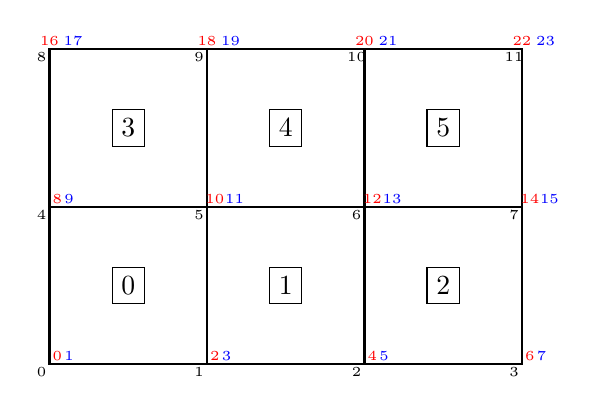
\begin{tikzpicture}
%\draw[step=0.5cm,gray,very thin] (0,0) grid (8,6); %background grid
\draw[thick] (1,1) -- (3,1) -- (3,3) -- (1,3) -- cycle;  
\draw[thick] (3,1) -- (5,1) -- (5,3) -- (3,3) -- cycle; 
\draw[thick] (5,1) -- (7,1) -- (7,3) -- (5,3) -- cycle; 
\draw[thick] (1,3) -- (3,3) -- (3,5) -- (1,5) -- cycle;  
\draw[thick] (3,3) -- (5,3) -- (5,5) -- (3,5) -- cycle; 
\draw[thick] (5,3) -- (7,3) -- (7,5) -- (5,5) -- cycle; 
\node[draw] at (2,2) {0};
\node[draw] at (4,2) {1};
\node[draw] at (6,2) {2};
\node[draw] at (2,4) {3};
\node[draw] at (4,4) {4};
\node[draw] at (6,4) {5};
%pressure dofs
\node at (0.9,0.9) {\tiny 0};
\node at (2.9,0.9) {\tiny 1};
\node at (4.9,0.9) {\tiny 2};
\node at (6.9,0.9) {\tiny 3};
\node at (0.9,2.9) {\tiny 4};
\node at (2.9,2.9) {\tiny 5};
\node at (4.9,2.9) {\tiny 6};
\node at (6.9,2.9) {\tiny 7};
\node at (0.9,4.9) {\tiny 8};
\node at (2.9,4.9) {\tiny 9};
\node at (4.9,4.9) {\tiny 10};
\node at (6.9,4.9) {\tiny 11};
%velocity dofs
\node[red] at (1.1,1.1) {\tiny 0};  \node[blue] at (1.25,1.1) {\tiny 1};
\node[red] at (3.1,1.1) {\tiny 2};  \node[blue] at (3.25,1.1) {\tiny 3};
\node[red] at (5.1,1.1) {\tiny 4};  \node[blue] at (5.25,1.1) {\tiny 5};
\node[red] at (7.1,1.1) {\tiny 6};  \node[blue] at (7.25,1.1) {\tiny 7};
\node[red] at (1.1,3.1) {\tiny 8};  \node[blue] at (1.25,3.1) {\tiny 9};
\node[red] at (3.1,3.1) {\tiny 10}; \node[blue] at (3.35,3.1) {\tiny 11};
\node[red] at (5.1,3.1) {\tiny 12}; \node[blue] at (5.35,3.1) {\tiny 13};
\node[red] at (7.1,3.1) {\tiny 14}; \node[blue] at (7.35,3.1) {\tiny 15};
\node[red] at (1.,5.1) {\tiny 16}; \node[blue] at (1.3,5.1) {\tiny 17};
\node[red] at (3.,5.1) {\tiny 18}; \node[blue] at (3.3,5.1) {\tiny 19};
\node[red] at (5.,5.1) {\tiny 20}; \node[blue] at (5.3,5.1) {\tiny 21};
\node[red] at (7.,5.1) {\tiny 22}; \node[blue] at (7.3,5.1) {\tiny 23};
\end{tikzpicture}\\
{\tiny Red color corresponds to the dofs in the x direction, blue color indicates a dof in the y direction.}
\end{center}

We have nnp=12, nel=6, NfemV=24. Let us assume that free slip boundary conditions are applied. 
The boundary conditions {\tt fix\_bc} array is then:
\begin{center}
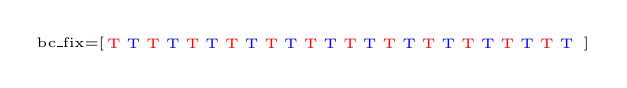
\begin{tikzpicture}
%\draw[step=0.5cm,gray,very thin] (0,0) grid (9,0.7); %background grid
\node  at (0.45,.1) {\tiny bc\_fix=[};

\node[red]  at (1.00,.1) {\tiny T};
\node[blue] at (1.25,.1) {\tiny T};
\node[red]  at (1.50,.1) {\tiny T};
\node[blue] at (1.75,.1) {\tiny T};
\node[red]  at (2.00,.1) {\tiny T};
\node[blue] at (2.25,.1) {\tiny T};
\node[red]  at (2.50,.1) {\tiny T};
\node[blue] at (2.75,.1) {\tiny T};
\node[red]  at (3.00,.1) {\tiny T};
\node[blue] at (3.25,.1) {\tiny T};
\node[red]  at (3.50,.1) {\tiny T};
\node[blue] at (3.75,.1) {\tiny T};
\node[red]  at (4.00,.1) {\tiny T};
\node[blue] at (4.25,.1) {\tiny T};
\node[red]  at (4.50,.1) {\tiny T};
\node[blue] at (4.75,.1) {\tiny T};
\node[red]  at (5.00,.1) {\tiny T};
\node[blue] at (5.25,.1) {\tiny T};
\node[red]  at (5.50,.1) {\tiny T};
\node[blue] at (5.75,.1) {\tiny T};
\node[red]  at (6.00,.1) {\tiny T};
\node[blue] at (6.25,.1) {\tiny T};
\node[red]  at (6.50,.1) {\tiny T};
\node[blue] at (6.75,.1) {\tiny T};

\node  at (7,.1) {\tiny ]};

\end{tikzpicture}\\
\end{center}
Note that since corners belong to two edges, we effectively prescribed 
no-slip boundary conditions on those. 
\todo[inline]{why does array contain only T??}


We wish to compute the tractions on the boundaries, and more precisely for the dofs for which 
a Dirichlet velocity boundary condition has been prescribed.
The number of (traction) unknowns NfemTr is then the number of {\tt T} in the {\tt bc\_fix} array.
In our specific case, we wave NfemTr= .
\todo{finish}
This means that we need for each targeted dof to be able to find its identity/number
between 0 and NfemTr-1. We therefore create the array {\tt bc\_nb} which is 
filled as follows: 
 
\begin{center}
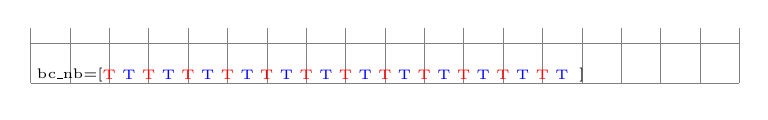
\begin{tikzpicture}
\draw[step=0.5cm,gray,very thin] (0,0) grid (9,0.7); %background grid

\node  at (0.5,.1) {\tiny bc\_nb=[};

\node[red]  at (1.00,.1) {\tiny T};
\node[blue] at (1.25,.1) {\tiny T};
\node[red]  at (1.50,.1) {\tiny T};
\node[blue] at (1.75,.1) {\tiny T};
\node[red]  at (2.00,.1) {\tiny T};
\node[blue] at (2.25,.1) {\tiny T};
\node[red]  at (2.50,.1) {\tiny T};
\node[blue] at (2.75,.1) {\tiny T};
\node[red]  at (3.00,.1) {\tiny T};
\node[blue] at (3.25,.1) {\tiny T};
\node[red]  at (3.50,.1) {\tiny T};
\node[blue] at (3.75,.1) {\tiny T};
\node[red]  at (4.00,.1) {\tiny T};
\node[blue] at (4.25,.1) {\tiny T};
\node[red]  at (4.50,.1) {\tiny T};
\node[blue] at (4.75,.1) {\tiny T};
\node[red]  at (5.00,.1) {\tiny T};
\node[blue] at (5.25,.1) {\tiny T};
\node[red]  at (5.50,.1) {\tiny T};
\node[blue] at (5.75,.1) {\tiny T};
\node[red]  at (6.00,.1) {\tiny T};
\node[blue] at (6.25,.1) {\tiny T};
\node[red]  at (6.50,.1) {\tiny T};
\node[blue] at (6.75,.1) {\tiny T};
\node  at (7,.1) {\tiny ]};
\end{tikzpicture}\\
\end{center}

This translates as follows in the code:
\begin{lstlisting}
NfemTr=np.sum(bc_fix)
bc_nb=np.zeros(NfemV,dtype=np.int32)
counter=0
for i in range(0,NfemV):
    if (bc_fix[i]):
       bc_nb[i]=counter
       counter+=1
\end{lstlisting}


The algorithm is then as follows

\begin{itemize}
\item[A] Prepare two arrays to store the matrix $M_{cbf}$ and its right hand side $rhs_{cbf}$  

\item[B] 
Loop over all elements 

\item[C] 
For each element touching a boundary, compute the residual vector 
$R_{el}=-f_{el} + \K_{el}{\cal V}_{el} + \G_{el} {\cal P}_{el}$

\item[D]
Loop over the four edges of the element using the connectivity array

\item[E]
For each edge loop over the number of degrees of freedom (2 in 2D)

\item[F] 
For each edge assess whether the dofs on both ends are target dofs. 

\item[G]
If so, compute the mass matrix $M_{edge}$ for this edge 

\item[H] extract the 2 values off the element residual vector and assemble these
in $rhs_{cbf}$

\item[I] Assemble $M_{edge}$ into NfemTrxNfemTr matrix using bc\_nb
\end{itemize}


\begin{lstlisting}
M_cbf = np.zeros((NfemTr,NfemTr),np.float64)         # A
rhs_cbf = np.zeros(NfemTr,np.float64)

for iel in range(0,nel):                             # B

    ... compute elemental residual ...               # C

    #boundary 0-1                                    # D
    for i in range(0,ndofV):                         # E
        idof0=2*icon[0,iel]+i
        idof1=2*icon[1,iel]+i
        if (bc_fix[idof0] and bc_fix[idof1]):        # F
           idofTr0=bc_nb[idof0]   
           idofTr1=bc_nb[idof1]
           rhs_cbf[idofTr0]+=res_el[0+i]             # H
           rhs_cbf[idofTr1]+=res_el[2+i]              
           M_cbf[idofTr0,idofTr0]+=M_edge[0,0]       # 
           M_cbf[idofTr0,idofTr1]+=M_edge[0,1]       # I
           M_cbf[idofTr1,idofTr0]+=M_edge[1,0]       # 
           M_cbf[idofTr1,idofTr1]+=M_edge[1,1]       #

    #boundary 1-2                                    #[D]

    ...

    #boundary 2-3                                    #[D]

    ...

    #boundary 3-0                                    #[D]

    ...


\end{lstlisting}










 %------------------

\newpage %---------------------------------------------------------------------
\subsection{The value of the timestep} The chosen time step dt used for time integration is chosen to
comply with the Courant-Friedrichs-Lewy condition \cite{cfd_anderson}.
\begin{equation}
\delta t = C \min \left( \frac{h}{\max |{\bm v}|} , \frac{h^2}{\kappa}  \right)
\end{equation}
where $h$ is a measure of the element size, $\kappa = k/ \rho c_p$ 
is the thermal diffusivity and C is the so-called CFL number chosen in $[0,1[$.

In essence the CFL condition arises when solving hyperbolic PDEs \index{hyperbolic PDE}.
It limits the time step in many explicit time-marching computer simulations
so that the simulation does not produce incorrect results. 

This condition is not needed when solving the Stokes equation but it is mandatory 
when solving the heat transport equation or any kind of advection-diffusion equation. 
Note that any increase of grid resolution (i.e. $h$ becomes smaller) yields an automatic 
decrease of the time step value.






 %---------------------------


\newpage
\subsection{Static condensation} \index{static condensation}



\newpage
\subsection{mappings}

\index{isoparametric}
The name isoparametric derives from the fact that the same ('iso') 
functions are used as basis functions and for the mapping to the reference element. 


\newpage
\subsection{Exporting data to vtk format}

This format seems to be the universally accepted format for 2D and 3D visualisation in 
Computational Geodynamics. Such files can be opened with free softwares such as 
Paraview \footnote{https://www.paraview.org/}, MayaVi \footnote{https://docs.enthought.com/mayavi/mayavi/}
or Visit \footnote{https://wci.llnl.gov/simulation/computer-codes/visit/}.

Unfortunately it is my experience that no simple tutorial exists about how to build 
such files. There is an official document which describes the vtk 
format\footnote{https://www.vtk.org/wp-content/uploads/2015/04/file-formats.pdf}
but it delivers the information in a convoluted way. I therefore describe hereafter 
how \fieldstone{} builds the vtk files. 

I hereunder show vtk file corresponding to the 3x2 grid presented earlier \ref{subsection_meshes}.
In this particular example there are:
\begin{itemize}
\item 12 nodes and 6 elements
\item 1 elemental field: the pressure {\tt p})
\item 2 nodal fields: 1 scalar (the smoothed pressure {\tt q}), 1 vector (the velocity field {\tt u,v,0})
\end{itemize}
Note that vtk files are inherently 3D so that even in the case of a 2D simulation the $z$-coordinate 
of the points and for instance their $z$-velocity component must be provided.
The file, usually called {\sl solution.vtu} starts with a header:

\lstinputlisting[language=python,firstline=1,lastline=3]{images/vtk/solution.vtu}

We then proceed to write the node coordinates as follows:

\lstinputlisting[language=python,firstline=4,lastline=19]{images/vtk/solution.vtu}

These are followed by the elemental field(s):

\lstinputlisting[language=python,firstline=20,lastline=29]{images/vtk/solution.vtu}

Nodal quantities are written next:

\lstinputlisting[language=python,firstline=30,lastline=59]{images/vtk/solution.vtu}

To these informations we must append 3 more datasets. The first one is the connectivity, 
the second one is the offsets and the third one is the type. The first one is trivial
since said connectivity is needed for the Finite Elements. The second must be understood as follows:
when reading the connectivity information in a linear manneer the offset values 
indicate the beginning of each element (omitting the zero value). The third simply is the type of element 
as given in the vtk format document (9 corresponds to a generic quadrilateral with an 
internal numbering consistent with ours). 

\lstinputlisting[language=python,firstline=60,lastline=85]{images/vtk/solution.vtu}

The file is then closed with

\lstinputlisting[language=python,firstline=86,lastline=88]{images/vtk/solution.vtu}

The {\sl solution.vtu} file can then be opened with ParaView, MayaVi or Visit and the reader 
is advised to find tutorials online on how to install and use these softwares. 





\newpage
{\bf To Do}:

write about impose bc on el matrix

full compressible 

total energy calculations

constraints

compositions, marker chain

van keken initial value with deformed mesh

free-slip bc on annulus and sphere . See for example p540 Gresho and Sani book.

non-linear rheologies (two layer brick spmw16, tosn15) 

Picard vs Newton

markers

Schur complement approach

periodic boundary conditions

open boundary conditions

free surface 

SUPG

zaleski disk advection

Busse convection pb, compare with aspect 

cvi !!!

pure elastic 

including phase changes (w. R. Myhill)

discontinuous galerkin

nonlinear poiseuille

formatting of code style

navier-stokes ? (LUKAS)

compute strainrate in middle of element or at quad point for punch?

GEO1442 code 

GEO1442 indenter setup in plane ?

in/out flow on sides for lith modelling

Fehlberg RK advection

\noindent Problems to solve:

colorscale 

better yet simple matrix storage ?

write Scott about matching compressible2 setup with his paper

deal with large matrices. 


\newpage
%%%%%%%%%%%%%%%%%%%%%%%%%%%%%%%%%%%%%%%%%%%%%%%%%%%%%%%%%%%%%%%%%%%%%%%%%%%%%%%
\section{{\tt fieldstone}: simple analytical solution \label{f1}}

From \cite{dohu}. In order to illustrate the behavior of selected mixed finite elements in the solution 
of stationary Stokes flow,  we consider a two-dimensional problem 
in the square domain $\Omega=[0,1]\times[0,1]$, which possesses a closed-form analytical 
solution. The problem consists of determining the velocity field ${\bm v} = (u,v)$ and the 
pressure $p$ such that 
\[
-\nu \Delta {\bm v} + {\bm \nabla} p = {\bm b}  \quad\quad {\rm in} \; \Omega
\]
\[
{\bm \nabla} \cdot {\bm v} = 0 \quad\quad {\rm in} \; \Omega
\]
\[
{\bm v}={\bm 0} \quad\quad {\rm on} \; \Gamma
\]
where the fluid viscosity is taken as $\nu=1$. The components of the body force ${\bm b}$ are prescribed as 
\begin{eqnarray}
b_x &=& (12 - 24y) x^4 + (-24 + 48y) x^3 + (-48y + 72y^2 - 48 y^3 + 12) x^2 \nonumber\\
    && + (-2 + 24y -72y^2+48y^3)x + 1-4y + 12y^2-8y^3 \nonumber\\ 
b_y &=& (8 - 48y + 48 y^2) x^3 + (-12 + 72y - 72y^2) x^2  \nonumber\\
    && + (4 - 24y + 48y^2 - 48y^3 + 24y^4) x - 12y^2 + 24y^3 - 12y^4  \nonumber
\end{eqnarray}
With this prescribed body force, the exact solution is 
\begin{eqnarray}
u(x,y) &=& x^2(1- x)^2 (2y - 6y^2 + 4y^3)  \nonumber\\
v(x,y) &=& -y^2 (1 - y)^2 (2x - 6x^2 + 4x^3) \nonumber\\
p(x,y) &=& x(1 -x)- 1/6 \nonumber 
\end{eqnarray}
Note that the pressure obeys $\int_{\Omega} p \; d\Omega = 0$

\fbox{
\parbox{10cm}{{\bf features}
\begin{itemize}
\item $Q_1\times P_0$ element
\item incompressible flow
\item penalty formulation
\item Dirichlet boundary conditions (no-slip)
\item direct solver
\item isothermal
\item isoviscous
\item analytical solution
\end{itemize}
}}

\includegraphics[width=16cm]{python_codes/fieldstone/solution.pdf}

\begin{center}
\includegraphics[width=12cm]{python_codes/fieldstone/errors.pdf}\\
Quadratic convergence for velocity error, 
linear convergence for pressure error, as expected.
\end{center}

ToDo:

pressure normalisation?

different cmat, a la schmalholz

To go further:
\begin{enumerate}
\item make your own analytical solution
\end{enumerate}


\newpage
%%%%%%%%%%%%%%%%%%%%%%%%%%%%%%%%%%%%%%%%%%%%%%%%%%%%%%%%%%%%%%%%%%%%%%%%%%%%%%%
\section{{\tt fieldstone}: Stokes sphere }

Viscosity and density directly computed at the quadrature points.

\fbox{
\parbox{10cm}{{\bf features}
\begin{itemize}
\item $Q_1\times P_0$ element
\item incompressible flow
\item penalty formulation \index{penalty formulation}
\item Dirichlet boundary conditions (free-slip)
\item isothermal
\item non-isoviscous
\item buoyancy-driven flow \index{buoyancy-driven flow}
\item Stokes sphere \index{Stokes sphere}
\end{itemize}
}}

\includegraphics[width=16cm]{python_codes/fieldstone_stokes_sphere/solution.pdf}



\newpage
%%%%%%%%%%%%%%%%%%%%%%%%%%%%%%%%%%%%%%%%%%%%%%%%%%%%%%%%%%%%%%%%%%%%%%%%%%%%%%%
\section{{\tt fieldstone}: Convection in a 2D box}

This benchmark deals with the 2-D thermal convection of a fluid 
of infinite Prandtl number in a rectangular closed cell.
In what follows, I carry out the case 1a, 1b, and 1c experiments as shown in \cite{blbc89}:
steady convection with constant viscosity in a square box.

The temperature is fixed to zero on top and to $\Delta T$ at the bottom, 
with reflecting symmetry at the sidewalls (i.e. $\partial_x T=0$) 
and there are no internal heat sources. 
Free-slip conditions are implemented on all boundaries. 

The Rayleigh number is given by
\begin{equation}
Ra = \frac{\alpha g_y \Delta T h^3 }{\kappa \nu}
=\frac{\alpha g_y \Delta T h^3 \rho^2 c_p}{k \mu}
\end{equation}

In what follows, I use the following parameter values:  %, as given in \cite{krhb12}:
$L_x=L_y=1$,$\rho_0=c_P=k=\mu=1$, $T_0=0$, $\alpha=10^{-2}$, $g=10^{2}Ra$
and I run the model with $Ra=10^4,10^{5}$ and $10^6$.

The initial temperature field is given by 
\begin{equation}
T(x,y)=(1-y) - 0.01\cos(\pi x) \sin(\pi z)
\end{equation}
The perturbation in the initial temperature fields leads to 
a perturbation of the density field and sets the fluid in motion. 

Depending on the initial Rayleigh number, the system ultimately reaches a 
steady state after some time. 

The Nusselt number (i.e. the mean surface temperature gradient over mean bottom temperature)
is computed as follows \cite{blbc89}:
\begin{equation}
Nu = L_y \frac{\int \frac{\partial T}{\partial y}(y=L_y) dx  }{\int T(y=0) dx}
\label{eqNu}
\end{equation}
Note that in our case the denominator is equal to 1 since $L_x=1$ and the temperature at the 
bottom is prescribed to be 1.

Finally, the steady state root mean square velocity and Nusselt number measurements
are indicated in Table \ref{tab_bl} alongside those of \cite{blbc89} and \cite{tack94}.
(Note that this benchmark was also carried out and published in  
other publications \cite{trha98,albe00,gery10,dawk11,lezh11} but since they did not provide  a complete set
of measurement values, they are not included in the table.)

\begin{center}
\begin{tabular}{llcc}
\hline
          &           & Blankenbach et al & Tackley \cite{tack94}    \\
\hline
\hline
$Ra=10^4$ & $V_{rms}$ &  $42.864947  \pm 0.000020$ & 42.775 \\
          & $Nu$      &  $4.884409   \pm 0.000010$ & 4.878  \\
$Ra=10^5$ & $V_{rms}$ &  $193.21454  \pm 0.00010 $ & 193.11 \\
          & $Nu$      &  $10.534095  \pm 0.000010$ & 10.531 \\
$Ra=10^6$ & $V_{rms}$ &  $833.98977  \pm 0.00020 $ & 833.55 \\
          & $Nu$      &  $21.972465  \pm 0.000020$ & 21.998 \\
\hline
\end{tabular}\\
{\small Steady state Nusselt number $Nu$ and $V_{rms}$ measurements as reported in the literature. }
\end{center}






\fbox{
\parbox{10cm}{{\bf features}
\begin{itemize}
\item $Q_1\times P_0$ element
\item incompressible flow
\item penalty formulation
\item Dirichlet boundary conditions (free-slip)
\item Boussinesq approximation
\item direct solver
\item non-isothermal
\item buoyancy-driven flow
\item isoviscous
\item CFL-condition
\end{itemize}
}}

\includegraphics[width=16cm]{python_codes/fieldstone_convection_box/solution_convection_box.pdf}

ToDo:

implement steady state criterion

reach steady state

do Ra=1e4, 1e5, 1e6

plot against blankenbach paper and aspect

look at critical Ra number


\newpage
%%%%%%%%%%%%%%%%%%%%%%%%%%%%%%%%%%%%%%%%%%%%%%%%%%%%%%%%%%%%%%%%%%%%%%%%%%%%%%%
\section{{\tt fieldstone}: The lid driven cavity}


The lid driven cavity is a famous Computational Fluid Dynamics test case and 
has been studied in countless publications with a wealth of numerical techniques
(see \cite{ertu09} for a succinct review) and also in the laboratory \cite{kost84}.

It models a plane flow of an isothermal isoviscous fluid in a rectangular (usually square) lid-driven cavity. 
The boundary conditions are indicated in the Fig. \ref{fig_ldc}a. The gravity is set to zero.

%---------------------------------------------------------
\subsection{the lid driven cavity problem ({\tt ldc=0})}
In the standard case, the upper side of the cavity moves in its own plane at unit speed, while the other sides are fixed.
This thereby introduces a discontinuity in the boundary conditions at the two upper corners of the cavity and yields
an uncertainty as to which boundary (side or top) the corner points belong to. 
In this version of the code the top corner nodes are considered to be part of the lid. If these are excluded 
the recovered pressure showcases and extremely large checkboard pattern.

This benchmark is usually dicussed in the context of low to very high Reynolds number with the full 
Navier-Stokes equations being solved (with the noticeable exception of \cite{sagl81a,sagl81b,chpc95,eid2005}
which focus on the Stokes equation). 
In the case of the incompressible Stokes flow, 
the absence of inertia renders this problem instantaneous so that only one time step is needed.

%---------------------------------------------------------
\subsection{the lid driven cavity problem - regularisation I ({\tt ldc=1})}

We avoid the top corner nodes issue altogether by  
prescribing the horizontal velocity of the lid as follows: 
\begin{equation}
u(x)=x^2(1-x)^2.
\end{equation}
In this case the velocity and its first derivative is continuous at the corners. This is the so-called regularised lid-driven cavity problem \cite{piva94}.

%---------------------------------------------------------
\subsection{the lid driven cavity problem - regularisation II ({\tt ldc=2})}

Another regularisation was presented in \cite{dejn16}. 
Here, a regularized lid driven cavity is studied which is consistent in the sense that 
${\bm \nabla}\cdot{\bm v}=0$ 
holds also at the corners of the domain.
There are no-slip conditions at the boundaries $x=0$, $x=1$, and $y=0$. 

The velocity at $y=1$ is given by

\begin{eqnarray}
u(x) &=& 1-\frac{1}{4}\left( 1-\cos (\frac{x_1-x}{x_1}\pi)  \right)^2   \quad\quad x\in[0,x_1] \nonumber\\
u(x) &=& 1 \quad\quad x\in[x_1,1-x_1] \nonumber\\
u(x) &=& 1-\frac{1}{4}\left( 1-\cos (\frac{x-(1-x_1)}{x_1}\pi)  \right)^2   \quad\quad x\in[1-x_1,1]
\end{eqnarray}
Results are obtained with $x_1=0.1$.

\begin{center}
\fbox{
\parbox{10cm}{{\bf features}
\begin{itemize}
\item $Q_1\times P_0$ element \index{$Q_1 \times P_0$}
\item incompressible flow
\item penalty formulation \index{penalty formulation}
\item isothermal \index{isothermal}
\item isoviscous \index{isoviscous}
\end{itemize}
}}
\end{center}



\newpage
A 100x100 element grid is used. No-slip boundary conditions are prescribed on sides and
bottom. A zero vertical velocity is prescribed at the top and the exact form of the 
prescribed horizontal velocity is controlled by the {\tt ldc} parameter.

\begin{center}
\includegraphics[width=8cm]{python_codes/fieldstone_lid_driven_cavity/results/p.pdf}\\
\includegraphics[width=12cm]{python_codes/fieldstone_lid_driven_cavity/results/velocities}\\
\includegraphics[width=12cm]{python_codes/fieldstone_lid_driven_cavity/results/pressures}
\end{center}




\newpage
%%%%%%%%%%%%%%%%%%%%%%%%%%%%%%%%%%%%%%%%%%%%%%%%%%%%%%%%%%%%%%%%%%%%%%%%%%%%%%%
\section{{\tt fieldstone}: solcx benchmark}

%Taken from aspect manual. 
The SolCx benchmark is intended to test the accuracy of the solution to a problem that has a large jump in the viscosity along a line through the domain. Such situations are common in geophysics: for example, the viscosity in a cold, subducting slab is much larger than in the surrounding, relatively hot mantle material.

The SolCx benchmark computes the Stokes flow field of a fluid driven by spatial density variations, subject to a spatially variable viscosity. Specifically, the domain is $\Omega = [0,1]^2$, gravity is ${\bm g} = (0,-1)^T$ and the density is given by 
\begin{equation}
\rho(x,y) = \sin(\pi y) \cos(\pi x)
\end{equation}
Boundary conditions are free slip on all of the sides of the domain and the temperature plays no role in this benchmark. 
The viscosity is prescribed as follows:
\begin{equation}
\mu(x,y) = 
\left\{
\begin{array}{lll}
1 & for & x<0.5 \\
10^6 & for & x>0.5 \\
\end{array}
\right.
\end{equation}
Note the strongly discontinuous viscosity field yields a stagnant flow 
in the right half of the domain and thereby yields a pressure discontinuity along the interface. 

The SolCx benchmark was previously used in \cite{dumg11} (references to earlier uses of the benchmark are available there) and its analytic solution is given in \cite{zhon96}. It has been carried out in \cite{krhb12} and \cite{gemd13}. 
Note that the source code which evaluates the velocity and pressure fields for both SolCx and SolKz is 
distributed as part of the open source package Underworld (\cite{moql07}, http://underworldproject.org).

In this particular example, the viscosity is computed analytically at the quadrature points (i.e. tracers are 
not used to attribute a viscosity to the element). 
If the number of elements is even in any direction, all elements (and their associated quadrature points)
have a constant viscosity($1$ or  $10^6$). If it is odd, then the elements situated 
at the viscosity jump have half their integration points with $\mu=1$ and half with $\mu=10^6$ 
(which is a pathological case since the used quadrature rule inside elements cannot represent 
accurately such a jump).  

\fbox{
\parbox{10cm}{{\bf features}
\begin{itemize}
\item $Q_1\times P_0$ element
\item incompressible flow
\item penalty formulation
\item Dirichlet boundary conditions (free-slip)
\item direct solver
\item isothermal
\item non-isoviscous
\item analytical solution
\end{itemize}
}}

\includegraphics[width=16cm]{python_codes/fieldstone_solcx/solution.pdf}

\fbox{
\parbox{10cm}{{\bf What we learn from this}
}}





\newpage
%%%%%%%%%%%%%%%%%%%%%%%%%%%%%%%%%%%%%%%%%%%%%%%%%%%%%%%%%%%%%%%%%%%%%%%%%%%%%%%
\section{{\tt fieldstone}: solkz benchmark}

The SolKz benchmark \cite{repa87} is similar to the SolCx benchmark.
but the viscosity is now a function of the space coordinates: 
\begin{equation}
\mu(y)=\exp(By) \quad {\rm with} \quad B=13.8155
\end{equation}
It is however not a discontinuous function but grows exponentially with the vertical coordinate so that its overall variation is again $10^6$. 
The forcing is again chosen by imposing a spatially variable density variation as follows:
\begin{equation}
\rho(x,y)=\sin(2y) \cos(3\pi x)
\end{equation}
Free slip boundary conditions are imposed on all sides of the domain.
This benchmark is presented in \cite{zhon96} as well and is studied in \cite{dumg11} and \cite{gemd13}.

\includegraphics[width=12cm]{python_codes/fieldstone_solkz/solution.pdf}

\includegraphics[width=8cm]{python_codes/fieldstone_solkz/errors.pdf}


\newpage
%%%%%%%%%%%%%%%%%%%%%%%%%%%%%%%%%%%%%%%%%%%%%%%%%%%%%%%%%%%%%%%%%%%%%%%%%%%%%%%
\section{{\tt fieldstone}: solvi benchmark}

Following SolCx and SolKz, the SolVi inclusion benchmark solves 
a problem with a discontinuous viscosity field, but in this case 
the viscosity field is chosen in such a way that the discontinuity 
is along a circle. Given the regular nature of the grid used by a majority of codes and the present one, 
this ensures that the discontinuity in the viscosity never aligns to cell boundaries.
This in turns leads to almost discontinuous pressures along the interface which are difficult to represent accurately.
\cite{scpo03} derived a simple analytic solution for the pressure and velocity fields for a circular 
inclusion under simple shear and it was used in \cite{deka08}, \cite{sunh10}, \cite{dumg11}, \cite{krhb12} and \cite{gemd13}.

Because of the symmetry of the problem, we only have to solve over the top right quarter of the domain (see Fig. \ref{fig_inclusion1}a). 

The analytical solution requires a strain rate boundary condition (e.g., pure shear) to be applied far away 
from the inclusion. In order to avoid using very large domains and/or dealing with this type of boundary condition altogether, 
the analytical solution is evaluated and imposed on the boundaries of the domain. 
By doing so, the truncation error introduced while discretizing the strain rate boundary condition is removed.

A characteristic of the analytic solution is that the pressure is zero inside the inclusion, while outside it follows the relation
\begin{equation}
p_m = 4 \dot{\epsilon}
\frac{\mu_m(\mu_i-\mu_m)}{\mu_i+\mu_m}
\frac{r_i^2}{r^2} \cos(2\theta)
\end{equation}
where $\mu_i = 10^3$ is the viscosity of the inclusion and $\mu_m = 1$ is the viscosity of the background media, $\theta=\tan^{-1}(y/x)$,
and $\dot{\epsilon}=1$ is the applied strain rate.

\cite{deka08} thoroughly investigated this problem with various numerical methods (FEM, FDM), with and without tracers, 
and conclusively showed how various averagings lead to different results. 
\cite{dumg11} obtained a first order convergence for both pressure and velocity, while \cite{krhb12}
and \cite{gemd13} showed that the use of adaptive mesh refinement in respectively the FEM and FDM 
yields convergence rates which depend on refinement strategies. 

\includegraphics[width=15cm]{python_codes/fieldstone_solvi/solution}


\includegraphics[width=8cm]{python_codes/fieldstone_solvi/errors}


\newpage
%%%%%%%%%%%%%%%%%%%%%%%%%%%%%%%%%%%%%%%%%%%%%%%%%%%%%%%%%%%%%%%%%%%%%%%%%%%%%%%
\section{{\tt fieldstone}: the indentor benchmark}

The punch benchmark is one of the few boundary value problems involving plastic solids for which there exists an exact solution. 
Such solutions are usually either for highly simplified geometries (spherical or axial symmetry, for instance) or simplified material models (such as rigid plastic solids) \cite{kacha04}.

In this experiment, a rigid punch indents a rigid plastic half space; the slip line field theory gives 
exact solutions as shown in Fig. \ref{fig_punch}a. 
The plane strain formulation of the equations and the detailed solution to the problem were derived in the Appendix of \cite{thfb08} and are also presented in \cite{gepd98}.

The two dimensional punch problem has been extensively studied numerically for the past 40 years 
\cite{zihl75,zihp95,chpe01,chan99,huhy99,yuti06,bufs08,raab07} and has been used to draw a parallel with the tectonics of eastern China in the context of the 
India-Eurasia collision \cite{tamo76,mota77}.
It is also worth noting that it has been carried out in one form or another in series of 
analogue modelling articles 
concerning the same region, with a rigid indenter colliding with a rheologically stratified lithosphere \cite{peta88,daco88,jodc90}.

 
Numerically, the one-time step punch experiment is performed on a two-dimensional
domain of purely plastic von Mises material. 
Given that the von Mises rheology yield criterion does not depend on pressure, the density of the material and/or the gravity vector is set to zero. Sides are set to free slip boundary conditions, the bottom to no slip, while a vertical velocity $(0,-v_p)$ is prescribed at the top boundary for nodes whose $x$ coordinate is within $[L_x/2-\delta/2,L_x/2+\delta/2]$. 

The following parameters are used: $L_x=1$, $L_y=0.5$, $\mu_{min}=10^{-3}$, 
$\mu_{max}=10^3$, $v_p=1$, $\delta=0.123456789$ 
and the yield value of the material is set to $k=1$. 

The analytical solution predicts that the angle of the shear bands stemming from the sides of the punch 
is $\pi/4$, that the pressure right under the punch is $1+\pi$, 
and that the velocity of the rigid blocks on each side of the punch is $v_p/\sqrt{2}$ 
(this is simply explained by invoking conservation of mass).

\includegraphics[width=16cm]{python_codes/fieldstone_indentor/solution.pdf}

ToDo: smooth punch

\fbox{
\parbox{10cm}{{\bf features}
\begin{itemize}
\item $Q_1\times P_0$ element \index{$Q_1 \times P_0$}
\item incompressible flow \index{incompressible flow}
\item penalty formulation \index{penalty formulation}
\item Dirichlet boundary conditions (no-slip)
\item isothermal \index{isothermal}
\item non-isoviscous \index{non-isoviscous}
\item nonlinear rheology \index{nonlinear rheology}
\end{itemize}
}}



\newpage
%%%%%%%%%%%%%%%%%%%%%%%%%%%%%%%%%%%%%%%%%%%%%%%%%%%%%%%%%%%%%%%%%%%%%%%%%%%%%%%
\section{{\tt fieldstone}: the annulus benchmark}
This benchmark is based on Thieulot \& Puckett [Subm.] in which an analytical solution to the
isoviscous incompressible Stokes equations is derived in an annulus geometry.
The velocity and pressure fields are as follows:

\begin{eqnarray}
v_r(r,\theta)     &=&  g(r) k \sin(k\theta), \\
v_\theta(r,\theta)&=&  f(r) \cos(k \theta), \\ 
p(r,\theta)       &=&  k h(r) \sin(k \theta), \\
\rho (r,\theta)   &=& \aleph(r) k \sin (k \theta), 
\end{eqnarray}
with
\begin{eqnarray}
f(r)&=&Ar+B/r, \\
g(r) &=& \frac{A}{2}r  +  \frac{B}{r} \ln r + \frac{C}{r}, \\
h(r)&=& \frac{2g(r)-f(r)}{r},  \\
\aleph(r) &=& g'' - \frac{g'}{r}  - \frac{g}{r^2} (k^2 - 1)  + \frac{f}{r^2}   + \frac{f'}{r}, \\
A &=& -C\frac{2(\ln R_1 - \ln R_2)} { R_2^2 \ln R_1  - R_1^2 \ln R_2}, \\
B &=& -C \frac{R_2^2-R_1^2}{R_2^2 \ln R_1 - R_1^2 \ln R_2}.
\end{eqnarray}

The parameters $A$ and $B$ are chosen so that $v_r(R_1)=v_r(R_2)=0$, i.e.
the velocity is tangential to both inner and outer surfaces.
The gravity vector is radial and of unit length.
In the present case, we set $R_1=1$, $R_2=2$ and $C=-1$. 

\fbox{
\parbox{10cm}{{\bf features}
\begin{itemize}
\item $Q_1\times P_0$ element
\item incompressible flow
\item penalty formulation
\item Dirichlet boundary conditions
\item direct solver
\item isothermal
\item isoviscous
\item analytical solution
\item annulus geometry
\item elemental boundary conditions
\end{itemize}
}}

\includegraphics[width=6cm]{python_codes/fieldstone_annulus/density}
\includegraphics[width=6cm]{python_codes/fieldstone_annulus/pressure}
\includegraphics[width=6cm]{python_codes/fieldstone_annulus/velocity}

\includegraphics[width=16cm]{python_codes/fieldstone_annulus/errors}




\newpage
%%%%%%%%%%%%%%%%%%%%%%%%%%%%%%%%%%%%%%%%%%%%%%%%%%%%%%%%%%%%%%%%%%%%%%%%%%%%%%%
\section{{\tt fieldstone}: stokes sphere (3D) - penalty\label{f5}}

\fbox{
\parbox{10cm}{{\bf features}
\begin{itemize}
\item $Q_1\times P_0$ element
\item incompressible flow
\item penalty formulation
\item Dirichlet boundary conditions (free-slip)
\item direct solver
\item isothermal
\item non-isoviscous
\item 3D
\item elemental b.c. 
\item buoyancy driven
\end{itemize}
}}


\begin{center}
\includegraphics[width=5cm]{python_codes/fieldstone_stokes_sphere_3D/grid}
\includegraphics[width=5cm]{python_codes/fieldstone_stokes_sphere_3D/vel}
\includegraphics[width=5cm]{python_codes/fieldstone_stokes_sphere_3D/press}\\
\includegraphics[width=5cm]{python_codes/fieldstone_stokes_sphere_3D/press2}
\includegraphics[width=5cm]{python_codes/fieldstone_stokes_sphere_3D/visc}
\includegraphics[width=5cm]{python_codes/fieldstone_stokes_sphere_3D/dens}\\
{\small resolution is 24x24x24}
\end{center}



\newpage
%%%%%%%%%%%%%%%%%%%%%%%%%%%%%%%%%%%%%%%%%%%%%%%%%%%%%%%%%%%%%%%%%%%%%%%%%%%%%%%
\section{{\tt fieldstone}: stokes sphere (3D) - mixed formulation\label{f5}}

This is the same setup as Section \ref{f5}.

\fbox{
\parbox{10cm}{{\bf features}
\begin{itemize}
\item $Q_1\times P_0$ element
\item incompressible flow
\item mixed formulation
\item Dirichlet boundary conditions (free-slip)
\item direct solver
\item isothermal
\item non-isoviscous
\item 3D
\item elemental b.c. 
\item buoyancy driven
\end{itemize}
}}



\newpage
%%%%%%%%%%%%%%%%%%%%%%%%%%%%%%%%%%%%%%%%%%%%%%%%%%%%%%%%%%%%%%%%%%%%%%%%%%%%%%%
\section{{\tt fieldstone}: consistent pressure recovery }
What follows is presented in \cite{zina82}. The second part of their paper wishes to establish a simple
and effective numerical method to calculate variables eliminated by the penalisation process. 
The method involves an additional finite element solution for the nodal pressures using 
the same finite element basis and numerical quadrature as used for the velocity.

Let us start with:
\[
p = -\lambda {\bm \nabla}\cdot {\bm v}
\]
which lead to
\[
(q,p)=-\lambda (q,{\bm \nabla}\cdot{\bm v})
\]
and then
\[
\left( \int {\bm N} {\bm N} d\Omega \right) \cdot {\bm P} = - \left( \lambda \int {\bm N} {\bm \nabla}{\bm N} d\Omega \right)\cdot{\bm V}
\]
or, 
\[
{\bm M} \cdot {\bm P} = - {\bm D}\cdot{\bm V}
\]
and finally
\[
{\bm P} = -{\bm M}^{-1} \cdot {\bm D} \cdot {V}
\]
with ${\bm M}$ of size $(np\times np)$, ${\bm D}$ of size $(np*ndof\times np*ndof)$ and ${\bm V}$ of size $(np*ndof)$.
The vector ${\bm P}$ contains the $np$ nodal pressure values directly, with no need for a smoothing scheme. 
The mass matrix ${\bm M}$ is to be evaluated at the full integration points, while the constraint part (the right
hand side of the equation) is to be evaluated at the reduced integration point. 

As noted by \cite{zina82}, it is interesting to note that when linear elements are used and the lumped matrices
are used for the ${\bm M}$ the resulting algebraic equation is identical to the smoothing scheme based
on the averaging method only if the uniform square finite element mesh is used. 
In this respect this method is expected to yield different results when elements are not square or even rectangular.

-------

$q_1$ is smoothed pressure obtained with the  center-to-node approach.

$q_2$ is recovered pressure obtained with \cite{zina82}.

All three fulfill the zero average condition: $\int p d\Omega = 0$.

\includegraphics[width=15cm]{python_codes/fieldstone_consistent_pressure_recovery/solution}

\includegraphics[width=8cm]{python_codes/fieldstone_consistent_pressure_recovery/errors}

In terms of pressure error, $q_2$ is better than $q_1$ which is better than elemental.

QUESTION: why are the averages exactly zero ?!

TODO: 
\begin{itemize}
\item add randomness to internal node positions.
\item look at elefant algorithms
\end{itemize}


\newpage
%%%%%%%%%%%%%%%%%%%%%%%%%%%%%%%%%%%%%%%%%%%%%%%%%%%%%%%%%%%%%%%%%%%%%%%%%%%%%%%
\section{{\tt fieldstone}: the Particle in Cell technique (1) - the effect of averaging}



\newpage
%%%%%%%%%%%%%%%%%%%%%%%%%%%%%%%%%%%%%%%%%%%%%%%%%%%%%%%%%%%%%%%%%%%%%%%%%%%%%%%
\section{{\tt fieldstone}: solving the full saddle point problem}
The details of the numerical setup are presented in Section \ref{f1}.

The main difference is that we no longer use the penalty formulation and therefore 
keep both velocity and pressure as unknowns. Therefore we end up having to solve 
the following system:
\[
\left(
\begin{array}{cc}
\K & \G \\ \G^T & 0 
\end{array}
\right)
\cdot
\left(
\begin{array}{c}
V \\ P
\end{array}
\right)
=
\left(
\begin{array}{c}
 f \\ h
\end{array}
\right)
\quad\quad
{\rm or,}
\quad\quad
\A \cdot X = rhs
\]
Each block $\K$, $\G$ and vector $f$, $h$ are built separately in the code and assembled into 
the matrix $\A$ and vector $rhs$ afterwards. $\A$ and $rhs$ are then passed to the solver. 
We will see later that there are alternatives to solve this approach which do not require to 
build the full Stokes matrix $\A$. 

Each element has $m=4$ vertices so in total $ndofV\times m=8$ velocity dofs and a single 
pressure dof, commonly situated in the center of the element. The total number of 
velocity dofs is therefore $NfemV=nnp \times ndofV$ while the total number of
pressure dofs is $NfemP=nel$. The total number of dofs is then $Nfem=NfemV+NfemP$.

As a consequence, matrix $\K$ has size $NfemV,NfemV$ and matrix $\G$ has size $NfemV,NfemP$.
Vector $f$ is of size $NfemV$ and vector $h$ is of size $NfemP$.  


\fbox{
\parbox{10cm}{{\bf features}
\begin{itemize}
\item $Q_1\times P_0$ element \index{$Q_1 \times P_0$}
\item incompressible flow \index{incompressible flow}
\item mixed formulation \index{mixed formulation}
\item Dirichlet boundary conditions (no-slip)
\item direct solver (?)
\item isothermal \index{isothermal}
\item isoviscous \index{isoviscous}
\item analytical solution \index{analytical solution}
\item pressure smoothing \index{pressure smoothing} 
\end{itemize}
}}

\includegraphics[width=16cm]{python_codes/fieldstone_saddlepoint/solution.pdf}

Unlike the results obtained with the penalty formualtion (see Section \ref{f1}),
the pressure showcases a very strong checkerboard pattern, similar to the one 
in \cite{dohu05}.

\begin{center}
\includegraphics[width=7cm]{python_codes/fieldstone_saddlepoint/doneahuerta}
\includegraphics[width=7cm]{python_codes/fieldstone_saddlepoint/mine}\\
Left: pressure solution as shown in \cite{dohu05}; Right: pressure solution obtained
with fieldstone.
\end{center}

Rather interestingly, the nodal pressure (obtained with a simple center-to-node algorithm)
fails to recover a correct pressure at the four corners.


\newpage
%%%%%%%%%%%%%%%%%%%%%%%%%%%%%%%%%%%%%%%%%%%%%%%%%%%%%%%%%%%%%%%%%%%%%%%%%%%%%%%
\section{{\tt fieldstone}: solving the full saddle point problem in 3D}

{\color{red} this does not work because of the Dirichlet b.c. on all 6 sides and all three components}
It does work well with Q2Q1.

This benchmark begins by postulating a polynomial solution to the 3D Stokes equation \cite{dobo04}:
\begin{equation}
{\bm v}
=
\left(
\begin{array}{c}
x+x^2+xy+x^3y \\
y + xy + y^2 + x^2 y^2\\
-2z - 3xz - 3yz - 5x^2 yz
\end{array}
\right)
\label{eqbur}
\end{equation}
and
\begin{equation}
p = xyz + x^3 y^3z - 5/32
\end{equation}
While it is then trivial to verify that this velocity field is divergence-free,  
the corresponding body force of the Stokes equation can be computed by 
inserting this solution into the momentum equation with a given viscosity $\mu$
(constant or position/velocity/strain rate dependent). 
The domain is a unit cube and velocity boundary conditions 
simply use Eq. (\ref{eqbur}). 
Following \cite{busa13}, the viscosity
is given by the smoothly varying function
\begin{equation}
\mu = exp(1 - \beta(x(1 - x) + y(1 - y) + z(1 - z)))
\end{equation}
Choosing $\beta=0$ yields a constant velocity $\mu=e^1$ (and greatly simplifies the right-hand side).
One can easily show that the ratio of viscosities $\mu^\star$
in the system follows $\mu^\star=\exp(-3\beta/4)$ so that choosing $\beta=10$ yields
$\mu^\star\simeq 1808$ and $\beta=20$ yields $\mu^\star\simeq 3.269\times10^6$.


We start from the momentum conservation equation:
\[
-{\bm \nabla}p + {\bm \nabla}\cdot (2 \mu \dot{\bm \epsilon}) = {\bm f}
\]
The $x$-component of this equation writes
\begin{eqnarray}
f_x 
&=& -\frac{\partial p}{\partial x} 
+\frac{\partial}{\partial x} (2\mu \dot{\epsilon}_{xx})
+\frac{\partial}{\partial y} (2\mu \dot{\epsilon}_{xy})
+\frac{\partial}{\partial z} (2\mu \dot{\epsilon}_{xz}) \\
&=& 
-\frac{\partial p}{\partial x} 
+2\mu\frac{\partial}{\partial x} \dot{\epsilon}_{xx}
+2\mu\frac{\partial}{\partial y} \dot{\epsilon}_{xy}
+2\mu\frac{\partial}{\partial z} \dot{\epsilon}_{xz} 
+2\frac{\partial \mu}{\partial x} \dot{\epsilon}_{xx}
+2\frac{\partial \mu}{\partial y} \dot{\epsilon}_{xy}
+2\frac{\partial \mu}{\partial z} \dot{\epsilon}_{xz} 
\end{eqnarray}


Let us compute all the block separately:
\begin{eqnarray}
\dot{\epsilon}_{xx}&=& 1+2x+y+3x^2y  \nonumber\\
\dot{\epsilon}_{yy}&=& 1+x+2y+2x^2y \nonumber\\
\dot{\epsilon}_{zz}&=& -2-3x-3y-5x^2y \nonumber\\
2 \dot{\epsilon}_{xy}&=& (x+x^3)+(y+2xy^2) = x+y+2xy^2+x^3 \nonumber\\
2 \dot{\epsilon}_{xz}&=& (0)+(-3z-10xyz) = -3z -10xyz  \nonumber\\
2 \dot{\epsilon}_{yz}&=& (0) + (-3z-5x^2z) = -3z-5x^2z   \nonumber
\end{eqnarray}
In passing, one can verify that 
$
\dot{\epsilon}_{xx}
+\dot{\epsilon}_{yy}
+\dot{\epsilon}_{zz}=0
$.
We further have
\begin{eqnarray}
\frac{\partial}{\partial x} 2\dot{\epsilon}_{xx}&=& 2(2 +6xy) \nonumber\\ 
\frac{\partial}{\partial y} 2\dot{\epsilon}_{xy}&=&  1+4xy \nonumber\\
\frac{\partial}{\partial z} 2\dot{\epsilon}_{xz}&=& -3 -10xy   \nonumber\\ 
\frac{\partial}{\partial x} 2\dot{\epsilon}_{xy}&=& 1+2y^2+3x^2 \nonumber\\ 
\frac{\partial}{\partial y} 2\dot{\epsilon}_{yy}&=& 2( 2+2x^2 ) \nonumber\\ 
\frac{\partial}{\partial z} 2\dot{\epsilon}_{yz}&=& -3-5x^2   \nonumber\\
\frac{\partial}{\partial x} 2\dot{\epsilon}_{xz}&=& -10yz \nonumber\\ 
\frac{\partial}{\partial y} 2\dot{\epsilon}_{yz}&=& 0  \nonumber\\ 
\frac{\partial}{\partial z} 2\dot{\epsilon}_{zz}&=& 2( 0 ) \nonumber
\end{eqnarray}

\begin{eqnarray}
\frac{\partial p}{\partial x} &=& yz+3x^2y^3z\\
\frac{\partial p}{\partial y} &=& xz +3x^3y^2z \\
\frac{\partial p}{\partial z} &=& xy+x^3y^3
\end{eqnarray}

The viscosity is chosen to be 
\[
\mu(x,y,z) = \exp \left[ 1-\beta ( x(1-x)+y(1-y)+z(1-z) )   \right]
\]

%-----------------------------
\paragraph{Constant viscosity}

Setting $\beta=0$ yields 
\[
\mu(x,y,z) = e \simeq 2.718
\]
so that 
\begin{eqnarray}
\frac{\partial }{\partial x} \mu(x,y,z) &=& 0 \\
\frac{\partial }{\partial y} \mu(x,y,z) &=& 0 \\
\frac{\partial }{\partial z} \mu(x,y,z) &=& 0
\end{eqnarray}
and 
\begin{eqnarray}
f_x 
&=& 
-\frac{\partial p}{\partial x} 
+2\mu\frac{\partial}{\partial x} \dot{\epsilon}_{xx}
+2\mu\frac{\partial}{\partial y} \dot{\epsilon}_{xy}
+2\mu\frac{\partial}{\partial z} \dot{\epsilon}_{xz} \nonumber\\
&=&
-(yz+3x^2y^3z)
+ 2(2 +6xy) + (1+4xy) + (-3 -10xy)   \\
&=&
-(yz+3x^2y^3z)
+\mu(2+6xy ) \\
f_y 
&=&  
-\frac{\partial p}{\partial y} 
+2\mu\frac{\partial}{\partial x} \dot{\epsilon}_{xy}
+2\mu\frac{\partial}{\partial y} \dot{\epsilon}_{yy}
+2\mu\frac{\partial}{\partial z} \dot{\epsilon}_{yz}  \nonumber\\
&=&
-(xz +3x^3y^2z)
+
\mu(1+2y^2+3x^2)
+\mu2( 2+2x^2 )  
+\mu(-3-5x^2) \\
&=&
-(xz +3x^3y^2z)
+ \mu ( 2 + 2x^2 +  2y^2)
\\ 
f_z 
&=&
-\frac{\partial p}{\partial z} 
+2\mu\frac{\partial}{\partial x} \dot{\epsilon}_{xz}
+2\mu\frac{\partial}{\partial y} \dot{\epsilon}_{yz}
+2\mu\frac{\partial}{\partial z} \dot{\epsilon}_{zz}  \nonumber\\
&=&
-(xy+x^3y^3) 
+ \mu (-10yz) + 0 + 0 \\
&=&
-(xy+x^3y^3) 
+\mu (-10yz) 
\end{eqnarray}

finally

\[
{\bm f} = 
-
\left(
\begin{array}{c}
yz+3x^2y^3z\\
xz +3x^3y^2z \\
xy+x^3y^3
\end{array}
\right)
+\mu
\left(
\begin{array}{c}
2+6xy  \\
2 + 2x^2 +  2y^2 \\
-10yz 
\end{array}
\right)
\]

$\Rightarrow$ sign problem with Burstedde et al Eq 26 !!



%-----------------------------
\paragraph{Variable viscosity}

\begin{eqnarray}
\frac{\partial }{\partial x} \mu(x,y,z) &=& -(1-2x)\beta \mu(x,y,z) \nonumber\\
\frac{\partial }{\partial y} \mu(x,y,z) &=& -(1-2y)\beta \mu(x,y,z) \nonumber\\
\frac{\partial }{\partial z} \mu(x,y,z) &=& -(1-2z)\beta \mu(x,y,z) \nonumber
\end{eqnarray}

\begin{eqnarray}
{\bm f} 
&=& 
-
\left(
\begin{array}{c}
yz+3x^2y^3z\\
xz +3x^3y^2z \\
xy+x^3y^3
\end{array}
\right)
+\mu
\left(
\begin{array}{c}
2+6xy  \\
2 + 2x^2 +  2y^2 \\
-10yz 
\end{array}
\right) \\
&&
-(1-2x)\beta \mu (x,y,z)
\left(
\begin{array}{c}
2\dot{\epsilon}_{xx} \\
2\dot{\epsilon}_{xy} \\
2\dot{\epsilon}_{xz} \\
\end{array}
\right)
-(1-2y)\beta \mu (x,y,z)
\left(
\begin{array}{c}
2\dot{\epsilon}_{xy} \\
2\dot{\epsilon}_{yy} \\
2\dot{\epsilon}_{yz} \\
\end{array}
\right)
-(1-2z)\beta \mu (x,y,z)
\left(
\begin{array}{c}
2\dot{\epsilon}_{xz} \\
2\dot{\epsilon}_{yz} \\
2\dot{\epsilon}_{zz} \\
\end{array}
\right) \nonumber\\
&=& 
-
\left(
\begin{array}{c}
yz+3x^2y^3z\\
xz +3x^3y^2z \\
xy+x^3y^3
\end{array}
\right)
+\mu
\left(
\begin{array}{c}
2+6xy  \\
2 + 2x^2 +  2y^2 \\
-10yz 
\end{array}
\right) \nonumber\\
&-&
(1-2x)\beta \mu 
\left(
\begin{array}{c}
2+4x+2y+6x^2y \\
x+y+2xy^2+x^3 \\
-3z -10xyz 
\end{array}
\right)
-(1-2y)\beta \mu 
\left(
\begin{array}{c}
x+y+2xy^2+x^3 \\
2+2x+4y+4x^2y \\
-3z-5x^2z \\
\end{array}
\right)
-(1-2z)\beta \mu
\left(
\begin{array}{c}
-3z -10xyz \\
-3z-5x^2z \\
-4-6x-6y-10x^2y
\end{array}
\right) \nonumber
\end{eqnarray}

at $(x,y,z)=(0,0,0)$, $\mu=\exp(1)$, 

at $(x,y,z)=(0.5,0.5,0.5)$, $\mu=\exp(1-3\beta/4)$

Viscosity ratio is given by 
\[
\mu^\star = \frac{\exp(1-3\beta/4)}{\exp(1)} = \exp(-3\beta/4)
\]
By varying $\beta$ between 1 and 22 we can get up to 7 orders of magnitude viscosity difference !

























\fbox{
\parbox{10cm}{{\bf features}
\begin{itemize}
\item $Q_1\times P_0$ element
\item incompressible flow
\item saddle point system
\item Dirichlet boundary conditions (free-slip)
\item direct solver
\item isothermal
\item non-isoviscous
\item 3D
\item elemental b.c. 
\item analytical solution
\end{itemize}
}}


%\begin{center}
%\includegraphics[width=5cm]{python_codes/fieldstone_stokes_sphere_3D/grid}
%\includegraphics[width=5cm]{python_codes/fieldstone_stokes_sphere_3D/vel}
%\includegraphics[width=5cm]{python_codes/fieldstone_stokes_sphere_3D/press}\\
%\includegraphics[width=5cm]{python_codes/fieldstone_stokes_sphere_3D/press2}
%\includegraphics[width=5cm]{python_codes/fieldstone_stokes_sphere_3D/visc}
%\includegraphics[width=5cm]{python_codes/fieldstone_stokes_sphere_3D/dens}\\
%{\small resolution is 24x24x24}
%\end{center}



\newpage
%%%%%%%%%%%%%%%%%%%%%%%%%%%%%%%%%%%%%%%%%%%%%%%%%%%%%%%%%%%%%%%%%%%%%%%%%%%%%%%
\section{{\tt fieldstone}: solving the full saddle point problem with $Q_2\times Q_1$ elements}
The details of the numerical setup are presented in Section \ref{f1}.

Each element has $m_V=9$ vertices so in total $ndof_V\times m_V=18$ velocity dofs and 
$ndof_P*m_P=4$ pressure dofs. The total number of 
velocity dofs is therefore $NfemV=nnp \times ndofV$ while the total number of
pressure dofs is $NfemP=nel$. The total number of dofs is then $Nfem=NfemV+NfemP$.

As a consequence, matrix $\K$ has size $NfemV,NfemV$ and matrix $\G$ has size $NfemV,NfemP$.
Vector $f$ is of size $NfemV$ and vector $h$ is of size $NfemP$.  

\begin{center}
\includegraphics[width=12cm]{python_codes/fieldstone_saddlepoint_q2q1/q2q1setup}\\
{\color{red} renumber all nodes to start at zero!! Also internal numbering does not work here }
\end{center}


ToDo:
\begin{itemize}
\item normalise pressure 
\end{itemize}

\fbox{
\parbox{10cm}{{\bf features}
\begin{itemize}
\item $Q_2\times Q_1$ element \index{$Q_2 \times Q_1$}
\item incompressible flow \index{incompressible flow}
\item mixed formulation \index{mixed formulation}
\item Dirichlet boundary conditions (no-slip)
\item isothermal \index{isothermal}
\item isoviscous \index{isoviscous}
\item analytical solution \index{analytical solution}
\end{itemize}
}}

\begin{center}
\includegraphics[width=10cm]{python_codes/fieldstone_saddlepoint_q2q1/errors}
\end{center}


\newpage
%%%%%%%%%%%%%%%%%%%%%%%%%%%%%%%%%%%%%%%%%%%%%%%%%%%%%%%%%%%%%%%%%%%%%%%%%%%%%%%
\section{{\tt fieldstone}: solving the full saddle point problem with $Q_3\times Q_2$ elements}
The details of the numerical setup are presented in Section \ref{f1}.

Each element has $m_V=16$ vertices so in total $ndof_V\times m_V=32$ 
velocity dofs and 
$ndof_P*m_P=9$ pressure dofs. The total number of 
velocity dofs is therefore $NfemV=nnp \times ndofV$ while the total number of
pressure dofs is $NfemP=nel$. The total number of dofs is then $Nfem=NfemV+NfemP$.

As a consequence, matrix $\K$ has size $NfemV,NfemV$ and matrix $\G$ has size $NfemV,NfemP$.
Vector $f$ is of size $NfemV$ and vector $h$ is of size $NfemP$.  

\begin{verbatim}

60===61===62===63===64===65===66===67===68===70
||             ||             ||             ||
50   51   52   53   54   55   56   57   58   59
||             ||             ||             ||
40   41   42   43   44   45   46   47   48   49
||             ||             ||             ||
30===31===32===33===34===35===36===37===38===39
||             ||             ||             ||
20   21   22   23   24   25   26   27   28   29
||             ||             ||             ||
10   11   12   13   14   15   16   17   18   19
||             ||             ||             ||
00===01===02===03===04===05===06===07===08===09

Example of 3x2 mesh. nnx=10, nny=7, nnp=70, nelx=3, nely=2, nel=6
\end{verbatim}


\begin{verbatim}
12===13===14===15           06=====07=====08
||   ||   ||   ||           ||     ||     ||
08===09===10===11           ||     ||     ||
||   ||   ||   ||           03=====04=====05
04===05===06===07           ||     ||     ||
||   ||   ||   ||           ||     ||     ||
00===01===02===03           00=====01=====02

Velocity (Q3)               Pressure (Q2)

(r,s)_{00}=(-1,-1)          (r,s)_{00}=(-1,-1) 
(r,s)_{01}=(-1/3,-1)        (r,s)_{01}=(0,-1) 
(r,s)_{02}=(+1/3,-1)        (r,s)_{02}=(+1,-1) 
(r,s)_{03}=(+1,-1)          (r,s)_{03}=(-1,0) 
(r,s)_{04}=(-1,-1/3)        (r,s)_{04}=(0,0) 
(r,s)_{05}=(-1/3,-1/3)      (r,s)_{05}=(+1,0) 
(r,s)_{06}=(+1/3,-1/3)      (r,s)_{06}=(-1,+1) 
(r,s)_{07}=(+1,-1/3)        (r,s)_{07}=(0,+1) 
(r,s)_{08}=(-1,+1/3)        (r,s)_{08}=(+1,+1) 
(r,s)_{09}=(-1/3,+1/3)
(r,s)_{10}=(+1/3,+1/3)
(r,s)_{11}=(+1,+1/3)
(r,s)_{12}=(-1,+1)
(r,s)_{13}=(-1/3,+1)
(r,s)_{14}=(+1/3,+1)
(r,s)_{15}=(+1,+1)

\end{verbatim}



The velocity shape functions are given by:
\begin{eqnarray}
N_1(r)&=&(-1   +r +9r^2 - 9r^3)/16 \nonumber\\
N_2(r)&=&(+9 -27r -9r^2 +27r^3)/16 \nonumber\\
N_3(r)&=&(+9 +27r -9r^2 -27r^3)/16 \nonumber\\
N_4(r)&=&(-1   -r +9r^2 + 9r^3)/16 \nonumber
\end{eqnarray}

\begin{eqnarray}
N_1(t)&=&(-1   +t +9t^2 - 9t^3)/16 \nonumber\\
N_2(t)&=&(+9 -27t -9t^2 +27t^3)/16 \nonumber\\
N_3(t)&=&(+9 +27t -9t^2 -27t^3)/16 \nonumber\\
N_4(t)&=&(-1   -t +9t^2 + 9t^3)/16 \nonumber
\end{eqnarray}

\begin{eqnarray}
N_01(r,t)&=&N_1(r)N_1(t) \\
N_02(r,t)&=&N_2(r)N_1(t) \\
N_03(r,t)&=&N_3(r)N_1(t) \\
N_04(r,t)&=&N_4(r)N_1(t) \\
N_05(r,t)&=&N_1(r)N_2(t) \\
N_06(r,t)&=&N_2(r)N_2(t) \\
N_07(r,t)&=&N_3(r)N_2(t) \\
N_08(r,t)&=&N_4(r)N_2(t) \\
N_09(r,t)&=&N_1(r)N_3(t) \\
N_10(r,t)&=&N_2(r)N_3(t) \\
N_11(r,t)&=&N_3(r)N_3(t) \\
N_12(r,t)&=&N_4(r)N_3(t) \\
N_13(r,t)&=&N_1(r)N_4(t) \\
N_14(r,t)&=&N_2(r)N_4(t) \\
N_15(r,t)&=&N_3(r)N_4(t) \\
N_16(r,t)&=&N_4(r)N_4(t) 
\end{eqnarray}

and their derivatives:






{\color{red} Write about 4 point quadrature}.








\fbox{
\parbox{10cm}{{\bf features}
\begin{itemize}
\item $Q_3\times Q_2$ element \index{$Q_3 \times Q_2$}
\item incompressible flow \index{incompressible flow}
\item mixed formulation \index{mixed formulation}
\item isothermal \index{isothermal}
\item isoviscous \index{isoviscous}
\item analytical solution \index{analytical solution}
\end{itemize}
}}

\begin{center}
\includegraphics[width=10cm]{python_codes/fieldstone_saddlepoint_q3q2/errors}
\end{center}

velocity error rate is cubic, pressure superconvergent since the pressure field
is quadratic and therefore lies into the Q2 space.


\newpage
%%%%%%%%%%%%%%%%%%%%%%%%%%%%%%%%%%%%%%%%%%%%%%%%%%%%%%%%%%%%%%%%%%%%%%%%%%%%%%%
\section{{\tt fieldstone}: the Busse benchmark}

This three-dimensional benchmark was first proposed by \cite{bucc93}. 
It has been subsequently presented in \cite{tack94,trha98,albe00,omma06,dawk11,krhb12}.
We here focus on Case 1 of \cite{bucc93}:  an isoviscous bimodal convection experiment at $Ra=3\times 10^5$.

The domain is of size $a\times b\times h$ with $a=1.0079h$, $b=0.6283h$ with $h=2700$km. It is filled with a Newtonian fluid
characterised by $\rho_0=3300{\rm kg}.{\rm m}^{-3}$, $\alpha=10^{-5}{\rm K}^{-1}$, $\mu=8.0198\times10^{23}{\rm Pa.s}$, 
$k=3.564{\rm W}.{\rm m}^{-1}.{\rm K}^{-1}$, 
$c_p=1080{\rm J}.{\rm K}^{-1}.{\rm kg}^{-1}$.
The gravity vector is set to ${\bm g}=(0,0,-10)^T$.
The temperature is imposed at the bottom  ($T=3700^\circ$C) and at the top ($T=0^\circ$C).

The various measurements presented in \cite{bucc93} are listed hereafter:
\begin{itemize}
\item The Nusselt number $Nu$ computed at the top surface following Eq. (\ref{eqNu}):
\[
Nu = L_z \frac{\int\int_{z=L_z} \frac{\partial T}{\partial y} dx dy  }{\int \int_{z=0} T dx dy}
\]
\item the root mean square velocity $v_{rms}$ and the temperature mean square velocity $T_{rms}$
\item The vertical velocity $w$ and temperature $T$ at points ${\bm x}_1=(0,0,L_z/2)$, ${\bm x}_2=(L_x,0,L_z/2)$,
${\bm x}_3=(0,L_y,L_z/2)$ and ${\bm x}_4=(L_x,L_y,L_z/2)$;
\item the vertical component of the heat flux $Q$ at the top surface  at all four corners.
\end{itemize}

The values plotted hereunder are adimensionalised by means of a reference temperature (3700K),
a reference lengthscale 2700km, and a reference time $L_z^2/\kappa$. 




\fbox{
\parbox{10cm}{{\bf features}
\begin{itemize}
\item $Q_1\times P_0$ element
\item incompressible flow
\item mixed formulation
\item Dirichlet boundary conditions (free-slip)
\item direct solver
\item isothermal
\item non-isoviscous
\item 3D
\item elemental b.c. 
\item buoyancy driven
\end{itemize}
}}




\newpage
%%%%%%%%%%%%%%%%%%%%%%%%%%%%%%%%%%%%%%%%%%%%%%%%%%%%%%%%%%%%%%%%%%%%%%%%%%%%%%%
\section{{\tt fieldstone}: The non-conforming $Q_1 \times P_0$ element} \label{ncq1p0} 


\fbox{
\parbox{10cm}{{\bf features}
\begin{itemize}
\item Non-conforming $Q_1\times P_0$ element \index{nonconforming $Q_1 \times P_0$}
\item incompressible flow \index{incompressible flow}
\item mixed formulation \index{mixed formulation}
\item isothermal \index{isothermal}
\item non-isoviscous \index{non-isoviscous}
\item analytical solution \index{analytical solution}
\item pressure smoothing \index{pressure smoothing} 
\end{itemize}
}}

try Q1 mapping instead of isoparametric.

%\includegraphics[width=16cm]{python_codes/fieldstone_saddlepoint/solution.pdf}



\newpage
%%%%%%%%%%%%%%%%%%%%%%%%%%%%%%%%%%%%%%%%%%%%%%%%%%%%%%%%%%%%%%%%%%%%%%%%%%%%%%%
\section{{\tt fieldstone}: The stabilised $Q_1 \times Q_1$ element} 
The details of the numerical setup are presented in Section \ref{f1}.



\newpage
%%%%%%%%%%%%%%%%%%%%%%%%%%%%%%%%%%%%%%%%%%%%%%%%%%%%%%%%%%%%%%%%%%%%%%%%%%%%%%%
\section{{\tt fieldstone}: compressible flow (1)}
We first start with an isothermal Stokes flow, so that we disregard the heat transport equation and 
the equations we wish to solve are simply:

\begin{align}
  \label{eq:stokes-1}
  -\nabla \cdot \left[2\eta \left(\dot\varepsilon(\bm v)
                                  - \frac{1}{3}(\nabla \cdot \bm v)\mathbf 1\right)
                \right] + \nabla p &=
  \rho \bm g
  &
  & \textrm{in $\Omega$},
  \\
  \label{eq:stokes-2}
  \nabla \cdot (\rho \bm v) &= 0
  &
  & \textrm{in $\Omega$}
\end{align}
The second equation can be rewritten 
$\nabla \cdot (\rho {\bm v}) =  \rho \nabla \cdot {\bm v} + {\bm v} \cdot {\bm \nabla}\rho=0$
or, 
\[
\nabla \cdot {\bm v} + \frac{1}{\rho} {\bm v} \cdot {\bm \nabla}\rho=0
\]
Note that this presupposes that the density is not zero anywhere in the domain.

We use a mixed formulation and therefore  
keep both velocity and pressure as unknowns. We end up having to solve 
the following system:
\[
\left(
\begin{array}{cc}
\K & \G \\ \G^T+\Z & 0 
\end{array}
\right)
\cdot
\left(
\begin{array}{c}
{\cal V} \\ {\cal P}
\end{array}
\right)
=
\left(
\begin{array}{c}
 f \\ h
\end{array}
\right)
\quad\quad
{\rm or,}
\quad\quad
\A \cdot X = rhs
\]
Where $\K$ is the stiffness matrix, $\G$ is the discrete gradient operator, 
$\G^T$ is the discrete divergence operator, ${\cal V}$ the velocity vector, 
${\cal P}$ the pressure vector.
Note that the term $\Z{\cal V}$ derives from term ${\bm v} \cdot {\bm \nabla} \rho$ in the continuity equation. 

Each block $\K$, $\G$ , $\Z$ and vectors $f$ and $h$ are built separately 
in the code and assembled into 
the matrix $\A$ and vector $rhs$ afterwards. $\A$ and $rhs$ are then passed to the solver. 
We will see later that there are alternatives to solve this approach which do not require to 
build the full Stokes matrix $\A$. 

{\sl Remark}: the term $\Z {\cal V}$ is often put in the rhs (i.e. added to $h$) so that 
the matrix $\A$ retains the same structure as in the incompressible case. This is indeed 
how it is implemented in ASPECT. 

In the case of a compressible flow the strain rate tensor and the deviatoric strain rate tensor are no more equal (since ${\bm \nabla}\cdot{\bm v} \neq 0$).
The deviatoric strainrate tensor is given by\footnote{See the ASPECT manual for a justification of the 3 value in the denominator in 2D and 3D.} 
\[
\dot{\bm \epsilon}^d({\bm v})=
\dot{\bm \epsilon}({\bm v})-\frac{1}{3} Tr(\dot{\bm \epsilon}) {\bm 1}
=\dot{\bm \epsilon}({\bm v})-\frac{1}{3} ({\bm \nabla}\cdot{\bm v}) {\bm 1}
\]
In that case:
\begin{eqnarray}
\dot{\epsilon}_{xx}^d 
&=& \frac{\partial u}{\partial x}
-\frac{1}{3} \left( \frac{\partial u}{\partial x} + \frac{\partial v}{\partial y} \right) 
= \frac{2}{3}\frac{\partial u}{\partial x}
-\frac{1}{3} \frac{\partial v}{\partial y}
%=
%\frac{2}{3} \sum_{i=1}^4 \frac{\partial N_i}{\partial x}\;  u_i 
%-\frac{1}{3} \sum_{i=1}^4 \frac{\partial N_i}{\partial y}\;  v_i 
\\
\dot{\epsilon}_{yy}^d 
&=& \frac{\partial v}{\partial y}
-\frac{1}{3} \left( \frac{\partial u}{\partial x} + \frac{\partial v}{\partial y} \right) 
=-\frac{1}{3} \frac{\partial u}{\partial x} 
+ \frac{2}{3} \frac{\partial v}{\partial y} 
%=-\frac{1}{3}  \sum_{i=1}^4 \frac{\partial N_i}{\partial x}\;  u_i
%+ \frac{2}{3} \sum_{i=1}^4 \frac{\partial N_i}{\partial y}\;  v_i
\\
2\dot{\epsilon}_{xy}^d 
&=& 
\frac{\partial u}{\partial y} 
+\frac{\partial v}{\partial x} 
%= \sum_{i=1}^4 \frac{\partial N_i}{\partial y}\;  u_i
%+ \sum_{i=1}^4 \frac{\partial N_i}{\partial x}\;  v_i
\end{eqnarray}
and then 
\[
\dot{\bm \epsilon}^d({\bm v})
=
\left(
\begin{array}{cc}
\frac{2}{3} \frac{\partial u}{\partial x} -\frac{1}{3} \frac{\partial v}{\partial y} &
\frac{1}{2}\frac{\partial u}{\partial y} + \frac{1}{2}\frac{\partial v}{\partial x}  \\ \\
\frac{1}{2}\frac{\partial u}{\partial y} + \frac{1}{2}\frac{\partial v}{\partial x}  &
-\frac{1}{3} \frac{\partial u}{\partial x} +\frac{2}{3} \frac{\partial v}{\partial y} 
\end{array}
\right)
\]

From $\vec{\tau} = 2\eta \vec{\epsilon}^d$ we arrive at:
\[
\left(
\begin{array}{c}
\tau_{xx}\\
\tau_{yy}\\
\tau_{xy}\\
\end{array}
\right)
=
2\eta
\left(
\begin{array}{c}
\dot{\epsilon}_{xx}^d \\
\dot{\epsilon}_{yy}^d \\
\dot{\epsilon}_{xy}^d 
\end{array}
\right)
=2 \eta
\left(
\begin{array}{ccc}
2/3 & -1/3& 0 \\
-1/3 & 2/3 & 0 \\
0 & 0 & 1/2 \\
\end{array}
\right)
\cdot 
\left(
\begin{array}{c}
\frac{\partial u}{\partial x} \\ 
\frac{\partial v}{\partial y} \\ 
\frac{\partial u}{\partial y}\! +\! \frac{\partial v}{\partial x} \\
\end{array}
\right)
=
\eta
\left(
\begin{array}{ccc}
4/3 & -2/3& 0 \\
-2/3 & 4/3 & 0 \\
0 & 0 & 1 \\
\end{array}
\right)
\cdot 
\left(
\begin{array}{c}
\frac{\partial u}{\partial x} \\ 
\frac{\partial v}{\partial y} \\ 
\frac{\partial u}{\partial y}\! +\! \frac{\partial v}{\partial x} \\
\end{array}
\right)
\]
or, 
\[
\vec{\tau} = {\bm C}_\eta {\bm B} V
\]


















\newpage
In order to test our implementation we have created a few manufactured solutions:
\begin{itemize}
\item benchmark \#1 ({\tt ibench=1})): Starting from a density profile of:
\begin{equation}
    \rho = xy
\end{equation}
We derive a velocity given by:
\begin{equation}
    v_x = \frac{C_x}{x} , v_y = \frac{C_y}{y}
\end{equation}

With $g_x = \frac{1}{x}$ and $g_y = \frac{1}{y}$, this leads us to a pressure profile:
\begin{equation}
    p = - \mu \left( \frac{C_x}{x^2} + \frac{C_y}{y^2} \right)  + xy + C_0
\end{equation}
This gives us a strain rate:
\begin{align}
    \begin{split}
        e_{xx} =  \frac{-C_x}{x^2}
        \\
        e_{yy} =  \frac{-C_y}{y^2}
    \end{split}
\end{align}

 
\item benchmark \#2 ({\tt ibench=2}): Starting from a density profile of:
\begin{equation}
    \rho = cos(x)cos(y)
\end{equation}
We derive a velocity given by:
\begin{equation}
    v_x = \frac{C_x}{cos(x)} , v_y = \frac{C_y}{cos(y)}
\end{equation}
With $g_x = \frac{1}{cos(x)}$ and $g_y = \frac{1}{cos(y)}$, this leads us to a pressure profile:
\begin{equation}
    p =  \mu \Bigg(\frac{C_x sin(x)}{cos^2(x)} + \frac{C_y sin(y)}{cos^2(y)}\Bigg) 
    -( sin(x) + sin(y) ) + C_0
\end{equation}
\begin{align}
    \begin{split}
        e_{xx} = C_x \frac{sin(x)}{cos^2(x)}
        \\
        e_{yy} = C_y \frac{sin(y)}{cos^2(y)}
    \end{split}
\end{align}



\item benchmark \#3 
\item benchmark \#4 
\item benchmark \#5 
\end{itemize}




\fbox{
\parbox{10cm}{{\bf features}
\begin{itemize}
\item $Q_1\times P_0$ element \index{$Q_1 \times P_0$}
\item incompressible flow \index{incompressible flow}
\item mixed formulation \index{mixed formulation}
\item Dirichlet boundary conditions (no-slip)
\item direct solver (?)
\item isothermal \index{isothermal}
\item isoviscous \index{isoviscous}
\item analytical solution \index{analytical solution}
\item pressure smoothing \index{pressure smoothing} 
\end{itemize}
}}

%\includegraphics[width=16cm]{python_codes/fieldstone_saddlepoint/solution.pdf}




\newpage
%%%%%%%%%%%%%%%%%%%%%%%%%%%%%%%%%%%%%%%%%%%%%%%%%%%%%%%%%%%%%%%%%%%%%%%%%%%%%%%
\section{{\tt fieldstone}: compressible flow (2)}
Let us start with some thermodynamics. Every material has an equation of state.
The equilibrium thermodynamic state of any material can
be constrained if any two state variables are specified.
Examples of state variables include
the pressure $p$ and specific volume $\nu = 1/\rho$, as well as the temperature $T$.

After linearisation, the density depends on temperature and pressure as follows:
\[
\rho(T,p) = \rho_0 \left((1 - \alpha(T-T_0) + \beta_T p \right)
\]
where $\alpha$ is the coefficient of thermal expansion, also called 
thermal expansivity: \index{thermal expansion}
\[
\alpha=-\frac{1}{\rho}\left( \frac{\partial \rho}{\partial T} \right)_p
\]
$\alpha$ is the percentage increase in volume of a material per degree of temperature increase; the
subscript $p$ means that the pressure is held fixed.

$\beta_T$ is the isothermal compressibility of the fluid, which is given by \index{compressibility}
\[
\beta_T = \frac{1}{K} = \frac{1}{\rho}\left( \frac{\partial \rho}{\partial P} \right)_T
\]
with $K$ the bulk modulus. \index{bulk modulus}
%aspect manual
Values of $\beta_T=10^{-12}-10^{-11}$ Pa$^{-1}$ are reasonable for Earth's mantle, with values decreasing by about a
factor of 5 between the shallow lithosphere and core-mantle boundary.
This is the percentage increase in density per unit change in pressure at constant temperature.
Both the coefficient of thermal expansion and the isothermal compressibility can be obtained
from the equation of state.

The full set of equations we wish to solve is given by

\begin{eqnarray}
-\nabla \cdot \left[2\eta \dot{\bm \epsilon}^d({\bm v}) \right] + \nabla p &=& \rho_0 \left((1 - \alpha(T-T_0) + \beta_T p \right) {\bm g} \quad\quad \textrm{in $\Omega$}  \label{eq:stokes-1} \\
\nabla \cdot {\bm v} + \frac{1}{\rho} {\bm v} \cdot {\bm \nabla}\rho&=&0 \quad\quad  \textrm{in $\Omega$}   \label{eq:stokes-2} \\
\rho C_p \left(\frac{\partial T}{\partial t} + \bm v\cdot\nabla T\right) - \nabla\cdot k\nabla T   &=& 
  \rho H  +  2\eta \dot{\bm \epsilon}^d : \dot{\bm \epsilon}^d    +\alpha T \left( \frac{\partial p}{\partial t}+  \bm v \cdot \nabla p \right) 
\quad\quad   \textrm{in $\Omega$},
  \label{eq:temperature}
\end{eqnarray}

Note that this presupposes that the density is not zero anywhere in the domain.

We use a mixed formulation and therefore  
keep both velocity and pressure as unknowns. We end up having to solve 
the following system:
\[
\left(
\begin{array}{cc}
\K & \G+\W \\ \G^T+\Z & 0 
\end{array}
\right)
\cdot
\left(
\begin{array}{c}
{\cal V} \\ {\cal P}
\end{array}
\right)
=
\left(
\begin{array}{c}
 f \\ h
\end{array}
\right)
\quad\quad
{\rm or,}
\quad\quad
\A \cdot X = rhs
\]
Where $\K$ is the stiffness matrix, $\G$ is the discrete gradient operator, 
$\G^T$ is the discrete divergence operator, ${\cal V}$ the velocity vector, 
${\cal P}$ the pressure vector.
Note that the term $\Z{\cal V}$ derives from term ${\bm v} \cdot {\bm \nabla} \rho$ in the continuity equation. 

As perfectly explained in the step 32 of deal.ii\footnote{https://www.dealii.org/9.0.0/doxygen/deal.II/step\_32.html},
we need to scale the $\G$ term since it is many orders of magnitude smaller than $\K$, which introduces large inaccuracies in the solving process to the point that the solution is nonsensical. This scaling coefficient is $\eta/L$. After building the $\G$ block, it is then scaled as follows: $\G'=\frac{\eta}{L}\G$ so that we now solve 

\[
\left(
\begin{array}{cc}
\K & \G'+\W \\ \G'^T+\Z & 0 
\end{array}
\right)
\cdot
\left(
\begin{array}{c}
{\cal V} \\ {\cal P}'
\end{array}
\right)
=
\left(
\begin{array}{c}
 f \\ h
\end{array}
\right)
\]
After the solve phase, we recover the real pressure with ${\cal P}=\frac{\eta}{L}{\cal P}'$.

{\color{red} adapt notes since I should scale $\W$ and $\Z$ too}.
{\color{red} $h$ should be caled too !!!!!!!!!!!!!!!} 

Each block $\K$, $\G$ , $\Z$ and vectors $f$ and $h$ are built separately 
in the code and assembled into 
the matrix $\A$ and vector $rhs$ afterwards. $\A$ and $rhs$ are then passed to the solver. 
We will see later that there are alternatives to solve this approach which do not require to 
build the full Stokes matrix $\A$. 

{\sl Remark 1}: the terms $\Z {\cal V}$ and $\W {\cal P}$ are 
often put in the rhs (i.e. added to $h$) so that 
the matrix $\A$ retains the same structure as in the incompressible case. This is indeed 
how it is implemented in ASPECT, see also appendix A of \cite{lezh08}. This however requires more work since the rhs depends 
on the solution and some form of iterations is needed. 

{\sl Remark 2}: Very often the adiabatic heating term  
$\alpha T \left( \bm v \cdot \nabla p \right)$ is simplified as follows:
%aspect manual
If you assume the vertical component of the gradient of the dynamic pressure to be small compared to the
gradient of the total pressure (in other words, the gradient is dominated by the gradient of the hydrostatic
pressure), then $-\rho {\bm g} \simeq {\bm \nabla}p$ and then 
$\alpha T \left( \bm v \cdot \nabla p \right) \simeq  -\alpha\rho T {\bm v}\cdot{\bm g}$. We will however 
not be using this approximation in what follows.



We have already established that
\[
\vec{\tau} = {\bm C}_\eta {\bm B} V
\]




\newpage
The setup is as follows: the domain is $Lx=Ly=3000$km. Free slip boundary conditions are imposed on all four sides. 
The initial temperature is given by:
\[
T(x,y) = \left(  \frac{L_y-y}{Ly} - 0.01\cos(\frac{\pi x}{L_x}) \sin(\frac{\pi y}{Ly}) \right) \Delta T + T_0
\]
with $\Delta T=4000$K, $T_0=273.15$K. The temperature is set to $\Delta T + T_0$ at the bottom and $T_0$ at the top.
We also set $k=3$, $C_p=1250$, $|g|=10$, $\rho_0=3000$ and we keep the Rayleigh number $Ra$ and dissipation number $Di$ as input parameters:
\[
Ra=\frac{\alpha g \Delta T L^3 \rho_0^2 C_p}{\eta k}
\quad\quad
Di=\frac{\alpha g L}{C_p}
\]
From the second equation we get $\alpha=\frac{Di C_p}{g L}$, which we can insert in the first one:
\[
Ra=\frac{Di C_p^2 \Delta T L^2 \rho_0^2 }{\eta k}
\quad\quad
{\rm or,}
\quad\quad
\eta=
\frac{Di C_p^2 \Delta T L^2 \rho_0^2 }{Ra \; k  }
\]
For instance, for $Ra=10^4$ and $Di=0.75$, we obtain $\alpha\simeq 3\cdot 10^{-5}$ and $\eta\simeq 10^{25}$ 
which are quite reasonable values. 



{\color{red} WRITE ABOUT REF VALUES }






The following measurements are carried out:
\begin{itemize}
\item The root mean square velocity:
\[
v_{rms} = \sqrt{\frac{1}{V}\int_V v^2 dV   }
\]
\item The average temperature:
\[
<T>=\frac{1}{V}\int_V T dV
\]
\item The total mass:
\[
M=\int_V \rho dV
\]
\item The Nusselt number:
\[
Nu=-\frac{1}{Lx}\frac{1}{\Delta T} \int_0^{L_x} \frac{\partial T(x,y=L_y)}{\partial y} dx
\]
\item The kinetic energy:
\[
E_K=\int_V \frac{1}{2}\rho v^2 dV
\]
\item The work done against gravity
\[
<W>=-\int_V \rho g_y v_y dV
\]
\item The total viscous dissipation
\[
<\Phi>=\int \Phi dV =\frac{1}{V}\int 2 \eta \dot{\bm \varepsilon}:\dot{\bm \varepsilon} dV 
\]
\item The gravitational potential energy (GPE)
\[
E_G = \int_V \rho g_y (L_y-y) dV
\]
\item The internal thermal energy
\[
E_T = \int_V \rho C_p T dV
\]


\end{itemize}

\newpage

Following \cite{lezh08}, we multiply the momentum equation by ${\bm v}$ and integrate over the whole volume:
\[
\int_V {\bm v} \cdot \left[ -\nabla \cdot {\bm \tau}  + \nabla p \right] dV  = \int_V {\bm v} \cdot \rho {\bm g} dV
\]
or, 
\[
-\int_V {\bm v} \cdot \nabla \cdot {\bm \tau} dV +\int_V {\bm v} \cdot  \nabla p dV  = \int_V {\bm v} \cdot \rho {\bm g} dV
\]
Let us look at each block separately:
\[
-\int_V {\bm v} \cdot \nabla \cdot {\bm \tau} dV  
=-\int_S  {\bm \tau} \underbrace{{\bm v}\cdot {\bm n}}_{=0 \; (b.c.)} dS + \int_V {\bm \nabla}{\bm v} : {\bm \tau} dV 
= \int_V \dot{\bm \varepsilon} : {\bm \tau} dV 
= \int_V \Phi  dV 
\]
which is the volume integral of the shear heating. Then,
\[
\int_V {\bm v} \cdot  \nabla p dV  =
\int_S p \underbrace{{\bm v}\cdot {\bm n}}_{=0 \; (b.c.)} dS - \int_V {\bm \nabla}\cdot{\bm v} \; p dV  
\]
which is zero in the case of an incompressible flow. {\color{red} expand when compressible}.
And finally
\[
\int_V {\bm v} \cdot \rho {\bm g} dV = W
\]
which is the work against gravity. \index{work against gravity} 

Conclusion for an incompressible fluid: we should have
\[
\int_V \Phi  dV 
=
\int_V {\bm v} \cdot \rho {\bm g} dV 
\]

{\color{red} pressure disappears completely from there, so that whether full pressure or reduced
pressure is used it yields the same equation, which is impossible since the lith pressure is not 
altering the flow (i.e. not changing $\Phi$) but the responsible $\rho_0$ will offset the 
work against gravity.} This works in the code provided the work is computed with $\rho-rho_0$...

\newpage
Following the Reynold's transport theorem \cite{malvern},p210, we have for a property $A$ (per unit mass)
\[
\frac{d}{dt} \int_V A \rho dV = \int_V \frac{\partial }{\partial t} (A\rho) dV + \int_S A \rho {\bm v}\cdot {\bm n} dS
\]
Let us apply to this to $A=C_p T$:
\begin{eqnarray}
\frac{d}{dt} \int_V \rho C_p T dV 
&=& \int_V \frac{\partial }{\partial t} (\rho C_p T ) dV + \int_S A \rho \underbrace{{\bm v}\cdot {\bm n}}_{=0 \; (b.c.)} dS \\
&=& \int_V C_p T \frac{\partial \rho}{\partial t} dV + \int_V \rho C_p \frac{\partial T}{\partial t}  dV 
\end{eqnarray}


\begin{eqnarray}
\int_V \rho C_p \frac{\partial T}{\partial t}  dV
&=&  
+ \int_V \left[ -\rho C_p {\bm v}\cdot {\bm \nabla}T +{\bm \nabla}\cdot k {\bm \nabla} T + \rho H  + \Phi    +\alpha T \left( \frac{\partial p}{\partial t}+  \bm v \cdot {\bm \nabla} p \right) \right]  dV \\ 
&=& 
+ \int_V \left[ -\rho C_p {\bm v}\cdot {\bm \nabla}T 
+ \rho H  + \Phi    +\alpha T \left( \frac{\partial p}{\partial t}+  \bm v \cdot {\bm \nabla} p \right) \right]  dV 
+ \int_V {\bm \nabla}\cdot k {\bm \nabla} T dV \\ 
&=& 
+ \int_V \left[ -\rho C_p {\bm v}\cdot {\bm \nabla}T 
+ \rho H  + \Phi    +\alpha T \left( \frac{\partial p}{\partial t}+  \bm v \cdot {\bm \nabla} p \right) \right]  dV 
+ \int_S  k {\bm \nabla} T \cdot {\bm n}  dS \\ 
&=& 
+ \int_V \left[ -\rho C_p {\bm v}\cdot {\bm \nabla}T 
+ \rho H  + \Phi    +\alpha T \left( \frac{\partial p}{\partial t}+  \bm v \cdot {\bm \nabla} p \right) \right]  dV 
- \int_S  {\bm q} \cdot {\bm n}  dS 
\\
\\
 \int_V C_p T \frac{\partial \rho}{\partial t} dV
&=& 
- \int_V C_p T {\bm \nabla} \cdot (\rho {\bm v}) dV
=
-\int_V C_p T \rho \underbrace{{\bm v} \cdot {\bm n}}_{=0 \; (b.c.)} dS +  \int_V \rho C_p  {\bm \nabla}  T \cdot {\bm v} dV
\end{eqnarray}

Finally:

\begin{eqnarray}
\frac{d}{dt} \int_V \rho C_p T dV 
 &=& 
 \int_V \left[ 
 \rho H  + \Phi    +\alpha T \left( \frac{\partial p}{\partial t}+  \bm v \cdot {\bm \nabla} p \right) \right]  dV 
- \int_S  {\bm q} \cdot {\bm n}  dS \\ 
\end{eqnarray}



\newpage
\fbox{
\parbox{10cm}{{\bf features}
\begin{itemize}
\item $Q_1\times P_0$ element \index{$Q_1 \times P_0$}
\item compressible flow \index{compressible flow}
\item mixed formulation \index{mixed formulation}
\item Dirichlet boundary conditions (no-slip)
\item isoviscous \index{isoviscous}
\item analytical solution \index{analytical solution}
\item pressure smoothing \index{pressure smoothing} 
\end{itemize}
}}

Relevant literature: \cite{itki94,tagu07,lezh08,kilv10,lezh11,lizh13,hedg17}

%\includegraphics[width=16cm]{python_codes/fieldstone_saddlepoint/solution.pdf}




\newpage
%%%%%%%%%%%%%%%%%%%%%%%%%%%%%%%%%%%%%%%%%%%%%%%%%%%%%%%%%%%%%%%%%%%%%%%%%%%%%%%
\section{{\tt fieldstone}: Rayleigh-Taylor instability (1)}
This numerical experiment was first presented in \cite{vkks97}.
It consists of an isothermal Rayleigh-Taylor instability in a two-dimensional box
of size $Lx=0.9142$ and $L_y=1$.

\begin{center}
\includegraphics[width=7cm]{python_codes/fieldstone_RTinstability1/images/setup}
\end{center}

Two Newtonian fluids are present in the system: the buoyant layer is placed at the bottom of 
the box and the interface between both fluids is given by 
$
y(x)=0.2+0.02\cos \left( \frac{\pi x}{L_x}  \right)
$
The bottom fluid is parametrised by its mass density $\rho_1$ and its viscosity $\mu_1$, 
while the layer above is parametrised by $\rho_2$ and $\mu_2$.

No-slip boundary conditions are applied at the bottom and at the top of the box 
while free-slip boundary conditions are applied on the sides. 

In the original benchmark the system is run over 2000 units of dimensionless time and the 
timing and position of various upwellings/downwellings is monitored. 
In this present experiment only the root mean square velocity is measured at $t=0$:
the code is indeed not yet foreseen of any algorithm capable of tracking deformation.

Another approach than the ones presented in the extensive literature which showcases 
results of this benchmark is taken. The mesh is initially fitted to the fluids
interface and the resolution is progressively increased. This results in the 
following figure:

\begin{center}
\includegraphics[width=7cm]{python_codes/fieldstone_RTinstability1/images/grid}
\includegraphics[width=8cm]{python_codes/fieldstone_RTinstability1/images/vrms.pdf}
\end{center}
The green line indicates results obtained with my code ELEFANT with grids up to 2000x2000
with the exact same methodology.

\begin{center}
\includegraphics[width=4cm]{python_codes/fieldstone_RTinstability1/images/vel_128}
\includegraphics[width=4cm]{python_codes/fieldstone_RTinstability1/images/exx_128}
\includegraphics[width=4cm]{python_codes/fieldstone_RTinstability1/images/exy_128}
\includegraphics[width=4cm]{python_codes/fieldstone_RTinstability1/images/eyy_128}
\end{center}







\fbox{
\parbox{10cm}{{\bf features}
\begin{itemize}
\item $Q_1\times P_0$ element \index{$Q_1 \times P_0$}
\item incompressible flow \index{incompressible flow}
\item mixed formulation \index{mixed formulation}
\item isothermal \index{isothermal}
\item numerical benchmark \index{numerical benchmark}
\end{itemize}
}}



\newpage
%%%%%%%%%%%%%%%%%%%%%%%%%%%%%%%%%%%%%%%%%%%%%%%%%%%%%%%%%%%%%%%%%%%%%%%%%%%%%%%
\section{{\tt fieldstone}: Slab detachment benchmark (1)}

As in \cite{schm11}, the computational domain is $1000km \times 660km$.
No-slip boundary conditions are imposed on the sides of the system while free-slip
boundary conditions are imposed at the top and bottom.
Two materials are present in the domain: the lithosphere (mat.1) and the mantle (mat.2). 
The overriding plate (mat.1) is $80km$ thick and is placed at the top of the domain. 
An already subducted slab (mat.1) of $250km$ length hangs vertically under this plate.
The mantle occupies the rest of the domain.

The mantle has a constant viscosity $\eta_0=10^{21}Pa.s$ and a density $\rho=3150kg/m^3$. 
The slab has a density $\rho=3300kg/m^3$ and is characterised by a power-law flow law so that 
its effective viscosity depends on the second invariant of the strainrate $I_2$ as follows:

\begin{equation}
\eta_{eff}
=\frac{1}{2} A^{-1/n_s} I_2^{1/n_s-1} 
=\frac{1}{2} [(2 \times 4.75\!\times\! 10^{11})^{-n_s}]^{-1/n_s} I_2^{1/n_s-1} 
=4.75\!\times\! 10^{11} I_2^{1/n_s-1} 
= \eta_0 I_2^{1/n_s-1} 
\end{equation}
with 
$n_s=4$ and $A=(2 \times 4.75\!\times\! 10^{11})^{-n_s}$, or $\eta_0=4.75\times 10^{11}$.




\begin{center}
\includegraphics[width=5.cm]{python_codes/fieldstone_slab_detachment1/images/151/density}
\includegraphics[width=5.cm]{python_codes/fieldstone_slab_detachment1/images/151/velocity}
\includegraphics[width=5.cm]{python_codes/fieldstone_slab_detachment1/images/151/viscosity}\\
Fields at convergence for 151x99 grid.
\end{center}




\begin{center}
\includegraphics[width=7cm]{python_codes/fieldstone_slab_detachment1/images/horizontal.pdf}
\includegraphics[width=7cm]{python_codes/fieldstone_slab_detachment1/images/horizontal_zoom.pdf}\\
\includegraphics[width=7cm]{python_codes/fieldstone_slab_detachment1/images/vertical.pdf}
\includegraphics[width=7cm]{python_codes/fieldstone_slab_detachment1/images/residual.pdf}
\end{center}

\begin{center}
\includegraphics[width=5cm]{python_codes/fieldstone_slab_detachment1/images/horizontal_exx.pdf}
\includegraphics[width=5cm]{python_codes/fieldstone_slab_detachment1/images/horizontal_eyy.pdf}
\includegraphics[width=5cm]{python_codes/fieldstone_slab_detachment1/images/horizontal_exy.pdf}\\
Along the horizontal line
\end{center}

\begin{center}
\includegraphics[width=5cm]{python_codes/fieldstone_slab_detachment1/images/vertical_exx.pdf}
\includegraphics[width=5cm]{python_codes/fieldstone_slab_detachment1/images/vertical_eyy.pdf}
\includegraphics[width=5cm]{python_codes/fieldstone_slab_detachment1/images/vertical_exy.pdf}\\
Along the vertical line
\end{center}



\fbox{
\parbox{10cm}{{\bf features}
\begin{itemize}
\item $Q_1\times P_0$ element \index{$Q_1 \times P_0$}
\item incompressible flow \index{incompressible flow}
\item mixed formulation \index{mixed formulation}
\item isothermal \index{isothermal}
\item nonlinear rheology \index{nonlinear}
\item nonlinear residual
\end{itemize}
}}

Todo: nonlinear mantle, pressure normalisation 



%\newpage
%\subsection{Using MUMPS}
%\subsection{With periodic boundary conditions}
%\subsection{Different Cmat}
%\subsection{Penalty Uzawa formulation}
%\subsection{Powell-Hestenes iterations a la MILAMIN}
%\subsection{With temperature and phase change}
%\subsection{Conformal refinement}
%\subsection{Newton vs Picard solver}
%\subsection{With markers}
%\subsection{Stress b.c.}
%\subsection{open boundary conditions}
%\subsection{melt generation}
%after Schmeling paper
%\subsection{Consistent pressure recovery}
%\subsection{Uzawa outer scheme}
%\subsection{PCG outer scheme}

\appendix

\newpage
%%%%%%%%%%%%%%%%%%%%%%%%%%%%%%%%%%%%%%%%%%%%%%%%%%%%%%%%%%%%%%%%%%%%%%%%%%%%%%%
%\section{The main codes in computational geodynamics}
%
In what follows I make a quick inventory of the main codes of computational geodynamics, 
for crust, lithosphere and/or mantle modelling.

in order to find all CIG-codes citations go to: https://geodynamics.org/cig/news/publications-refbase/

\begin{itemize}

%------------------------------------------------------------------------------
\item {\codefont ABAQUS} \index{general}{ABAQUS code}
%------------------------------------------------------------------------------

{\small
\noindent
\cite{brry01}
\cite{gedh02}
\cite{fumr03}
\cite{hapf06}
\cite{camg07}
\cite{kuhe09}
\cite{makh09}
\cite{camg10}
\cite{nalr12}
\cite{pevp15}
\cite{naam17}
\cite{naam18}
}

%------------------------------------------------------------------------------
\item {\codefont ANSYS} \index{general}{ANSYS code}
%------------------------------------------------------------------------------

\cite{nehe06}
\cite{guyr16}

%------------------------------------------------------------------------------
\item {\codefont ADELI} \index{general}{ADELI code}
%------------------------------------------------------------------------------

{\small
\noindent
1997: \cite{hajc97}\\
2001: \cite{chzh01}\\
2004: \cite{gocl04}\\
2006: \cite{vech06}\cite{golc06}\\
2008: \cite{boht08a}\cite{boht08b}\\
2012: \cite{gech12}\cite{gigh12}\\
2013: \cite{wahd13}\\
2014: \cite{cehg14}\\
2015: \cite{ceag15}\\
2018: \cite{cegm18}\cite{gehn18}
}

%------------------------------------------------------------------------------
\item {\codefont ASPECT} \index{general}{ASPECT code}
%------------------------------------------------------------------------------

This code is hosted by CIG at \url{https://geodynamics.org/cig/software/aspect/}. 
It is an open source community code based on the finite element library deal.II \cite{bahk07,arbc19}. 
It is massively parallel, relies on the p4est library for adaptive mesh refinement,
uses the Trilinos solver library \cite{hewi12}, and can deal with 2D and 3D geometries. 

\noindent
{\small
2012: \cite{krhb12}\\
2015: \cite{aupm15}\cite{tosn15}\\
2016: \cite{dahe16}\cite{gadb16}\cite{zhon16}\\
2017: \cite{hepb17}\cite{daef17}\cite{hedg17}\cite{robh17}\cite{robu17}\cite{aumh17}
      \cite{thie17}\cite{brsg17}\cite{onmz17}\cite{tasm17}\cite{zhli17}\\
2018: \cite{daga18}\cite{onzh18}\cite{gltf18}\cite{heps18}\cite{galh18}\cite{peka18}
      \cite{puth18}\cite{brst18b}\\
2019: \cite{baba19}\cite{stbl19}\cite{cocf19}\cite{liki19}\cite{galb19}\cite{dagg19}
      \cite{njas19}\cite{sepg19}\cite{ropu19}
}

%------------------------------------------------------------------------------
\item {\codefont BASIL/ELLE} \url{http://elle.ws/}
%------------------------------------------------------------------------------

{\small
\cite{bokj08}
\cite{llor19}
}

%------------------------------------------------------------------------------
\item {\codefont BEM} \index{general}{Boundary Element Method} \index{general}{BEM} 
%------------------------------------------------------------------------------

{\small
\cite{crsr83}
\cite{katl95}
\cite{moct07}
\cite{moct09}
\cite{moyb10}
\cite{qumm12}\cite{buqm12}
\cite{quhm13}
\cite{gert19}
}

%------------------------------------------------------------------------------
\item {\codefont CHIC}  \index{general}{CHIC code}
%------------------------------------------------------------------------------

\cite{norv15}

%------------------------------------------------------------------------------
\item {\codefont CitcomS} and {\codefont CitComCU} \index{general}{CitComS code}
%------------------------------------------------------------------------------

These codes are hosted by CIG at \url{https://geodynamics.org/cig/software/citcomcu/}
and \url{https://geodynamics.org/cig/software/citcoms/}.

{\small
\noindent
1995: \cite{moso95}\cite{mopa95}\\
1996: \cite{somo96}\cite{mogu96}\cite{zhgu96}\\
1997: \cite{mole97}\cite{bugm97}\cite{somo97}\\
1998: \cite{moso98}\cite{zhgm98}\cite{gumm98}\cite{resm98}\\
1999: \cite{mole99}\cite{bumo99}\cite{vazh99}\cite{lemo99}\cite{resm99}\\
2000: \cite{zhzm00}\cite{gumr00}\cite{lemm00}\cite{gumm00}\cite{somo00}\\
2001: \cite{bigu01}\cite{lemo01}\cite{zhon01}\\
2002: \cite{tagh02}\cite{somo02}\\
2003: \cite{vazh03}\cite{cogu03}\cite{bigu03}\cite{lemm03}\cite{lemo03}\cite{bigs03}\cite{vesh03}\\
2004: \cite{solo04}\cite{frmm04}\cite{lenm04}\cite{colm04}\cite{mczh04}\\
2005: \cite{bihi05}\cite{mczh05a}\cite{mczh05b}\cite{lemj05}\cite{zhon05}\\
2006: \cite{beck06}\cite{pibf06}\cite{tact06}\cite{besb06}\cite{coli06}\cite{frmm06}\cite{colm06}
      \cite{zhon06}\cite{keso06}\cite{rozh06}\cite{zhpy06}\\
2007: \cite{bihi07}\cite{zhzl07}\cite{magu07}\cite{bavi07}\cite{rimb07}\cite{mofm07}\cite{cobs07}
      \cite{qums07}\cite{huda07}\cite{rozh07}\\
2008: \cite{dihf08}\cite{gamc08}\cite{zhmt08}\cite{hole08}\cite{lejm08}\cite{lisg08}\cite{chzy08}
      \cite{beke08}\cite{beck08}\cite{slee08}\cite{lezh08}\cite{king08}\cite{ligu08}\cite{meco08}
      \cite{roni08}\cite{splg08}\cite{divf08}\cite{vavg08}\\
2009: \cite{lizh09}\cite{arhm09}\cite{zhzm09}\cite{anbi09}\cite{fobe09}\cite{bubi09}\cite{befa09}
      \cite{bavi09}\cite{lezh09}\cite{bogj09}\cite{zhon09}\cite{cohu09}\cite{coco09}\cite{keso09}
      \cite{maml09}\cite{nacl09}\cite{rolm09}\cite{splg09}\\
2010: \cite{bumb10}\cite{vabv10}\cite{baiv10}\cite{bubi10}\cite{zhzl10}\cite{bill10}\cite{cobe10}
      \cite{jabi10}\cite{zhst10}\cite{bofb10}\cite{hole10}\cite{hazs10}\cite{fabl10}\cite{dimg10}
      \cite{fabe10}\cite{ghbz10}\cite{lamg10}\cite{mcgr10}\cite{shml10}\cite{spgs10a,spgs10b}
      \cite{srzh10}\\
2011: \cite{befa11}\cite{lemj11}\cite{vaal11}\cite{legu11}\cite{list11}\cite{baiv11}\cite{bowg11}
      \cite{tree11}\cite{obbh11}\cite{bics11}\cite{zhxy11}\cite{digm11}\cite{orso11}\cite{mahg11}
      \cite{talz11}\cite{rapy11}\cite{scbb11}\cite{vasd11}\cite{vacg11}\cite{zhzh11}\\
2012: \cite{arbi12}\cite{jabi12}\cite{bija12}\cite{bova12}\cite{hucf12}\cite{zhym12}\cite{solo12}
      \cite{hibi12}\cite{jabk12}\cite{mapm12}\cite{solo12}\cite{trub12}\cite{cobu12}\cite{hats12}
      \cite{holr12}\cite{huco12}\cite{list12}\cite{mibe12}\cite{vacl12}\cite{naco12}\cite{roar12}
      \cite{roba12}\cite{shlm12}\cite{srzh12}\cite{wele12}\cite{zhzf12}\cite{zams12}\cite{mavf12}\\
2013: \cite{bacs13}\cite{bogs13a}\cite{bogs13b}\cite{jabr13}\cite{qula13}\cite{oldh13}
      \cite{arbi13}\cite{cost13}\cite{bugu13}\cite{flgm13}\cite{conr13}\cite{ghbh13}\cite{huyz13}
      \cite{kecl13}\cite{vagc13}\cite{mafv13}\cite{almb13}\\
2014: \cite{flgw14}\cite{budt14}\cite{kava14}\cite{arfw14}\cite{wavp14}\cite{seki14}
      \cite{agvg14}\cite{mabv14}\cite{zhu14}\\
2015: \cite{bacs15}\cite{bogf15}\cite{bomv15}\cite{sefw15}\cite{daso15}\cite{vami15}\cite{quxm15}
      \cite{wazh15}\cite{wavp15}\cite{waav15}\cite{hafg15}\cite{tarn15}\cite{legu15}\cite{tarn15}
      \cite{basn15}\cite{moba15}\cite{lizh15}\cite{welo15}\cite{wilm15}\cite{wahz15}\cite{hobb15}\\
2016: \cite{welm16}\cite{wele16}\cite{jada16}\cite{frbs16}\cite{robn16}\cite{boba16}\cite{mavm16}
      \cite{gulm16}\cite{kili16}\cite{mcnw16}\cite{wavp16}\cite{wahz16}\cite{wele16}\cite{yagz16}
      \cite{yagu16}\cite{jada16b}\cite{hulh16}\\
2017: \cite{aggv17}\cite{maav17}\cite{frbm17}\cite{haja17}\cite{majf17}\cite{ghts17}\cite{taac17}
      \cite{yagz17}\cite{lizh17}\cite{hobe17}\\
2018: \cite{hect18}\cite{king18}\cite{kavb18}\cite{wavp18}\cite{hulz18}\cite{lizo18}\cite{cimt18}
      \cite{trev18}\cite{wele18}\cite{yagz18}\cite{mazh18}\cite{biar18}\\
2019: \cite{mavb19}\cite{fube19}\cite{magn19}\cite{malg19}\cite{mazh19}\cite{boba19}\cite{lewh19}
      \cite{scvm19}\cite{almc19}\cite{rejv19}\cite{huzl19}\\
2020: \cite{weki20}\cite{braf20}\cite{vamg20}
}

%------------------------------------------------------------------------------
\item {\codefont COMSOL} \index{general}{COMSOL}
%------------------------------------------------------------------------------

\cite{ronb12}
\cite{cuwi14}
\cite{paml14b}

%------------------------------------------------------------------------------
\item {\codefont ConMan} \index{general}{ConMan code}
%------------------------------------------------------------------------------
This code is hosted by CIG at \url{https://geodynamics.org/cig/software/conman/}

{\small
\noindent
1990: \cite{kirh90}\cite{kiri00}\cite{gurn90}\cite{huha90}\cite{kiha90}\\
1991: \cite{kell91}\cite{lekb91}\\
1992: \cite{sqjs92}\cite{zhgu92}\\
1993: \cite{keki93}\cite{kief93}\cite{leka93}\cite{lekb93}\cite{zhgh93}\cite{zhgu93}\\
1994: \cite{itki94}\cite{fari94}\cite{gaha94}\cite{guto94}\cite{kiha94}\cite{leka94}\cite{leka94b}
      \cite{zhgu94b}\\
1995: \cite{kian95}\cite{leka95}\cite{lekb95}\cite{puhj95}\cite{pujh95}\cite{zhgu95b}\\
1996: \cite{laki96}\cite{leka96}\cite{mozg96}\cite{zhgm96}\\
1997: \cite{vaks97}\cite{keki97}\cite{kell97}\cite{mole97}\\
1998: \cite{kian98}\cite{itki98}\cite{vack08}\cite{kian98}\cite{lena98}\cite{mokm98}\\
1999: \cite{befo99}\cite{lemo99}\cite{como99}\cite{cori99}\cite{hagu99}\cite{roda99}\cite{sigh99}\\
2000: \cite{lemo00}\cite{conr00}\cite{elha00}\cite{lemo00}\\
2001: \cite{coha01}\cite{huke01}\\
2002: \cite{elvh02}\\
2003: \cite{fasa03}\cite{taki03}\cite{safa03}\cite{taki03}\\
2004: \cite{elhg04}\cite{shha04}\\
2005: \cite{kogk05}\cite{colt05}\cite{mish05}\cite{shha05}\cite{tagu05}\\
2006: \cite{nake06}\\
2007: \cite{nake07}\cite{dadh07}\cite{copb07}\cite{elki07}\cite{lohd07}\cite{nake07}\cite{reki07}\\
2008: \cite{hash08}\\
2009: \cite{faho09}\cite{heaa09}\cite{king09}\cite{leki09}\cite{wazh09}\\
2010: \cite{kilv10}\cite{cows10}\cite{hash10}\cite{leki10}\\
2011: \cite{hash11}\cite{leki11}\\
2014: \cite{kile14}\cite{leli14}\\
2015: \cite{kifr15}\cite{kilk15}\cite{lile15}
}

%------------------------------------------------------------------------------
\item {\codefont CONVRS} 
%------------------------------------------------------------------------------

{\small
\noindent
\cite{yoth12}
\cite{yosh13} 
} 

%------------------------------------------------------------------------------
\item {\codefont DOUAR} \index{general}{DOUAR code}
%------------------------------------------------------------------------------

{\small
\noindent
\cite{brtf08}\cite{thfb08}
\cite{yahb09}
\cite{brya10}\cite{lobh10}
\cite{mutg14}\cite{whbb14}
\cite{neew18}
\cite{koen19}
}

%------------------------------------------------------------------------------
\item Nameless code of Trompert and Hansen
%------------------------------------------------------------------------------

{\small
\cite{trha96}
\cite{trha98}\cite{trha98b}
\cite{goch04}
\cite{losh06}
\cite{loha08}\cite{stha08}
\cite{stfh10}
\cite{stlh13}
\cite{stha13}
\cite{stha14}
}

%------------------------------------------------------------------------------
\item MC3D \index{general}{MC3D code}
%------------------------------------------------------------------------------

\cite{stfl11}

%------------------------------------------------------------------------------
\item {\codefont DYNEARTHSOL} \index{general}{DYNEARTHSOL code}
%------------------------------------------------------------------------------

{\small
\noindent
\cite{chtl13}
\cite{jalr15}
\cite{lolc17}
}

%------------------------------------------------------------------------------
\item {\codefont GeoFEST} \index{general}{GeoFEST code}
%------------------------------------------------------------------------------
GeoFEST (Geophysical Finite Element Simulation Tool) is a two- and three-dimensional finite
element software package for the modeling of solid stress and strain in geophysical and 
other continuum domain applications.
The physics models supported include isotropic linear elasticity and both Newtonian and power-law
viscoelasticity, via implicit quasi-static time stepping. In addition to triangular, 
quadrilateral, tetrahedral and hexahedral continuum elements, GeoFEST supports split-node 
faulting, body forces, and surface tractions.


{\small
\noindent
\cite{paln08}
}

%------------------------------------------------------------------------------
\item {\codefont ELMER} \index{general}{ELMER code}
%------------------------------------------------------------------------------
Elmer is an open source multiphysical simulation software mainly developed by 
CSC - IT Center for Science (CSC). Elmer development was started 1995 in collaboration with 
Finnish Universities, research institutes and industry. Elmer includes physical models of 
fluid dynamics, structural mechanics, electromagnetics, heat transfer and acoustics, 
for example. These are described by partial differential equations which Elmer solves 
by the Finite Element Method (FEM). \url{https://www.csc.fi/web/elmer}

\cite{mals14}

%------------------------------------------------------------------------------
\item {\codefont LaCoDe} \index{general}{LaCoDe code} 
%------------------------------------------------------------------------------

{\small
\cite{demh19}
}

%------------------------------------------------------------------------------
\item {\codefont M-DOODS}, Duretz code
%------------------------------------------------------------------------------

{\small
\cite{yatd12}
\cite{yahb13}
\cite{yadm15}
\cite{chmd19}\cite{dual19}\cite{pedm19}
}

%------------------------------------------------------------------------------
\item {\codefont FENICS} \index{general}{FENICS code}
%------------------------------------------------------------------------------

\cite{alrk14}

%------------------------------------------------------------------------------
\item {\codefont GAIA} \index{general}{GAIA}
%------------------------------------------------------------------------------

{\small
\noindent
\cite{toyu11}
\cite{hutm13}
\cite{neum19}
}

%------------------------------------------------------------------------------
\item {\codefont GALE} \index{general}{GALE}
%------------------------------------------------------------------------------

This code is hosted by CIG at \url{https://geodynamics.org/cig/software/gale/}

{\small
\noindent
\cite{fabs08}
\cite{gotc08}
\cite{beve10}
\cite{cmwt10}
\cite{lehm12}\cite{liqi12}
\cite{arbi13}
}

%------------------------------------------------------------------------------
\item {\codefont (G)TECTON} \index{general}{GTECTON} \index{general}{TECTON}
%------------------------------------------------------------------------------

{\small
\noindent
1980: \cite{mera80}\\
1981: \cite{mera81}\\
1993: \cite{gowo93}\\
1995: \cite{gowo95}\\
1996: \cite{guez96}\cite{gisb96}\\
1999: \cite{gowo99}\cite{fugo99}\\
2001: \cite{bugw01}\cite{gome01}\\
2002: \cite{bugw02}\\
2005: \cite{gowo05}\cite{vanw05}\cite{vabl05}\cite{gowo05}\\
2006: \cite{degw06}\cite{libi06}\cite{scdm06}\\
2007: \cite{vabl07}\\
2008: \cite{degw08}\cite{degw08b}\\
2009: \cite{ladg09}\cite{plmg09}\\
2010: \cite{vago10}\cite{plmf10}\\
2011: \cite{bagw11}\cite{bagw11b}\\
2013: \cite{plab13}\cite{wagw13}\\
2014: \cite{vagw14}\\
2015: \cite{mags15}\cite{nigo15}\\
2016: \cite{gemg16}\cite{masg16}\\
2017: \cite{ozgw17}\\
2018: \cite{gofv18}\cite{nigw18}\cite{hefg18}
}

%------------------------------------------------------------------------------
\item {\codefont ELEFANT} \index{general}{ELEFANT code}
%------------------------------------------------------------------------------

{\small
\noindent
\cite{tosn15}
\cite{matv15}
\cite{busa16}
\cite{latb17}
\cite{thie17}
\cite{pltv18}
\cite{wohu19}
\cite{frtv19}
}

%------------------------------------------------------------------------------
\item {\codefont ELLIPSIS} \index{general}{ELLIPSIS code}
%------------------------------------------------------------------------------
Section 3 of \cite{qums07} presents the evolutionary path which lead to this code.

{\small
\noindent
2003: \cite{modm03}\cite{wibm03}\cite{mumc03}\cite{wemv03}\cite{onmo03}\\
2005: \cite{wiwg05}\cite{onml05}\cite{onmj05}\\
2006: \cite{onmm06} \\
2007: \cite{moql07}\cite{gewm07}\cite{dyrm07}\cite{onlm07}\\
2008: \cite{onlg08}\\
2009: \cite{onlj09}\\
2010: \cite{pyeg10}\\
2011: \cite{legu11}\\
2012: \cite{lega12}\\
2014: \cite{recf14}
}

%------------------------------------------------------------------------------
\item FANTOM \index{general}{FANTOM}
%------------------------------------------------------------------------------

{\small
\noindent
\cite{thie11}\cite{alht11}
\cite{alht12}
\cite{alhf13}
\cite{erhv14}\cite{thsh14}
\cite{erhv15}
\cite{sahf18}
\cite{erhv19}\cite{thhu19}
}

%------------------------------------------------------------------------------
\item FDCON \index{general}{FDCON}
%------------------------------------------------------------------------------

{\small
\noindent
\cite{enbs05}
\cite{crsg12}
\cite{fusc13}
\cite{fuks15}
}

%------------------------------------------------------------------------------
\item FLUIDITY \index{general}{FLUIDITY}
%------------------------------------------------------------------------------

{\small 
\noindent
\cite{dawk11}
\cite{krwd12}
\cite{gagd14}\cite{ledg14}
\cite{algg20}
}


%------------------------------------------------------------------------------
%\item IFISS 
%------------------------------------------------------------------------------
%\index{IFISS}
%Incompressible Flow Iterative Solution Solver is a
%MATLAB package that is a very useful tool for people interested in
%learning about solving PDE’s.
%IFISS includes built-in software for 2D versions of:
%the Poisson equation, the convection-diffusion equation, the Stokes equations
%and the Navier-Stokes equations.\\
%\url{https://personalpages.manchester.ac.uk/staff/david.silvester/ifiss/}

%------------------------------------------------------------------------------
\item {\codefont I2(3)E(L)VIS}  \index{general}{I2(3)(EL)VIS code}
%------------------------------------------------------------------------------

{\small
\noindent
2003: \cite{geyu03}\cite{geyu03b}\cite{geur03}\\
2004: \cite{geym04}\cite{geys04}\cite{gepm04}\cite{geur04}\\
2005: \cite{buge05}\cite{mage05}\cite{stge05}\\
2006: \cite{bbeg06}\cite{gest06}\cite{gogc06}\cite{gecy06}\\
2007: \cite{geyu07}\cite{gogc07}\cite{gebu07}\cite{gogg07}\cite{gowg07}\\
2008: \cite{scbe08}\cite{gecy08}\cite{uegs08}\cite{fagc08}\cite{zhgy09}\cite{buge08}
      \cite{cage08}\cite{migb08}\cite{nigc08}\cite{gepb08}\\
2009: \cite{gefc09}\cite{bubg09}\cite{ligt09}\cite{famg09}\cite{lige09}\\
2010: \cite{gerya2010}\cite{nigm10}\cite{bagc10}\cite{ligb10}\cite{sigb10}\\
2011: \cite{dugm11}\cite{dumg11}\cite{lixg11}\cite{gery11}\cite{geme11}\cite{blgg11}
      \cite{nigm11}\cite{gokg11}\cite{ligt11}\cite{pege11}\cite{zhgh11}\cite{gery11b}\\
2012: \cite{crsg12}\cite{dugk12}\cite{lixg12}\cite{fagm12}\cite{gohg12}\cite{uegb12}\cite{scgb12}
      \cite{sigb12}\cite{vogc12}\\
2013: \cite{lixg13}\cite{nabg13}\cite{magc13}\cite{vagd13a}\cite{vagd13b}\cite{zhgt13}\cite{dyge13}
      \cite{gemd13}\cite{mana13}\cite{chgz13}\cite{chgz13b}\cite{duge13}\cite{cavg13}\cite{ligw13}
      \cite{vocg13}\cite{gery13c}\cite{gery13}\cite{milp13}\cite{rugb13}\cite{scdg13}\\
2014: \cite{dugs14}\cite{puge14}\cite{voge14b}\cite{bagb14}\cite{lige14}\cite{stjm14}\cite{malg14}
      \cite{buge14}\cite{gosk14}\cite{vamd14}\cite{macg14}\cite{basc14}\cite{gobg14}\cite{gery14}
      \cite{gery14b}\cite{gita14}\cite{sigb14}\\
2015: \cite{uewg15}\cite{rula15}\cite{gesb15}\cite{rula15}\cite{kocb15}\cite{hevg15}\\
2016: \cite{kobc16}\cite{magc16}\cite{fige16}\cite{mauw16}\cite{duay16}\cite{mesj16}\cite{huwc16}
      \cite{staj16}\\
2017: \cite{mauw17}\cite{kocb17}\cite{vomc17}\cite{shwl17}\\
2018: \cite{zhlg18}\cite{masg18}\cite{gebu18}\cite{hegv18}\\
2019: \cite{kobg19}\cite{ligc19}\cite{sihf19}\cite{meag19}\cite{gubg19}\cite{vawg19}\\
2020: \cite{basg20}\cite{zhlg20}
}

%------------
\item I3MG

{\small
\noindent
\cite{facc14}
}

%------------------------------------------------------------------------------
\item LaMEM 
\index{general}{LaMEM code}
%------------------------------------------------------------------------------

{\small
\noindent
\cite{scbe08}
\cite{kamm10}
\cite{lemk11}
\cite{may12}
\cite{lesh14}\cite{cokm14}\cite{bakp14}\cite{feka14a}\cite{feka14b}
\cite{puka15}\cite{feka15}\cite{cofk15}
\cite{kapb16}\cite{coyc16}
\cite{pukp18}
\cite{eitp19}\cite{hooi19}
\cite{eitf20}\cite{spsk20}
}

%------------------------------------------------------------------------------
\item LAPEX2D,LAPEX3D  (LAgrangian Particle EXplicit, based on the prototype code PAROVOZ) 
\index{general}{LAPEX code}
%------------------------------------------------------------------------------

{\small
\noindent
\cite{sopg05}\cite{baso05}\cite{soba05}
\cite{bbeg06}\cite{basv06}\cite{sobk06}\cite{peso06}
\cite{peso08}\cite{baso08}\cite{scbe08}
\cite{sosk11}
}

%------------------------------------------------------------------------------
\item LITMOD2D/3D
%------------------------------------------------------------------------------

{\small 
\noindent
\cite{afrf07}
\cite{affr08}
\cite{fuac09}
\cite{fufa10}
\cite{jitf19}
}

%------------
%------------------------------------------------------------------------------
\item MARC
%------------------------------------------------------------------------------

{\small
\noindent
\cite{nesg97}
\cite{nesb99}
}


%------------------------------------------------------------------------------
\item {\codefont MILAMIN, MILAMIN\_VEP} 
\index{general}{MILAMIN}
\index{general}{MILAMIN\_VEP}
%------------------------------------------------------------------------------

MILAMIN is a finite element method implementation in native MATLAB that is capable of doing one million degrees of freedom per minute on a modern desktop computer. This includes pre-processing, solving, and post-processing. The MILAMIN strategies and package are applicable to a broad class of problems in Earth science. \url{http://milamin.org/}

{\small
\noindent
2008: \cite{daks08}\cite{scdk08}\\
2009: \cite{gogk09}\\
2010: \cite{krda10}\cite{kaus10}\cite{dekc10}\\
2011: \cite{yakm11}\\
2012: \cite{gebk12}\cite{rukb12}\cite{thka12}\\
2013: \cite{scpo13}\\
2014: \cite{jobk14}\\
2015: \cite{lukz15}\cite{gehm15}\cite{thkp15}\cite{musd15}\\
2016: \cite{jads16}\cite{maka16}\cite{cakp16}\\
2018: \cite{dusd18}\cite{jasc18}\cite{jadg18}\cite{comj18}\cite{jens18}\cite{rabw18}\cite{chsm18}\\
2019: \cite{anpa19}\cite{sifg19}\cite{baba19}\cite{sogh19}
}


%------------------------------------------------------------------------------
\item PARAVOZ/FLAMAR/FLAC 
\index{general}{FLAC} 
\index{general}{PARAVOZ} 
\index{general}{FLAMAR}
%------------------------------------------------------------------------------

{\small
\noindent
1989: \cite{cund89}\cite{hoor89}\\
1993: \cite{pocp93}\cite{zhhj93}\\
1994: \cite{wizh94}\\
1996: \cite{hach96}\cite{zhho96}\\
1998: \cite{gepd98}\\
2000: \cite{labp00}\\
2001: \cite{bujl01}\cite{bupo01}\\
2002: \cite{bast02}\cite{clbb02}\\
2003: \cite{hags03}\cite{gehd03}\cite{upke03}\\
2004: \cite{guhl04}\cite{gewi04}\cite{toba04}\cite{tibb04}\cite{clbm04}\cite{tobj04}\\
2005: \cite{bugu05}\\
2006: \cite{buwa06}\cite{lemm06}\\
2007: \cite{yaab07}\cite{buto07}\cite{chem07}\\
2008: \cite{yaba08}\cite{tibb08}\cite{buya08}\\
2009: \cite{gecm09}\cite{yahb09}\cite{bucl09}\cite{tigv09}\cite{yamb09}\\
2012: \cite{anwb12}\cite{gech12}\cite{gubc12}\cite{gerb12}\\
2013: \cite{wabd13}\cite{frbm13}\cite{tibb13}\\
2014: \cite{frba14}\cite{gagb14}\cite{bufa14}\cite{bufy14b}\\
2015: \cite{wulc15}\cite{gebw15}\cite{svlh15}\\
2016: \cite{marl16}\\
2018: \cite{gesr18}\\
2019: \cite{jala19}
}

%------------------------------------------------------------------------------
\item PINK3D
%------------------------------------------------------------------------------

{\small
\noindent
\cite{vosc15}
}


%------------------------------------------------------------------------------
\item PLASTI
%------------------------------------------------------------------------------

{\small
\noindent
\cite{fuwb06}
}

%------------------------------------------------------------------------------
\item pTatin3D: A nice succinct description of the code is given in Appendix B of \cite{lemh17}. 
\index{general}{pTatin3D}
%------------------------------------------------------------------------------

{\small
\noindent
2013: \cite{phil13}\\
2014: \cite{mabl14}\\
2015: \cite{mabl15}\\
2017: \cite{lemh17}\cite{magm17}\\
2018: \cite{jolp18}\\
2019: \cite{jolm19}
}

%------------------------------------------------------------------------------
\item PyLith \index{general}{PyLith}
%------------------------------------------------------------------------------
There are tons of papers with PyLith. 

{\small
\noindent
\cite{aakw13}
}

%------------------------------------------------------------------------------
\item PyGmod \index{general}{PyGmod}
%------------------------------------------------------------------------------

{\small
\noindent
\cite{crvs15}
}


%------------------------------------------------------------------------------
\item RHEA \index{general}{RHEA}
%------------------------------------------------------------------------------

{\small
\noindent
\cite{bugg08}
\cite{stgb10}
\cite{algs12}
\cite{busa13}
}

%------------------------------------------------------------------------------
\item SAMOVAR
%------------------------------------------------------------------------------

{\small
\noindent
\cite{egat10}
}

%------------------------------------------------------------------------------
\item {\codefont SEPRAN} 
\index{general}{SEPRAN code}
%------------------------------------------------------------------------------

SEPRAN \cite{sepr05} is a Fortran-based
multi-purpose Finite Element package developed by SEPRA engineering company in
cooperation with the department of applied mathematics of Delft Technical University
starting in the early 1980s. The package has been used for 25 yr in the education and
research program at Utrecht University and many students have used the package in
their work dealing with numerical modelling in geodynamics. SEPRAN is available for
a range of platforms including Linux/Unix and Microsoft Windows. It contains a mesh
generator with a flexible scripting interface for general 2-D and 3-D mesh configurations.

The package provides tools for a range of applications in science and engineering, in-
cluding second order elliptic, parabolic and hyperbolic equations, suitable for mechani-
cal problems dealing with linear elasticity and for flow problems for both incompressible
and compressible viscous media.

{\small
\noindent
1993: \cite{beky93}\cite{vavy93}\\
1994: \cite{vlvv94}\cite{vayv94}\\
1995: \cite{vayv95}\cite{vayu95}\\
1996: \cite{vayu96}\\
1997: \cite{vayu97}\cite{vank97}\\
1998: \cite{devv98}\\
1999: \cite{devv99}\\
2000: \cite{devv00b}\cite{vavv00}\\
2001: \cite{drvc01}\cite{vavv01}\\
2002: \cite{civv02}\cite{vavv02}\cite{vakp02}\cite{vavv02b}\cite{vaya02}\\
2003: \cite{vavd03}\cite{vabh03}\\
2004: \cite{vavv04}\cite{vavv04b}\cite{vavv04c}\cite{vayr04}\cite{vavv04d}\\
2005: \cite{vavv05}\cite{sepr05}\cite{vary05}\\
2006: \cite{liva06a}\cite{liva06b}\cite{abvk06}\\
2007: \cite{vant07}\cite{civv07}\cite{brva07a}\cite{brva07b}\cite{knvk07}\\
2008: \cite{plva08}\cite{brhv08}\cite{knva08}\cite{vava08}\\
2009: \cite{vavl09}\cite{vavv09}\\
2010: \cite{vahy10}\cite{syva10}\cite{devv10}\cite{vady10}\cite{vayb10}\\
2011: \cite{vahs11}\cite{java11}\cite{vayj11}\\
2012: \cite{besy12}\cite{beva12}\cite{chgv12}\\
2013: \cite{ancv13}\cite{cibi13}\\
2014: \cite{chsg14}\cite{mova14}\cite{chsv14}\\
2015: \cite{vasy15}\cite{cibi15}\\
2017: \cite{civj17}\cite{wewv17}\\
2018: \cite{spcv18}\cite{chss18}\\
2019: \cite{zhdv19}\cite{vayu19}\cite{casv19}\cite{vaws19}\cite{cibi19}
}



%------------------------------------------------------------------------------
\item {\codefont SHELLS} \index{general}{SHELLS code}
%------------------------------------------------------------------------------
It is a thin-shell program for modeling neotectonics of
regional or global lithosphere with faults

\cite{kobi95}

%------------------------------------------------------------------------------
\item {\codefont SISTER} \index{general}{SISTER code}
%------------------------------------------------------------------------------

{\small
\noindent
\cite{olbm16}
\cite{weib18}
}

%------------------------------------------------------------------------------
\item {\codefont SLIM3D} \index{general}{SLIM3D code}
%------------------------------------------------------------------------------

{\small
\noindent
\cite{poso08}
\cite{qusp10}
\cite{brps12}
\cite{brps13}
\cite{brau13}
\cite{brun14}
\cite{hebr14}
\cite{kobf14}
\cite{clbq15}
\cite{brcr17}
\cite{basq18}\cite{osss18}\cite{osss18b}
}

%------------------------------------------------------------------------------
\item {\codefont SLOMO} \index{general}{SLOMO code}
%------------------------------------------------------------------------------

{\small
\noindent
\cite{kaus05}
\cite{kasb08}
}

%------------------------------------------------------------------------------
\item {\codefont SNAC} \index{general}{SNAC code}
%------------------------------------------------------------------------------
SNAC (StGermaiN Analysis of Continua) is an updated Lagrangian explicit finite 
difference code for modeling a finitely deforming elasto-visco-plastic solid in 3D.
The code is hosted at \url{https://geodynamics.org/cig/software/snac/} .

{\small
\noindent
\cite{chlg08}
\cite{chgu08}
\cite{qula10}
\cite{chss11}
}

%------------------------------------------------------------------------------
\item {\codefont SPECFEM3D} 
\index{general}{SPECFEM3D code}
%------------------------------------------------------------------------------
SPECFEM3D Cartesian simulates acoustic (fluid), elastic (solid), coupled acoustic/elastic, 
poroelastic or seismic wave propagation in any type of conforming mesh of hexahedra 
(structured or not.) It can, for instance, model seismic waves propagating in sedimentary 
basins or any other regional geological model following earthquakes. It can also be used 
for non-destructive testing or for ocean acoustics. 

It is an open source code hosted by the CIG at 
\url{https://geodynamics.org/cig/software/specfem3d/}

{\small
\noindent
\cite{kott05}
}

%------------------------------------------------------------------------------
\item {\codefont MICROFEM}/{\codefont SOPALE} 
\index{general}{MICROFEM code}
\index{general}{SOPALE code}
%------------------------------------------------------------------------------
For an explanation of nested version of the numerical model, see appendix A of \cite{webe18}.

{\small
\noindent
1993: \cite{wibf93}\\
1994: \cite{wibe94}\cite{befh94}\cite{bequ94}\\
1995: \cite{full95}\cite{elfb95}\\
1996: \cite{bekh96}\cite{beeh96}\cite{wabe96}\\
1998: \cite{elbj98}\cite{jabf98}\cite{wabb98}\\
1999: \cite{will99a}\cite{will99b}\cite{elbp99}\cite{elbe99}\cite{beep99}\cite{pelj99}\\
2000: \cite{pybf00}\cite{bemh00}\cite{pfeb00}\\
2001: \cite{bejn01}\\
2002: \cite{hube02}\cite{pybf02}\\
2003: \cite{hube03}\cite{vamf03}\cite{wipo03}\cite{pymi03}\cite{bupf03}\cite{wiep03}\\
2004: \cite{bejn04}\cite{pycr04}\cite{pybe04}\cite{elsp04}\cite{geim04}\cite{jabm04}\\
2005: \cite{gebi05}\cite{hubb05}\\
2006: \cite{pysk06}\cite{selz06}\cite{pabs06}\cite{jabn06}\cite{benj06}\cite{cubj06}\cite{crnp06}\\
2007: \cite{hube07}\cite{cubh07}\cite{mohb07}\cite{sebp07}\cite{buto07b}\cite{jabn07}\cite{shpy07}\\
2008: \cite{sebp08}\cite{wabj08}\cite{wabj08b}\cite{gopy08}\cite{buhb08}\cite{hube08}\cite{cuhb08}\\
2009: \cite{kecw09}\cite{bejb09}\cite{bupb09}\cite{grba09}\cite{sihb09}\\
2010: \cite{albs10}\cite{albe10}\cite{grpy10}\cite{pygp10}\cite{albi10}\cite{jabw10}\cite{inbe10}
      \cite{inbe10b}\\
2011: \cite{cube11}\cite{bubj11}\cite{hube11}\cite{jabe11}\\
2012: \cite{grpy12}\cite{grpy12b}\cite{kogp12}\cite{grbe12}\cite{jahu12}\cite{albe12}\cite{grbi12}
      \cite{goib12}\cite{bein12}\\
2013: \cite{bubj13}\cite{chbe13}\cite{fihv13a}\cite{fihv13b}\cite{gobi13}\cite{grpy13}
      \cite{knak13}\cite{nipc13}\cite{krcu13}\\
2014: \cite{gogu14}\cite{jahm14}\cite{hube14}\cite{bubj14}\\
2015: \cite{albe15}\cite{bubj15}\cite{heps15}\cite{cudd15}\\
2016: \cite{licu16}\cite{albe16}\cite{kebb16}\\
2017: \cite{bube17}\cite{grbe17}\\
2018: \cite{webe18}\cite{webe18b}
}

%------------------------------------------------------------------------------
\item {\codefont STAG3D}/{\codefont STAGYY} \index{general}{STAG3D code} \index{general}{STAGYY code}
%------------------------------------------------------------------------------

{\small
\noindent
1994: \cite{tackley94}\\
1995: \cite{scta95}\\
1996: \cite{tack96}\cite{tack96b}\\
1998: \cite{most98}\cite{thta98}\\
2000: \cite{tack00}\cite{tack00b}\cite{tack00c}\cite{tack00d}\\
2001: \cite{tack01}\\
2002: \cite{falt02}\cite{tack02}\cite{taxi02}\\
2003: \cite{taxi03}\\
2004: \cite{xita04b}\cite{xita04}\cite{nata04}\cite{nata04b}\cite{nata04c}\cite{scmo04}\\
2005: \cite{grlt05}\cite{fasa05}\cite{nata05}\cite{nata05b}\cite{nabu05}\\
2006: \cite{mita06}\\
2007: \cite{grlt07}\cite{grlt07b}\cite{heta07}\cite{tanh07}\\
2008: \cite{deta08}\cite{hets08}\cite{heta08}\cite{sata08}\cite{nata08}\cite{tack08}\cite{vata08}\\
2009: \cite{deta09}\cite{natd09}\cite{keta09}\\
2010: \cite{detn10}\cite{nata10}\cite{moht10}\cite{sate10}\cite{natd10}\\
2011: \cite{rota11}\cite{gokg11}\cite{nata11}\\
2012: \cite{roct12}\cite{crtm12}\cite{cosr13}\cite{deyt12}\cite{dect12}\cite{arta12}\cite{natd12}
      \cite{ullc12}\\
2013: \cite{ruts13}\cite{taab13}\cite{nata13}\cite{mowe13}\\
2014: \cite{yadl14}\cite{crta14}\cite{roct14}\cite{cort14}\cite{becr14}\cite{lidt14}\cite{robg14}
      \cite{nata14}\\
2015: \cite{bect15}\cite{delt15}\cite{lidt15}\cite{nani15}\\
2016: \cite{sisc16}\cite{crta16}\\
2017: \cite{cogu17}\cite{pest17}\cite{bahh17}\cite{pact17}\\
2018: \cite{cosh18}\cite{bofc18}\cite{cold18}\cite{arcf18}\cite{cram18}\cite{crli18}\cite{lalt18}
      \cite{dert18}\\
2019: \cite{gult19}\cite{argc19}\cite{deli19}\cite{pact19}\cite{cohf19}\cite{crcm19}\cite{ulcw19}\\
2020: \cite{lalt20}\cite{gugb20}\cite{yabt20}
}

%------------------------------------------------------------------------------
\item {\codefont SUBMAR} \index{general}{SUBMAR code}
%------------------------------------------------------------------------------

{\small
\noindent
\cite{masr06}
\cite{masp07}
\cite{roms10}
}

%------------------------------------------------------------------------------
\item {\codefont SULEC} \index{general}{SULEC code}
%------------------------------------------------------------------------------

\url{http://www.geodynamics.no/buiter/sulec.html}

SULEC is a 2D/3D arbitrary Lagrangian Eulerian finite-element code developed by Susanne Buiter and Susan Ellis. 
It solves the equation for conservation of momentum for an incompressible fluid combined with 
the heat equation. Pressure is calculated as mean stress following an Uzawa iterative penalty 
formulation (Pelletier et al. (1989) \cite{pefc89}). 
Materials are tracked with tracers which are advected with a 2nd-order Runge-Kutta scheme. 
A true free surface is obtained by a slight vertical stretch of the Eulerian mesh to 
accommodate surface displacements and the effects of surface processes (Fullsack 1995 \cite{full95}). 
SULEC includes a stabilization term that suppresses numerical overshoot of isostatic restoring forces 
at interfaces with strong density contrasts (Kaus et al. (2010) \cite{kamm10}; 
Quinquis et al. (2011) \cite{qube11}). The mechanical and thermal equations are solved using 
the direct sparse solver PARDISO (Schenk and Gaertner (2004) \cite{scga04}).

{\small
\noindent
2011: \cite{qube11}\cite{ellw11}\\
2012: \cite{buit12}\cite{tebu12}\cite{crsg12}\cite{grel12}\\
2013: \cite{ghbu13}\\
2014: \cite{ghbu14}\cite{qubu14}\\
2015: \cite{nabu15}\\
2016: \cite{zwsn16}\\
2017: \cite{nabp17}\\
2018: \cite{tebu18}\\
2019: \cite{elgb19}
}

%------------------------------------------------------------------------------
\item {\codefont TERRA} \index{general}{TERRA code}
%------------------------------------------------------------------------------
The computational grid is based on a projection of the regular icosahedron onto a 
sphere and successive dyadic refinements \cite{bafr85}.  Concentric copies of such  
spherical layers of nodes build the domain in radial direction.
The first main improvement was being parallelised \cite{buba95}.
Particles were added in \cite{strb02}.

{\small
\noindent
1983: \cite{baum83}\\
1996: \cite{buri96}\\
1988: \cite{glat88}\\
1993: \cite{tasg93}\\
1994: \cite{tasg94}\\
1995: \cite{buba95}\\
1997: \cite{burb97}\cite{yang97}\\
1998: \cite{burl98}\\
1999: \cite{tabg99}\cite{ribr99}\\
2001: \cite{buda01}\cite{burm01}\cite{dabu01}\\
2002: \cite{burb02}\cite{strb02}\\
2005: \cite{phbu05}\\
2006: \cite{dabu06}\\
2007: \cite{phbu07}\\
2008: \cite{heib08}\cite{shlj08}\\
2009: \cite{phbs09}\cite{wodd09}\cite{gows09}\cite{iabu09}\cite{scbs09}\cite{scbs09b}
      \cite{scbr09}\cite{oebm09}\\
2010: \cite{yayh10}\\
2011: \cite{woda11}\cite{iahb11}\\
2012: \cite{dagd12}\cite{shbs12}\\
2013: \cite{dadb13}\cite{oflb13}\\
2014: \cite{butm14}\\
2015: \cite{amsb15}\cite{cobs15}\\
2016: \cite{vade16}\cite{necg16}\cite{pric16}\\
2017: \cite{woda17}\\
2018: \cite{ghbu18}\cite{cogb18}
}

%------------------------------------------------------------------------------
\item {\codefont TERRA-NEO} \index{general}{TERRA-NEO}
%------------------------------------------------------------------------------

\cite{wegg15}


%------------------------------------------------------------------------------
\item {\codefont TerraFERMA} \index{general}{TerraFERMA code}
%------------------------------------------------------------------------------
TerraFERMA is the Transparent Finite Element Rapid Model Assembler, a software system for the rapid and reproducible construction and exploration of coupled multi-physics models.

TerraFERMA leverages three advanced open-source libraries for scientific computation that provide high level problem description (FEniCS), composable solvers for coupled multi-physics problems (PETSc) and a science neutral options handling system (SPuD) that allows the hierarchical management of all model options.

TerraFERMA inherits most of its functionality from the underlying libraries but adds a layer of control and guidance for building reusable and reproducible applications.

\url{http://terraferma.github.io/}

{\small
\noindent
\cite{wisv14}
\cite{wisv17}
\cite{spmw16}
\cite{ceww17}
\cite{ceww19}
}

%------------------------------------------------------------------------------
\item {\codefont YACC} \index{general}{YACC code}
%------------------------------------------------------------------------------
This stands for 'Yet Another Convection Code'.

{\small
\noindent
\cite{sato12}
\cite{toyd13}
\cite{tosn15}
\cite{tomy16}
}

%------------------------------------------------------------------------------
\item {\codefont UNDERWORLD 1\&2} \index{general}{Underworld code}
%------------------------------------------------------------------------------
Section 3 of \cite{qums07} presents the evolutionary path which lead to this code.

{\small
\noindent
2006: \cite{stfs06}\cite{momu06}\\
2007: \cite{moql07}\cite{stfs07}\cite{qums07}\\
2008: \cite{lemm08}\cite{ozrs08}\cite{gotc08}\cite{stmt08}\cite{scsf11}\\
2010: \cite{casm10}\cite{mamb10}\cite{stsf10}\cite{stfc10}\cite{fasm10}\cite{cazf10}\\
2011: \cite{memm11}\cite{cafz11}\\
2012: \cite{cafa12}\\
2013: \cite{bemm12}\cite{scmo13}\cite{faca13}\cite{care13}\cite{coml13}\\
2014: \cite{famc14}\cite{shjm14}\\
2015: \cite{quxm15}\cite{bemm15}\cite{scsp15}\cite{shmj15}\cite{carr15}\\
2016: \cite{shmv16}\cite{onlw16}\cite{kicf16}\\
2017: \cite{bems17}\cite{kicf17}\cite{sche17}\cite{wakc17}\\
2018: \cite{memm18}\cite{yamz18}\cite{bemc18}\cite{mord18}\\
2019: \cite{samo19}\cite{yamg19}\cite{canc19}\cite{cakc19}\cite{sams19b}\cite{bore19}
}

%------------------------------------------------------------------------------
\item {\codefont VEMAN}
%------------------------------------------------------------------------------

{\small
\noindent
\cite{bepo10}
}

\end{itemize}


\newpage %---------------------------------------------------------------------
\bibliographystyle{plain} %----------------------------------------------------
\bibliography{../../writings/biblio_geosciences2} %----------------------------

\printindex %------------------------------------------------------------------

\newpage %---------------------------------------------------------------------
\listoftodos[Notes] %----------------------------------------------------------

\end{document}


%%%%%%%%%%%%%%%%%%%%%%%%%%%%%%%%%%%%%%%%%%%%%%%%%%%%%%%%%%%%%%%%%%%%%%%%%%%%%%%
%\section{fieldstone.py}
%\lstinputlisting{python_codes/fieldstone/fieldstone.py}
